% Options for packages loaded elsewhere
\PassOptionsToPackage{unicode}{hyperref}
\PassOptionsToPackage{hyphens}{url}
%
\documentclass[
]{book}
\usepackage{amsmath,amssymb}
\usepackage{lmodern}
\usepackage{iftex}
\ifPDFTeX
  \usepackage[T1]{fontenc}
  \usepackage[utf8]{inputenc}
  \usepackage{textcomp} % provide euro and other symbols
\else % if luatex or xetex
  \usepackage{unicode-math}
  \defaultfontfeatures{Scale=MatchLowercase}
  \defaultfontfeatures[\rmfamily]{Ligatures=TeX,Scale=1}
\fi
% Use upquote if available, for straight quotes in verbatim environments
\IfFileExists{upquote.sty}{\usepackage{upquote}}{}
\IfFileExists{microtype.sty}{% use microtype if available
  \usepackage[]{microtype}
  \UseMicrotypeSet[protrusion]{basicmath} % disable protrusion for tt fonts
}{}
\makeatletter
\@ifundefined{KOMAClassName}{% if non-KOMA class
  \IfFileExists{parskip.sty}{%
    \usepackage{parskip}
  }{% else
    \setlength{\parindent}{0pt}
    \setlength{\parskip}{6pt plus 2pt minus 1pt}}
}{% if KOMA class
  \KOMAoptions{parskip=half}}
\makeatother
\usepackage{xcolor}
\usepackage{color}
\usepackage{fancyvrb}
\newcommand{\VerbBar}{|}
\newcommand{\VERB}{\Verb[commandchars=\\\{\}]}
\DefineVerbatimEnvironment{Highlighting}{Verbatim}{commandchars=\\\{\}}
% Add ',fontsize=\small' for more characters per line
\usepackage{framed}
\definecolor{shadecolor}{RGB}{248,248,248}
\newenvironment{Shaded}{\begin{snugshade}}{\end{snugshade}}
\newcommand{\AlertTok}[1]{\textcolor[rgb]{0.94,0.16,0.16}{#1}}
\newcommand{\AnnotationTok}[1]{\textcolor[rgb]{0.56,0.35,0.01}{\textbf{\textit{#1}}}}
\newcommand{\AttributeTok}[1]{\textcolor[rgb]{0.77,0.63,0.00}{#1}}
\newcommand{\BaseNTok}[1]{\textcolor[rgb]{0.00,0.00,0.81}{#1}}
\newcommand{\BuiltInTok}[1]{#1}
\newcommand{\CharTok}[1]{\textcolor[rgb]{0.31,0.60,0.02}{#1}}
\newcommand{\CommentTok}[1]{\textcolor[rgb]{0.56,0.35,0.01}{\textit{#1}}}
\newcommand{\CommentVarTok}[1]{\textcolor[rgb]{0.56,0.35,0.01}{\textbf{\textit{#1}}}}
\newcommand{\ConstantTok}[1]{\textcolor[rgb]{0.00,0.00,0.00}{#1}}
\newcommand{\ControlFlowTok}[1]{\textcolor[rgb]{0.13,0.29,0.53}{\textbf{#1}}}
\newcommand{\DataTypeTok}[1]{\textcolor[rgb]{0.13,0.29,0.53}{#1}}
\newcommand{\DecValTok}[1]{\textcolor[rgb]{0.00,0.00,0.81}{#1}}
\newcommand{\DocumentationTok}[1]{\textcolor[rgb]{0.56,0.35,0.01}{\textbf{\textit{#1}}}}
\newcommand{\ErrorTok}[1]{\textcolor[rgb]{0.64,0.00,0.00}{\textbf{#1}}}
\newcommand{\ExtensionTok}[1]{#1}
\newcommand{\FloatTok}[1]{\textcolor[rgb]{0.00,0.00,0.81}{#1}}
\newcommand{\FunctionTok}[1]{\textcolor[rgb]{0.00,0.00,0.00}{#1}}
\newcommand{\ImportTok}[1]{#1}
\newcommand{\InformationTok}[1]{\textcolor[rgb]{0.56,0.35,0.01}{\textbf{\textit{#1}}}}
\newcommand{\KeywordTok}[1]{\textcolor[rgb]{0.13,0.29,0.53}{\textbf{#1}}}
\newcommand{\NormalTok}[1]{#1}
\newcommand{\OperatorTok}[1]{\textcolor[rgb]{0.81,0.36,0.00}{\textbf{#1}}}
\newcommand{\OtherTok}[1]{\textcolor[rgb]{0.56,0.35,0.01}{#1}}
\newcommand{\PreprocessorTok}[1]{\textcolor[rgb]{0.56,0.35,0.01}{\textit{#1}}}
\newcommand{\RegionMarkerTok}[1]{#1}
\newcommand{\SpecialCharTok}[1]{\textcolor[rgb]{0.00,0.00,0.00}{#1}}
\newcommand{\SpecialStringTok}[1]{\textcolor[rgb]{0.31,0.60,0.02}{#1}}
\newcommand{\StringTok}[1]{\textcolor[rgb]{0.31,0.60,0.02}{#1}}
\newcommand{\VariableTok}[1]{\textcolor[rgb]{0.00,0.00,0.00}{#1}}
\newcommand{\VerbatimStringTok}[1]{\textcolor[rgb]{0.31,0.60,0.02}{#1}}
\newcommand{\WarningTok}[1]{\textcolor[rgb]{0.56,0.35,0.01}{\textbf{\textit{#1}}}}
\usepackage{longtable,booktabs,array}
\usepackage{calc} % for calculating minipage widths
% Correct order of tables after \paragraph or \subparagraph
\usepackage{etoolbox}
\makeatletter
\patchcmd\longtable{\par}{\if@noskipsec\mbox{}\fi\par}{}{}
\makeatother
% Allow footnotes in longtable head/foot
\IfFileExists{footnotehyper.sty}{\usepackage{footnotehyper}}{\usepackage{footnote}}
\makesavenoteenv{longtable}
\usepackage{graphicx}
\makeatletter
\def\maxwidth{\ifdim\Gin@nat@width>\linewidth\linewidth\else\Gin@nat@width\fi}
\def\maxheight{\ifdim\Gin@nat@height>\textheight\textheight\else\Gin@nat@height\fi}
\makeatother
% Scale images if necessary, so that they will not overflow the page
% margins by default, and it is still possible to overwrite the defaults
% using explicit options in \includegraphics[width, height, ...]{}
\setkeys{Gin}{width=\maxwidth,height=\maxheight,keepaspectratio}
% Set default figure placement to htbp
\makeatletter
\def\fps@figure{htbp}
\makeatother
\setlength{\emergencystretch}{3em} % prevent overfull lines
\providecommand{\tightlist}{%
  \setlength{\itemsep}{0pt}\setlength{\parskip}{0pt}}
\setcounter{secnumdepth}{5}
\usepackage{booktabs}
\ifLuaTeX
  \usepackage{selnolig}  % disable illegal ligatures
\fi
\usepackage[]{natbib}
\bibliographystyle{plainnat}
\IfFileExists{bookmark.sty}{\usepackage{bookmark}}{\usepackage{hyperref}}
\IfFileExists{xurl.sty}{\usepackage{xurl}}{} % add URL line breaks if available
\urlstyle{same} % disable monospaced font for URLs
\hypersetup{
  pdftitle={AIS: Capacitación de R},
  pdfauthor={Oliab Herrera Coria},
  hidelinks,
  pdfcreator={LaTeX via pandoc}}

\title{AIS: Capacitación de R}
\author{Oliab Herrera Coria}
\date{2023-03-09}

\begin{document}
\maketitle

{
\setcounter{tocdepth}{1}
\tableofcontents
}
\hypertarget{informaciuxf3n-del-curso}{%
\chapter*{Información del curso}\label{informaciuxf3n-del-curso}}
\addcontentsline{toc}{chapter}{Información del curso}

\begin{itemize}
\item
  Este es un curso de Introducción a R.
\item
  Al final serán capaces de utilizar R para cargar datos, arreglarlos, hacer gráficos y tablas, e informes en Rmarkdown.
\item
  Intentaremos que el curso sea fundamentalmente práctico.
\item
  En lugar de presentar todos los pormenores de R de manera lineal, se irán presentando distintos aspectos de R conforme se vayan necesitando; es decir, no vamos a presentar R como un lenguaje de programación sino como una herramienta para hacer análisis estadísticos.
\end{itemize}

En la carpeta del curso están todos los materiales: tutoriales, algunos datos, etc\ldots.

\hypertarget{ligas}{%
\subsubsection*{Ligas}\label{ligas}}
\addcontentsline{toc}{subsubsection}{Ligas}

Notas: \url{https://fastidious-brioche-36f6dd.netlify.app/}
Correo: \href{mailto:oliabherrera@gmail.com}{\nolinkurl{oliabherrera@gmail.com}}

\hypertarget{temario}{%
\section*{Temario}\label{temario}}
\addcontentsline{toc}{section}{Temario}

\begin{enumerate}
\def\labelenumi{\arabic{enumi}.}
\tightlist
\item
  \textbf{Introducción a R}
\end{enumerate}

\begin{itemize}
\tightlist
\item
  Instalación de R y R Studio.
\item
  Entorno de trabajo de RStudio.
\item
  Instalación de paquetes.
\item
  Ayuda en R.
\end{itemize}

\begin{enumerate}
\def\labelenumi{\arabic{enumi}.}
\setcounter{enumi}{1}
\tightlist
\item
  \textbf{Manipulación y visualización de datos}
\end{enumerate}

\begin{itemize}
\tightlist
\item
  Comandos básicos de R.
\item
  Manipulación y limpieza de datos.
\item
  Visualización de datos.
\item
  Temas selectos de programación en R.
\end{itemize}

\begin{enumerate}
\def\labelenumi{\arabic{enumi}.}
\setcounter{enumi}{2}
\tightlist
\item
  \textbf{Reportes POS}
\end{enumerate}

\begin{itemize}
\tightlist
\item
  Descarga de datos.
\item
  Scripts principales.
\item
  Proyecciones.
\end{itemize}

\hypertarget{software}{%
\subsection*{Software}\label{software}}
\addcontentsline{toc}{subsection}{Software}

\begin{itemize}
\tightlist
\item
  \url{https://www.r-project.org}
\item
  \url{https://www.rstudio.com}
\end{itemize}

\hypertarget{introducciuxf3n-a-r.}{%
\chapter{Introducción a R.}\label{introducciuxf3n-a-r.}}

El objetivo de este tutorial es familiarizarnos con el entorno de trabajo que proporciona R y RStudio. Al finalizar este tutorial también deberemos ser capaces de instalar y cargar los paquetes que vayamos a necesitar para realizar nuestros análisis de datos.

\hypertarget{un-poco-de-historia}{%
\section{Un poco de historia}\label{un-poco-de-historia}}

R tiene sus orígenes en S, un lenguaje de programación creado en los Laboratorios Bell de Estados Unidos. Sí, los mismos laboratorios que inventaron el transistor, el láser, el sistema operativo Unix y algunas otras cosas más.

Dado que S y sus estándares son propiedad de los Laboratorios Bell, lo cual restringe su uso, Ross Ihaka y Robert Gentleman, de la Universidad de Auckland en Nueva Zelanda, decidieron crear una implementación abierta y gratuita de S. Este trabajo, que culminaría en la creación de R inició en 1992, teniendo una versión inicial del lenguaje en 1995 y en el 2000 una versión final estable.

En el presente, el mantenimiento y desarrollo de R es realizado por el R Development Core Team, un equipo de especialistas en ciencias computacionales y estadística provenientes de diferentes instituciones y lugares alrededor del mundo. La versión de R mantenida por este equipo es conocida como ``base'' y como su nombre indica, es sobre aquella que se crean otras implementaciones de R así como los paquetes que expanden su funcionalidad.

\hypertarget{quiuxe9n-usa-r}{%
\section{¿Quién usa R?}\label{quiuxe9n-usa-r}}

La adopción de R se debe en gran medida a que permite responder preguntas mediante el uso de datos de forma efectiva, y como es un lenguaje abierto y gratuito, se facilita compartir código, crear herramientas para solucionar problemas comunes y que todo tipo de personas interesadas en análisis estadísticos puedan participar y contribuir al desarrollo y uso de R, no sólo aquellas que tengan acceso a licencias de software cerrado.

Incluso compañías e instituciones que no tendrían ninguna dificultad para financiar el costo de licencias de software cerrado utilizan R.

R, por citar un ejemplo, es usado por \textbf{Facebook} para analizar la manera en que sus usuarios interactúan con sus muros de publicaciones para así determinar qué contenido mostrarles. Esta es una tarea muy importante en Facebook, pues las interacciones de los usuarios con publicidad y contenido pagado son la principal fuente de ingreso de esta compañía. Además de que su división de recursos humanos emplea esta herramienta para estudiar las interacciones entre sus trabajadores.

\textbf{Google} usa R para analizar la efectividad las campañas de publicidad implementadas en sus servicios, por ejemplo, los anuncios pagados que te aparecen cuando ``googleas'' algo. Nuevamente, esta es la principal fuente de ingresos de esta compañía. R También es usado para hacer predicciones económicas y otras actividades.

\textbf{Microsoft} adquirió y ahora desarrolla una versión propia de R llamada OpenR, que ha hecho disponible para uso general del público. OpenR es empleada para realizar todo tipo de análisis estadísticos, por ejemplo, para empatar a jugadores en la plataforma de videojuegos XBOX Live (así que puedes culpar a R cuando te tocan partidas contra jugadores mucho más hábiles que tú).

Otras compañías que usan R de modo cotidiano son American Express, IBM, Ford, Citibank, HP y Roche, entre muchas más (Bhalla, 2016; Level, 2017; Microsoft, 2014).

\hypertarget{instalaciuxf3n-de-r-y-r-studio.}{%
\section{Instalación de R y R Studio.}\label{instalaciuxf3n-de-r-y-r-studio.}}

Para instalar R vamos a la página web de R project: \url{http://www.r-project.org}

\begin{figure}
\centering
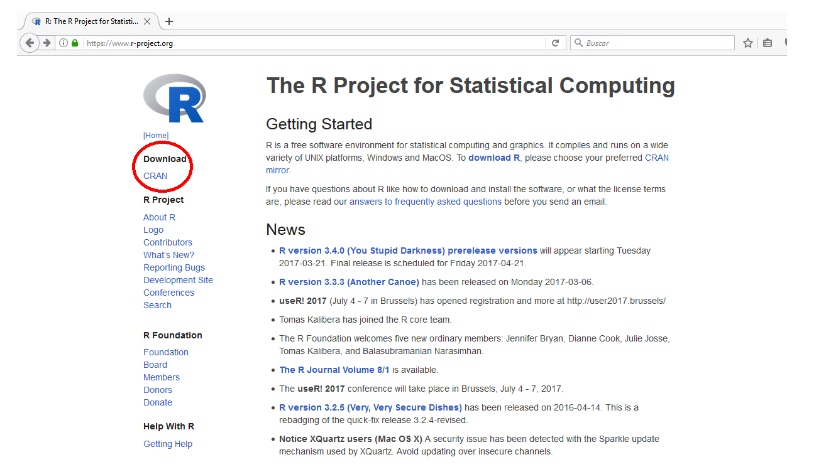
\includegraphics{imagenes/01.png}
\caption{Figura 1}
\end{figure}

Para descargar la aplicación hacemos clic en Cran y hacemos clic sobre el enlace del ``espejo'' más próximo a nuestra ubicación, México. Seleccionemos la URL de, por ejemplo (\url{https://cran.itam.mx/}).

\begin{figure}
\centering
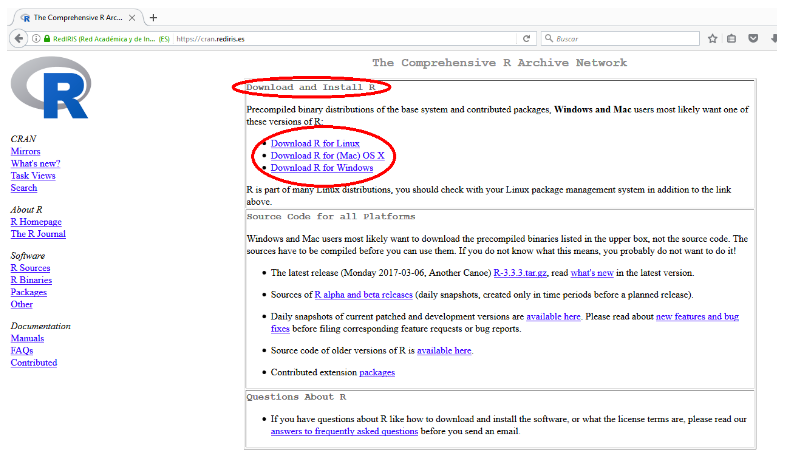
\includegraphics{imagenes/02.png}
\caption{Figura 2}
\end{figure}

Ahora, en función del tu sistema operativo, seleccionar la correspondiente opción.

\begin{figure}
\centering
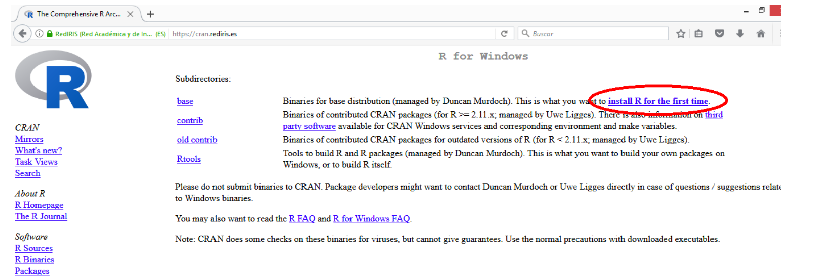
\includegraphics{imagenes/03.png}
\caption{Figura 3}
\end{figure}

\hypertarget{instalar-r-en-windows.}{%
\subsection{Instalar R en Windows.}\label{instalar-r-en-windows.}}

Al hacer clic sobre Download R for Windows iremos a la página que se reproduce más abajo. Hacer clic sobre \emph{install R for the first time.}

En la siguiente ventana, hacer clic sobre \emph{Download R 3.3.3 for Windows} y guardar el archivo de instalación.

Ejecutar el archivo descargado para proceder a la instalación de R.

\hypertarget{instalar-r-en-mac.}{%
\subsection{Instalar R en Mac.}\label{instalar-r-en-mac.}}

Al hacer clic sobre Download R for (Mac) OS X iremos a la página que se reproduce más abajo. Hacer clic sobre install R for the first time.

\begin{figure}
\centering
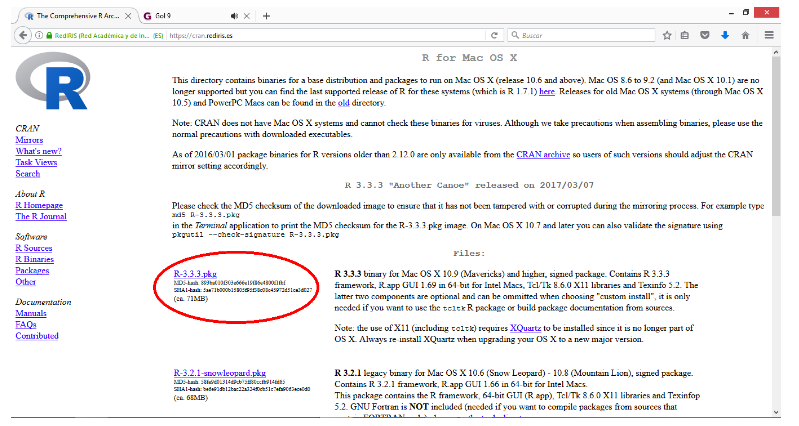
\includegraphics{imagenes/04.png}
\caption{Figura 4}
\end{figure}

Hacer clic sobre R-3.3.3.pkg y guardar el archivo de instalación. Ejecutar el archivo descargado para proceder a la instalación de R.

\hypertarget{instalar-rstudio}{%
\subsection{Instalar RStudio}\label{instalar-rstudio}}

Descargamos la aplicación desde la página web de RStudio \href{https://posit.co/download/rstudio-desktop/}{aquí} según nuestro sistema operativo de trabajo:

\begin{itemize}
\item
  RStudio 1.0.136 - Windows Vista/7/8/10.
\item
  RStudio 1.0.136 - Mac OS X 10.6+ (64-bit).
\end{itemize}

Una vez guardado el archivo, lo ejecutamos para instalar RStudio. Sigue las instrucciones de instalación.

\hypertarget{entorno-de-trabajo-de-rstudio.}{%
\section{Entorno de trabajo de RStudio.}\label{entorno-de-trabajo-de-rstudio.}}

En general trabajamos con la interfaz de RStudio antes que con la de R porque la primera es ``más amigable''.

Si abrimos RStudio vamos a ver algo parecido a lo que se muestra en la siguiente imagen:

\begin{figure}
\centering
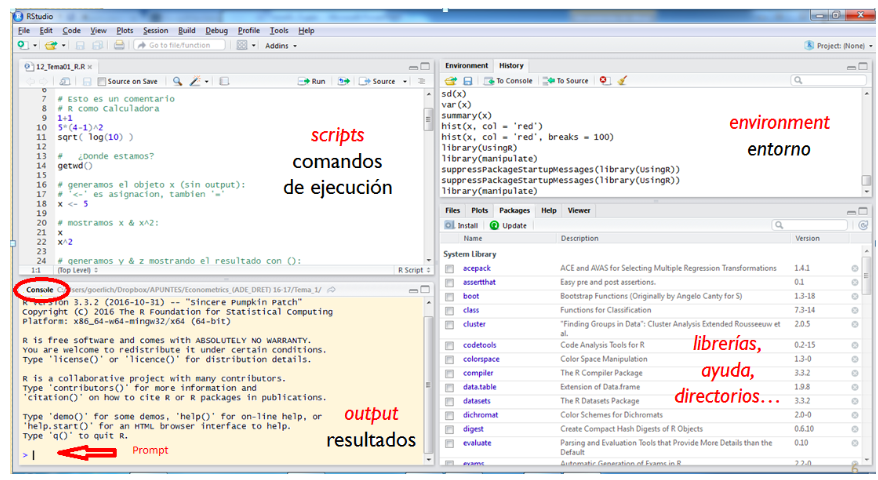
\includegraphics{imagenes/05.png}
\caption{Figura 5}
\end{figure}

Una vez estamos en RStudio, podemos escribir y ejecutar las órdenes de varias formas:

\begin{itemize}
\item
  directamente en la consola.
\item
  a través de un script (.R).
\item
  con archivos Rmarkdown (.Rmd).
\end{itemize}

Como podemos ver, RStudio está (normalmente) dividido en 4 paneles.

\hypertarget{consola}{%
\subsection{Consola}\label{consola}}

Por defecto, la consola se encuentra en el panel inferior-izquierdo. ¿Vemos la pestaña que pone Console? Inmediatamente debajo aparece un texto informativo y, finalmente, el símbolo ``\textgreater{}''. Aquí es donde R espera que le demos instrucciones. Para ejecutarlas y obtener el resultado pulsamos enter.

Vamos a hacer este ejemplo:

\begin{Shaded}
\begin{Highlighting}[]
\DecValTok{2}\SpecialCharTok{+}\DecValTok{2}
\end{Highlighting}
\end{Shaded}

\begin{verbatim}
## [1] 4
\end{verbatim}

\begin{Shaded}
\begin{Highlighting}[]
\DecValTok{5}\SpecialCharTok{*}\NormalTok{(}\DecValTok{3{-}1}\NormalTok{)}\SpecialCharTok{\^{}}\DecValTok{2}
\end{Highlighting}
\end{Shaded}

\begin{verbatim}
## [1] 20
\end{verbatim}

\begin{Shaded}
\begin{Highlighting}[]
\FunctionTok{sqrt}\NormalTok{(}\DecValTok{4}\NormalTok{)}
\end{Highlighting}
\end{Shaded}

\begin{verbatim}
## [1] 2
\end{verbatim}

\hypertarget{scripts}{%
\subsection{Scripts}\label{scripts}}

Trabajar en la consola es muy limitado ya que las instrucciones se han de introducir una a una. Lo habitual es trabajar con scripts o archivos de instrucciones. Estos archivos tienen extensión \textbf{.R}.

Se puede crear una script con cualquier editor de texto (uno de los más populares es Tinn-R), pero nosotros lo haremos desde RStudio. Para ello, seleccionamos la siguiente ruta de menús: \textbf{File \textgreater{} New File \textgreater{} R script}

\begin{figure}
\centering
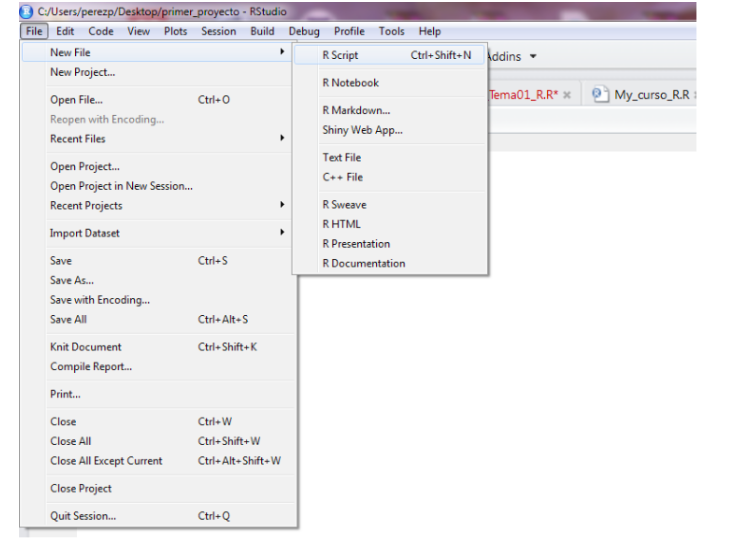
\includegraphics{imagenes/06.png}
\caption{Figura 5}
\end{figure}

El panel del script se sitúa en la parte superior-izquierda de RStudio. Ahora podemos escribir las instrucciones línea por línea. Las instrucciones las podemos ejecutar una a una o las podemos seleccionar y ejecutar en bloque. Para ejecutar las instrucciones tenemos varias alternativas:

\begin{itemize}
\item
  Hacemos clic en el botón: \textbf{Run} (botón situado en la parte derecha de las opciones del panel de script)
\item
  Pulsamos Ctrl+r
\item
  Ejecutamos el código desde las opciones del menú Code. Sinceramente, esto nunca lo hemos utilizado.
\end{itemize}

Como se muestra en la imagen más abajo, vamos a escribir nuestro primer script.

\begin{figure}
\centering
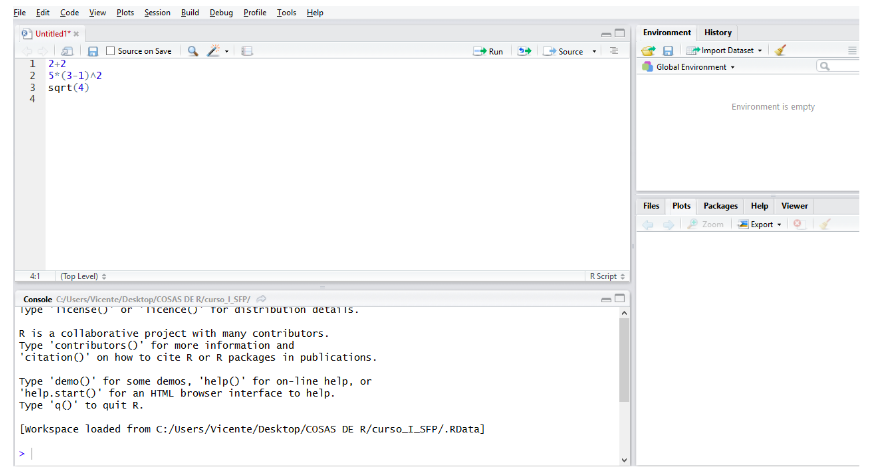
\includegraphics{imagenes/07.png}
\caption{Figura 6}
\end{figure}

Para guardar el script:

\begin{itemize}
\item
  File \textgreater{} Save as.. y seleccionar la ruta donde se quiere guardar el fichero.
\item
  Hacer clic en el botón Guardar que se encuentra en la parte izquierda de la cinta de opciones del script.
\end{itemize}

\hypertarget{entorno}{%
\subsection{Entorno}\label{entorno}}

El panel de entorno esta compuesto de dos pestañas: Environment y History.

\begin{itemize}
\tightlist
\item
  En el Environment se irán registrando los objetos que vayamos creando en la sesión de trabajo. También tenemos la opción de cargar y guardar una sesión de trabajo, importar datos y limpiar los objetos de la sesión. Estas opciones están accesibles a través de la cinta de opciones de la pestaña.
\end{itemize}

\begin{figure}
\centering
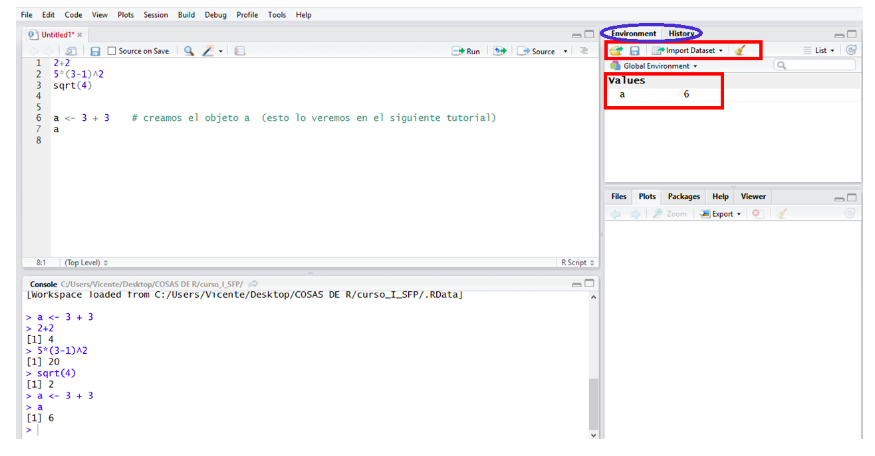
\includegraphics{imagenes/08.png}
\caption{Figura 7}
\end{figure}

\begin{itemize}
\tightlist
\item
  En la pestaña History se registran las instrucciones ejecutadas. Como opciones, podemos cargar y guardar el historial de la sesión, seleccionar una o más instrucciones y enviarlas bien a la consola bien al script, y limpiar el historial.
\end{itemize}

\hypertarget{otros-recursos}{%
\subsection{Otros recursos}\label{otros-recursos}}

Con el nombre de \textbf{Otros recursos} nos referimos al panel que se encuentra en la parte inferior-derecha del escritorio de RStudio.

En este panel cabe destacar las siguientes pestañas, cada una con diferentes opciones:

\begin{itemize}
\item
  Files: es una especie de explorador de archivos.
\item
  Plots: donde se visualizan los gráficos que creamos. Entre las opciones disponibles se encuentran:

  \begin{itemize}
  \tightlist
  \item
    Zoom: para agrandar el gráfico y verlo en otra ventana.
  \item
    Export: para exportar/guardar el gráfico. Se puede guardar el gráfico como imagen, pdf o copiarlo al portapapeles.
  \end{itemize}
\item
  Packages: proporciona un listado de los paquetes instalados en R y los que han sido cargado en la sesión. A través de las opciones de esta pestaña podemos instalar nuevos paquetes o actualizar los existentes.
\item
  Help: Para obtener ayuda sobre una determinada función.
\end{itemize}

\hypertarget{configuraciuxf3n-del-espacio-de-trabajo}{%
\section{Configuración del espacio de trabajo}\label{configuraciuxf3n-del-espacio-de-trabajo}}

Antes de comenzar a trabajar debemos fijar el directorio donde queremos guardar nuestros archivos. Básicamente, dos alternativas.

\hypertarget{opciuxf3n-1-fijar-directorio}{%
\subsection{Opción 1: Fijar directorio}\label{opciuxf3n-1-fijar-directorio}}

Opción 1. Indicamos a R la ruta donde queremos trabajar y la fijamos con la función setwd().

\begin{Shaded}
\begin{Highlighting}[]
\CommentTok{\#setwd("C:/ruta del directorio de trabajo")}
\end{Highlighting}
\end{Shaded}

Para comprobar el directorio de trabajo utilizamos la función getwd():

\begin{Shaded}
\begin{Highlighting}[]
\FunctionTok{getwd}\NormalTok{()}
\end{Highlighting}
\end{Shaded}

\begin{verbatim}
## [1] "/Users/user/Documents/proyectos/capacitacion/capacitacion_R"
\end{verbatim}

Para obtener un listado de los archivos que contiene la ruta establecida se usa la función dir().

\begin{Shaded}
\begin{Highlighting}[]
\FunctionTok{dir}\NormalTok{()}
\end{Highlighting}
\end{Shaded}

\begin{verbatim}
##  [1] "_book"               "_bookdown_files"     "_bookdown.yml"      
##  [4] "_main_files"         "_main.log"           "_main.Rmd"          
##  [7] "_output.yml"         "01_manipulacion.Rmd" "02_tarea.Rmd"       
## [10] "book.bib"            "capacitacion.Rproj"  "clase_2.R"          
## [13] "clase2.R"            "css"                 "data"               
## [16] "imagenes"            "index.Rmd"           "packages.bib"       
## [19] "preamble.tex"        "README.md"           "style.css"
\end{verbatim}

\hypertarget{opciuxf3n-2-proyecto-de-r.}{%
\section{Opción 2 : Proyecto de R.}\label{opciuxf3n-2-proyecto-de-r.}}

Al crear un proyecto todos los archivos quedan vinculados directamente al proyecto. Para crear un proyecto selección \textbf{File \textgreater{} New project\ldots{}} Se abrirá la siguiente ventana:

\begin{figure}
\centering
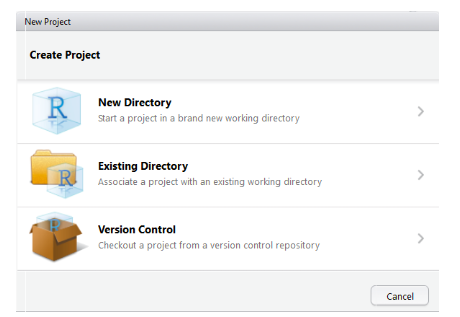
\includegraphics{imagenes/09.png}
\caption{Figura 8}
\end{figure}

Para crear un proyecto en un nuevo directorio, hacemos clic en el botón New Directory. En seguida, seleccionamos el tipo de proyecto, en nuestro caso Empty Project. Ahora, asignamos un nombre al directorio (carpeta) que se va a crear y que al mismo tiempo será el nombre del proyecto de R. Para terminar, hacemos clic en el botón Create Project. Al seguir este proceso se habrá creado una carpeta en Documentos y un fichero nombre\_carpeta.Rproj.

Para crear un proyecto en una carpeta que ya existe, hacemos clic en el botón Existing Directory y después seleccionamos la carpeta ayudándonos del Browse.. si fuera necesario. Una vez elegida la carpeta, clicamos en Create Project.

Para abrir un proyecto hacemos doble clic sobre el archivo con extensión .Rproj o lo abrimos desde el menú de RStudio: File \textgreater{} Open Project\ldots{}

Ventaja de los proyectos: cualquier fichero que creemos (script de R, documento de Rmarkdown, etc.) y guardemos se guardará en la carpeta del proyecto.

\hypertarget{instalaciuxf3n-de-paquetes.}{%
\section{Instalación de paquetes.}\label{instalaciuxf3n-de-paquetes.}}

R está compuesto por un sistema base, pero para extender su funcionalidad es necesario instalar paquetes adicionales.

Podemos instalar paquetes de varias formas:

\begin{itemize}
\item
  A través del menú: Tools \textgreater{} Install packages\ldots{}
\item
  En el escritorio de RStudio: Packages/Install. Vemos los paquetes que tenemos actualmente instalados y aquellos que se encuentran cargados.
\end{itemize}

\begin{figure}
\centering
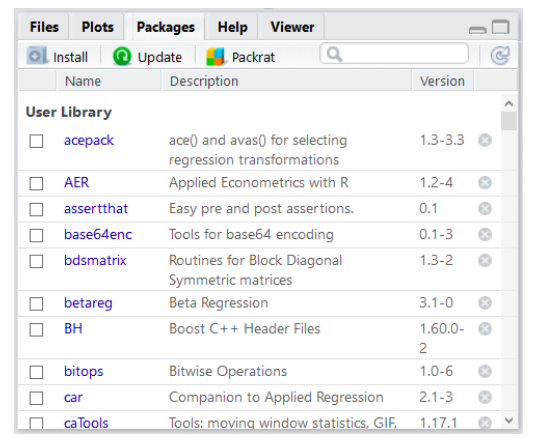
\includegraphics{imagenes/10.png}
\caption{Figura 9}
\end{figure}

\begin{itemize}
\tightlist
\item
  Utilizando la función install.packages(). El nombre del paquete que queremos instalar debe ir entre comillas.
\end{itemize}

\begin{Shaded}
\begin{Highlighting}[]
\CommentTok{\#install.packages("dplyr") \# dplyr es un paquete que se utiliza para manipular/gestionar datos}
\end{Highlighting}
\end{Shaded}

Una vez instalado el paquete, hay que cargarlo para poderlo utilizar. Esto se hace con la función library().

\begin{Shaded}
\begin{Highlighting}[]
\FunctionTok{library}\NormalTok{(dplyr)}
\end{Highlighting}
\end{Shaded}

\begin{verbatim}
## 
## Attaching package: 'dplyr'
\end{verbatim}

\begin{verbatim}
## The following objects are masked from 'package:stats':
## 
##     filter, lag
\end{verbatim}

\begin{verbatim}
## The following objects are masked from 'package:base':
## 
##     intersect, setdiff, setequal, union
\end{verbatim}

\hypertarget{ayuda-en-r.}{%
\section{Ayuda en R.}\label{ayuda-en-r.}}

En muchas ocasiones necesitamos ayuda sobre cómo funciona una determinada función, cuáles son sus argumentos, etc. Hay varias formas de pedir la ayuda de R. Vamos a pedir la ayuda de la función mean().

\begin{Shaded}
\begin{Highlighting}[]
\FunctionTok{help}\NormalTok{(mean)}
\NormalTok{?mean}
\end{Highlighting}
\end{Shaded}

Si ejecutamos directamente la función library() se abrirá una ventana listando los paquetes que tenemos instalados en R. En el escritorio de RStudio, en la pestaña Packages también tenemos en listado de paquetes instalados (organizados en dos bloques: User Library y System Library)

\begin{Shaded}
\begin{Highlighting}[]
\FunctionTok{library}\NormalTok{()}
\end{Highlighting}
\end{Shaded}

Para obtener ayuda sobre un determinado paquete\ldots{}

\begin{Shaded}
\begin{Highlighting}[]
\FunctionTok{library}\NormalTok{(}\AttributeTok{help=}\StringTok{"foreign"}\NormalTok{)}
\end{Highlighting}
\end{Shaded}

Pero sin duda, una de las mejores fuentes de ayuda en R nos la proporciona internet. Bien haciendo directamente en google la búsqueda sobre el tema que estamos interesados, bien acudiendo a algunas de las muchas webs que ofrecen ayuda. Algunas de las más populares y recomendables son:

\begin{itemize}
\item
  \href{https://www.r-bloggers.com/}{R-Bloggers}
\item
  \href{https://stackoverflow.com/}{Stack Overflow}
\end{itemize}

\hypertarget{comandos-buxe1sicos-de-r.}{%
\chapter{Comandos básicos de R.}\label{comandos-buxe1sicos-de-r.}}

\hypertarget{introducciuxf3n}{%
\section{Introducción}\label{introducciuxf3n}}

El objetivo de este tutorial es familiarizarnos con los conceptos básicos de R. ¿Qué es un objeto en R? ¿Con qué clases/tipos de objetos se trabaja en R?
Aprenderemos a definir vectores y operar con ellos; a crear matrices, listas y data frames; a seleccionar elementos, añadir filas y columnas, etc. Como lo que se pretende es que se entienda la filosofía y la práctica del trabajo con R, todos los conceptos que se introducen se ilustran con ejemplos muy sencillos. No obstante, la selección de funciones que se realiza en este tutorial tienen una aplicación directa en el tratamiento real de datos.

Vamos a realizar paso a paso este sencillo ejercicio para introducir algunos conceptos importantes.

\begin{Shaded}
\begin{Highlighting}[]
\DecValTok{3}\SpecialCharTok{+}\DecValTok{4}
\end{Highlighting}
\end{Shaded}

\begin{verbatim}
## [1] 7
\end{verbatim}

\begin{Shaded}
\begin{Highlighting}[]
\DocumentationTok{\#\# [1] 7}
\FunctionTok{log}\NormalTok{(}\DecValTok{10}\NormalTok{)}
\end{Highlighting}
\end{Shaded}

\begin{verbatim}
## [1] 2.302585
\end{verbatim}

\begin{Shaded}
\begin{Highlighting}[]
\DocumentationTok{\#\# [1] 2.302585}
\NormalTok{x }\OtherTok{\textless{}{-}} \DecValTok{3}\SpecialCharTok{+}\DecValTok{4}  
\NormalTok{x  }\CommentTok{\# x es un vector cuya primera componente es 7. Enseguida vamos con los vectores!}
\end{Highlighting}
\end{Shaded}

\begin{verbatim}
## [1] 7
\end{verbatim}

\begin{Shaded}
\begin{Highlighting}[]
\DocumentationTok{\#\# [1] 7}
\NormalTok{y }\OtherTok{=} \DecValTok{2}\SpecialCharTok{+}\DecValTok{6}
\NormalTok{y}
\end{Highlighting}
\end{Shaded}

\begin{verbatim}
## [1] 8
\end{verbatim}

\begin{Shaded}
\begin{Highlighting}[]
\DocumentationTok{\#\# [1] 8}
\NormalTok{z }\OtherTok{\textless{}{-}} \FunctionTok{c}\NormalTok{(x,y)}
\NormalTok{z}
\end{Highlighting}
\end{Shaded}

\begin{verbatim}
## [1] 7 8
\end{verbatim}

\begin{Shaded}
\begin{Highlighting}[]
\DocumentationTok{\#\# [1] 7 8}
\FunctionTok{mean}\NormalTok{(z)}
\end{Highlighting}
\end{Shaded}

\begin{verbatim}
## [1] 7.5
\end{verbatim}

\begin{Shaded}
\begin{Highlighting}[]
\DocumentationTok{\#\# [1] 7.5}
\NormalTok{w }\OtherTok{\textless{}{-}} \FunctionTok{mean}\NormalTok{(z)}
\NormalTok{w}
\end{Highlighting}
\end{Shaded}

\begin{verbatim}
## [1] 7.5
\end{verbatim}

\begin{Shaded}
\begin{Highlighting}[]
\DocumentationTok{\#\# [1] 7.5}
\FunctionTok{round}\NormalTok{(w, }\AttributeTok{digits=}\DecValTok{0}\NormalTok{)}
\end{Highlighting}
\end{Shaded}

\begin{verbatim}
## [1] 8
\end{verbatim}

\begin{Shaded}
\begin{Highlighting}[]
\DocumentationTok{\#\# [1] 8}
\end{Highlighting}
\end{Shaded}

R utiliza funciones para realizar operaciones. Una función es, por ejemplo, mean(). Para utilizar una función deben especificarse unos argumentos, que es lo que escribimos dentro de los paréntesis. En el caso de la función round() hemos especificado dos argumentos: el vector que queremos redondear (w) y el número de decimales del redondeo (digits).

\textbf{El símbolo \textless- es el operador para asignar. También se puede utilizar = (o menos frecuente -\textgreater), aunque es preferible utilizar el \textless-.}

El símbolo \textbf{\#} se utiliza para introducir un comentario. \textbf{Todo lo que quede a la derecha de \# no se ejecutará.}

Cuando se realiza una asignación se obtiene un objeto. Podemos ver el resultado o contenido de un objeto de varias formas. Por ejemplo, para ver qué es el objeto x podemos escribir en la consola:

\begin{itemize}
\item
  x
\item
  print(x)
\item
  (x \textless- 3+4)
\end{itemize}

\hypertarget{vectores}{%
\section{Vectores}\label{vectores}}

Básicamente R trabaja con los siguientes tipos de objetos:

\begin{itemize}
\item
  VECTORES
\item
  MATRICES y ARRAYS (variables indexadas)
\item
  LISTAS
\item
  FACTORES
\item
  DATA FRAMES
\item
  FUNCIONES
\end{itemize}

Empezaremos viendo los objetos más sencillos, los vectores. Poco a poco iremos viendo el resto de objetos.

La mayoría de las operaciones (+, -, *, /) y funciones en R están definidas con carácter vectorial. ¿Qué significa esto? Que R opera componente a componente.

Antes de entender el concepto ``caracter vectorial'', vamos a ver cómo se define/crea un vector.

Para crear un vector se utiliza la función c() (c de concatenate). Por ejemplo:

\begin{Shaded}
\begin{Highlighting}[]
\NormalTok{x }\OtherTok{\textless{}{-}} \FunctionTok{c}\NormalTok{(}\DecValTok{1}\NormalTok{,}\DecValTok{2}\NormalTok{,}\DecValTok{3}\NormalTok{,}\DecValTok{4}\NormalTok{)}
\NormalTok{x                  }\CommentTok{\# x es un vector que tiene cuatro componentes}
\end{Highlighting}
\end{Shaded}

\begin{verbatim}
## [1] 1 2 3 4
\end{verbatim}

\begin{Shaded}
\begin{Highlighting}[]
\NormalTok{y }\OtherTok{\textless{}{-}} \FunctionTok{c}\NormalTok{(}\DecValTok{5}\NormalTok{,}\DecValTok{6}\NormalTok{,}\DecValTok{7}\NormalTok{,}\DecValTok{8}\NormalTok{)}
\NormalTok{y}
\end{Highlighting}
\end{Shaded}

\begin{verbatim}
## [1] 5 6 7 8
\end{verbatim}

Volvemos sobre el tema del carácter vectorial, es decir, se opera componente a componente. Pensemos, si

\begin{Shaded}
\begin{Highlighting}[]
\NormalTok{z }\OtherTok{\textless{}{-}}\NormalTok{ x }\SpecialCharTok{+}\NormalTok{ y}
\end{Highlighting}
\end{Shaded}

¿Qué resultado espero obtener para z?

Exacto!!! Como la operación se realiza vectorialmente (componente a componente, muy importante!) el resultado es:

\begin{Shaded}
\begin{Highlighting}[]
\NormalTok{z}
\end{Highlighting}
\end{Shaded}

\begin{verbatim}
## [1]  6  8 10 12
\end{verbatim}

Vamos a ver si lo entendemos de verdad. Supongamos que x e y son los siguientes vectores:

\begin{Shaded}
\begin{Highlighting}[]
\NormalTok{x }\OtherTok{\textless{}{-}} \FunctionTok{c}\NormalTok{(}\DecValTok{1}\NormalTok{,}\DecValTok{2}\NormalTok{,}\DecValTok{3}\NormalTok{,}\DecValTok{4}\NormalTok{)}
\NormalTok{y }\OtherTok{\textless{}{-}} \FunctionTok{c}\NormalTok{(}\DecValTok{1}\NormalTok{,}\DecValTok{2}\NormalTok{,}\DecValTok{3}\NormalTok{)}
\end{Highlighting}
\end{Shaded}

¿Qué longitud tienen los vectores x e y? Aquí la respuesta está clara, pero en aplicaciones reales utilizaríamos la función length().

\begin{Shaded}
\begin{Highlighting}[]
\FunctionTok{length}\NormalTok{(x)                }\CommentTok{\# esta función es muy útil, conviene recordarla.}
\end{Highlighting}
\end{Shaded}

\begin{verbatim}
## [1] 4
\end{verbatim}

\begin{Shaded}
\begin{Highlighting}[]
\DocumentationTok{\#\# [1] 4}
\FunctionTok{length}\NormalTok{(y)}
\end{Highlighting}
\end{Shaded}

\begin{verbatim}
## [1] 3
\end{verbatim}

\begin{Shaded}
\begin{Highlighting}[]
\DocumentationTok{\#\# [1] 3}
\end{Highlighting}
\end{Shaded}

Los vectores no tienen la misma longitud, entonces.. ¿Cuál será el resultado de z \textless- x + y?

\begin{Shaded}
\begin{Highlighting}[]
\NormalTok{z }\OtherTok{\textless{}{-}}\NormalTok{ x}\SpecialCharTok{+}\NormalTok{y}
\end{Highlighting}
\end{Shaded}

\begin{verbatim}
## Warning in x + y: longer object length is not a multiple of shorter object
## length
\end{verbatim}

\begin{Shaded}
\begin{Highlighting}[]
\NormalTok{z}
\end{Highlighting}
\end{Shaded}

\begin{verbatim}
## [1] 2 4 6 5
\end{verbatim}

R nos da un mensaje de aviso (warning), no es lo mismo que un error. Nos avisa que hay algo que no cuadra pero\ldots realiza la operación que nosotros queremos.

Una cuestión muy importante que siempre tenemos que tener en cuenta cuando trabajamos con vectores es que en un vector sólo podemos concatenar elementos del mismo tipo. ¿Qué tipos/clases de elementos (o datos) tenemos en R?

\begin{itemize}
\item
  Carácter
\item
  Numéricos
\item
  Enteros
\item
  Complejos
\item
  Lógicos
\end{itemize}

Veamos algunos ejemplos\ldots{}

\begin{Shaded}
\begin{Highlighting}[]
\NormalTok{x }\OtherTok{\textless{}{-}} \FunctionTok{c}\NormalTok{(}\DecValTok{1}\NormalTok{,}\DecValTok{2}\NormalTok{,}\DecValTok{3}\NormalTok{,}\DecValTok{4}\NormalTok{)    }\CommentTok{\# creamos el vector x}
\FunctionTok{class}\NormalTok{(x)           }\CommentTok{\# devuelve el tipo de objeto}
\end{Highlighting}
\end{Shaded}

\begin{verbatim}
## [1] "numeric"
\end{verbatim}

\begin{Shaded}
\begin{Highlighting}[]
\NormalTok{y }\OtherTok{\textless{}{-}} \FunctionTok{c}\NormalTok{(}\StringTok{"a"}\NormalTok{,}\StringTok{"b"}\NormalTok{)}
\FunctionTok{class}\NormalTok{(y)}
\end{Highlighting}
\end{Shaded}

\begin{verbatim}
## [1] "character"
\end{verbatim}

\begin{Shaded}
\begin{Highlighting}[]
\NormalTok{z }\OtherTok{\textless{}{-}} \FunctionTok{c}\NormalTok{(1L,2L,3L)   }\CommentTok{\# escribimos L detrás del número para obligar a que sea entero}
\FunctionTok{class}\NormalTok{(z)}
\end{Highlighting}
\end{Shaded}

\begin{verbatim}
## [1] "integer"
\end{verbatim}

\begin{Shaded}
\begin{Highlighting}[]
\NormalTok{w }\OtherTok{\textless{}{-}} \FunctionTok{c}\NormalTok{(}\ConstantTok{TRUE}\NormalTok{, F)    }\CommentTok{\# en general, puede escribirse TRUE/FALSE o T/F}
\FunctionTok{class}\NormalTok{(w)}
\end{Highlighting}
\end{Shaded}

\begin{verbatim}
## [1] "logical"
\end{verbatim}

\begin{Shaded}
\begin{Highlighting}[]
\NormalTok{t }\OtherTok{\textless{}{-}} \FunctionTok{c}\NormalTok{(}\DecValTok{1}\SpecialCharTok{+}\NormalTok{2i, }\DecValTok{1}\SpecialCharTok{+}\NormalTok{3i)}
\FunctionTok{class}\NormalTok{(t)}
\end{Highlighting}
\end{Shaded}

\begin{verbatim}
## [1] "complex"
\end{verbatim}

En los ejemplos anteriores hemos definido un vector en el que todos sus elementos eran del mismo tipo. Pero\ldots.¿qué pasa si tenemos los siguientes vectores?

\begin{Shaded}
\begin{Highlighting}[]
\NormalTok{x }\OtherTok{\textless{}{-}} \FunctionTok{c}\NormalTok{(}\DecValTok{1}\NormalTok{,}\DecValTok{2}\NormalTok{,}\StringTok{"a"}\NormalTok{)}
\NormalTok{y }\OtherTok{\textless{}{-}} \FunctionTok{c}\NormalTok{(}\ConstantTok{FALSE}\NormalTok{, }\DecValTok{1}\NormalTok{)}
\NormalTok{z }\OtherTok{\textless{}{-}} \FunctionTok{c}\NormalTok{(}\StringTok{"a"}\NormalTok{,T)}
\end{Highlighting}
\end{Shaded}

¿De qué tipo son ahora los vectores x, y, z?

\begin{Shaded}
\begin{Highlighting}[]
\FunctionTok{class}\NormalTok{(x)}
\end{Highlighting}
\end{Shaded}

\begin{verbatim}
## [1] "character"
\end{verbatim}

\begin{Shaded}
\begin{Highlighting}[]
\DocumentationTok{\#\# [1] "character"}
\FunctionTok{class}\NormalTok{(y)}
\end{Highlighting}
\end{Shaded}

\begin{verbatim}
## [1] "numeric"
\end{verbatim}

\begin{Shaded}
\begin{Highlighting}[]
\DocumentationTok{\#\# [1] "numeric"}
\FunctionTok{class}\NormalTok{(z)}
\end{Highlighting}
\end{Shaded}

\begin{verbatim}
## [1] "character"
\end{verbatim}

\begin{Shaded}
\begin{Highlighting}[]
\DocumentationTok{\#\# [1] "character"}
\end{Highlighting}
\end{Shaded}

R ha forzado a que todos los elementos del vector sean del mismo tipo. A esto se le llama implicit coercion. Fijémonos cúal es el resultado de los vectores que hemos definido antes.

\begin{Shaded}
\begin{Highlighting}[]
\NormalTok{x}
\end{Highlighting}
\end{Shaded}

\begin{verbatim}
## [1] "1" "2" "a"
\end{verbatim}

\begin{Shaded}
\begin{Highlighting}[]
\NormalTok{y}
\end{Highlighting}
\end{Shaded}

\begin{verbatim}
## [1] 0 1
\end{verbatim}

\begin{Shaded}
\begin{Highlighting}[]
\NormalTok{z}
\end{Highlighting}
\end{Shaded}

\begin{verbatim}
## [1] "a"    "TRUE"
\end{verbatim}

En ocasiones somos nosotros los que estamos interesados en forzar que todos los elementos del vector sean del mismo tipo (esto es la explicit coercion). Para ello utilizamos las funciones as.numeric() , as.character(), as.logical() \ldots{} Si el resultado no tiene sentido R producirá un mensaje de error o warning. Un ejemplo:

\begin{Shaded}
\begin{Highlighting}[]
\NormalTok{x }\OtherTok{\textless{}{-}} \FunctionTok{c}\NormalTok{(}\DecValTok{1}\NormalTok{,}\DecValTok{2}\NormalTok{,}\StringTok{"a"}\NormalTok{)}
\NormalTok{x}
\end{Highlighting}
\end{Shaded}

\begin{verbatim}
## [1] "1" "2" "a"
\end{verbatim}

\begin{Shaded}
\begin{Highlighting}[]
\DocumentationTok{\#\# [1] "1" "2" "a"}
\FunctionTok{as.numeric}\NormalTok{(x)}
\end{Highlighting}
\end{Shaded}

\begin{verbatim}
## Warning: NAs introduced by coercion
\end{verbatim}

\begin{verbatim}
## [1]  1  2 NA
\end{verbatim}

\begin{Shaded}
\begin{Highlighting}[]
\DocumentationTok{\#\# [1]  1  2 NA}
\FunctionTok{as.character}\NormalTok{(x)}
\end{Highlighting}
\end{Shaded}

\begin{verbatim}
## [1] "1" "2" "a"
\end{verbatim}

\begin{Shaded}
\begin{Highlighting}[]
\DocumentationTok{\#\# [1] "1" "2" "a"}
\end{Highlighting}
\end{Shaded}

Por último, podemos evaluar el tipo/clase de objeto con las funciones is.numeric(), is.character(), etc.

\hypertarget{acceder-a-un-elemento-de-un-objeto}{%
\subsection{Acceder a un elemento de un objeto}\label{acceder-a-un-elemento-de-un-objeto}}

Para seleccionar/acceder a un elemento de un objeto se suelen emplear: \textbf{{[}{]}, \$, {[}{[}{]}{]}.}

Vamos a crear el objeto x que será un vector de cuatro componentes formado por los cuatro primeros números pares. Así:

\begin{Shaded}
\begin{Highlighting}[]
\NormalTok{x }\OtherTok{\textless{}{-}} \FunctionTok{c}\NormalTok{(}\DecValTok{2}\NormalTok{,}\DecValTok{4}\NormalTok{,}\DecValTok{6}\NormalTok{,}\DecValTok{8}\NormalTok{)}
\end{Highlighting}
\end{Shaded}

Si queremos acceder/seleccionar/extraer al/el segundo componente de x

\begin{Shaded}
\begin{Highlighting}[]
\NormalTok{x[}\DecValTok{2}\NormalTok{]}
\end{Highlighting}
\end{Shaded}

\begin{verbatim}
## [1] 4
\end{verbatim}

\hypertarget{enlistar-y-borrar-objetos}{%
\subsection{Enlistar y borrar objetos}\label{enlistar-y-borrar-objetos}}

Las funciones ls() y objects() hacen lo mismo: listan los objetos que hemos definido en la sesión.

\begin{Shaded}
\begin{Highlighting}[]
\FunctionTok{ls}\NormalTok{()}
\end{Highlighting}
\end{Shaded}

\begin{verbatim}
## [1] "t" "w" "x" "y" "z"
\end{verbatim}

\begin{Shaded}
\begin{Highlighting}[]
\FunctionTok{objects}\NormalTok{()}
\end{Highlighting}
\end{Shaded}

\begin{verbatim}
## [1] "t" "w" "x" "y" "z"
\end{verbatim}

Si queremos borrar objetos utilizamos la función rm()

\begin{Shaded}
\begin{Highlighting}[]
\FunctionTok{rm}\NormalTok{(z)  }\CommentTok{\# borramos el objeto z}
\FunctionTok{ls}\NormalTok{()}
\end{Highlighting}
\end{Shaded}

\begin{verbatim}
## [1] "t" "w" "x" "y"
\end{verbatim}

y si estamos interesados en borrar todos los objetos que hemos definido:

\begin{Shaded}
\begin{Highlighting}[]
\FunctionTok{rm}\NormalTok{(}\AttributeTok{list=}\FunctionTok{ls}\NormalTok{()) }\CommentTok{\# o también rm(list=objects())}
\FunctionTok{ls}\NormalTok{()}
\end{Highlighting}
\end{Shaded}

\begin{verbatim}
## character(0)
\end{verbatim}

\hypertarget{ejercicios}{%
\subsubsection{Ejercicios}\label{ejercicios}}

\begin{itemize}
\tightlist
\item
  Crea un vector x con 5 elementos numéricos.
\item
  Crea un vector y con 5 elementos de tipo caractér.
\item
  ¿De qué tipo es el siguiente vector?:
\end{itemize}

\begin{Shaded}
\begin{Highlighting}[]
\NormalTok{z }\OtherTok{\textless{}{-}} \FunctionTok{c}\NormalTok{(}\StringTok{"32"}\NormalTok{,}\StringTok{"52"}\NormalTok{,}\StringTok{"6"}\NormalTok{,}\StringTok{"82"}\NormalTok{,}\StringTok{"12"}\NormalTok{)}
\end{Highlighting}
\end{Shaded}

\begin{itemize}
\tightlist
\item
  Suma el vector x y el vector z ¿Tienes que hacer alguna transformación?
\item
  Multiplica el vector z por 3 y después súmalo al vector x.
\end{itemize}

\hypertarget{tipos-de-objetos}{%
\section{Tipos de objetos}\label{tipos-de-objetos}}

\hypertarget{matrices}{%
\subsection{Matrices}\label{matrices}}

La función matrix() permite organizar los datos en una matriz con tantas filas y columnas como se indiquen.

Vamos a pedir ayuda a R sobre la función matrix()

\begin{Shaded}
\begin{Highlighting}[]
\NormalTok{?matrix }\CommentTok{\# una forma de obtener ayuda en R es escribiendo ? delante de la función de la que solicitamos ayuda}
\end{Highlighting}
\end{Shaded}

\hypertarget{cuxf3mo-crear-y-trabajar-con-matrices}{%
\subsubsection{Cómo crear y trabajar con matrices}\label{cuxf3mo-crear-y-trabajar-con-matrices}}

Una vez hemos leído en la ayuda cómo usar la función matrix, vamos a practicarlo con el siguiente ejemplo. Pero antes de ejecutarlo, pensemos en qué es lo que queremos hacer y, sobre todo, pensemos en cuál es el resultado que esperamos obtener.

\begin{Shaded}
\begin{Highlighting}[]
\NormalTok{x }\OtherTok{\textless{}{-}} \FunctionTok{matrix}\NormalTok{ (}\AttributeTok{data=} \FunctionTok{c}\NormalTok{(}\DecValTok{1}\NormalTok{,}\DecValTok{2}\NormalTok{,}\DecValTok{3}\NormalTok{,}\DecValTok{4}\NormalTok{), }\AttributeTok{nrow=}\DecValTok{2}\NormalTok{, }\AttributeTok{ncol=}\DecValTok{2}\NormalTok{) }\CommentTok{\# o x \textless{}{-} matrix (c(1,2,3,4), nrow=2, ncol=2)}
\NormalTok{x}
\end{Highlighting}
\end{Shaded}

\begin{verbatim}
##      [,1] [,2]
## [1,]    1    3
## [2,]    2    4
\end{verbatim}

Observemos que se ha creado una matrix de 2x2 (2 filas y 2 columnas) y, además, muy importante, ¿cómo se ha completado la matriz? ¡Exacto! La matriz se ha rellenado por columnas. Si queremos que se rellene por filas hay que incluir el argumento byrow en los argumentos de la función.

\begin{Shaded}
\begin{Highlighting}[]
\NormalTok{y }\OtherTok{\textless{}{-}} \FunctionTok{matrix}\NormalTok{ (}\FunctionTok{c}\NormalTok{(}\DecValTok{1}\NormalTok{,}\DecValTok{2}\NormalTok{,}\DecValTok{3}\NormalTok{,}\DecValTok{4}\NormalTok{), }\AttributeTok{nrow=}\DecValTok{2}\NormalTok{, }\AttributeTok{ncol=}\DecValTok{2}\NormalTok{, }\AttributeTok{byrow=}\NormalTok{T)}
\NormalTok{y}
\end{Highlighting}
\end{Shaded}

\begin{verbatim}
##      [,1] [,2]
## [1,]    1    2
## [2,]    3    4
\end{verbatim}

Fíjense en la diferencia entre los objetos x e y.

Una forma más simple para definir una matrix es:

\begin{Shaded}
\begin{Highlighting}[]
\NormalTok{y }\OtherTok{\textless{}{-}} \FunctionTok{matrix}\NormalTok{ (}\FunctionTok{c}\NormalTok{(}\DecValTok{1}\NormalTok{,}\DecValTok{2}\NormalTok{,}\DecValTok{3}\NormalTok{,}\DecValTok{4}\NormalTok{), }\DecValTok{2}\NormalTok{, }\DecValTok{2}\NormalTok{, }\AttributeTok{byrow=}\NormalTok{T)}
\NormalTok{y}
\end{Highlighting}
\end{Shaded}

\begin{verbatim}
##      [,1] [,2]
## [1,]    1    2
## [2,]    3    4
\end{verbatim}

aunque también podíamos haber omitido el argumento relativo al número de filas o de columnas, porque conocida una dimensión R completaría la matrix dados los datos con los que se trabaja.

\begin{Shaded}
\begin{Highlighting}[]
\NormalTok{y }\OtherTok{\textless{}{-}} \FunctionTok{matrix}\NormalTok{ (}\FunctionTok{c}\NormalTok{(}\DecValTok{1}\NormalTok{,}\DecValTok{2}\NormalTok{,}\DecValTok{3}\NormalTok{,}\DecValTok{4}\NormalTok{), }\DecValTok{2}\NormalTok{, }\AttributeTok{byrow=}\NormalTok{T)  }\CommentTok{\# no especificamos nrow porque por defecto es el primer argumento después de los datos}
\NormalTok{y}
\end{Highlighting}
\end{Shaded}

\begin{verbatim}
##      [,1] [,2]
## [1,]    1    2
## [2,]    3    4
\end{verbatim}

\begin{Shaded}
\begin{Highlighting}[]
\NormalTok{x }\OtherTok{\textless{}{-}} \FunctionTok{matrix}\NormalTok{(}\FunctionTok{c}\NormalTok{(}\DecValTok{1}\NormalTok{,}\DecValTok{2}\NormalTok{,}\DecValTok{3}\NormalTok{,}\DecValTok{4}\NormalTok{,}\DecValTok{5}\NormalTok{,}\DecValTok{6}\NormalTok{), }\AttributeTok{ncol=}\DecValTok{3}\NormalTok{)}
\NormalTok{x}
\end{Highlighting}
\end{Shaded}

\begin{verbatim}
##      [,1] [,2] [,3]
## [1,]    1    3    5
## [2,]    2    4    6
\end{verbatim}

\hypertarget{seleccionando-elementos-de-una-matriz}{%
\subsubsection{Seleccionando elementos de una matriz}\label{seleccionando-elementos-de-una-matriz}}

Lo primero, vamos a crear el objeto A que será una matriz.

\begin{Shaded}
\begin{Highlighting}[]
\NormalTok{A }\OtherTok{\textless{}{-}} \FunctionTok{matrix}\NormalTok{(}\DecValTok{1}\SpecialCharTok{:}\DecValTok{16}\NormalTok{,}\DecValTok{4}\NormalTok{,}\DecValTok{4}\NormalTok{)}
\NormalTok{A}
\end{Highlighting}
\end{Shaded}

\begin{verbatim}
##      [,1] [,2] [,3] [,4]
## [1,]    1    5    9   13
## [2,]    2    6   10   14
## [3,]    3    7   11   15
## [4,]    4    8   12   16
\end{verbatim}

Para seleccionar elementos de una matriz utilizamos el símbolo de los corchetes: {[}{]}.

Pensemos un momento en el posible resultado de estos ejemplos antes de efectuarlos.

\begin{Shaded}
\begin{Highlighting}[]
\NormalTok{A[}\DecValTok{2}\NormalTok{,}\DecValTok{3}\NormalTok{]}
\end{Highlighting}
\end{Shaded}

\begin{verbatim}
## [1] 10
\end{verbatim}

\begin{Shaded}
\begin{Highlighting}[]
\NormalTok{A[}\FunctionTok{c}\NormalTok{(}\DecValTok{1}\NormalTok{,}\DecValTok{2}\NormalTok{),}\FunctionTok{c}\NormalTok{(}\DecValTok{2}\NormalTok{,}\DecValTok{4}\NormalTok{)]}
\end{Highlighting}
\end{Shaded}

\begin{verbatim}
##      [,1] [,2]
## [1,]    5   13
## [2,]    6   14
\end{verbatim}

\begin{Shaded}
\begin{Highlighting}[]
\NormalTok{A[}\DecValTok{1}\SpecialCharTok{:}\DecValTok{3}\NormalTok{,}\DecValTok{2}\SpecialCharTok{:}\DecValTok{4}\NormalTok{]}
\end{Highlighting}
\end{Shaded}

\begin{verbatim}
##      [,1] [,2] [,3]
## [1,]    5    9   13
## [2,]    6   10   14
## [3,]    7   11   15
\end{verbatim}

\begin{Shaded}
\begin{Highlighting}[]
\NormalTok{A[}\DecValTok{1}\NormalTok{,]}
\end{Highlighting}
\end{Shaded}

\begin{verbatim}
## [1]  1  5  9 13
\end{verbatim}

\begin{Shaded}
\begin{Highlighting}[]
\NormalTok{A[}\DecValTok{1}\SpecialCharTok{:}\DecValTok{2}\NormalTok{,]}
\end{Highlighting}
\end{Shaded}

\begin{verbatim}
##      [,1] [,2] [,3] [,4]
## [1,]    1    5    9   13
## [2,]    2    6   10   14
\end{verbatim}

\begin{Shaded}
\begin{Highlighting}[]
\NormalTok{A[,}\DecValTok{2}\SpecialCharTok{:}\DecValTok{3}\NormalTok{]}
\end{Highlighting}
\end{Shaded}

\begin{verbatim}
##      [,1] [,2]
## [1,]    5    9
## [2,]    6   10
## [3,]    7   11
## [4,]    8   12
\end{verbatim}

\hypertarget{listas}{%
\subsection{Listas}\label{listas}}

A diferencia de los vectores o matrices, las listas pueden contener elementos/componentes de distinto tipo. Observemos esta lista que tiene 5 componentes (pueden ser matrices, vectores, dataframes,..).

\begin{Shaded}
\begin{Highlighting}[]
\NormalTok{x }\OtherTok{\textless{}{-}} \FunctionTok{list}\NormalTok{(}\FunctionTok{c}\NormalTok{(}\DecValTok{1}\NormalTok{,}\DecValTok{2}\NormalTok{,}\DecValTok{3}\NormalTok{,}\DecValTok{4}\NormalTok{), }\StringTok{"Curso"}\NormalTok{, F, }\DecValTok{1}\SpecialCharTok{+}\NormalTok{2i, 3L,A)}
\NormalTok{x}
\end{Highlighting}
\end{Shaded}

\begin{verbatim}
## [[1]]
## [1] 1 2 3 4
## 
## [[2]]
## [1] "Curso"
## 
## [[3]]
## [1] FALSE
## 
## [[4]]
## [1] 1+2i
## 
## [[5]]
## [1] 3
## 
## [[6]]
##      [,1] [,2] [,3] [,4]
## [1,]    1    5    9   13
## [2,]    2    6   10   14
## [3,]    3    7   11   15
## [4,]    4    8   12   16
\end{verbatim}

Utilizamos el doble corchete {[}{[}{]}{]} para acceder al contenido concreto de una lista.

\begin{Shaded}
\begin{Highlighting}[]
\NormalTok{x[[}\DecValTok{3}\NormalTok{]]  }\CommentTok{\# accedemos al tercer componente de la lista}
\end{Highlighting}
\end{Shaded}

\begin{verbatim}
## [1] FALSE
\end{verbatim}

\begin{Shaded}
\begin{Highlighting}[]
\NormalTok{x[[}\DecValTok{1}\NormalTok{]][}\DecValTok{2}\NormalTok{] }\CommentTok{\# accedemos al segundo elemento del primer componente de la lista}
\end{Highlighting}
\end{Shaded}

\begin{verbatim}
## [1] 2
\end{verbatim}

\begin{Shaded}
\begin{Highlighting}[]
\NormalTok{x[[}\DecValTok{6}\NormalTok{]][}\DecValTok{1}\NormalTok{,}\DecValTok{2}\NormalTok{]}
\end{Highlighting}
\end{Shaded}

\begin{verbatim}
## [1] 5
\end{verbatim}

Vamos a crear otra lista para practicar.

\begin{Shaded}
\begin{Highlighting}[]
\NormalTok{y }\OtherTok{\textless{}{-}} \FunctionTok{list}\NormalTok{( }\AttributeTok{Titulacion =} \FunctionTok{c}\NormalTok{(}\StringTok{"Economía"}\NormalTok{, }\StringTok{"Sociología"}\NormalTok{, }\StringTok{"Derecho"}\NormalTok{), }\AttributeTok{Edad =}\FunctionTok{c}\NormalTok{(}\DecValTok{25}\NormalTok{,}\DecValTok{26}\NormalTok{,}\DecValTok{27}\NormalTok{))}

\NormalTok{y}
\end{Highlighting}
\end{Shaded}

\begin{verbatim}
## $Titulacion
## [1] "Economía"   "Sociología" "Derecho"   
## 
## $Edad
## [1] 25 26 27
\end{verbatim}

Fijémonos en la diferencia de presentación de las listas x e y. Como en la lista y hemos nombrado los componentes, estos aparecen al ejecutar el objeto precedidos del símbolo \$. Ahora también podemos acceder a un componente de la lista por su nombre.

\begin{Shaded}
\begin{Highlighting}[]
\NormalTok{y}\SpecialCharTok{$}\NormalTok{Titulacion}
\end{Highlighting}
\end{Shaded}

\begin{verbatim}
## [1] "Economía"   "Sociología" "Derecho"
\end{verbatim}

\begin{Shaded}
\begin{Highlighting}[]
\NormalTok{y[[}\DecValTok{1}\NormalTok{]]}
\end{Highlighting}
\end{Shaded}

\begin{verbatim}
## [1] "Economía"   "Sociología" "Derecho"
\end{verbatim}

Evidentemente, también podemos realizar operaciones con listas.

\begin{Shaded}
\begin{Highlighting}[]
\NormalTok{y[[}\DecValTok{2}\NormalTok{]]}\SpecialCharTok{*}\DecValTok{3}
\end{Highlighting}
\end{Shaded}

\begin{verbatim}
## [1] 75 78 81
\end{verbatim}

\hypertarget{ejercicios-1}{%
\subsubsection{Ejercicios}\label{ejercicios-1}}

\begin{itemize}
\tightlist
\item
  Crea dos matrices A y B de dimensión 3x3.
\item
  Suma las dos matrices ¿Qué obtuviste?
\item
  Multiplica las las dos matrices ¿Qué obtuviste?
\item
  Trata de definir una matriz con valores tipo caractér.
\item
  Crea una lista con los siguientes elementos: un número, un vector, una matrix y una palabra.
\item
  Obten el elemento de la lista que es una matriz y multiplícalo por la matriz B.
\end{itemize}

\hypertarget{data-frame}{%
\subsection{Data Frame}\label{data-frame}}

Los data frame se usan para almacenar datos en forma de tablas (filas / columnas), como estamos habituados en Excel, Spss, etc.

Los data frame pueden almacenar objetos/datos de distinto tipo: numéricos, carácter, \ldots{} En las matrices todos los elementos tenían que ser enteros o numéricos.

Los data frame pueden entenderse como un tipo especial de lista donde cada elemento de la lista tiene que tener la misma longitud. Cada elemento de la lista sería una columna y la longitud de cada elemento de la lista serían las filas.

\textbf{Aunque normalmente los data frame los creamos al cargar/leer una base de datos (ver el tutorial), vamos crear una data frame para ver su estructura.}

\begin{Shaded}
\begin{Highlighting}[]
\NormalTok{x }\OtherTok{\textless{}{-}} \FunctionTok{data.frame}\NormalTok{(}\AttributeTok{Titulacion =} \FunctionTok{c}\NormalTok{(}\StringTok{"Economía"}\NormalTok{, }\StringTok{"ADE"}\NormalTok{, }\StringTok{"Sociología"}\NormalTok{, }\StringTok{"Magisterio"}\NormalTok{), }\AttributeTok{Edad =} \FunctionTok{c}\NormalTok{(}\DecValTok{25}\NormalTok{, }\DecValTok{27}\NormalTok{, }\DecValTok{25}\NormalTok{, }\DecValTok{24}\NormalTok{))}
\NormalTok{x}
\end{Highlighting}
\end{Shaded}

\begin{verbatim}
##   Titulacion Edad
## 1   Economía   25
## 2        ADE   27
## 3 Sociología   25
## 4 Magisterio   24
\end{verbatim}

¿Cuál es la dimensión del objeto x (que es una data frame)?

\begin{Shaded}
\begin{Highlighting}[]
\FunctionTok{nrow}\NormalTok{(x) }\CommentTok{\# número de filas}
\end{Highlighting}
\end{Shaded}

\begin{verbatim}
## [1] 4
\end{verbatim}

\begin{Shaded}
\begin{Highlighting}[]
\FunctionTok{ncol}\NormalTok{(x) }\CommentTok{\# número de columnas}
\end{Highlighting}
\end{Shaded}

\begin{verbatim}
## [1] 2
\end{verbatim}

\begin{Shaded}
\begin{Highlighting}[]
\FunctionTok{dim}\NormalTok{(x)  }\CommentTok{\# número de filas y columnas}
\end{Highlighting}
\end{Shaded}

\begin{verbatim}
## [1] 4 2
\end{verbatim}

Para acceder a los elementos de un data frame utilizamos los símbolos \$ o {[}{]}. La forma de proceder es similar a la que se ha visto con vectores o matrices.

Si queremos seleccionar la variable Titulacion del objeto x (que es un data frame):

\begin{Shaded}
\begin{Highlighting}[]
\NormalTok{x}\SpecialCharTok{$}\NormalTok{Titulacion}
\end{Highlighting}
\end{Shaded}

\begin{verbatim}
## [1] Economía   ADE        Sociología Magisterio
## Levels: ADE Economía Magisterio Sociología
\end{verbatim}

\begin{Shaded}
\begin{Highlighting}[]
\NormalTok{x[}\DecValTok{1}\NormalTok{]}
\end{Highlighting}
\end{Shaded}

\begin{verbatim}
##   Titulacion
## 1   Economía
## 2        ADE
## 3 Sociología
## 4 Magisterio
\end{verbatim}

y para seleccionar sus dos primeros elementos:

\begin{Shaded}
\begin{Highlighting}[]
\NormalTok{x}\SpecialCharTok{$}\NormalTok{Titulacion[}\DecValTok{1}\SpecialCharTok{:}\DecValTok{2}\NormalTok{]}
\end{Highlighting}
\end{Shaded}

\begin{verbatim}
## [1] Economía ADE     
## Levels: ADE Economía Magisterio Sociología
\end{verbatim}

Por avanzar alguna cosas que veremos más adelante en la práctica, podemos incluir directamente una nueva variable a nuestro data frame. Por ejemplo, vamos a añadir la variable id (de identificador) al objeto x. Esto lo podemos hacer directamente utilizando el símbolo \$.

\begin{Shaded}
\begin{Highlighting}[]
\NormalTok{x}\SpecialCharTok{$}\NormalTok{id }\OtherTok{\textless{}{-}} \DecValTok{1}\SpecialCharTok{:}\DecValTok{4}
\NormalTok{x}
\end{Highlighting}
\end{Shaded}

\begin{verbatim}
##   Titulacion Edad id
## 1   Economía   25  1
## 2        ADE   27  2
## 3 Sociología   25  3
## 4 Magisterio   24  4
\end{verbatim}

o podemos crear la nueva variable, por ejemplo la variable obs (de observación) y después combinarla con nuestro data frame x.

\begin{Shaded}
\begin{Highlighting}[]
\NormalTok{obs }\OtherTok{\textless{}{-}} \DecValTok{1}\SpecialCharTok{:}\DecValTok{4}
\NormalTok{x }\OtherTok{\textless{}{-}} \FunctionTok{cbind}\NormalTok{(obs,x)}
\NormalTok{x}
\end{Highlighting}
\end{Shaded}

\begin{verbatim}
##   obs Titulacion Edad id
## 1   1   Economía   25  1
## 2   2        ADE   27  2
## 3   3 Sociología   25  3
## 4   4 Magisterio   24  4
\end{verbatim}

\hypertarget{ver-el-contenido-de-un-data-frame-head-y-tail.}{%
\subsubsection{Ver el contenido de un data frame: head y tail.}\label{ver-el-contenido-de-un-data-frame-head-y-tail.}}

Normalmente los data frames con los que trabajamos tienen muchas filas (individuos) y muchas columnas (variables). Si directamente escribimos el nombre del objeto (data frame) para ver su contenido lo que ocurrirá es que veremos poca cosa, apenas si observaremos como R nos lista todo el contenido de forma continua. Para entender lo que queremos decir, vamos a ver el siguiente ejemplo en el que cargamos los datos EuStockMarkets. Estos datos hacen referencia al precio de cierre diario entre los años 1991 y 1998 de las principales bolsas europeas.

\begin{Shaded}
\begin{Highlighting}[]
\FunctionTok{data}\NormalTok{(EuStockMarkets)        }\CommentTok{\# cargamos los datos EuStockMarkets}
\NormalTok{EuStockMarkets              }\CommentTok{\# para ver el contenido del objeto}
\end{Highlighting}
\end{Shaded}

\begin{verbatim}
## Time Series:
## Start = c(1991, 130) 
## End = c(1998, 169) 
## Frequency = 260 
##              DAX    SMI    CAC   FTSE
## 1991.496 1628.75 1678.1 1772.8 2443.6
## 1991.500 1613.63 1688.5 1750.5 2460.2
## 1991.504 1606.51 1678.6 1718.0 2448.2
## 1991.508 1621.04 1684.1 1708.1 2470.4
## 1991.512 1618.16 1686.6 1723.1 2484.7
## 1991.515 1610.61 1671.6 1714.3 2466.8
## 1991.519 1630.75 1682.9 1734.5 2487.9
## 1991.523 1640.17 1703.6 1757.4 2508.4
## 1991.527 1635.47 1697.5 1754.0 2510.5
## 1991.531 1645.89 1716.3 1754.3 2497.4
## 1991.535 1647.84 1723.8 1759.8 2532.5
## 1991.538 1638.35 1730.5 1755.5 2556.8
## 1991.542 1629.93 1727.4 1758.1 2561.0
## 1991.546 1621.49 1733.3 1757.5 2547.3
## 1991.550 1624.74 1734.0 1763.5 2541.5
## 1991.554 1627.63 1728.3 1762.8 2558.5
## 1991.558 1631.99 1737.1 1768.9 2587.9
## 1991.562 1621.18 1723.1 1778.1 2580.5
## 1991.565 1613.42 1723.6 1780.1 2579.6
## 1991.569 1604.95 1719.0 1767.7 2589.3
## 1991.573 1605.75 1721.2 1757.9 2595.0
## 1991.577 1616.67 1725.3 1756.6 2595.6
## 1991.581 1619.29 1727.2 1754.7 2588.8
## 1991.585 1620.49 1727.2 1766.8 2591.7
## 1991.588 1619.67 1731.6 1766.5 2601.7
## 1991.592 1623.07 1724.1 1762.2 2585.4
## 1991.596 1613.98 1716.9 1759.5 2573.3
## 1991.600 1631.87 1723.4 1782.4 2597.4
## 1991.604 1630.37 1723.0 1789.5 2600.6
## 1991.608 1633.47 1728.4 1783.5 2570.6
## 1991.612 1626.55 1722.1 1780.4 2569.4
## 1991.615 1650.43 1724.5 1808.8 2584.9
## 1991.619 1650.06 1733.6 1820.3 2608.8
## 1991.623 1654.11 1739.0 1820.3 2617.2
## 1991.627 1653.60 1726.2 1820.3 2621.0
## 1991.631 1501.82 1587.4 1687.5 2540.5
## 1991.635 1524.28 1630.6 1725.6 2554.5
## 1991.638 1603.65 1685.5 1792.9 2601.9
## 1991.642 1622.49 1701.3 1819.1 2623.0
## 1991.646 1636.68 1718.0 1833.5 2640.7
## 1991.650 1652.10 1726.2 1853.4 2640.7
## 1991.654 1645.81 1716.6 1849.7 2619.8
## 1991.658 1650.36 1725.8 1851.8 2624.2
## 1991.662 1651.55 1737.4 1857.7 2638.2
## 1991.665 1649.88 1736.6 1864.3 2645.7
## 1991.669 1653.52 1732.4 1863.5 2679.6
## 1991.673 1657.51 1731.2 1873.2 2669.0
## 1991.677 1649.55 1726.9 1860.8 2664.6
## 1991.681 1649.09 1727.8 1868.7 2663.3
## 1991.685 1646.41 1720.2 1860.4 2667.4
## 1991.688 1638.65 1715.4 1855.9 2653.2
## 1991.692 1625.80 1708.7 1840.5 2630.8
## 1991.696 1628.64 1713.0 1842.6 2626.6
## 1991.700 1632.22 1713.5 1861.2 2641.9
## 1991.704 1633.65 1718.0 1876.2 2625.8
## 1991.708 1631.17 1701.7 1878.3 2606.0
## 1991.712 1635.80 1701.7 1878.4 2594.4
## 1991.715 1621.27 1684.9 1869.4 2583.6
## 1991.719 1624.70 1687.2 1880.4 2588.7
## 1991.723 1616.13 1690.6 1885.5 2600.3
## 1991.727 1618.12 1684.3 1888.4 2579.5
## 1991.731 1627.80 1679.9 1885.2 2576.6
## 1991.735 1625.79 1672.9 1877.9 2597.8
## 1991.738 1614.80 1663.1 1876.5 2595.6
## 1991.742 1612.80 1669.3 1883.8 2599.0
## 1991.746 1605.47 1664.7 1880.6 2621.7
## 1991.750 1609.32 1672.3 1887.4 2645.6
## 1991.754 1607.48 1687.7 1878.3 2644.2
## 1991.758 1607.48 1686.8 1867.1 2625.6
## 1991.762 1604.89 1686.6 1851.9 2624.6
## 1991.765 1589.12 1675.8 1843.6 2596.2
## 1991.769 1582.27 1677.4 1848.1 2599.5
## 1991.773 1567.99 1673.2 1843.4 2584.1
## 1991.777 1568.16 1665.0 1843.6 2570.8
## 1991.781 1569.71 1671.3 1833.8 2555.0
## 1991.785 1571.74 1672.4 1833.4 2574.5
## 1991.788 1585.41 1676.2 1856.9 2576.7
## 1991.792 1570.01 1692.6 1863.4 2579.0
## 1991.796 1561.89 1696.5 1855.5 2588.7
## 1991.800 1565.18 1716.1 1864.2 2601.1
## 1991.804 1570.34 1713.3 1846.0 2575.7
## 1991.808 1577.00 1705.1 1836.8 2559.5
## 1991.812 1590.29 1711.3 1830.4 2561.1
## 1991.815 1572.72 1709.8 1831.6 2528.3
## 1991.819 1572.07 1688.6 1834.8 2514.7
## 1991.823 1579.19 1698.9 1852.1 2558.5
## 1991.827 1588.73 1700.0 1849.8 2553.3
## 1991.831 1586.01 1693.0 1861.8 2577.1
## 1991.835 1579.77 1683.9 1856.7 2566.0
## 1991.838 1572.58 1679.2 1856.7 2549.5
## 1991.842 1568.09 1673.9 1841.5 2527.8
## 1991.846 1578.21 1683.9 1846.9 2540.9
## 1991.850 1573.94 1688.4 1836.1 2534.2
## 1991.854 1582.06 1693.9 1838.6 2538.0
## 1991.858 1610.18 1720.9 1857.6 2559.0
## 1991.862 1605.16 1717.9 1857.6 2554.9
## 1991.865 1623.84 1733.6 1858.4 2575.5
## 1991.869 1615.26 1729.7 1846.8 2546.5
## 1991.873 1627.08 1735.6 1868.5 2561.6
## 1991.877 1626.97 1734.1 1863.2 2546.6
## 1991.881 1605.70 1699.3 1808.3 2502.9
## 1991.885 1589.70 1678.6 1765.1 2463.1
## 1991.888 1589.70 1675.5 1763.5 2472.6
## 1991.892 1603.26 1670.1 1766.0 2463.5
## 1991.896 1599.75 1652.2 1741.3 2446.3
## 1991.900 1590.86 1635.0 1743.3 2456.2
## 1991.904 1603.50 1654.9 1769.0 2471.5
## 1991.908 1589.86 1642.0 1757.9 2447.5
## 1991.912 1587.92 1638.7 1754.9 2428.6
## 1991.915 1571.06 1622.6 1739.7 2420.2
## 1991.919 1549.81 1596.1 1708.8 2414.9
## 1991.923 1549.36 1612.4 1722.2 2420.2
## 1991.927 1554.65 1625.0 1713.9 2423.8
## 1991.931 1557.52 1610.5 1703.2 2407.0
## 1991.935 1555.31 1606.6 1685.7 2388.7
## 1991.938 1559.76 1610.7 1663.4 2409.6
## 1991.942 1548.44 1603.1 1636.9 2392.0
## 1991.946 1543.99 1591.5 1645.6 2380.2
## 1991.950 1550.21 1605.2 1671.6 2423.3
## 1991.954 1557.03 1621.4 1688.3 2451.6
## 1991.958 1551.78 1622.5 1696.8 2440.8
## 1991.962 1562.89 1626.6 1711.7 2432.9
## 1991.965 1570.28 1627.4 1706.2 2413.6
## 1991.969 1559.26 1614.9 1684.2 2391.6
## 1991.973 1545.87 1602.3 1648.5 2358.1
## 1991.977 1542.77 1598.3 1633.6 2345.4
## 1991.981 1542.77 1627.0 1699.1 2384.4
## 1991.985 1542.77 1627.0 1699.1 2384.4
## 1991.988 1542.77 1627.0 1722.5 2384.4
## 1991.992 1564.27 1655.7 1720.7 2418.7
## 1991.996 1577.26 1670.1 1741.9 2420.0
## 1992.000 1577.26 1670.1 1765.7 2493.1
## 1992.004 1577.26 1670.1 1765.7 2493.1
## 1992.008 1598.19 1670.1 1749.9 2492.8
## 1992.012 1604.05 1704.0 1770.3 2504.1
## 1992.015 1604.69 1711.8 1787.6 2493.2
## 1992.019 1593.65 1700.5 1778.7 2482.9
## 1992.023 1581.68 1690.3 1785.6 2467.1
## 1992.027 1599.14 1715.4 1833.9 2497.9
## 1992.031 1613.82 1723.5 1837.4 2477.9
## 1992.035 1620.45 1719.4 1824.3 2490.1
## 1992.038 1629.51 1734.4 1843.8 2516.3
## 1992.042 1663.70 1772.8 1873.6 2537.1
## 1992.046 1664.09 1760.3 1860.2 2541.6
## 1992.050 1669.29 1747.2 1860.2 2536.7
## 1992.054 1685.14 1750.2 1865.9 2544.9
## 1992.058 1687.07 1755.3 1867.9 2543.4
## 1992.062 1680.13 1754.6 1841.3 2522.0
## 1992.065 1671.84 1751.2 1838.7 2525.3
## 1992.069 1669.52 1752.5 1849.9 2510.4
## 1992.073 1686.71 1769.4 1869.3 2539.9
## 1992.077 1685.51 1767.6 1890.6 2552.0
## 1992.081 1671.01 1750.0 1879.6 2546.5
## 1992.085 1683.06 1747.1 1873.9 2550.8
## 1992.088 1685.70 1753.5 1875.3 2571.2
## 1992.092 1685.66 1752.8 1857.0 2560.2
## 1992.096 1678.77 1752.9 1856.5 2556.8
## 1992.100 1685.85 1764.7 1865.8 2547.1
## 1992.104 1683.71 1776.8 1860.6 2534.3
## 1992.108 1686.59 1779.3 1861.6 2517.2
## 1992.112 1683.73 1785.1 1865.6 2538.4
## 1992.115 1679.14 1798.2 1864.1 2537.1
## 1992.119 1685.03 1794.1 1861.6 2523.7
## 1992.123 1680.81 1795.2 1876.5 2522.6
## 1992.127 1676.17 1780.4 1865.1 2513.9
## 1992.131 1688.46 1789.5 1882.1 2541.0
## 1992.135 1696.55 1794.2 1912.2 2555.9
## 1992.138 1690.24 1784.4 1915.4 2536.7
## 1992.142 1711.35 1800.1 1951.2 2543.4
## 1992.146 1711.29 1804.0 1962.4 2542.3
## 1992.150 1729.86 1816.2 1976.5 2559.7
## 1992.154 1716.63 1810.5 1953.5 2546.8
## 1992.158 1743.36 1821.9 1981.3 2565.0
## 1992.162 1745.17 1828.2 1985.1 2562.0
## 1992.165 1746.76 1840.6 1983.4 2562.1
## 1992.169 1749.29 1841.1 1979.7 2554.3
## 1992.173 1763.86 1846.3 1983.8 2565.4
## 1992.177 1762.27 1850.0 1988.1 2558.4
## 1992.181 1762.29 1839.0 1973.0 2538.3
## 1992.185 1746.77 1820.2 1966.9 2533.1
## 1992.188 1753.50 1815.2 1976.3 2550.7
## 1992.192 1753.21 1820.6 1993.9 2574.8
## 1992.196 1739.88 1807.1 1968.0 2522.4
## 1992.200 1723.92 1791.4 1941.8 2493.3
## 1992.204 1734.42 1806.2 1947.1 2476.0
## 1992.208 1723.13 1798.7 1929.2 2470.7
## 1992.212 1732.92 1818.2 1943.6 2491.2
## 1992.215 1729.89 1820.5 1928.2 2464.7
## 1992.219 1725.74 1833.3 1922.0 2467.6
## 1992.223 1730.90 1837.1 1919.1 2456.6
## 1992.227 1714.17 1818.2 1884.6 2441.0
## 1992.231 1716.20 1824.1 1896.3 2458.7
## 1992.235 1719.06 1830.1 1928.3 2464.9
## 1992.238 1718.21 1835.6 1934.8 2472.2
## 1992.242 1698.84 1828.7 1923.5 2447.9
## 1992.246 1714.76 1839.2 1943.8 2452.9
## 1992.250 1718.35 1837.2 1942.4 2440.1
## 1992.254 1706.69 1826.7 1928.1 2408.6
## 1992.258 1723.37 1838.0 1942.0 2405.4
## 1992.262 1716.18 1829.1 1942.7 2382.7
## 1992.265 1738.78 1843.1 1974.8 2400.9
## 1992.269 1737.41 1850.5 1975.4 2404.2
## 1992.273 1714.77 1827.1 1907.5 2393.2
## 1992.277 1724.24 1829.1 1943.6 2436.4
## 1992.281 1733.77 1848.0 1974.1 2572.6
## 1992.285 1729.96 1840.5 1963.3 2591.0
## 1992.288 1734.46 1853.8 1972.3 2600.5
## 1992.292 1744.35 1874.1 1990.7 2640.2
## 1992.296 1746.88 1871.3 1978.2 2638.6
## 1992.300 1746.88 1871.3 1978.2 2638.6
## 1992.304 1746.88 1871.3 1978.2 2638.6
## 1992.308 1747.47 1860.5 1980.4 2625.8
## 1992.312 1753.10 1874.7 1983.7 2607.8
## 1992.315 1745.17 1880.1 1978.1 2609.8
## 1992.319 1745.72 1874.7 1984.9 2643.0
## 1992.323 1742.92 1875.6 1995.7 2658.2
## 1992.327 1731.68 1859.5 2006.6 2651.0
## 1992.331 1731.18 1874.2 2036.7 2664.9
## 1992.335 1728.09 1880.1 2031.1 2654.1
## 1992.338 1728.09 1880.1 2031.1 2659.8
## 1992.342 1731.29 1907.7 2041.6 2659.8
## 1992.346 1733.82 1920.5 2046.9 2662.2
## 1992.350 1745.78 1937.3 2047.2 2698.7
## 1992.354 1752.57 1936.8 2063.4 2701.9
## 1992.358 1748.13 1949.1 2063.4 2725.7
## 1992.362 1750.70 1963.7 2077.5 2737.8
## 1992.365 1747.91 1950.8 2063.6 2722.4
## 1992.369 1745.79 1953.5 2053.2 2720.5
## 1992.373 1735.34 1945.0 2017.0 2694.7
## 1992.377 1719.92 1921.1 2024.0 2682.6
## 1992.381 1763.59 1939.1 2051.6 2703.6
## 1992.385 1766.76 1928.0 2023.1 2700.6
## 1992.388 1785.40 1933.4 2030.8 2711.9
## 1992.392 1783.56 1925.7 2016.8 2702.0
## 1992.396 1804.42 1931.7 2045.1 2715.0
## 1992.400 1812.33 1928.7 2046.3 2715.0
## 1992.404 1799.51 1924.5 2029.6 2704.6
## 1992.408 1792.80 1914.2 2014.1 2698.6
## 1992.412 1792.80 1914.2 2014.1 2694.2
## 1992.415 1806.36 1920.6 2033.3 2707.6
## 1992.419 1798.23 1923.3 2017.4 2697.6
## 1992.423 1800.62 1930.4 2024.9 2705.9
## 1992.427 1786.19 1915.2 1992.6 2680.9
## 1992.431 1791.35 1916.9 1994.9 2681.9
## 1992.435 1789.05 1913.8 1981.6 2668.5
## 1992.438 1789.05 1913.8 1981.6 2645.8
## 1992.442 1784.71 1899.7 1962.2 2635.4
## 1992.446 1789.45 1888.0 1953.7 2636.1
## 1992.450 1779.74 1868.8 1928.8 2614.1
## 1992.454 1786.97 1879.9 1928.3 2603.7
## 1992.458 1773.25 1865.7 1918.1 2593.6
## 1992.462 1781.62 1881.3 1931.4 2616.3
## 1992.465 1773.75 1873.1 1908.8 2598.4
## 1992.469 1773.75 1862.5 1891.8 2562.7
## 1992.473 1776.34 1869.3 1913.9 2584.8
## 1992.477 1770.72 1846.9 1885.8 2550.3
## 1992.481 1772.39 1847.1 1895.8 2560.6
## 1992.485 1762.55 1838.3 1899.6 2532.6
## 1992.488 1764.35 1845.8 1920.3 2557.3
## 1992.492 1752.83 1835.5 1915.3 2534.1
## 1992.496 1755.98 1846.6 1907.3 2515.8
## 1992.500 1754.95 1854.8 1900.6 2521.2
## 1992.504 1759.90 1845.3 1880.9 2493.9
## 1992.508 1759.84 1854.5 1873.5 2476.1
## 1992.512 1776.50 1870.5 1883.6 2497.1
## 1992.515 1769.98 1862.6 1868.5 2469.0
## 1992.519 1766.98 1856.6 1879.1 2493.7
## 1992.523 1752.29 1837.6 1847.8 2472.6
## 1992.527 1760.17 1846.7 1861.8 2497.9
## 1992.531 1750.32 1856.5 1859.4 2490.8
## 1992.535 1731.44 1841.8 1859.4 2478.3
## 1992.538 1735.51 1835.0 1859.4 2484.0
## 1992.542 1733.84 1844.4 1853.3 2486.4
## 1992.546 1730.78 1838.9 1851.2 2483.4
## 1992.550 1699.46 1805.6 1801.8 2431.9
## 1992.554 1652.71 1756.6 1767.9 2403.7
## 1992.558 1654.09 1786.1 1762.7 2415.6
## 1992.562 1636.81 1757.1 1727.5 2387.9
## 1992.565 1622.81 1762.8 1734.6 2399.5
## 1992.569 1613.36 1756.8 1734.6 2377.2
## 1992.573 1617.78 1761.9 1755.4 2348.0
## 1992.577 1617.18 1778.5 1769.0 2373.4
## 1992.581 1637.62 1812.7 1801.6 2423.2
## 1992.585 1622.20 1806.1 1782.6 2411.6
## 1992.588 1608.49 1798.1 1754.7 2399.6
## 1992.592 1605.11 1794.9 1784.4 2420.2
## 1992.596 1609.61 1805.4 1787.6 2407.5
## 1992.600 1624.94 1820.3 1798.0 2392.8
## 1992.604 1618.07 1819.6 1793.8 2377.6
## 1992.608 1611.96 1809.6 1777.3 2350.1
## 1992.612 1578.95 1799.9 1755.2 2325.7
## 1992.615 1561.39 1800.3 1737.8 2309.6
## 1992.619 1547.87 1793.3 1730.1 2303.1
## 1992.623 1548.63 1784.8 1722.4 2318.0
## 1992.627 1560.16 1791.7 1753.5 2356.8
## 1992.631 1554.76 1800.2 1757.3 2376.1
## 1992.635 1531.87 1788.6 1736.7 2354.7
## 1992.638 1526.14 1775.7 1734.2 2363.5
## 1992.642 1509.03 1753.5 1724.2 2359.4
## 1992.646 1530.03 1768.2 1744.2 2365.7
## 1992.650 1484.97 1727.9 1689.7 2311.1
## 1992.654 1464.03 1709.6 1667.7 2281.0
## 1992.658 1475.11 1704.6 1667.8 2285.0
## 1992.662 1516.12 1740.6 1687.6 2311.6
## 1992.665 1519.69 1745.7 1687.5 2312.6
## 1992.669 1529.97 1751.7 1684.9 2312.6
## 1992.673 1516.44 1747.3 1674.2 2298.4
## 1992.677 1515.53 1757.8 1711.4 2313.0
## 1992.681 1543.89 1774.2 1780.5 2381.9
## 1992.685 1534.72 1774.4 1779.0 2362.2
## 1992.688 1538.66 1788.3 1779.3 2372.2
## 1992.692 1536.71 1788.0 1763.7 2337.7
## 1992.696 1523.83 1779.1 1756.8 2327.5
## 1992.700 1527.10 1792.8 1774.2 2340.6
## 1992.704 1530.20 1812.0 1802.0 2370.9
## 1992.708 1601.50 1872.1 1873.6 2422.1
## 1992.712 1580.29 1851.4 1836.2 2370.0
## 1992.715 1595.09 1873.4 1859.8 2378.3
## 1992.719 1579.47 1889.6 1852.7 2483.9
## 1992.723 1600.59 1897.5 1882.9 2567.0
## 1992.727 1566.00 1888.8 1826.1 2560.1
## 1992.731 1557.01 1900.4 1832.8 2586.0
## 1992.735 1542.74 1913.4 1828.9 2580.5
## 1992.738 1536.30 1909.9 1829.5 2621.2
## 1992.742 1510.66 1910.8 1843.5 2601.0
## 1992.746 1481.03 1879.2 1770.3 2560.0
## 1992.750 1483.83 1880.2 1731.9 2565.5
## 1992.754 1470.09 1878.3 1736.7 2553.0
## 1992.758 1484.78 1885.2 1724.0 2572.3
## 1992.762 1475.41 1867.6 1683.3 2549.7
## 1992.765 1402.34 1788.0 1611.0 2446.3
## 1992.769 1421.49 1820.5 1612.5 2488.4
## 1992.773 1434.61 1858.2 1654.2 2517.1
## 1992.777 1446.32 1870.3 1673.9 2538.8
## 1992.781 1437.65 1878.4 1657.3 2541.2
## 1992.785 1441.57 1881.5 1655.1 2557.2
## 1992.788 1471.64 1893.2 1685.1 2584.7
## 1992.792 1453.95 1889.3 1667.9 2574.7
## 1992.796 1453.79 1877.3 1650.0 2546.6
## 1992.800 1458.02 1884.0 1664.2 2563.9
## 1992.804 1479.59 1904.7 1679.1 2562.2
## 1992.808 1504.89 1922.7 1731.3 2617.0
## 1992.812 1496.54 1908.5 1722.2 2645.7
## 1992.815 1511.00 1911.4 1730.7 2658.1
## 1992.819 1528.86 1921.1 1766.4 2669.7
## 1992.823 1534.02 1930.8 1770.7 2661.6
## 1992.827 1536.60 1927.8 1774.5 2669.8
## 1992.831 1508.19 1908.3 1749.9 2650.4
## 1992.835 1493.54 1905.9 1730.9 2642.3
## 1992.838 1489.68 1911.1 1742.4 2658.3
## 1992.842 1482.44 1921.6 1742.4 2687.8
## 1992.846 1483.34 1933.6 1786.9 2705.6
## 1992.850 1470.57 1942.0 1804.1 2691.7
## 1992.854 1484.84 1951.5 1804.7 2711.1
## 1992.858 1487.71 1955.7 1793.6 2702.7
## 1992.862 1508.63 1957.4 1786.7 2695.4
## 1992.865 1515.27 1962.3 1798.5 2714.6
## 1992.869 1509.84 1946.1 1798.5 2696.8
## 1992.873 1542.28 1950.2 1821.5 2726.4
## 1992.877 1541.79 1929.7 1796.8 2697.5
## 1992.881 1542.48 1913.4 1772.7 2679.6
## 1992.885 1550.27 1889.5 1764.4 2679.2
## 1992.888 1550.27 1882.8 1759.2 2704.0
## 1992.892 1543.37 1895.4 1722.3 2706.2
## 1992.896 1547.84 1897.9 1724.2 2732.4
## 1992.900 1523.62 1891.5 1674.8 2722.9
## 1992.904 1526.68 1880.1 1720.6 2727.1
## 1992.908 1513.42 1887.0 1721.0 2709.6
## 1992.912 1523.02 1891.4 1739.7 2741.8
## 1992.915 1529.69 1914.6 1749.7 2760.1
## 1992.919 1545.12 1931.2 1771.4 2778.8
## 1992.923 1546.82 1929.2 1792.3 2792.0
## 1992.927 1528.12 1924.3 1783.3 2764.1
## 1992.931 1530.65 1927.0 1799.4 2771.0
## 1992.935 1526.25 1935.0 1781.7 2759.4
## 1992.938 1519.48 1955.4 1788.6 2754.5
## 1992.942 1506.65 1962.2 1765.9 2769.8
## 1992.946 1504.30 1980.7 1791.2 2750.7
## 1992.950 1480.65 1987.7 1769.5 2726.5
## 1992.954 1476.70 1993.7 1758.7 2716.2
## 1992.958 1478.07 2015.7 1738.3 2721.8
## 1992.962 1479.62 2005.0 1744.8 2717.9
## 1992.965 1477.55 2023.9 1736.7 2732.8
## 1992.969 1472.59 2028.5 1735.2 2740.3
## 1992.973 1495.60 2044.9 1760.1 2789.7
## 1992.977 1517.45 2045.8 1786.3 2807.7
## 1992.981 1520.93 2057.3 1824.4 2842.0
## 1992.985 1527.06 2061.7 1821.1 2827.4
## 1992.988 1527.06 2061.7 1854.6 2827.5
## 1992.992 1527.06 2061.7 1854.6 2827.5
## 1992.996 1547.51 2092.3 1857.5 2827.5
## 1993.000 1545.82 2090.1 1870.3 2847.8
## 1993.004 1538.43 2105.4 1858.8 2832.5
## 1993.008 1538.43 2105.4 1857.8 2846.5
## 1993.012 1538.43 2105.4 1857.8 2846.5
## 1993.015 1538.04 2117.7 1843.1 2861.5
## 1993.019 1554.03 2128.2 1850.8 2833.6
## 1993.023 1551.17 2124.7 1859.6 2826.0
## 1993.027 1538.37 2079.9 1844.5 2816.5
## 1993.031 1529.10 2074.9 1852.6 2799.2
## 1993.035 1522.26 2046.4 1814.6 2773.4
## 1993.038 1533.79 2079.8 1796.8 2757.9
## 1993.042 1510.18 2076.7 1782.5 2745.3
## 1993.046 1526.91 2104.5 1803.5 2759.2
## 1993.050 1555.52 2101.3 1827.1 2765.1
## 1993.054 1581.49 2084.0 1837.5 2763.1
## 1993.058 1572.61 2063.9 1837.7 2737.6
## 1993.062 1572.69 2062.7 1818.8 2748.7
## 1993.065 1580.64 2089.9 1812.2 2773.3
## 1993.069 1593.35 2102.9 1820.4 2781.2
## 1993.073 1571.28 2086.0 1779.9 2771.9
## 1993.077 1575.59 2085.9 1792.6 2835.7
## 1993.081 1561.78 2064.1 1777.4 2832.5
## 1993.085 1572.68 2072.7 1780.6 2816.9
## 1993.088 1574.04 2091.0 1772.2 2807.2
## 1993.092 1590.33 2120.2 1785.9 2851.6
## 1993.096 1584.14 2120.4 1787.3 2834.4
## 1993.100 1605.91 2117.6 1824.1 2873.8
## 1993.104 1615.98 2123.7 1854.4 2865.9
## 1993.108 1643.83 2132.2 1908.2 2862.9
## 1993.112 1646.85 2137.0 1904.7 2870.0
## 1993.115 1639.12 2134.8 1894.1 2831.3
## 1993.119 1642.80 2121.4 1893.3 2816.4
## 1993.123 1659.07 2127.5 1905.6 2834.3
## 1993.127 1649.64 2135.5 1912.0 2843.0
## 1993.131 1674.93 2144.8 1899.5 2845.9
## 1993.135 1651.60 2131.0 1878.2 2812.2
## 1993.138 1656.35 2112.9 1905.0 2814.0
## 1993.142 1670.90 2131.3 1926.5 2837.7
## 1993.146 1683.30 2117.8 1937.2 2840.0
## 1993.150 1679.41 2096.1 1959.2 2838.3
## 1993.154 1658.09 2051.5 1944.1 2818.0
## 1993.158 1652.92 2065.7 1953.4 2817.0
## 1993.162 1661.96 2061.0 1944.6 2828.7
## 1993.165 1680.02 2100.6 1983.7 2868.0
## 1993.169 1691.37 2120.5 1998.8 2882.6
## 1993.173 1701.46 2130.9 2001.5 2882.3
## 1993.177 1690.48 2142.4 1995.2 2918.6
## 1993.181 1685.46 2139.5 1986.8 2904.8
## 1993.185 1686.15 2134.6 1995.1 2916.6
## 1993.188 1702.27 2132.2 2004.3 2957.3
## 1993.192 1711.91 2150.1 2009.7 2949.9
## 1993.196 1714.48 2157.0 1992.4 2956.7
## 1993.200 1708.65 2165.0 1988.9 2953.4
## 1993.204 1688.74 2127.2 1965.2 2915.9
## 1993.208 1705.05 2157.2 1986.0 2922.4
## 1993.212 1700.28 2150.8 1975.3 2919.3
## 1993.215 1689.71 2139.1 1967.3 2889.9
## 1993.219 1696.38 2154.7 1963.5 2883.3
## 1993.223 1686.57 2182.4 1962.7 2900.1
## 1993.227 1656.59 2161.3 1939.3 2863.9
## 1993.231 1653.20 2166.3 1952.2 2861.1
## 1993.235 1666.72 2146.8 1954.6 2860.6
## 1993.238 1663.27 2135.7 2001.4 2852.8
## 1993.242 1667.26 2160.9 2025.8 2852.9
## 1993.246 1675.18 2175.7 2033.9 2846.5
## 1993.250 1686.64 2188.9 2035.9 2861.0
## 1993.254 1676.84 2190.3 2031.4 2878.7
## 1993.258 1670.04 2188.4 2005.9 2878.4
## 1993.262 1657.06 2190.3 1990.8 2869.9
## 1993.265 1658.36 2184.0 1974.7 2838.8
## 1993.269 1667.64 2196.0 1995.3 2832.2
## 1993.273 1654.60 2184.9 1984.0 2822.1
## 1993.277 1658.13 2188.3 1986.9 2821.8
## 1993.281 1658.13 2188.3 1986.9 2821.8
## 1993.285 1658.13 2188.3 1986.9 2821.8
## 1993.288 1671.54 2181.7 2018.1 2846.8
## 1993.292 1674.95 2165.7 2015.4 2842.1
## 1993.296 1674.67 2160.5 1988.6 2839.7
## 1993.300 1678.65 2162.9 1986.7 2824.4
## 1993.304 1687.14 2166.3 1968.9 2830.0
## 1993.308 1680.06 2170.8 1949.3 2856.1
## 1993.312 1666.49 2178.1 1931.9 2869.6
## 1993.315 1680.01 2177.3 1944.5 2881.1
## 1993.319 1656.03 2162.3 1916.6 2843.8
## 1993.323 1643.53 2140.4 1911.6 2822.3
## 1993.327 1636.59 2124.7 1927.4 2832.7
## 1993.331 1630.88 2138.2 1942.5 2797.3
## 1993.335 1618.60 2123.2 1920.6 2786.8
## 1993.338 1626.83 2129.7 1939.0 2813.1
## 1993.342 1632.00 2152.8 1937.0 2813.1
## 1993.346 1619.92 2160.0 1923.6 2812.6
## 1993.350 1628.88 2165.8 1926.3 2796.5
## 1993.354 1617.74 2165.4 1920.5 2786.3
## 1993.358 1607.70 2162.6 1878.6 2793.7
## 1993.362 1616.45 2179.1 1877.2 2829.7
## 1993.365 1613.46 2191.1 1854.5 2836.1
## 1993.369 1632.99 2191.5 1872.7 2860.8
## 1993.373 1636.02 2183.3 1879.9 2849.3
## 1993.377 1632.35 2186.3 1851.7 2847.0
## 1993.381 1630.37 2205.2 1835.7 2858.1
## 1993.385 1619.26 2227.2 1846.4 2847.3
## 1993.388 1606.64 2227.0 1836.8 2819.7
## 1993.392 1606.64 2227.0 1836.8 2816.8
## 1993.396 1613.98 2232.9 1836.8 2812.2
## 1993.400 1608.58 2237.4 1861.4 2825.6
## 1993.404 1623.05 2243.5 1891.1 2837.7
## 1993.408 1617.18 2247.5 1890.4 2846.9
## 1993.412 1633.18 2267.1 1904.6 2855.3
## 1993.415 1627.21 2271.6 1888.7 2840.7
## 1993.419 1627.21 2271.6 1888.7 2840.7
## 1993.423 1625.59 2253.8 1872.8 2849.2
## 1993.427 1628.53 2259.8 1875.8 2863.0
## 1993.431 1630.56 2269.0 1867.9 2852.8
## 1993.435 1638.47 2284.2 1859.7 2829.9
## 1993.438 1660.88 2309.7 1887.9 2844.8
## 1993.442 1662.28 2294.5 1893.7 2844.4
## 1993.446 1679.69 2312.5 1915.2 2866.9
## 1993.450 1679.69 2309.2 1911.2 2860.0
## 1993.454 1685.85 2308.6 1920.4 2861.8
## 1993.458 1686.44 2293.8 1916.8 2885.5
## 1993.462 1684.57 2274.0 1897.9 2870.0
## 1993.465 1689.93 2294.6 1918.8 2883.0
## 1993.469 1681.47 2323.4 1900.3 2875.7
## 1993.473 1687.14 2318.0 1910.3 2879.4
## 1993.477 1697.26 2329.5 1929.2 2903.4
## 1993.481 1698.33 2335.0 1935.3 2907.6
## 1993.485 1690.96 2323.9 1942.4 2900.7
## 1993.488 1692.16 2335.8 1963.3 2894.7
## 1993.492 1699.52 2347.3 1960.8 2887.5
## 1993.496 1712.33 2369.8 1991.0 2897.0
## 1993.500 1703.05 2371.9 1977.5 2886.0
## 1993.504 1700.93 2376.2 1971.9 2900.0
## 1993.508 1698.36 2375.5 1960.2 2888.8
## 1993.512 1697.39 2368.8 1941.2 2857.7
## 1993.515 1694.83 2364.4 1925.4 2838.5
## 1993.519 1705.66 2390.9 1935.1 2848.1
## 1993.523 1739.48 2372.0 1943.7 2848.3
## 1993.527 1798.63 2397.1 1980.4 2845.9
## 1993.531 1798.36 2403.0 1985.7 2843.2
## 1993.535 1808.74 2408.7 1992.2 2830.9
## 1993.538 1806.52 2418.1 1991.2 2837.1
## 1993.542 1815.63 2410.5 1991.2 2832.3
## 1993.546 1807.12 2399.9 1963.1 2831.7
## 1993.550 1829.36 2396.4 1974.9 2833.0
## 1993.554 1835.09 2381.8 1981.7 2842.9
## 1993.558 1826.45 2324.5 1968.4 2823.9
## 1993.562 1821.28 2313.7 1947.5 2814.1
## 1993.565 1828.53 2340.2 1965.7 2820.1
## 1993.569 1830.61 2350.5 1995.0 2827.7
## 1993.573 1859.49 2388.7 2006.2 2844.2
## 1993.577 1846.02 2398.0 1998.1 2879.4
## 1993.581 1832.20 2408.7 1989.5 2884.2
## 1993.585 1823.40 2401.5 2036.0 2917.6
## 1993.588 1823.07 2400.9 2085.9 2926.5
## 1993.592 1818.10 2400.7 2129.0 2941.7
## 1993.596 1857.36 2429.8 2110.6 2945.0
## 1993.600 1861.22 2431.5 2101.4 2941.3
## 1993.604 1870.80 2424.9 2115.3 2943.4
## 1993.608 1878.94 2423.3 2149.8 2969.8
## 1993.612 1870.24 2420.5 2138.5 2986.4
## 1993.615 1864.51 2384.5 2139.8 2971.6
## 1993.619 1894.56 2411.1 2167.4 3006.1
## 1993.623 1908.69 2449.5 2161.9 3009.1
## 1993.627 1917.69 2461.0 2148.0 3010.1
## 1993.631 1903.44 2478.7 2148.0 3008.3
## 1993.635 1918.75 2464.9 2136.3 3025.0
## 1993.638 1930.29 2488.0 2160.8 3073.6
## 1993.642 1937.77 2480.6 2139.2 3065.5
## 1993.646 1909.53 2474.5 2128.2 3057.6
## 1993.650 1893.48 2467.3 2111.4 3042.0
## 1993.654 1907.65 2472.4 2123.4 3049.3
## 1993.658 1915.59 2499.7 2159.3 3079.2
## 1993.662 1890.58 2475.2 2173.6 3079.2
## 1993.665 1909.54 2478.6 2183.9 3100.6
## 1993.669 1929.56 2481.0 2205.7 3100.6
## 1993.673 1931.88 2488.5 2216.5 3100.0
## 1993.677 1923.67 2470.4 2191.9 3085.1
## 1993.681 1928.63 2463.8 2185.1 3072.6
## 1993.685 1920.43 2438.8 2156.1 3057.3
## 1993.688 1911.15 2392.5 2158.0 3055.4
## 1993.692 1878.77 2403.4 2137.3 3038.6
## 1993.696 1870.32 2397.9 2129.4 3035.4
## 1993.700 1870.46 2382.1 2108.8 3031.2
## 1993.704 1868.28 2363.6 2108.4 3037.0
## 1993.708 1874.38 2365.6 2119.1 3024.8
## 1993.712 1869.25 2388.3 2134.1 3028.0
## 1993.715 1852.81 2361.8 2078.5 2989.4
## 1993.719 1862.62 2374.4 2075.6 3003.9
## 1993.723 1884.67 2385.2 2099.5 3005.5
## 1993.727 1922.69 2418.4 2107.4 3004.5
## 1993.731 1922.05 2431.8 2094.4 3001.6
## 1993.735 1899.54 2414.6 2080.0 3007.5
## 1993.738 1902.14 2425.8 2057.5 3001.3
## 1993.742 1890.18 2445.9 2092.6 3005.2
## 1993.746 1914.40 2482.4 2108.6 3026.3
## 1993.750 1915.61 2478.3 2120.0 3036.9
## 1993.754 1908.97 2485.4 2126.8 3030.1
## 1993.758 1910.23 2473.1 2114.6 3037.5
## 1993.762 1920.46 2481.6 2116.7 3039.3
## 1993.765 1934.99 2490.3 2128.7 3067.7
## 1993.769 1973.45 2521.3 2158.8 3085.2
## 1993.773 1994.09 2534.8 2164.5 3100.8
## 1993.777 1991.95 2528.0 2147.4 3092.4
## 1993.781 2015.71 2533.6 2156.4 3108.6
## 1993.785 2009.28 2548.5 2138.7 3102.2
## 1993.788 2004.11 2552.5 2126.9 3094.7
## 1993.792 1999.60 2571.0 2127.3 3080.9
## 1993.796 1995.35 2586.4 2113.9 3086.3
## 1993.800 2023.26 2612.6 2139.3 3120.8
## 1993.804 2032.25 2663.6 2145.0 3137.6
## 1993.808 2036.93 2660.7 2147.3 3129.6
## 1993.812 2029.87 2668.4 2149.7 3156.3
## 1993.815 2048.05 2690.1 2199.7 3188.3
## 1993.819 2083.62 2701.4 2231.9 3199.0
## 1993.823 2061.18 2685.0 2227.7 3184.8
## 1993.827 2048.75 2700.2 2210.4 3165.3
## 1993.831 2040.97 2715.9 2192.0 3154.3
## 1993.835 2053.66 2720.9 2196.0 3163.0
## 1993.838 2064.98 2723.2 2182.0 3171.0
## 1993.842 2068.51 2727.1 2182.0 3164.4
## 1993.846 2086.40 2742.9 2169.7 3164.1
## 1993.850 2086.22 2749.9 2171.2 3162.3
## 1993.854 2057.10 2706.6 2136.0 3149.0
## 1993.858 2013.65 2654.2 2081.0 3085.6
## 1993.862 2007.50 2675.3 2084.8 3077.6
## 1993.865 2040.74 2727.1 2112.9 3096.0
## 1993.869 2020.11 2742.1 2087.3 3098.5
## 1993.873 2021.81 2720.1 2087.3 3099.7
## 1993.877 2023.06 2721.1 2096.9 3099.1
## 1993.881 2047.20 2717.4 2117.9 3093.3
## 1993.885 2070.17 2712.3 2115.9 3097.5
## 1993.888 2070.17 2711.1 2148.0 3120.0
## 1993.892 2075.99 2727.1 2149.7 3125.5
## 1993.896 2072.13 2733.9 2145.2 3108.0
## 1993.900 2020.36 2696.5 2082.6 3070.6
## 1993.904 2027.99 2702.1 2071.5 3069.3
## 1993.908 2036.45 2717.8 2070.6 3067.2
## 1993.912 2057.80 2726.8 2118.4 3093.1
## 1993.915 2045.25 2741.9 2120.6 3111.4
## 1993.919 2052.09 2738.2 2119.3 3135.8
## 1993.923 2052.92 2738.5 2110.1 3166.9
## 1993.927 2089.77 2774.3 2154.0 3233.2
## 1993.931 2099.76 2787.2 2160.5 3223.9
## 1993.935 2128.30 2819.0 2188.4 3234.2
## 1993.938 2118.01 2836.4 2186.7 3237.3
## 1993.942 2127.39 2834.8 2176.1 3237.3
## 1993.946 2165.95 2843.8 2205.3 3277.4
## 1993.950 2166.58 2858.4 2211.4 3271.6
## 1993.954 2165.50 2861.2 2198.1 3261.3
## 1993.958 2163.83 2876.9 2196.3 3254.6
## 1993.962 2128.07 2867.8 2156.5 3248.4
## 1993.965 2129.52 2850.6 2162.6 3278.8
## 1993.969 2144.03 2867.7 2160.3 3311.2
## 1993.973 2154.76 2889.5 2196.4 3337.1
## 1993.977 2188.18 2909.0 2223.5 3364.9
## 1993.981 2183.78 2918.0 2215.9 3342.4
## 1993.985 2209.17 2942.4 2225.8 3355.7
## 1993.988 2227.63 2967.4 2243.0 3396.5
## 1993.992 2227.63 2967.4 2251.5 3412.3
## 1993.996 2266.70 2972.6 2276.6 3412.3
## 1994.000 2236.91 2930.9 2264.6 3412.3
## 1994.004 2229.62 2934.2 2281.9 3462.0
## 1994.008 2255.29 2957.6 2281.2 3428.8
## 1994.012 2255.29 2957.6 2268.2 3418.4
## 1994.015 2274.62 2996.2 2290.6 3418.4
## 1994.019 2249.85 2999.2 2274.3 3408.5
## 1994.023 2233.61 3009.4 2249.6 3379.2
## 1994.027 2220.63 3021.9 2275.1 3403.0
## 1994.031 2224.95 3042.9 2307.6 3446.0
## 1994.035 2225.00 3015.9 2317.3 3440.6
## 1994.038 2228.10 3026.6 2331.3 3413.8
## 1994.042 2182.06 2999.0 2281.9 3372.0
## 1994.046 2142.37 2949.9 2252.2 3360.0
## 1994.050 2151.05 2990.6 2262.3 3400.6
## 1994.054 2115.56 3011.1 2234.8 3407.8
## 1994.058 2130.35 3037.5 2247.4 3437.0
## 1994.062 2132.52 3049.4 2274.7 3475.1
## 1994.065 2098.36 3045.9 2257.8 3470.0
## 1994.069 2073.94 3039.3 2244.0 3484.2
## 1994.073 2107.29 3041.3 2274.5 3481.4
## 1994.077 2090.78 3066.5 2278.3 3444.0
## 1994.081 2128.66 3091.3 2282.4 3436.1
## 1994.085 2123.31 3095.2 2281.0 3427.3
## 1994.088 2156.61 3140.7 2313.2 3447.4
## 1994.092 2192.60 3178.4 2334.4 3491.8
## 1994.096 2181.88 3148.7 2331.3 3481.5
## 1994.100 2184.05 3169.1 2355.9 3520.3
## 1994.104 2137.08 3151.9 2322.0 3491.5
## 1994.108 2143.90 3166.6 2329.2 3475.4
## 1994.112 2095.11 3089.8 2287.1 3419.1
## 1994.115 2099.57 3097.2 2299.9 3440.2
## 1994.119 2116.43 3054.2 2302.1 3429.1
## 1994.123 2119.69 3012.2 2296.8 3407.0
## 1994.127 2108.77 3012.2 2275.1 3378.9
## 1994.131 2101.93 2947.1 2281.6 3363.5
## 1994.135 2130.71 2947.1 2258.0 3393.2
## 1994.138 2135.25 2947.1 2258.0 3417.7
## 1994.142 2162.29 3033.4 2281.2 3425.3
## 1994.146 2133.85 3025.9 2251.8 3382.6
## 1994.150 2108.06 2997.6 2215.2 3350.3
## 1994.154 2113.64 2982.8 2226.7 3333.7
## 1994.158 2140.25 3027.5 2252.0 3341.9
## 1994.162 2082.90 2958.4 2208.3 3267.5
## 1994.165 2075.33 2929.3 2199.0 3281.2
## 1994.169 2103.24 2888.2 2238.1 3328.1
## 1994.173 2057.20 2847.4 2183.1 3270.6
## 1994.177 2018.69 2768.5 2144.7 3248.1
## 1994.181 2044.45 2803.4 2144.7 3246.5
## 1994.185 2076.76 2865.2 2178.7 3278.0
## 1994.188 2132.12 2918.7 2219.9 3305.9
## 1994.192 2125.47 2902.4 2216.4 3264.4
## 1994.196 2118.01 2858.5 2199.7 3246.7
## 1994.200 2124.51 2861.2 2184.6 3233.9
## 1994.204 2101.89 2831.6 2175.0 3191.9
## 1994.208 2169.40 2870.5 2215.0 3233.4
## 1994.212 2178.91 2906.9 2258.5 3267.4
## 1994.215 2168.11 2887.1 2242.7 3242.9
## 1994.219 2160.45 2887.7 2247.8 3255.7
## 1994.223 2140.39 2843.5 2221.3 3218.1
## 1994.227 2130.55 2804.3 2202.7 3198.0
## 1994.231 2141.70 2824.7 2200.7 3201.5
## 1994.235 2162.96 2857.0 2200.2 3155.3
## 1994.238 2144.36 2850.8 2152.6 3121.7
## 1994.242 2144.00 2831.8 2136.6 3129.0
## 1994.246 2167.72 2862.4 2144.5 3129.5
## 1994.250 2162.82 2827.4 2123.4 3123.4
## 1994.254 2151.84 2814.5 2083.9 3092.4
## 1994.258 2142.88 2794.8 2081.9 3086.4
## 1994.262 2142.88 2794.8 2081.9 3086.4
## 1994.265 2142.88 2794.8 2081.9 3086.4
## 1994.269 2177.09 2807.3 2100.3 3116.2
## 1994.273 2184.89 2830.2 2128.2 3131.5
## 1994.277 2202.57 2860.9 2119.6 3129.0
## 1994.281 2203.18 2873.4 2114.8 3120.8
## 1994.285 2224.85 2884.0 2145.3 3149.4
## 1994.288 2211.19 2887.8 2148.6 3159.1
## 1994.292 2215.19 2877.7 2152.4 3145.8
## 1994.296 2198.24 2843.7 2139.1 3131.7
## 1994.300 2211.92 2872.9 2159.6 3168.3
## 1994.304 2218.37 2869.1 2160.1 3138.2
## 1994.308 2193.89 2837.1 2136.0 3128.0
## 1994.312 2194.09 2818.7 2102.7 3098.3
## 1994.315 2194.41 2781.6 2092.0 3101.2
## 1994.319 2218.13 2787.9 2135.2 3133.7
## 1994.323 2208.68 2763.5 2116.3 3106.1
## 1994.327 2241.36 2776.2 2130.9 3125.3
## 1994.331 2256.98 2791.3 2147.3 3150.0
## 1994.335 2237.82 2768.9 2150.3 3129.9
## 1994.338 2252.51 2736.3 2166.0 3125.3
## 1994.342 2266.72 2765.2 2186.2 3125.3
## 1994.346 2261.71 2755.9 2179.0 3100.0
## 1994.350 2241.85 2705.6 2141.6 3070.5
## 1994.354 2249.78 2682.2 2162.6 3106.0
## 1994.358 2233.55 2641.4 2158.2 3106.0
## 1994.362 2218.77 2569.5 2139.4 3097.8
## 1994.365 2241.34 2629.0 2165.0 3136.3
## 1994.369 2248.02 2633.0 2176.7 3130.5
## 1994.373 2248.02 2633.0 2176.7 3137.8
## 1994.377 2257.33 2678.7 2187.0 3119.2
## 1994.381 2272.96 2709.0 2187.8 3115.6
## 1994.385 2268.11 2727.1 2195.2 3123.5
## 1994.388 2254.21 2740.6 2184.0 3116.5
## 1994.392 2245.79 2725.8 2165.4 3122.8
## 1994.396 2238.97 2732.7 2155.4 3127.3
## 1994.400 2238.97 2732.7 2155.4 3108.4
## 1994.404 2188.01 2692.0 2133.3 3089.1
## 1994.408 2137.56 2673.1 2084.4 3020.7
## 1994.412 2146.00 2689.2 2091.9 3019.7
## 1994.415 2112.80 2711.9 2050.7 2966.4
## 1994.419 2129.76 2742.9 2052.5 2966.4
## 1994.423 2137.34 2722.9 2029.9 2970.5
## 1994.427 2113.62 2731.5 1979.7 2931.9
## 1994.431 2120.23 2725.9 2007.4 2980.8
## 1994.435 2158.88 2728.4 2041.7 2997.8
## 1994.438 2163.59 2781.4 2037.2 3009.4
## 1994.442 2131.80 2778.1 2023.7 3004.8
## 1994.446 2143.93 2801.1 2046.8 3038.2
## 1994.450 2131.14 2777.2 2028.4 3028.9
## 1994.454 2143.58 2763.8 2020.7 3055.9
## 1994.458 2084.42 2744.2 1977.7 3016.3
## 1994.462 2088.44 2740.0 1992.0 3039.6
## 1994.465 2073.21 2701.8 1966.4 3045.8
## 1994.469 2047.29 2666.6 1942.8 3030.1
## 1994.473 2031.80 2627.6 1936.0 3022.9
## 1994.477 1986.42 2545.0 1903.0 2971.1
## 1994.481 1957.08 2544.2 1890.8 2940.2
## 1994.485 2004.93 2595.7 1917.0 2960.4
## 1994.488 2032.52 2626.7 1939.0 2942.4
## 1994.492 2005.07 2577.2 1907.0 2876.6
## 1994.496 2000.48 2561.4 1911.6 2899.9
## 1994.500 2022.25 2604.4 1925.8 2909.0
## 1994.504 2042.45 2631.2 1936.3 2946.3
## 1994.508 2020.85 2608.8 1892.0 2919.2
## 1994.512 2040.69 2588.9 1872.9 2936.4
## 1994.515 2061.70 2636.4 1866.2 2970.4
## 1994.519 2034.64 2609.7 1878.7 2965.0
## 1994.523 2031.33 2598.9 1889.0 2946.7
## 1994.527 2049.10 2590.5 1920.8 2964.4
## 1994.531 2047.83 2560.3 1920.8 2962.4
## 1994.535 2069.46 2562.5 1949.8 2983.8
## 1994.538 2048.57 2508.0 1942.1 2963.9
## 1994.542 2051.25 2474.5 1974.6 3005.3
## 1994.546 2070.71 2528.3 1974.6 3050.4
## 1994.550 2103.54 2514.9 1974.6 3074.8
## 1994.554 2116.96 2494.7 2025.1 3082.0
## 1994.558 2129.86 2521.6 2052.3 3091.3
## 1994.562 2120.97 2562.3 2043.7 3077.2
## 1994.565 2126.75 2579.4 2053.8 3095.1
## 1994.569 2148.23 2599.2 2041.4 3114.7
## 1994.573 2144.21 2601.2 2059.8 3106.1
## 1994.577 2163.32 2604.4 2076.8 3117.2
## 1994.581 2135.93 2544.9 2055.7 3082.3
## 1994.585 2134.12 2559.3 2053.4 3095.9
## 1994.588 2152.19 2579.5 2075.0 3082.6
## 1994.592 2161.50 2579.5 2069.6 3097.4
## 1994.596 2193.63 2629.7 2117.2 3157.5
## 1994.600 2190.83 2620.7 2115.0 3160.4
## 1994.604 2176.66 2615.3 2096.5 3150.5
## 1994.608 2188.81 2600.8 2107.1 3167.5
## 1994.612 2182.32 2617.5 2106.3 3171.9
## 1994.615 2160.56 2585.5 2074.5 3168.6
## 1994.619 2166.51 2591.4 2064.2 3167.0
## 1994.623 2156.31 2588.8 2038.9 3138.2
## 1994.627 2133.74 2580.5 2007.0 3142.3
## 1994.631 2134.34 2570.6 2007.0 3142.2
## 1994.635 2152.65 2588.7 2012.4 3147.3
## 1994.638 2166.56 2599.3 2035.0 3190.3
## 1994.642 2151.44 2582.7 2010.5 3182.6
## 1994.646 2143.84 2557.0 2001.3 3191.4
## 1994.650 2113.37 2532.4 1972.6 3171.3
## 1994.654 2121.25 2530.9 2000.6 3175.1
## 1994.658 2132.98 2541.1 2006.3 3205.2
## 1994.662 2153.48 2551.1 2026.5 3234.2
## 1994.665 2190.58 2581.3 2062.7 3265.1
## 1994.669 2215.72 2635.2 2075.3 3265.1
## 1994.673 2205.82 2635.7 2060.4 3249.6
## 1994.677 2207.09 2645.6 2069.1 3251.3
## 1994.681 2185.78 2628.4 2034.9 3216.5
## 1994.685 2197.38 2672.0 2020.4 3222.7
## 1994.688 2173.60 2674.5 1998.2 3241.5
## 1994.692 2158.07 2652.4 1961.5 3205.4
## 1994.696 2167.68 2662.5 1964.2 3203.9
## 1994.700 2178.10 2664.1 1983.4 3180.0
## 1994.704 2155.58 2642.1 1948.8 3139.3
## 1994.708 2155.81 2643.0 1966.8 3128.8
## 1994.712 2157.15 2658.8 1969.4 3121.4
## 1994.715 2118.17 2637.7 1952.9 3079.8
## 1994.719 2129.36 2628.6 1977.3 3112.7
## 1994.723 2097.45 2603.3 1924.6 3065.1
## 1994.727 2100.55 2614.7 1922.9 3079.1
## 1994.731 2059.15 2593.0 1919.3 3037.3
## 1994.735 2067.17 2594.0 1897.2 3014.8
## 1994.738 2072.81 2602.9 1899.4 3021.2
## 1994.742 2097.33 2609.1 1927.4 3028.2
## 1994.746 2057.83 2586.1 1902.7 2999.8
## 1994.750 2056.89 2581.0 1901.3 3008.5
## 1994.754 2070.36 2590.0 1905.0 3038.7
## 1994.758 2016.08 2558.0 1876.2 2992.5
## 1994.762 2002.30 2534.4 1879.3 3026.3
## 1994.765 2002.30 2499.5 1852.8 2983.5
## 1994.769 1988.67 2522.5 1876.1 3001.8
## 1994.773 1946.49 2480.4 1833.7 2956.3
## 1994.777 1965.41 2484.8 1843.4 2984.4
## 1994.781 1977.67 2496.9 1856.4 2998.7
## 1994.785 2048.56 2553.4 1898.3 3032.3
## 1994.788 2087.71 2570.2 1919.0 3073.0
## 1994.792 2072.68 2562.7 1918.1 3100.5
## 1994.796 2108.08 2593.3 1955.6 3141.9
## 1994.800 2118.52 2585.3 1933.0 3106.7
## 1994.804 2095.58 2575.6 1906.4 3120.2
## 1994.808 2069.58 2542.5 1898.6 3085.3
## 1994.812 2055.94 2529.8 1876.3 3060.8
## 1994.815 2048.15 2530.9 1867.4 3063.2
## 1994.819 2016.60 2508.6 1842.1 3032.8
## 1994.823 2022.64 2525.2 1841.6 3029.1
## 1994.827 1995.85 2494.7 1824.4 3000.9
## 1994.831 2009.45 2477.2 1831.5 2999.9
## 1994.835 2026.37 2458.6 1858.1 3029.6
## 1994.838 2064.86 2490.5 1905.7 3083.8
## 1994.842 2061.58 2506.5 1905.7 3097.4
## 1994.846 2066.18 2503.9 1905.7 3096.3
## 1994.850 2039.91 2500.0 1873.6 3081.3
## 1994.854 2061.37 2534.8 1911.1 3104.4
## 1994.858 2069.39 2541.0 1931.7 3097.6
## 1994.862 2043.30 2557.9 1906.1 3065.8
## 1994.865 2056.36 2543.9 1921.5 3063.8
## 1994.869 2090.78 2590.4 1943.9 3099.6
## 1994.873 2098.04 2602.7 1948.4 3103.5
## 1994.877 2073.67 2597.8 1948.4 3075.9
## 1994.881 2091.04 2590.9 1941.1 3095.3
## 1994.885 2112.21 2591.9 1954.5 3135.4
## 1994.888 2112.21 2609.4 1950.2 3146.5
## 1994.892 2091.94 2600.9 1927.5 3127.5
## 1994.896 2089.48 2606.5 1926.5 3131.0
## 1994.900 2097.20 2607.0 1927.8 3121.0
## 1994.904 2073.29 2571.8 1911.4 3078.7
## 1994.908 2040.05 2546.1 1893.1 3027.5
## 1994.912 2058.79 2568.6 1934.7 3036.6
## 1994.915 2056.27 2572.5 1945.9 3033.5
## 1994.919 2050.82 2579.4 1952.4 3047.1
## 1994.923 2036.24 2584.7 1940.0 3061.1
## 1994.927 2057.08 2594.9 1975.9 3081.4
## 1994.931 2045.54 2576.0 1964.0 3039.6
## 1994.935 2042.38 2577.5 1982.7 3017.3
## 1994.938 2067.26 2611.0 1973.7 3033.5
## 1994.942 2046.99 2589.1 1969.0 3016.1
## 1994.946 2044.04 2584.3 1969.8 3012.5
## 1994.950 2041.85 2589.3 1954.1 3013.8
## 1994.954 2024.19 2576.0 1937.0 2977.3
## 1994.958 2003.64 2562.8 1919.3 2943.4
## 1994.962 2019.13 2566.0 1917.1 2946.4
## 1994.965 2040.94 2581.4 1930.2 2980.6
## 1994.969 2054.23 2598.0 1931.1 2973.4
## 1994.973 2069.90 2604.7 1924.2 3013.6
## 1994.977 2066.59 2600.7 1928.1 3034.4
## 1994.981 2080.16 2614.7 1924.7 3058.1
## 1994.985 2095.50 2636.1 1940.9 3070.4
## 1994.988 2102.25 2649.8 1952.1 3091.7
## 1994.992 2100.98 2651.0 1949.9 3083.4
## 1994.996 2100.98 2651.0 1966.6 3083.4
## 1995.000 2110.77 2673.5 1956.0 3083.4
## 1995.004 2097.34 2656.2 1927.8 3095.8
## 1995.008 2074.68 2628.8 1894.2 3065.6
## 1995.012 2097.51 2628.8 1881.2 3065.5
## 1995.015 2079.19 2628.8 1881.2 3065.5
## 1995.019 2068.92 2612.3 1885.9 3065.7
## 1995.023 2072.90 2632.4 1901.8 3051.6
## 1995.027 2051.46 2613.1 1871.5 3032.3
## 1995.031 2058.20 2622.3 1886.4 3065.0
## 1995.035 2053.41 2617.3 1864.2 3055.8
## 1995.038 2062.08 2600.4 1859.2 3060.4
## 1995.042 2061.76 2597.0 1849.1 3049.4
## 1995.046 2059.68 2600.5 1844.1 3033.2
## 1995.050 2064.14 2600.2 1854.0 3048.3
## 1995.054 2088.25 2591.6 1872.8 3076.7
## 1995.058 2081.39 2582.8 1856.9 3054.0
## 1995.062 2085.62 2593.6 1860.3 3054.9
## 1995.065 2079.60 2595.5 1837.1 3028.6
## 1995.069 2050.86 2574.6 1813.3 2995.9
## 1995.073 2013.03 2525.3 1772.8 2954.2
## 1995.077 2027.67 2534.8 1780.2 2969.0
## 1995.081 2026.97 2525.5 1802.5 2982.2
## 1995.085 2040.79 2554.7 1826.3 3007.3
## 1995.088 2030.56 2552.4 1814.1 3022.2
## 1995.092 2026.68 2540.2 1813.4 2995.9
## 1995.096 2024.82 2536.9 1797.9 2991.6
## 1995.100 2047.44 2560.8 1827.8 3017.3
## 1995.104 2038.46 2563.7 1816.1 3034.7
## 1995.108 2077.94 2589.4 1842.4 3059.7
## 1995.112 2085.08 2621.4 1872.1 3062.0
## 1995.115 2093.01 2628.0 1870.4 3072.7
## 1995.119 2087.78 2617.4 1850.9 3072.5
## 1995.123 2117.80 2636.9 1874.4 3099.0
## 1995.127 2127.56 2635.4 1869.4 3109.9
## 1995.131 2118.96 2636.0 1850.1 3081.1
## 1995.135 2128.33 2642.4 1856.1 3071.3
## 1995.138 2135.49 2636.0 1861.9 3074.9
## 1995.142 2112.06 2621.0 1835.0 3051.1
## 1995.146 2119.29 2601.0 1822.5 3044.2
## 1995.150 2101.98 2597.2 1802.2 3018.6
## 1995.154 2101.82 2609.6 1805.6 3023.4
## 1995.158 2096.26 2610.0 1804.4 3019.5
## 1995.162 2126.44 2632.1 1827.0 3049.3
## 1995.165 2117.59 2623.3 1805.7 3037.7
## 1995.169 2106.05 2607.5 1802.2 3025.3
## 1995.173 2097.85 2600.4 1776.9 3009.3
## 1995.177 2127.21 2619.2 1808.4 3041.2
## 1995.181 2116.64 2617.2 1807.4 3038.2
## 1995.185 2094.16 2586.5 1795.2 3025.1
## 1995.188 2069.95 2553.2 1773.3 3001.9
## 1995.192 2041.26 2543.1 1748.6 2977.0
## 1995.196 2029.38 2515.8 1756.8 2992.1
## 1995.200 1989.20 2461.5 1727.1 2986.9
## 1995.204 2008.85 2467.7 1743.1 3021.1
## 1995.208 1974.14 2450.3 1721.8 3011.8
## 1995.212 2022.50 2463.3 1769.0 3050.6
## 1995.215 1995.22 2475.0 1738.6 3047.0
## 1995.219 2016.15 2491.7 1785.8 3094.1
## 1995.223 1979.52 2497.5 1788.8 3089.3
## 1995.227 1984.99 2516.0 1811.6 3124.2
## 1995.231 1984.15 2505.5 1813.8 3135.0
## 1995.235 1978.07 2501.9 1818.0 3139.7
## 1995.238 1935.08 2480.7 1795.7 3136.4
## 1995.242 1935.87 2526.6 1817.3 3153.4
## 1995.246 1928.82 2518.1 1836.1 3149.8
## 1995.250 1911.70 2495.6 1837.2 3128.3
## 1995.254 1918.85 2495.0 1852.4 3142.3
## 1995.258 1949.76 2533.1 1893.0 3176.2
## 1995.262 1914.69 2508.9 1859.5 3137.9
## 1995.265 1934.96 2511.1 1864.0 3143.1
## 1995.269 1965.68 2536.2 1882.8 3188.1
## 1995.273 1972.59 2536.3 1872.9 3190.2
## 1995.277 1976.52 2556.1 1890.2 3200.9
## 1995.281 1978.71 2559.3 1900.4 3210.9
## 1995.285 1980.81 2561.2 1880.9 3204.2
## 1995.288 1979.26 2563.1 1869.3 3190.9
## 1995.292 1991.08 2562.4 1871.9 3209.8
## 1995.296 1982.99 2560.3 1881.1 3208.8
## 1995.300 1982.99 2560.3 1881.1 3208.8
## 1995.304 1982.99 2560.3 1881.1 3208.8
## 1995.308 1954.62 2547.1 1855.7 3194.5
## 1995.312 1943.88 2516.8 1874.9 3170.1
## 1995.315 1955.33 2544.2 1882.0 3174.7
## 1995.319 1987.70 2560.8 1928.4 3199.9
## 1995.323 1978.97 2554.8 1918.5 3209.3
## 1995.327 2007.57 2561.1 1945.9 3214.9
## 1995.331 2028.52 2574.4 1942.3 3226.2
## 1995.335 2024.25 2567.0 1931.0 3217.6
## 1995.338 2017.95 2597.2 1918.5 3216.7
## 1995.342 2017.95 2597.2 1918.5 3220.4
## 1995.346 2036.47 2621.4 1936.9 3248.2
## 1995.350 2037.99 2618.6 1971.1 3262.6
## 1995.354 2034.15 2641.7 1946.2 3264.3
## 1995.358 2021.22 2650.5 1927.4 3251.7
## 1995.362 2030.65 2658.8 1927.4 3251.7
## 1995.365 2050.66 2655.6 1988.7 3261.2
## 1995.369 2064.41 2661.4 1996.7 3290.1
## 1995.373 2086.41 2701.0 2003.6 3317.9
## 1995.377 2102.40 2728.2 2017.3 3310.3
## 1995.381 2092.00 2739.0 1991.5 3310.7
## 1995.385 2109.36 2746.6 2001.3 3300.8
## 1995.388 2088.99 2739.8 2004.7 3297.4
## 1995.392 2083.80 2727.7 1989.8 3285.8
## 1995.396 2064.42 2701.0 1965.5 3261.0
## 1995.400 2096.87 2751.2 1979.5 3284.5
## 1995.404 2083.55 2750.4 1965.3 3291.8
## 1995.408 2105.88 2778.5 1960.7 3327.3
## 1995.412 2105.88 2778.5 1960.7 3328.2
## 1995.415 2065.71 2751.7 1919.1 3311.1
## 1995.419 2069.26 2762.5 1927.8 3311.1
## 1995.423 2081.46 2779.4 1927.3 3309.9
## 1995.427 2099.95 2786.4 1948.0 3319.4
## 1995.431 2119.24 2807.8 1960.8 3340.6
## 1995.435 2132.72 2805.3 1971.3 3345.0
## 1995.438 2132.72 2805.3 1971.3 3376.6
## 1995.442 2154.17 2809.7 1965.9 3380.0
## 1995.446 2136.72 2819.6 1974.7 3370.8
## 1995.450 2137.21 2806.8 1951.2 3380.8
## 1995.454 2107.16 2795.3 1897.0 3337.7
## 1995.458 2127.79 2802.3 1907.8 3344.6
## 1995.462 2124.25 2800.9 1922.8 3348.0
## 1995.465 2124.84 2798.1 1893.7 3339.8
## 1995.469 2130.78 2800.2 1920.7 3370.4
## 1995.473 2125.06 2775.4 1905.0 3366.1
## 1995.477 2154.13 2803.0 1918.4 3381.3
## 1995.481 2140.36 2805.6 1896.1 3377.2
## 1995.485 2144.88 2816.8 1902.8 3378.3
## 1995.488 2144.88 2843.3 1925.2 3403.8
## 1995.492 2144.88 2837.7 1895.1 3379.4
## 1995.496 2137.36 2830.3 1902.4 3309.2
## 1995.500 2128.99 2845.1 1877.7 3313.2
## 1995.504 2091.30 2836.8 1865.5 3282.7
## 1995.508 2094.68 2845.6 1861.9 3294.0
## 1995.512 2089.04 2825.3 1858.8 3314.6
## 1995.515 2099.68 2827.5 1879.7 3323.7
## 1995.519 2110.13 2847.5 1889.4 3349.2
## 1995.523 2117.63 2843.7 1907.8 3394.9
## 1995.527 2111.35 2833.7 1889.5 3388.3
## 1995.531 2163.37 2848.4 1950.8 3462.9
## 1995.535 2184.39 2842.9 1949.4 3455.0
## 1995.538 2194.15 2847.3 1961.3 3464.0
## 1995.542 2200.32 2867.9 1961.7 3450.6
## 1995.546 2193.72 2869.7 1948.3 3447.2
## 1995.550 2191.25 2863.4 1948.3 3429.2
## 1995.554 2201.36 2892.3 1951.5 3442.6
## 1995.558 2183.71 2875.1 1929.0 3420.7
## 1995.562 2195.31 2856.2 1931.2 3405.3
## 1995.565 2183.52 2822.2 1905.9 3400.4
## 1995.569 2196.54 2830.2 1908.9 3413.1
## 1995.573 2232.02 2836.6 1926.6 3431.6
## 1995.577 2232.23 2833.2 1941.3 3432.9
## 1995.581 2237.73 2827.1 1942.5 3454.3
## 1995.585 2239.36 2824.7 1947.9 3458.3
## 1995.588 2217.91 2833.1 1932.8 3468.9
## 1995.592 2222.51 2826.8 1920.0 3463.3
## 1995.596 2211.26 2826.8 1917.8 3449.9
## 1995.600 2249.60 2852.3 1960.0 3499.9
## 1995.604 2234.86 2814.3 1950.8 3475.6
## 1995.608 2236.68 2807.1 1957.1 3482.4
## 1995.612 2244.56 2800.6 1950.4 3483.5
## 1995.615 2236.89 2797.4 1954.7 3468.8
## 1995.619 2222.28 2781.3 1943.7 3468.3
## 1995.623 2236.72 2802.6 1949.2 3474.7
## 1995.627 2228.44 2820.1 1946.2 3467.5
## 1995.631 2208.41 2807.2 1946.2 3441.4
## 1995.635 2236.73 2838.4 1946.2 3444.4
## 1995.638 2251.64 2880.6 1970.4 3465.1
## 1995.642 2253.93 2880.0 1967.3 3470.6
## 1995.646 2265.86 2889.5 1971.6 3509.8
## 1995.650 2269.60 2886.7 1984.4 3535.7
## 1995.654 2258.97 2900.8 1963.3 3530.2
## 1995.658 2262.66 2896.8 1957.4 3515.9
## 1995.662 2253.91 2887.1 1939.2 3520.0
## 1995.665 2257.34 2893.8 1937.8 3524.9
## 1995.669 2240.31 2883.3 1890.1 3524.9
## 1995.673 2230.27 2887.3 1899.5 3502.6
## 1995.677 2251.30 2915.7 1921.4 3504.0
## 1995.681 2234.23 2908.8 1883.4 3477.8
## 1995.685 2242.76 2918.3 1881.7 3509.4
## 1995.688 2263.08 2952.7 1900.5 3522.7
## 1995.692 2266.57 2971.1 1902.5 3532.4
## 1995.696 2266.37 2999.6 1884.8 3557.7
## 1995.700 2263.27 2989.1 1861.7 3545.6
## 1995.704 2266.77 2989.2 1854.9 3554.5
## 1995.708 2268.26 2986.3 1869.7 3549.3
## 1995.712 2266.07 2990.5 1873.6 3535.9
## 1995.715 2300.72 3016.8 1898.2 3570.8
## 1995.719 2300.29 3011.6 1892.4 3565.4
## 1995.723 2305.58 3025.4 1880.0 3564.6
## 1995.727 2289.49 3008.1 1871.7 3533.3
## 1995.731 2306.66 3033.5 1882.5 3541.4
## 1995.735 2294.15 3029.0 1863.8 3561.5
## 1995.738 2275.72 3039.1 1853.9 3557.9
## 1995.742 2204.44 2994.7 1790.7 3514.8
## 1995.746 2212.97 3015.3 1800.6 3507.0
## 1995.750 2232.02 3045.5 1816.3 3523.3
## 1995.754 2190.90 3009.8 1791.8 3485.0
## 1995.758 2184.24 3000.6 1767.6 3479.0
## 1995.762 2201.27 3014.8 1788.4 3508.2
## 1995.765 2197.01 3039.0 1780.7 3520.2
## 1995.769 2197.01 3049.0 1800.7 3524.2
## 1995.773 2211.60 3036.5 1803.9 3544.1
## 1995.777 2191.54 3036.6 1800.3 3544.4
## 1995.781 2176.35 3054.0 1809.6 3526.5
## 1995.785 2157.41 3064.0 1785.7 3510.3
## 1995.788 2137.01 3050.0 1778.0 3460.1
## 1995.792 2153.56 3073.0 1794.4 3474.3
## 1995.796 2159.73 3083.7 1803.8 3523.8
## 1995.800 2206.11 3109.2 1817.0 3568.0
## 1995.804 2193.85 3116.3 1790.5 3557.3
## 1995.808 2185.52 3112.3 1779.7 3562.2
## 1995.812 2197.57 3135.4 1770.7 3593.0
## 1995.815 2176.09 3124.5 1757.3 3578.6
## 1995.819 2148.12 3120.4 1740.7 3551.4
## 1995.823 2116.86 3041.7 1721.1 3531.5
## 1995.827 2114.88 3062.3 1724.2 3535.3
## 1995.831 2140.74 3078.9 1764.1 3537.8
## 1995.835 2142.74 3080.0 1754.1 3519.6
## 1995.838 2112.01 3026.6 1742.4 3497.9
## 1995.842 2149.71 3057.9 1795.3 3510.0
## 1995.846 2165.76 3108.2 1814.0 3529.1
## 1995.850 2182.11 3128.5 1814.0 3518.7
## 1995.854 2180.49 3123.4 1828.7 3523.0
## 1995.858 2169.69 3137.6 1832.1 3500.4
## 1995.862 2168.57 3123.2 1822.6 3514.8
## 1995.865 2174.27 3133.8 1857.4 3522.4
## 1995.869 2184.05 3132.6 1866.3 3537.1
## 1995.873 2182.47 3150.1 1852.6 3541.6
## 1995.877 2174.78 3130.4 1839.8 3523.4
## 1995.881 2195.15 3121.4 1838.2 3536.8
## 1995.885 2197.34 3133.0 1838.2 3547.9
## 1995.888 2196.64 3124.8 1875.2 3571.4
## 1995.892 2199.29 3148.4 1905.1 3610.8
## 1995.896 2196.59 3152.5 1890.5 3609.2
## 1995.900 2204.01 3182.2 1881.4 3628.8
## 1995.904 2201.90 3183.9 1872.9 3604.1
## 1995.908 2194.53 3201.0 1875.5 3632.4
## 1995.912 2197.26 3209.2 1867.1 3602.5
## 1995.915 2210.92 3220.1 1891.0 3624.0
## 1995.919 2247.97 3251.0 1889.8 3649.0
## 1995.923 2242.91 3229.5 1870.3 3648.8
## 1995.927 2249.75 3245.9 1857.3 3655.5
## 1995.931 2254.95 3251.6 1828.3 3664.3
## 1995.935 2266.56 3261.2 1820.9 3664.3
## 1995.938 2261.08 3278.4 1774.9 3669.7
## 1995.942 2269.34 3278.5 1814.9 3664.2
## 1995.946 2274.94 3281.5 1834.8 3662.8
## 1995.950 2260.62 3245.7 1846.8 3639.5
## 1995.954 2277.70 3246.6 1856.3 3630.0
## 1995.958 2277.70 3261.6 1849.6 3652.1
## 1995.962 2278.64 3280.9 1848.9 3654.9
## 1995.965 2283.26 3273.4 1833.8 3662.4
## 1995.969 2286.21 3272.2 1875.0 3671.6
## 1995.973 2283.84 3289.8 1859.3 3642.6
## 1995.977 2240.24 3251.6 1820.5 3596.1
## 1995.981 2241.43 3217.7 1810.2 3576.9
## 1995.985 2268.07 3254.3 1831.2 3613.7
## 1995.988 2268.35 3255.0 1834.4 3633.3
## 1995.992 2280.81 3277.9 1873.4 3658.3
## 1995.996 2280.81 3277.9 1873.4 3658.3
## 1996.000 2280.81 3277.9 1866.7 3658.3
## 1996.004 2280.44 3317.1 1877.0 3676.4
## 1996.008 2273.90 3297.7 1879.1 3676.7
## 1996.012 2260.69 3297.7 1872.0 3689.3
## 1996.015 2260.69 3297.7 1872.0 3689.3
## 1996.019 2307.70 3297.7 1908.4 3687.9
## 1996.023 2326.18 3384.5 1943.0 3715.6
## 1996.027 2332.81 3395.8 1931.2 3714.1
## 1996.031 2315.66 3376.1 1917.7 3704.5
## 1996.035 2336.76 3368.1 1916.6 3720.6
## 1996.038 2351.47 3361.5 1916.3 3720.6
## 1996.042 2340.31 3314.8 1910.1 3671.5
## 1996.046 2330.98 3284.1 1897.9 3654.9
## 1996.050 2353.89 3292.9 1907.6 3657.3
## 1996.054 2361.38 3233.9 1924.4 3662.7
## 1996.058 2379.43 3254.8 1952.1 3710.6
## 1996.062 2375.63 3219.3 1966.0 3704.2
## 1996.065 2389.62 3257.8 1960.1 3748.7
## 1996.069 2400.58 3253.1 1964.3 3748.4
## 1996.073 2391.74 3249.9 1954.4 3754.2
## 1996.077 2393.12 3219.0 1934.1 3735.0
## 1996.081 2436.68 3221.3 1946.0 3758.2
## 1996.085 2437.02 3211.2 1950.2 3734.2
## 1996.088 2449.71 3191.4 1966.7 3734.7
## 1996.092 2437.70 3198.2 1980.7 3734.6
## 1996.096 2456.09 3236.8 2003.1 3735.3
## 1996.100 2463.00 3248.7 2021.0 3759.3
## 1996.104 2472.53 3279.9 2024.1 3752.8
## 1996.108 2459.81 3270.0 2022.2 3781.3
## 1996.112 2416.84 3221.7 1985.6 3746.6
## 1996.115 2437.98 3253.8 1988.5 3747.5
## 1996.119 2442.43 3262.7 1983.3 3726.1
## 1996.123 2411.49 3245.6 1956.2 3708.4
## 1996.127 2435.07 3242.7 1960.7 3716.3
## 1996.131 2428.59 3253.1 1967.7 3726.6
## 1996.135 2436.09 3260.1 1983.3 3747.6
## 1996.138 2427.77 3266.1 1956.4 3745.0
## 1996.142 2426.51 3272.2 1964.2 3779.8
## 1996.146 2423.60 3280.3 1952.5 3770.9
## 1996.150 2387.60 3270.6 1939.7 3744.3
## 1996.154 2373.01 3243.5 1932.4 3714.6
## 1996.158 2401.59 3253.0 1936.9 3725.6
## 1996.162 2421.93 3264.4 1953.3 3740.0
## 1996.165 2449.52 3296.2 1976.9 3740.3
## 1996.169 2438.73 3298.6 1960.9 3704.2
## 1996.173 2449.09 3309.9 1974.5 3715.9
## 1996.177 2486.95 3360.5 1996.9 3738.2
## 1996.181 2485.18 3354.8 1990.8 3727.6
## 1996.185 2488.85 3385.5 2017.2 3752.7
## 1996.188 2486.83 3400.6 2015.3 3768.6
## 1996.192 2472.52 3383.4 2001.9 3777.1
## 1996.196 2471.38 3408.3 2005.9 3758.9
## 1996.200 2479.38 3581.9 2008.0 3758.2
## 1996.204 2448.80 3549.7 1975.5 3710.3
## 1996.208 2419.72 3506.2 1948.9 3674.5
## 1996.212 2415.29 3540.5 1932.1 3639.5
## 1996.215 2417.00 3558.3 1944.3 3640.3
## 1996.219 2432.46 3578.4 1962.4 3681.8
## 1996.223 2458.00 3561.1 1950.1 3644.8
## 1996.227 2472.55 3583.6 1965.0 3669.6
## 1996.231 2484.74 3605.1 1967.2 3693.0
## 1996.235 2491.73 3611.1 1969.8 3685.4
## 1996.238 2505.32 3629.3 1976.9 3698.3
## 1996.242 2479.84 3647.7 1974.4 3707.0
## 1996.246 2514.80 3677.0 2003.8 3681.9
## 1996.250 2505.78 3658.1 2008.0 3660.9
## 1996.254 2523.81 3671.0 2030.5 3672.4
## 1996.258 2502.94 3640.3 2020.0 3672.6
## 1996.262 2489.35 3646.5 2044.8 3699.7
## 1996.265 2500.75 3654.3 2055.6 3718.4
## 1996.269 2508.11 3648.3 2070.4 3728.5
## 1996.273 2489.52 3606.7 2064.0 3725.1
## 1996.277 2498.75 3611.1 2075.0 3755.6
## 1996.281 2498.75 3611.1 2075.0 3755.6
## 1996.285 2498.75 3611.1 2075.0 3755.6
## 1996.288 2510.81 3594.4 2081.7 3758.6
## 1996.292 2525.59 3601.5 2093.9 3767.4
## 1996.296 2508.12 3566.9 2072.5 3744.2
## 1996.300 2526.74 3575.5 2074.7 3766.8
## 1996.304 2540.79 3589.6 2080.6 3790.5
## 1996.308 2547.32 3607.5 2097.3 3825.3
## 1996.312 2519.82 3603.9 2075.1 3805.6
## 1996.315 2524.18 3601.2 2086.0 3820.7
## 1996.319 2535.86 3628.1 2092.5 3857.1
## 1996.323 2549.27 3673.2 2116.5 3852.7
## 1996.327 2549.12 3647.3 2112.0 3833.0
## 1996.331 2524.84 3668.4 2122.1 3817.6
## 1996.335 2538.68 3668.1 2116.4 3819.3
## 1996.338 2539.88 3696.0 2138.4 3832.8
## 1996.342 2505.97 3658.2 2130.8 3809.2
## 1996.346 2492.63 3651.0 2146.8 3817.9
## 1996.350 2492.63 3651.0 2146.8 3806.0
## 1996.354 2465.49 3635.8 2136.8 3776.4
## 1996.358 2472.43 3611.2 2115.4 3751.6
## 1996.362 2473.52 3591.6 2090.4 3751.6
## 1996.365 2476.79 3583.6 2083.7 3723.0
## 1996.369 2466.21 3534.1 2083.7 3707.3
## 1996.373 2470.57 3521.6 2085.4 3728.3
## 1996.377 2499.02 3556.9 2114.8 3754.4
## 1996.381 2496.33 3557.8 2100.9 3739.2
## 1996.385 2528.20 3582.4 2122.1 3759.7
## 1996.388 2534.40 3572.5 2124.6 3776.2
## 1996.392 2534.40 3572.5 2124.6 3753.6
## 1996.396 2552.29 3593.0 2136.9 3789.6
## 1996.400 2541.98 3584.0 2120.6 3778.2
## 1996.404 2564.12 3587.3 2129.7 3789.4
## 1996.408 2548.79 3550.0 2103.5 3764.2
## 1996.412 2546.55 3547.4 2114.5 3747.0
## 1996.415 2549.53 3572.2 2117.7 3752.1
## 1996.419 2549.53 3572.2 2117.7 3752.1
## 1996.423 2559.15 3583.8 2132.9 3760.2
## 1996.427 2548.53 3558.2 2117.1 3775.7
## 1996.431 2535.78 3537.7 2108.4 3746.7
## 1996.435 2523.81 3556.1 2110.1 3747.8
## 1996.438 2543.99 3544.6 2121.1 3739.2
## 1996.442 2550.42 3568.1 2111.0 3755.2
## 1996.446 2551.03 3572.0 2115.4 3753.4
## 1996.450 2559.02 3585.5 2133.2 3760.3
## 1996.454 2536.03 3547.9 2102.0 3706.8
## 1996.458 2552.96 3575.8 2120.8 3728.8
## 1996.462 2571.10 3575.6 2137.5 3755.7
## 1996.465 2569.90 3600.9 2137.3 3769.2
## 1996.469 2566.13 3607.4 2126.2 3761.7
## 1996.473 2544.90 3593.9 2111.8 3753.6
## 1996.477 2549.71 3600.1 2113.0 3761.5
## 1996.481 2554.12 3628.3 2107.9 3756.4
## 1996.485 2546.04 3643.6 2100.7 3753.2
## 1996.488 2532.22 3655.4 2077.1 3727.5
## 1996.492 2547.78 3687.3 2084.2 3722.3
## 1996.496 2562.19 3701.5 2097.6 3710.8
## 1996.500 2578.36 3699.6 2118.4 3679.5
## 1996.504 2572.06 3723.5 2113.3 3695.5
## 1996.508 2551.80 3703.0 2112.9 3678.8
## 1996.512 2570.44 3732.9 2123.7 3711.0
## 1996.515 2573.44 3728.2 2118.8 3725.6
## 1996.519 2565.32 3750.8 2111.8 3725.7
## 1996.523 2566.32 3757.0 2114.0 3714.1
## 1996.527 2578.74 3771.3 2126.8 3760.6
## 1996.531 2568.79 3731.2 2098.8 3743.2
## 1996.535 2561.51 3732.8 2079.1 3741.5
## 1996.538 2562.24 3773.4 2076.6 3752.3
## 1996.542 2573.00 3788.0 2081.9 3765.8
## 1996.546 2561.95 3810.0 2073.4 3749.0
## 1996.550 2548.97 3785.8 2050.6 3728.3
## 1996.554 2529.50 3755.4 2029.5 3698.3
## 1996.558 2475.98 3678.1 1989.5 3632.3
## 1996.562 2497.69 3656.2 1995.1 3658.2
## 1996.565 2505.56 3649.2 2007.3 3693.4
## 1996.569 2498.35 3661.5 1992.8 3710.5
## 1996.573 2468.32 3566.1 1960.3 3681.3
## 1996.577 2488.82 3585.2 1982.2 3708.4
## 1996.581 2459.13 3482.6 1954.1 3668.8
## 1996.585 2464.51 3537.4 1974.7 3684.7
## 1996.588 2469.51 3537.8 1962.9 3673.3
## 1996.592 2472.25 3549.5 1961.1 3678.8
## 1996.596 2466.84 3518.2 1968.5 3668.5
## 1996.600 2491.50 3494.4 1995.9 3703.2
## 1996.604 2504.16 3494.4 2009.9 3734.4
## 1996.608 2520.26 3604.6 2023.4 3770.6
## 1996.612 2520.52 3623.3 2013.2 3788.3
## 1996.615 2527.73 3629.0 1999.3 3788.4
## 1996.619 2541.41 3662.6 1996.7 3811.1
## 1996.623 2534.63 3653.4 1997.4 3811.4
## 1996.627 2532.96 3643.2 1985.4 3810.7
## 1996.631 2529.14 3623.1 1978.2 3803.3
## 1996.635 2545.65 3630.2 1980.6 3823.4
## 1996.638 2544.61 3650.7 1979.5 3830.3
## 1996.642 2542.75 3646.3 1979.5 3837.4
## 1996.646 2567.96 3670.5 1979.5 3872.9
## 1996.650 2556.25 3664.4 1986.2 3863.7
## 1996.654 2562.12 3698.2 2019.3 3883.2
## 1996.658 2534.44 3683.8 2000.6 3872.1
## 1996.662 2559.42 3713.0 2017.8 3891.1
## 1996.665 2562.12 3725.4 2020.8 3907.5
## 1996.669 2554.42 3714.6 2020.4 3907.5
## 1996.673 2563.59 3722.4 2018.0 3905.7
## 1996.677 2556.64 3692.6 2002.9 3918.7
## 1996.681 2548.84 3682.6 1977.6 3885.0
## 1996.685 2534.49 3646.3 1970.6 3867.6
## 1996.688 2538.34 3654.7 1977.0 3884.4
## 1996.692 2528.73 3623.9 1971.4 3855.9
## 1996.696 2526.18 3634.2 1984.8 3872.7
## 1996.700 2532.55 3627.1 1996.2 3887.2
## 1996.704 2542.74 3637.8 2004.8 3893.0
## 1996.708 2549.71 3684.4 2020.3 3910.8
## 1996.712 2568.77 3694.2 2042.1 3916.1
## 1996.715 2568.70 3678.9 2038.1 3905.6
## 1996.719 2588.04 3687.2 2065.4 3932.6
## 1996.723 2614.50 3716.8 2080.4 3967.9
## 1996.727 2630.24 3722.7 2086.2 3977.2
## 1996.731 2626.43 3690.0 2080.9 3972.3
## 1996.735 2621.20 3690.1 2072.7 3955.7
## 1996.738 2625.46 3694.9 2082.3 3974.3
## 1996.742 2641.50 3694.9 2079.5 3964.1
## 1996.746 2624.18 3635.5 2067.1 3919.7
## 1996.750 2643.42 3661.2 2081.5 3910.5
## 1996.754 2663.10 3697.7 2103.4 3935.7
## 1996.758 2664.96 3699.5 2104.1 3933.2
## 1996.762 2659.86 3696.6 2107.1 3946.4
## 1996.765 2655.49 3736.4 2132.8 3953.7
## 1996.769 2654.34 3737.5 2123.2 3992.2
## 1996.773 2685.29 3760.2 2141.8 4015.1
## 1996.777 2685.29 3771.6 2136.1 4000.0
## 1996.781 2704.25 3771.6 2152.7 4024.8
## 1996.785 2705.21 3813.7 2151.6 4031.5
## 1996.788 2702.60 3818.1 2161.5 4035.6
## 1996.792 2685.23 3807.9 2146.7 4009.3
## 1996.796 2683.52 3797.3 2135.6 3994.7
## 1996.800 2692.69 3805.2 2147.1 4028.1
## 1996.804 2700.83 3813.7 2143.6 4038.7
## 1996.808 2718.73 3822.2 2168.3 4050.8
## 1996.812 2705.06 3790.2 2158.5 4024.4
## 1996.815 2717.50 3793.2 2165.3 4042.1
## 1996.819 2727.56 3803.3 2185.2 4053.1
## 1996.823 2733.67 3788.2 2180.2 4073.1
## 1996.827 2721.74 3775.3 2175.6 4057.2
## 1996.831 2678.89 3742.9 2148.9 4028.4
## 1996.835 2681.94 3753.6 2151.6 3999.4
## 1996.838 2690.79 3758.7 2162.4 4022.4
## 1996.842 2703.33 3763.5 2150.4 4025.3
## 1996.846 2675.50 3732.0 2125.7 3993.5
## 1996.850 2664.72 3723.1 2124.8 3963.9
## 1996.854 2671.40 3725.3 2140.5 3979.1
## 1996.858 2670.19 3736.1 2140.5 3948.5
## 1996.862 2678.73 3749.2 2142.2 3928.1
## 1996.865 2716.16 3784.8 2187.3 3921.1
## 1996.869 2735.28 3815.4 2213.4 3935.7
## 1996.873 2724.25 3811.5 2211.8 3900.4
## 1996.877 2732.29 3812.0 2205.2 3910.8
## 1996.881 2730.44 3827.6 2205.2 3914.4
## 1996.885 2764.00 3829.8 2229.1 3934.3
## 1996.888 2770.61 3825.7 2217.2 3926.9
## 1996.892 2784.39 3856.4 2218.2 3926.1
## 1996.896 2800.60 3897.9 2240.3 3958.2
## 1996.900 2768.68 3888.3 2228.8 3962.1
## 1996.904 2781.54 3892.6 2240.1 3978.1
## 1996.908 2766.08 3883.3 2233.4 3962.8
## 1996.912 2765.29 3861.5 2233.6 3953.8
## 1996.915 2769.47 3882.8 2255.5 4018.7
## 1996.919 2800.52 3891.7 2277.1 4054.6
## 1996.923 2808.62 3878.2 2275.1 4068.4
## 1996.927 2793.86 3845.3 2270.8 4049.2
## 1996.931 2829.68 3884.1 2290.3 4050.2
## 1996.935 2848.84 3902.5 2315.7 4058.0
## 1996.938 2853.46 3874.0 2318.6 4038.5
## 1996.942 2900.76 3924.5 2349.1 4061.5
## 1996.946 2880.89 3910.6 2308.7 4045.2
## 1996.950 2894.43 3913.8 2292.5 4051.2
## 1996.954 2832.53 3835.5 2240.7 3963.0
## 1996.958 2870.30 3874.0 2255.8 4011.6
## 1996.962 2890.95 3885.4 2251.4 4035.7
## 1996.965 2836.36 3857.6 2213.3 3982.5
## 1996.969 2846.94 3860.0 2212.1 3990.7
## 1996.973 2815.77 3839.3 2203.4 3972.4
## 1996.977 2841.16 3869.2 2222.6 3993.8
## 1996.981 2808.50 3850.4 2193.7 3979.6
## 1996.985 2814.23 3874.0 2218.9 4018.2
## 1996.988 2824.83 3880.8 2248.7 4051.3
## 1996.992 2835.54 3890.1 2278.5 4077.6
## 1996.996 2844.09 3875.5 2287.4 4087.2
## 1997.000 2844.09 3869.8 2289.6 4092.5
## 1997.004 2844.09 3869.8 2289.6 4092.5
## 1997.008 2844.09 3869.8 2303.8 4092.5
## 1997.012 2859.22 3922.2 2307.0 4091.0
## 1997.015 2880.07 3948.3 2318.6 4115.7
## 1997.019 2880.07 3942.2 2315.7 4118.5
## 1997.023 2880.07 3942.2 2315.7 4118.5
## 1997.027 2820.81 3942.2 2257.0 4057.4
## 1997.031 2863.26 3940.1 2282.8 4089.5
## 1997.035 2890.20 3923.8 2306.7 4106.5
## 1997.038 2876.34 3922.9 2301.7 4078.8
## 1997.042 2904.08 3944.9 2331.6 4087.5
## 1997.046 2936.69 3966.2 2349.1 4087.0
## 1997.050 2915.81 3947.4 2327.5 4056.6
## 1997.054 2956.78 3975.5 2361.3 4107.3
## 1997.058 2978.84 3983.6 2402.1 4168.2
## 1997.062 2976.56 3979.6 2388.0 4158.9
## 1997.065 2996.12 4007.1 2407.8 4197.5
## 1997.069 3006.87 4019.9 2425.1 4207.7
## 1997.073 2999.19 4009.5 2406.1 4194.0
## 1997.077 3000.66 4023.1 2409.9 4195.5
## 1997.081 3026.63 4115.4 2442.5 4219.1
## 1997.085 3037.28 4161.0 2461.3 4219.1
## 1997.088 2982.63 4125.5 2430.3 4218.8
## 1997.092 2992.55 4127.3 2435.2 4212.0
## 1997.096 3028.27 4182.3 2482.8 4237.4
## 1997.100 2997.95 4169.7 2465.0 4207.5
## 1997.104 3018.58 4209.1 2503.1 4228.4
## 1997.108 3037.70 4272.2 2516.6 4275.8
## 1997.112 3064.70 4282.8 2508.6 4257.8
## 1997.115 3067.48 4296.5 2503.1 4260.9
## 1997.119 3114.73 4305.5 2541.3 4281.5
## 1997.123 3124.78 4309.8 2558.4 4265.9
## 1997.127 3161.36 4357.9 2597.5 4307.8
## 1997.131 3185.72 4384.3 2595.4 4307.7
## 1997.135 3191.45 4408.4 2582.1 4304.3
## 1997.138 3211.01 4444.1 2599.3 4304.3
## 1997.142 3256.86 4436.3 2628.4 4327.1
## 1997.146 3249.17 4464.2 2627.4 4341.0
## 1997.150 3260.30 4514.6 2634.5 4337.8
## 1997.154 3230.83 4490.7 2617.5 4332.3
## 1997.158 3209.04 4525.5 2594.8 4357.4
## 1997.162 3197.09 4530.8 2575.2 4356.1
## 1997.165 3203.79 4522.5 2562.8 4336.8
## 1997.169 3180.63 4463.2 2567.9 4331.1
## 1997.173 3233.34 4503.9 2607.7 4344.7
## 1997.177 3245.02 4539.0 2602.2 4329.3
## 1997.181 3272.58 4519.7 2629.4 4339.2
## 1997.185 3261.04 4487.6 2607.8 4308.3
## 1997.188 3258.74 4460.1 2600.3 4307.1
## 1997.192 3345.09 4513.7 2651.7 4357.7
## 1997.196 3375.45 4547.1 2666.2 4360.1
## 1997.200 3396.55 4605.2 2698.9 4399.3
## 1997.204 3419.51 4638.9 2708.3 4420.3
## 1997.208 3426.77 4684.4 2709.2 4437.4
## 1997.212 3430.95 4677.1 2686.2 4444.3
## 1997.215 3382.40 4676.2 2641.7 4422.5
## 1997.219 3367.82 4609.9 2632.1 4397.7
## 1997.223 3404.29 4636.2 2645.6 4424.3
## 1997.227 3337.11 4556.5 2588.4 4373.3
## 1997.231 3289.59 4519.9 2574.0 4356.8
## 1997.235 3305.72 4535.1 2596.8 4332.2
## 1997.238 3247.03 4442.9 2553.7 4258.1
## 1997.242 3288.52 4491.3 2587.1 4254.8
## 1997.246 3302.57 4497.3 2579.3 4214.8
## 1997.250 3374.93 4558.6 2624.3 4270.7
## 1997.254 3439.22 4620.5 2648.7 4301.5
## 1997.258 3407.83 4659.2 2656.7 4312.9
## 1997.262 3407.83 4659.2 2656.7 4312.9
## 1997.265 3407.83 4659.2 2656.7 4312.9
## 1997.269 3281.46 4501.7 2581.8 4248.1
## 1997.273 3210.94 4488.7 2530.3 4236.6
## 1997.277 3212.82 4463.9 2514.5 4214.6
## 1997.281 3235.35 4471.5 2518.0 4236.6
## 1997.285 3342.77 4588.0 2572.3 4271.7
## 1997.288 3328.13 4582.6 2579.0 4269.3
## 1997.292 3364.76 4634.9 2617.6 4292.3
## 1997.296 3352.58 4626.6 2608.0 4313.2
## 1997.300 3319.24 4604.2 2574.6 4270.7
## 1997.304 3297.52 4586.3 2566.1 4251.7
## 1997.308 3369.26 4643.4 2620.6 4286.8
## 1997.312 3347.54 4625.6 2621.0 4294.6
## 1997.315 3361.80 4665.7 2615.2 4298.9
## 1997.319 3361.20 4699.1 2547.6 4310.5
## 1997.323 3328.41 4740.1 2522.7 4328.7
## 1997.327 3348.90 4752.3 2514.7 4346.1
## 1997.331 3366.87 4781.1 2533.6 4387.7
## 1997.335 3396.49 4836.1 2539.8 4388.5
## 1997.338 3357.57 4772.3 2536.3 4369.7
## 1997.342 3372.96 4793.3 2550.3 4389.7
## 1997.346 3425.86 4855.1 2602.9 4433.2
## 1997.350 3438.09 4897.6 2639.5 4436.0
## 1997.354 3438.09 4897.6 2639.5 4445.0
## 1997.358 3491.08 4953.5 2655.3 4455.6
## 1997.362 3565.69 5029.6 2672.8 4455.6
## 1997.365 3548.52 4988.4 2651.9 4519.3
## 1997.369 3537.45 5016.0 2643.3 4537.5
## 1997.373 3537.45 5016.0 2643.3 4580.4
## 1997.377 3533.21 5004.7 2633.9 4630.9
## 1997.381 3593.14 5042.5 2693.1 4669.6
## 1997.385 3559.29 5084.2 2719.6 4691.0
## 1997.388 3588.57 5134.3 2774.6 4686.9
## 1997.392 3564.85 5141.7 2776.0 4681.2
## 1997.396 3569.26 5157.5 2784.3 4693.9
## 1997.400 3569.26 5157.5 2784.3 4645.2
## 1997.404 3516.20 5081.0 2751.1 4607.5
## 1997.408 3600.40 5178.6 2786.4 4642.0
## 1997.412 3575.44 5176.4 2741.7 4651.8
## 1997.415 3621.72 5181.0 2762.9 4661.8
## 1997.419 3669.31 5196.7 2654.7 4661.8
## 1997.423 3665.43 5190.0 2680.3 4681.6
## 1997.427 3626.60 5133.1 2583.2 4677.5
## 1997.431 3635.38 5132.1 2579.2 4672.3
## 1997.435 3562.73 5041.6 2583.9 4621.3
## 1997.438 3596.40 5150.0 2601.5 4562.8
## 1997.442 3655.59 5207.2 2624.5 4557.8
## 1997.446 3651.59 5238.5 2635.4 4557.1
## 1997.450 3684.60 5251.2 2690.9 4576.2
## 1997.454 3700.53 5320.0 2719.3 4645.0
## 1997.458 3668.61 5368.8 2686.2 4686.7
## 1997.462 3671.16 5361.9 2664.2 4739.6
## 1997.465 3671.87 5308.6 2696.2 4724.8
## 1997.469 3737.16 5364.2 2760.3 4757.4
## 1997.473 3752.37 5384.6 2808.5 4783.1
## 1997.477 3750.02 5362.0 2795.9 4745.1
## 1997.481 3721.18 5345.9 2762.6 4682.2
## 1997.485 3730.56 5405.0 2751.7 4657.0
## 1997.488 3777.56 5510.3 2739.7 4653.7
## 1997.492 3788.54 5561.8 2757.1 4593.9
## 1997.496 3748.79 5587.8 2762.2 4575.8
## 1997.500 3761.07 5576.1 2784.8 4596.3
## 1997.504 3819.52 5662.4 2867.4 4640.0
## 1997.508 3820.16 5669.9 2893.6 4657.9
## 1997.512 3809.92 5700.3 2891.0 4640.3
## 1997.515 3766.89 5620.6 2858.3 4604.6
## 1997.519 3834.84 5654.8 2944.0 4728.3
## 1997.523 3867.53 5674.3 2909.5 4751.4
## 1997.527 3939.73 5804.9 2937.0 4831.7
## 1997.531 3946.73 5846.5 2934.5 4812.8
## 1997.535 4003.35 5947.0 2947.7 4810.7
## 1997.538 4030.10 6012.6 2929.8 4758.5
## 1997.542 4026.97 5977.1 2950.6 4762.4
## 1997.546 4000.65 5885.4 2929.1 4767.8
## 1997.550 4074.30 5801.5 2941.6 4799.5
## 1997.554 4142.19 5845.8 2941.6 4857.4
## 1997.558 4139.68 5844.7 2950.7 4899.3
## 1997.562 4223.69 5927.5 2988.0 4964.2
## 1997.565 4203.91 5868.3 2958.6 4949.0
## 1997.569 4131.94 5737.1 2876.7 4877.2
## 1997.573 4139.96 5620.5 2874.1 4805.7
## 1997.577 4297.64 5677.1 2921.1 4846.7
## 1997.581 4384.82 5869.9 3003.5 4874.5
## 1997.585 4320.52 5849.2 2973.5 4862.9
## 1997.588 4368.54 5847.0 3025.9 4851.5
## 1997.592 4400.30 5888.0 3022.2 4862.6
## 1997.596 4377.70 5842.1 3023.6 4876.6
## 1997.600 4458.66 5929.5 3069.3 4927.3
## 1997.604 4405.52 5898.2 3075.7 4907.5
## 1997.608 4336.98 5898.2 3049.5 4899.3
## 1997.612 4302.50 5771.0 2992.4 4895.7
## 1997.615 4325.86 5765.2 2984.1 4960.6
## 1997.619 4364.25 5812.1 3037.1 5026.2
## 1997.623 4428.08 5922.1 3056.3 5086.8
## 1997.627 4342.31 5864.8 2996.3 5031.3
## 1997.631 4333.15 5825.6 2983.4 5031.9
## 1997.635 4377.51 5808.4 2998.6 5075.8
## 1997.638 4237.06 5682.1 2924.0 5003.6
## 1997.642 4195.53 5579.5 2921.8 4991.3
## 1997.646 4077.59 5498.5 2921.8 4865.8
## 1997.650 4080.55 5405.6 2870.1 4835.0
## 1997.654 4190.45 5580.1 2936.2 4914.2
## 1997.658 4251.93 5690.1 2979.3 4958.4
## 1997.662 4204.81 5668.8 2957.2 4978.0
## 1997.665 4090.14 5475.8 2904.2 4901.1
## 1997.669 4076.75 5473.9 2898.6 4901.1
## 1997.673 3993.70 5363.3 2869.3 4886.3
## 1997.677 3992.03 5409.6 2871.7 4906.9
## 1997.681 3897.43 5217.3 2828.4 4845.4
## 1997.685 3919.79 5216.7 2770.5 4817.5
## 1997.688 4001.81 5271.5 2805.8 4870.2
## 1997.692 4127.28 5447.5 2921.2 4952.2
## 1997.696 4062.13 5478.6 2918.0 4976.9
## 1997.700 4093.43 5478.1 2927.0 4991.3
## 1997.704 4073.71 5532.9 2924.5 4994.2
## 1997.708 4131.26 5505.3 2940.9 4985.2
## 1997.712 4104.57 5445.1 2919.7 4950.5
## 1997.715 4028.00 5356.7 2874.6 4905.2
## 1997.719 3890.24 5280.8 2843.6 4854.8
## 1997.723 3796.61 5281.9 2834.1 4848.2
## 1997.727 3869.53 5321.7 2898.6 4902.9
## 1997.731 3995.69 5417.8 2940.6 4976.4
## 1997.735 3970.44 5550.4 2944.0 5013.1
## 1997.738 4004.04 5629.0 2978.4 5046.2
## 1997.742 3983.06 5611.0 2977.2 5023.8
## 1997.746 4096.85 5705.1 3017.5 5075.7
## 1997.750 4091.77 5730.4 2997.2 5027.5
## 1997.754 4150.95 5732.5 3023.7 5077.2
## 1997.758 4104.93 5667.1 3005.4 5065.5
## 1997.762 4135.09 5716.6 2985.6 5226.3
## 1997.765 4116.52 5691.8 2989.0 5220.3
## 1997.769 4154.89 5673.6 3008.3 5244.2
## 1997.773 4262.98 5754.7 3054.9 5317.1
## 1997.777 4266.17 5825.0 3052.1 5296.1
## 1997.781 4266.17 5929.0 3094.0 5330.8
## 1997.785 4326.35 5897.4 3078.0 5300.0
## 1997.788 4311.13 5846.9 3064.4 5305.6
## 1997.792 4267.40 5822.3 3024.1 5262.1
## 1997.796 4179.92 5732.2 2960.7 5217.8
## 1997.800 4164.62 5699.5 2955.1 5227.3
## 1997.804 4225.27 5792.8 3002.9 5300.1
## 1997.808 4215.23 5836.3 3002.5 5298.9
## 1997.812 4168.62 5815.9 2992.2 5263.7
## 1997.815 4149.92 5806.8 2992.9 5287.9
## 1997.819 4049.16 5751.6 2958.0 5271.1
## 1997.823 4069.25 5777.2 2946.7 5211.0
## 1997.827 4172.47 5862.9 2989.9 5225.9
## 1997.831 4124.86 5803.2 2958.1 5148.8
## 1997.835 3976.38 5651.8 2856.9 4991.5
## 1997.838 3981.44 5689.5 2849.0 4970.2
## 1997.842 3871.39 5533.5 2769.6 4840.7
## 1997.846 3645.69 5279.7 2651.3 4755.4
## 1997.850 3806.66 5479.0 2818.0 4871.8
## 1997.854 3748.88 5370.9 2739.5 4801.9
## 1997.858 3753.66 5467.2 2739.3 4842.3
## 1997.862 3847.73 5581.6 2788.0 4906.4
## 1997.865 3784.80 5538.2 2774.9 4897.4
## 1997.869 3841.39 5601.6 2822.4 4908.3
## 1997.873 3813.88 5557.4 2781.8 4863.8
## 1997.877 3715.38 5438.6 2707.1 4764.3
## 1997.881 3728.37 5459.7 2707.1 4806.8
## 1997.885 3734.79 5483.9 2707.1 4793.7
## 1997.888 3697.48 5434.0 2694.5 4720.4
## 1997.892 3701.94 5418.2 2700.7 4711.0
## 1997.896 3676.65 5437.0 2698.9 4741.8
## 1997.900 3816.71 5565.0 2773.0 4867.0
## 1997.904 3844.14 5574.2 2782.6 4845.4
## 1997.908 3876.90 5571.7 2790.6 4830.1
## 1997.912 3931.81 5650.4 2821.2 4908.4
## 1997.915 3941.91 5725.5 2861.7 4985.8
## 1997.919 3832.10 5645.7 2802.5 4898.6
## 1997.923 3850.14 5666.3 2786.3 4863.5
## 1997.927 3926.93 5738.3 2811.7 4891.2
## 1997.931 3961.97 5772.4 2829.0 4889.0
## 1997.935 3972.08 5775.9 2854.4 4831.8
## 1997.938 4125.92 5875.1 2918.5 4921.8
## 1997.942 4096.40 5919.9 2913.1 4977.6
## 1997.946 4074.55 5922.7 2902.4 4970.7
## 1997.950 4159.72 5969.5 2914.5 5082.3
## 1997.954 4191.81 6009.0 2910.1 5142.9
## 1997.958 4208.14 6095.3 2932.5 5187.4
## 1997.962 4187.13 6103.2 2959.4 5177.1
## 1997.965 4116.70 6056.6 2932.2 5130.7
## 1997.969 4016.70 6021.8 2828.5 5035.9
## 1997.973 4061.91 6018.7 2830.3 5045.2
## 1997.977 4029.08 5986.6 2838.3 5121.8
## 1997.981 4150.31 6092.7 2912.2 5203.4
## 1997.985 4154.57 6122.1 2893.3 5190.8
## 1997.988 4162.92 6115.1 2894.5 5168.3
## 1997.992 4055.35 5989.9 2822.9 5020.2
## 1997.996 4125.54 6049.3 2869.7 5018.2
## 1998.000 4132.79 6044.7 2858.1 5049.8
## 1998.004 4132.79 6046.7 2874.1 5013.9
## 1998.008 4132.79 6046.7 2874.1 5013.9
## 1998.012 4132.79 6046.7 2875.1 5013.9
## 1998.015 4266.02 6190.4 2939.5 5112.4
## 1998.019 4224.30 6267.6 2975.5 5132.3
## 1998.023 4224.30 6265.5 2998.9 5135.5
## 1998.027 4224.30 6265.5 2998.9 5135.5
## 1998.031 4364.32 6265.5 3038.7 5193.5
## 1998.035 4416.95 6397.0 3072.8 5262.5
## 1998.038 4360.05 6375.7 3037.7 5264.4
## 1998.042 4339.98 6390.0 3006.7 5224.1
## 1998.046 4293.64 6330.2 2954.9 5237.1
## 1998.050 4237.75 6251.8 2919.8 5138.3
## 1998.054 4134.64 6062.1 2862.5 5068.8
## 1998.058 4150.01 6169.3 2902.9 5083.9
## 1998.062 4145.41 6149.8 2919.8 5106.9
## 1998.065 4140.22 6148.5 2932.8 5165.8
## 1998.069 4216.24 6274.0 2976.1 5263.1
## 1998.073 4290.05 6340.4 2987.0 5273.6
## 1998.077 4310.83 6397.5 3008.3 5278.2
## 1998.081 4250.47 6391.4 2998.1 5272.3
## 1998.085 4238.77 6356.1 2988.6 5253.1
## 1998.088 4222.16 6391.0 2966.2 5181.4
## 1998.092 4266.34 6411.0 3000.5 5237.2
## 1998.096 4316.05 6424.0 3052.0 5326.3
## 1998.100 4385.29 6508.7 3088.3 5372.6
## 1998.104 4444.53 6530.4 3133.8 5422.4
## 1998.108 4442.53 6582.6 3172.1 5458.5
## 1998.112 4529.88 6688.0 3187.5 5599.0
## 1998.115 4529.18 6720.7 3188.4 5612.8
## 1998.119 4509.25 6708.9 3166.3 5595.8
## 1998.123 4494.72 6772.0 3189.6 5606.4
## 1998.127 4536.91 6857.1 3216.7 5629.7
## 1998.131 4519.56 6828.4 3220.9 5600.9
## 1998.135 4558.62 6860.8 3235.8 5613.3
## 1998.138 4552.46 6931.6 3240.0 5607.9
## 1998.142 4509.37 6856.0 3178.7 5552.5
## 1998.146 4522.42 6898.9 3187.7 5582.3
## 1998.150 4535.56 6905.3 3225.1 5619.9
## 1998.154 4627.42 6990.5 3280.5 5709.5
## 1998.158 4611.66 6966.2 3281.7 5723.4
## 1998.162 4581.08 6953.2 3250.6 5718.5
## 1998.165 4583.03 6986.7 3262.5 5718.5
## 1998.169 4610.66 6986.1 3273.5 5702.8
## 1998.173 4604.55 6945.0 3262.3 5651.0
## 1998.177 4704.58 7065.4 3348.2 5745.1
## 1998.181 4695.78 7118.6 3397.0 5764.8
## 1998.185 4693.86 7153.1 3421.9 5767.3
## 1998.188 4781.62 7273.0 3446.7 5820.6
## 1998.192 4759.62 7259.5 3414.9 5807.7
## 1998.196 4690.52 7130.5 3381.3 5733.1
## 1998.200 4676.42 7077.3 3395.8 5695.6
## 1998.204 4762.71 7197.2 3483.2 5782.9
## 1998.208 4828.89 7187.5 3525.9 5818.9
## 1998.212 4852.22 7246.5 3521.5 5828.5
## 1998.215 4862.41 7276.7 3539.4 5829.8
## 1998.219 4838.67 7267.9 3526.6 5794.8
## 1998.223 4872.24 7328.0 3540.2 5782.3
## 1998.227 4905.59 7261.2 3598.3 5785.1
## 1998.231 4945.91 7236.5 3661.3 5834.9
## 1998.235 4908.55 7132.4 3652.5 5903.6
## 1998.238 4949.91 7143.8 3688.7 5997.9
## 1998.242 5045.16 7300.5 3688.9 5956.3
## 1998.246 5014.13 7341.0 3680.1 5947.0
## 1998.250 5064.35 7407.4 3738.5 5983.7
## 1998.254 5114.13 7472.1 3818.7 5967.8
## 1998.258 5029.00 7415.9 3783.8 5905.6
## 1998.262 5066.90 7530.3 3810.2 5939.3
## 1998.265 5069.89 7536.3 3800.2 5911.9
## 1998.269 5097.25 7585.5 3875.3 5932.2
## 1998.273 5135.35 7615.5 3883.3 6017.6
## 1998.277 5179.04 7638.8 3935.9 6052.8
## 1998.281 5254.32 7725.9 3932.0 6064.2
## 1998.285 5345.89 7827.7 3986.8 6105.8
## 1998.288 5309.67 7744.3 3903.3 6094.0
## 1998.292 5267.35 7588.1 3873.9 6055.2
## 1998.296 5312.25 7624.1 3894.5 6105.5
## 1998.300 5312.25 7624.1 3894.5 6105.5
## 1998.304 5312.25 7624.1 3894.5 6105.5
## 1998.308 5367.98 7662.9 3867.7 6104.1
## 1998.312 5359.24 7616.3 3884.6 6074.1
## 1998.315 5292.97 7500.1 3845.9 6002.0
## 1998.319 5326.63 7453.7 3861.6 5922.2
## 1998.323 5407.93 7500.1 3885.7 5954.1
## 1998.327 5373.80 7369.1 3860.4 5955.0
## 1998.331 5312.28 7308.9 3835.1 5931.1
## 1998.335 5262.57 7265.5 3822.1 5898.1
## 1998.338 5144.42 7232.3 3788.7 5863.9
## 1998.342 5002.71 7053.5 3689.4 5722.4
## 1998.346 5110.88 7180.1 3777.2 5806.6
## 1998.350 5083.80 7241.8 3726.2 5833.1
## 1998.354 5241.23 7401.4 3867.9 5928.3
## 1998.358 5241.23 7401.4 3867.9 6011.3
## 1998.362 5337.75 7640.8 3979.3 6011.3
## 1998.365 5226.20 7596.2 3945.5 5986.5
## 1998.369 5264.62 7610.8 3947.5 5992.4
## 1998.373 5164.89 7536.0 3912.8 5938.0
## 1998.377 5270.61 7587.1 3912.8 5969.8
## 1998.381 5348.75 7677.5 4007.3 6028.3
## 1998.385 5307.82 7627.3 3986.1 5956.7
## 1998.388 5371.99 7582.8 4018.5 5972.9
## 1998.392 5374.11 7550.6 4012.0 5948.5
## 1998.396 5414.31 7519.4 3990.2 5917.8
## 1998.400 5343.66 7371.4 3945.3 5826.2
## 1998.404 5441.00 7483.2 3980.8 5877.8
## 1998.408 5514.51 7495.8 4047.9 5907.4
## 1998.412 5514.51 7495.8 4047.9 5935.6
## 1998.415 5530.19 7542.7 4049.8 5955.6
## 1998.419 5592.46 7657.1 4108.7 5955.6
## 1998.423 5639.89 7731.9 4115.9 5970.7
## 1998.427 5466.88 7633.5 4017.4 5870.2
## 1998.431 5507.36 7605.0 4014.9 5862.3
## 1998.435 5556.99 7656.1 4041.2 5870.7
## 1998.438 5556.99 7656.1 4041.2 5837.9
## 1998.442 5583.83 7657.5 4087.0 5842.3
## 1998.446 5640.42 7676.3 4149.4 5898.4
## 1998.450 5605.38 7592.9 4119.0 5860.8
## 1998.454 5724.75 7699.5 4185.1 5947.3
## 1998.458 5787.05 7743.4 4204.6 6037.8
## 1998.462 5773.77 7716.8 4201.9 6019.8
## 1998.465 5799.22 7652.6 4208.6 5987.4
## 1998.469 5799.22 7498.4 4141.6 5852.5
## 1998.473 5631.34 7417.4 4050.8 5769.8
## 1998.477 5581.24 7342.7 4005.3 5715.7
## 1998.481 5621.71 7388.7 4013.3 5729.7
## 1998.485 5742.83 7562.7 4092.9 5832.7
## 1998.488 5689.89 7488.0 4052.3 5812.1
## 1998.492 5644.22 7518.6 4027.3 5748.1
## 1998.496 5648.11 7511.8 4018.6 5712.4
## 1998.500 5748.34 7624.8 4065.0 5772.0
## 1998.504 5784.40 7667.9 4126.3 5804.9
## 1998.508 5886.72 7794.7 4203.8 5858.9
## 1998.512 5870.49 7816.9 4215.7 5877.4
## 1998.515 5933.73 7881.9 4248.2 5884.5
## 1998.519 5841.83 7882.0 4203.5 5832.5
## 1998.523 5910.51 8038.2 4260.7 5919.9
## 1998.527 5905.15 8047.3 4252.1 5960.2
## 1998.531 5961.45 8099.0 4304.4 5988.4
## 1998.535 5942.06 8166.0 4311.1 5990.3
## 1998.538 5975.88 8160.0 4333.1 6003.4
## 1998.542 6018.89 8227.2 4339.9 6009.6
## 1998.546 6000.84 8205.0 4319.2 5969.7
## 1998.550 6001.24 8192.4 4256.4 5927.9
## 1998.554 6023.31 8141.9 4256.4 5958.2
## 1998.558 6101.90 8180.5 4256.4 6100.2
## 1998.562 6106.10 8158.1 4344.3 6151.5
## 1998.565 6108.00 8126.5 4358.1 6116.8
## 1998.569 6162.86 8288.2 4388.5 6174.0
## 1998.573 6186.09 8400.8 4368.9 6179.0
## 1998.577 6184.10 8412.0 4322.1 6132.7
## 1998.581 6081.11 8340.7 4220.1 5989.6
## 1998.585 6043.82 8229.2 4235.9 5976.2
## 1998.588 6040.58 8205.7 4205.4 5892.3
## 1998.592 5854.35 7998.7 4139.5 5836.1
## 1998.596 5867.52 8093.0 4122.4 5835.8
## 1998.600 5828.74 8102.7 4139.2 5844.1
## 1998.604 5906.33 8205.5 4197.6 5910.7
## 1998.608 5861.19 8239.5 4177.3 5837.0
## 1998.612 5774.38 8139.2 4095.0 5809.7
## 1998.615 5718.70 8170.2 4047.9 5736.1
## 1998.619 5614.77 7943.2 3976.4 5632.5
## 1998.623 5528.12 7846.2 3968.6 5594.1
## 1998.627 5598.32 7952.9 4041.9 5680.4
## 1998.631 5460.43 7721.3 3939.5 5587.6
## 1998.635 5285.78 7447.9 3846.0 5432.8
## 1998.638 5386.94 7607.5 3945.7 5462.2
## 1998.642 5355.03 7552.6 3951.7 5399.5
## 1998.646 5473.72 7676.3 3995.0 5455.0
\end{verbatim}

¿Hemos visto algo?

Para echar un vistazo al contenido de un data frame (en este caso EuStockMarket) suelen utilizarse las funciones head() y tail(). Por defecto, la primera permite ver las 6 primeras observaciones y la segunda las 6 últimas. También podemos indicar el número de observaciones que queremos visualizar

\begin{Shaded}
\begin{Highlighting}[]
\FunctionTok{head}\NormalTok{(EuStockMarkets)}
\end{Highlighting}
\end{Shaded}

\begin{verbatim}
##          DAX    SMI    CAC   FTSE
## [1,] 1628.75 1678.1 1772.8 2443.6
## [2,] 1613.63 1688.5 1750.5 2460.2
## [3,] 1606.51 1678.6 1718.0 2448.2
## [4,] 1621.04 1684.1 1708.1 2470.4
## [5,] 1618.16 1686.6 1723.1 2484.7
## [6,] 1610.61 1671.6 1714.3 2466.8
\end{verbatim}

\begin{Shaded}
\begin{Highlighting}[]
\FunctionTok{tail}\NormalTok{(EuStockMarkets)}
\end{Highlighting}
\end{Shaded}

\begin{verbatim}
##             DAX    SMI    CAC   FTSE
## [1855,] 5598.32 7952.9 4041.9 5680.4
## [1856,] 5460.43 7721.3 3939.5 5587.6
## [1857,] 5285.78 7447.9 3846.0 5432.8
## [1858,] 5386.94 7607.5 3945.7 5462.2
## [1859,] 5355.03 7552.6 3951.7 5399.5
## [1860,] 5473.72 7676.3 3995.0 5455.0
\end{verbatim}

\begin{Shaded}
\begin{Highlighting}[]
\FunctionTok{head}\NormalTok{(EuStockMarkets,}\DecValTok{10}\NormalTok{)}
\end{Highlighting}
\end{Shaded}

\begin{verbatim}
##           DAX    SMI    CAC   FTSE
##  [1,] 1628.75 1678.1 1772.8 2443.6
##  [2,] 1613.63 1688.5 1750.5 2460.2
##  [3,] 1606.51 1678.6 1718.0 2448.2
##  [4,] 1621.04 1684.1 1708.1 2470.4
##  [5,] 1618.16 1686.6 1723.1 2484.7
##  [6,] 1610.61 1671.6 1714.3 2466.8
##  [7,] 1630.75 1682.9 1734.5 2487.9
##  [8,] 1640.17 1703.6 1757.4 2508.4
##  [9,] 1635.47 1697.5 1754.0 2510.5
## [10,] 1645.89 1716.3 1754.3 2497.4
\end{verbatim}

\hypertarget{nombres-de-filascolumnas}{%
\subsubsection{Nombres de filas/columnas}\label{nombres-de-filascolumnas}}

En los data frame que hemos creado las columnas representarían variables y las filas representarían individuos (observaciones).

Si las columnas de un data frame no tienen nombres (en nuestro ejemplo son Titulación y Edad), podemos incluirlos utilizando la función names(). Para incluir nombres a las filas se utiliza la función row.names()

\begin{Shaded}
\begin{Highlighting}[]
\NormalTok{lista2 }\OtherTok{\textless{}{-}} \FunctionTok{list}\NormalTok{(}\FunctionTok{c}\NormalTok{(}\StringTok{"Economía"}\NormalTok{, }\StringTok{"ADE"}\NormalTok{, }\StringTok{"Sociología"}\NormalTok{, }\StringTok{"Magisterio"}\NormalTok{), }\FunctionTok{c}\NormalTok{(}\DecValTok{25}\NormalTok{, }\DecValTok{27}\NormalTok{, }\DecValTok{25}\NormalTok{, }\DecValTok{24}\NormalTok{))}
\NormalTok{z }\OtherTok{\textless{}{-}} \FunctionTok{data.frame}\NormalTok{(lista2)}
\NormalTok{z}
\end{Highlighting}
\end{Shaded}

\begin{verbatim}
##   c..Economía....ADE....Sociología....Magisterio.. c.25..27..25..24.
## 1                                         Economía                25
## 2                                              ADE                27
## 3                                       Sociología                25
## 4                                       Magisterio                24
\end{verbatim}

\begin{Shaded}
\begin{Highlighting}[]
\CommentTok{\# Para incluir los nombre a las columnas:}
\FunctionTok{colnames}\NormalTok{(z) }\OtherTok{\textless{}{-}} \FunctionTok{c}\NormalTok{(}\StringTok{"Titulación"}\NormalTok{, }\StringTok{"Edad"}\NormalTok{)}
\NormalTok{z}
\end{Highlighting}
\end{Shaded}

\begin{verbatim}
##   Titulación Edad
## 1   Economía   25
## 2        ADE   27
## 3 Sociología   25
## 4 Magisterio   24
\end{verbatim}

\begin{Shaded}
\begin{Highlighting}[]
\FunctionTok{colnames}\NormalTok{(z)}
\end{Highlighting}
\end{Shaded}

\begin{verbatim}
## [1] "Titulación" "Edad"
\end{verbatim}

\begin{Shaded}
\begin{Highlighting}[]
\FunctionTok{colnames}\NormalTok{(z)[}\DecValTok{1}\NormalTok{]}
\end{Highlighting}
\end{Shaded}

\begin{verbatim}
## [1] "Titulación"
\end{verbatim}

\begin{Shaded}
\begin{Highlighting}[]
\FunctionTok{colnames}\NormalTok{(z)[}\DecValTok{1}\NormalTok{]}\OtherTok{\textless{}{-}}\StringTok{"Carrera"}
\end{Highlighting}
\end{Shaded}

\begin{Shaded}
\begin{Highlighting}[]
\NormalTok{z}
\end{Highlighting}
\end{Shaded}

\begin{verbatim}
##      Carrera Edad
## 1   Economía   25
## 2        ADE   27
## 3 Sociología   25
## 4 Magisterio   24
\end{verbatim}

\hypertarget{eliminando-valores-na}{%
\subsubsection{Eliminando valores NA}\label{eliminando-valores-na}}

En R los valores perdidos se denotan por NA (Not Available). Cuando trabajamos con datos, una de las tareas más importantes que hay que realizar es la de limpiar la base de datos y prepararla para los posteriores análisis (lo veremos más adelante).

Vamos a hacer una breve introducción a cómo eliminar los valores NA a través del siguiente ejemplo:

\begin{Shaded}
\begin{Highlighting}[]
\NormalTok{x }\OtherTok{\textless{}{-}} \FunctionTok{c}\NormalTok{(}\DecValTok{1}\NormalTok{,}\DecValTok{2}\NormalTok{,}\ConstantTok{NA}\NormalTok{,}\ConstantTok{NA}\NormalTok{,}\DecValTok{5}\NormalTok{)}
\NormalTok{malos }\OtherTok{\textless{}{-}} \FunctionTok{is.na}\NormalTok{(x)  }\CommentTok{\# identificamos los NA. La función is.na() es una función lógica.}
\NormalTok{malos}
\end{Highlighting}
\end{Shaded}

\begin{verbatim}
## [1] FALSE FALSE  TRUE  TRUE FALSE
\end{verbatim}

\begin{Shaded}
\begin{Highlighting}[]
\NormalTok{x[}\SpecialCharTok{!}\NormalTok{malos]  }\CommentTok{\# el símbolo ! equivale a "lo contrario". Por tanto, en esta línea estamos diciendo "de x, selecciona lo contrario de malos"}
\end{Highlighting}
\end{Shaded}

\begin{verbatim}
## [1] 1 2 5
\end{verbatim}

\begin{Shaded}
\begin{Highlighting}[]
\NormalTok{x}
\end{Highlighting}
\end{Shaded}

\begin{verbatim}
## [1]  1  2 NA NA  5
\end{verbatim}

Ahora supongamos que tenemos dos objetos (dos vectores), que tienen NAs, y nos queremos quedar únicamente con los casos completos. Esta situación se ilustra en el siguiente ejemplo:

\begin{Shaded}
\begin{Highlighting}[]
\NormalTok{x }\OtherTok{\textless{}{-}} \FunctionTok{c}\NormalTok{(}\DecValTok{1}\NormalTok{,}\DecValTok{2}\NormalTok{,}\ConstantTok{NA}\NormalTok{,}\DecValTok{4}\NormalTok{,}\ConstantTok{NA}\NormalTok{,}\DecValTok{6}\NormalTok{)}
\NormalTok{y }\OtherTok{\textless{}{-}} \FunctionTok{c}\NormalTok{(}\StringTok{"a"}\NormalTok{,}\StringTok{"b"}\NormalTok{,}\ConstantTok{NA}\NormalTok{,}\StringTok{"d"}\NormalTok{,}\ConstantTok{NA}\NormalTok{,}\StringTok{"f"}\NormalTok{ )}

\NormalTok{completos }\OtherTok{\textless{}{-}} \FunctionTok{complete.cases}\NormalTok{(x,y) }\CommentTok{\# complete.cases() es una función lógica}
\NormalTok{completos}
\end{Highlighting}
\end{Shaded}

\begin{verbatim}
## [1]  TRUE  TRUE FALSE  TRUE FALSE  TRUE
\end{verbatim}

\begin{Shaded}
\begin{Highlighting}[]
\NormalTok{x[completos]}
\end{Highlighting}
\end{Shaded}

\begin{verbatim}
## [1] 1 2 4 6
\end{verbatim}

\begin{Shaded}
\begin{Highlighting}[]
\NormalTok{y[completos]}
\end{Highlighting}
\end{Shaded}

\begin{verbatim}
## [1] "a" "b" "d" "f"
\end{verbatim}

Por último, vamos a ver lo anterior aplicado a un caso más práctico. Cargamos los datos airquality que se encuentran en el paquete datasets y vamos a seleccionar únicamente los casos que están completos.

\begin{Shaded}
\begin{Highlighting}[]
\FunctionTok{data}\NormalTok{(}\StringTok{"airquality"}\NormalTok{)}
\FunctionTok{head}\NormalTok{(airquality)}
\end{Highlighting}
\end{Shaded}

\begin{verbatim}
##   Ozone Solar.R Wind Temp Month Day
## 1    41     190  7.4   67     5   1
## 2    36     118  8.0   72     5   2
## 3    12     149 12.6   74     5   3
## 4    18     313 11.5   62     5   4
## 5    NA      NA 14.3   56     5   5
## 6    28      NA 14.9   66     5   6
\end{verbatim}

\begin{Shaded}
\begin{Highlighting}[]
\FunctionTok{length}\NormalTok{(airquality) }\CommentTok{\# nos dará el número de variables}
\end{Highlighting}
\end{Shaded}

\begin{verbatim}
## [1] 6
\end{verbatim}

\begin{Shaded}
\begin{Highlighting}[]
\FunctionTok{dim}\NormalTok{(airquality) }\CommentTok{\# indicará el número de observaciones (filas) y de variables (columnas)}
\end{Highlighting}
\end{Shaded}

\begin{verbatim}
## [1] 153   6
\end{verbatim}

\begin{Shaded}
\begin{Highlighting}[]
\FunctionTok{summary}\NormalTok{(airquality)  }\CommentTok{\# la función summary() proporciona un resumen de todas las variables de la base de datos}
\end{Highlighting}
\end{Shaded}

\begin{verbatim}
##      Ozone           Solar.R           Wind             Temp      
##  Min.   :  1.00   Min.   :  7.0   Min.   : 1.700   Min.   :56.00  
##  1st Qu.: 18.00   1st Qu.:115.8   1st Qu.: 7.400   1st Qu.:72.00  
##  Median : 31.50   Median :205.0   Median : 9.700   Median :79.00  
##  Mean   : 42.13   Mean   :185.9   Mean   : 9.958   Mean   :77.88  
##  3rd Qu.: 63.25   3rd Qu.:258.8   3rd Qu.:11.500   3rd Qu.:85.00  
##  Max.   :168.00   Max.   :334.0   Max.   :20.700   Max.   :97.00  
##  NA's   :37       NA's   :7                                       
##      Month            Day      
##  Min.   :5.000   Min.   : 1.0  
##  1st Qu.:6.000   1st Qu.: 8.0  
##  Median :7.000   Median :16.0  
##  Mean   :6.993   Mean   :15.8  
##  3rd Qu.:8.000   3rd Qu.:23.0  
##  Max.   :9.000   Max.   :31.0  
## 
\end{verbatim}

\begin{Shaded}
\begin{Highlighting}[]
\NormalTok{completos }\OtherTok{\textless{}{-}} \FunctionTok{complete.cases}\NormalTok{(airquality)  }\CommentTok{\# nos dirá si tenemos datos de todas las variables para cada individuo}
\FunctionTok{head}\NormalTok{(completos)}
\end{Highlighting}
\end{Shaded}

\begin{verbatim}
## [1]  TRUE  TRUE  TRUE  TRUE FALSE FALSE
\end{verbatim}

\begin{Shaded}
\begin{Highlighting}[]
\NormalTok{datos }\OtherTok{\textless{}{-}}\NormalTok{ airquality[completos,] }\CommentTok{\# de airquality, selecciona todas las columnas de los casos completos }
\FunctionTok{head}\NormalTok{(datos)}
\end{Highlighting}
\end{Shaded}

\begin{verbatim}
##   Ozone Solar.R Wind Temp Month Day
## 1    41     190  7.4   67     5   1
## 2    36     118  8.0   72     5   2
## 3    12     149 12.6   74     5   3
## 4    18     313 11.5   62     5   4
## 7    23     299  8.6   65     5   7
## 8    19      99 13.8   59     5   8
\end{verbatim}

\begin{Shaded}
\begin{Highlighting}[]
\FunctionTok{dim}\NormalTok{(datos) }\CommentTok{\# observad que han sido eliminados 42 casos.}
\end{Highlighting}
\end{Shaded}

\begin{verbatim}
## [1] 111   6
\end{verbatim}

\hypertarget{selecciuxf3n-de-datos-subsetting}{%
\subsubsection{Selección de datos (Subsetting)}\label{selecciuxf3n-de-datos-subsetting}}

Vamos a aprovechar que hemos cargado los datos de airquality para recordar algunas ideas sobre la selección de datos (observaciones y/o variables) en un data frame e introducir algunas otras.

En primer lugar, seleccionamos las variables: Ozone, Solar.R y Wind.

\begin{Shaded}
\begin{Highlighting}[]
\NormalTok{datos2 }\OtherTok{\textless{}{-}}\NormalTok{ datos[,}\DecValTok{1}\SpecialCharTok{:}\DecValTok{3}\NormalTok{]}
\end{Highlighting}
\end{Shaded}

Ahora, seleccionamos del objeto datos las variables: Ozone, Solar.R y Temp.

\begin{Shaded}
\begin{Highlighting}[]
\NormalTok{datos3 }\OtherTok{\textless{}{-}}\NormalTok{ datos[,}\FunctionTok{c}\NormalTok{(}\DecValTok{1}\NormalTok{,}\DecValTok{2}\NormalTok{,}\DecValTok{4}\NormalTok{)]}
\end{Highlighting}
\end{Shaded}

Sin en lugar de seleccionar variables (columnas) estamos interesados en seleccionar individuos/observaciones (filas):

\begin{Shaded}
\begin{Highlighting}[]
\NormalTok{datos4 }\OtherTok{\textless{}{-}}\NormalTok{ datos[}\DecValTok{1}\SpecialCharTok{:}\DecValTok{6}\NormalTok{,]}
\NormalTok{datos5 }\OtherTok{\textless{}{-}}\NormalTok{ datos[}\FunctionTok{seq}\NormalTok{(}\DecValTok{1}\NormalTok{,}\FunctionTok{nrow}\NormalTok{(datos),}\DecValTok{5}\NormalTok{),] }\CommentTok{\# ¿qué observaciones estamos seleccionando?}
\end{Highlighting}
\end{Shaded}

Para seleccionar tanto observaciones como variables no tenemos más que combinar las estrategias anteriores:

\begin{Shaded}
\begin{Highlighting}[]
\NormalTok{datos6 }\OtherTok{\textless{}{-}}\NormalTok{ datos[}\FunctionTok{seq}\NormalTok{(}\DecValTok{1}\NormalTok{,}\FunctionTok{nrow}\NormalTok{(datos),}\DecValTok{5}\NormalTok{), }\FunctionTok{c}\NormalTok{(}\DecValTok{1}\NormalTok{,}\DecValTok{2}\NormalTok{,}\DecValTok{4}\NormalTok{)] }
\end{Highlighting}
\end{Shaded}

En ocasiones estamos interesados en seleccionar los casos para los que cierta variable toma determinado valor. Por ejemplo, queremos seleccionar las variables Ozone y Temp para todas las observaciones en las que la variable Wind satisfaga un valor:

\begin{Shaded}
\begin{Highlighting}[]
\NormalTok{datos7 }\OtherTok{\textless{}{-}}\NormalTok{ datos[datos}\SpecialCharTok{$}\NormalTok{Wind}\SpecialCharTok{\textless{}=}\DecValTok{4}\NormalTok{, }\FunctionTok{c}\NormalTok{(}\DecValTok{1}\NormalTok{,}\DecValTok{2}\NormalTok{)] }

\NormalTok{datos8 }\OtherTok{\textless{}{-}}\NormalTok{ datos[datos}\SpecialCharTok{$}\NormalTok{Wind}\SpecialCharTok{\textgreater{}=}\DecValTok{2} \SpecialCharTok{\&}\NormalTok{ datos}\SpecialCharTok{$}\NormalTok{Wind}\SpecialCharTok{\textless{}=}\FloatTok{5.1}\NormalTok{, }\FunctionTok{c}\NormalTok{(}\DecValTok{1}\NormalTok{,}\DecValTok{2}\NormalTok{)] }

\NormalTok{datos9 }\OtherTok{\textless{}{-}}\NormalTok{ datos[datos}\SpecialCharTok{$}\NormalTok{Wind}\SpecialCharTok{==}\DecValTok{4}\NormalTok{ , }\FunctionTok{c}\NormalTok{(}\DecValTok{1}\NormalTok{,}\DecValTok{2}\NormalTok{)] }
\end{Highlighting}
\end{Shaded}

Para seleccionar subconjuntos de datos en un data frame también podemos utilizar la función subset().

\begin{Shaded}
\begin{Highlighting}[]
\NormalTok{datos10 }\OtherTok{\textless{}{-}} \FunctionTok{subset}\NormalTok{(datos, Month}\SpecialCharTok{==}\DecValTok{5} \SpecialCharTok{\&}\NormalTok{ Day}\SpecialCharTok{\textless{}=}\DecValTok{15}\NormalTok{, }\AttributeTok{select=}\FunctionTok{c}\NormalTok{(Ozone,Solar.R,Temp))}

\NormalTok{datos11 }\OtherTok{\textless{}{-}} \FunctionTok{subset}\NormalTok{(datos, Month }\SpecialCharTok{!=}\DecValTok{5} \SpecialCharTok{\&}\NormalTok{ Day }\SpecialCharTok{\textless{}=}\DecValTok{15}\NormalTok{)}
\end{Highlighting}
\end{Shaded}

\hypertarget{ejercicio}{%
\subsubsection{Ejercicio}\label{ejercicio}}

\begin{itemize}
\tightlist
\item
  Carga la siguiente base de datos.
\end{itemize}

\begin{Shaded}
\begin{Highlighting}[]
\NormalTok{data }\OtherTok{\textless{}{-}}\NormalTok{ mtcars}
\end{Highlighting}
\end{Shaded}

\begin{itemize}
\tightlist
\item
  Crea la columna ``carro'' y asignala al tipo de carro. Hint: utiliza la función row.names()
\item
  Haz un subset que contenga las variables: carro, hp, mpg, cyl.
\item
  Encuentra qué carros tienen un 6 o más cilindros (cyl).
\item
  Encuentra el promedio de caballos de fuerza (hp).
\item
  Encuentra qué carros tienen el mayor y el menor rendimiento (mpg).
\item
  Utiliza el siguiente comando \texttt{plot(data\$cyl,\ data\$mpg)}. ¿Cómo lo interpretas?
\end{itemize}

\hypertarget{manipulaciuxf3n-y-limpieza-de-datos.}{%
\section{Manipulación y limpieza de datos.}\label{manipulaciuxf3n-y-limpieza-de-datos.}}

El estándar científico para contestar preguntas o tomar decisiones es uno que
se basa en el análisis de datos. Aquí consideramos técnicas cuantitativas:
recolectar, organizar, entender, interpretar y extraer información de
colecciones de datos predominantemente numéricos. Todas estas tareas son partes
del análisis de datos, cuyo proceso podría resumirse con el siguiente diagrama:

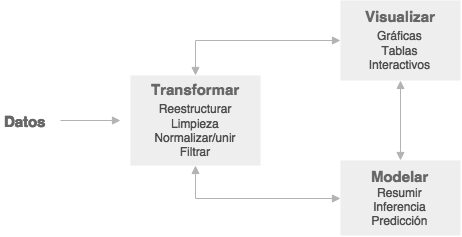
\includegraphics{imagenes/analisis.png}

Es importante la forma en que nos movemos dentro de estos procesos en el
análisis de datos y en este curso buscamos dar herramientas para facilitar
cumplir los siguientes principios:

\begin{enumerate}
\def\labelenumi{\arabic{enumi}.}
\item
  \textbf{Reproducibilidad}. Debe ser posible reproducir el análisis en todos sus
  pasos, en cualquier momento.
\item
  \textbf{Claridad}. Los pasos del análisis deben estar documentados apropiadamente,
  de manera que las decisiones importantes puedan ser entendidas y explicadas
  claramente.
\end{enumerate}

Dedicaremos las primeras sesiones a aprender herramientas básicas para poder
movernos agilmente a lo largo de las etapas de análisis utilizando R y nos
enfocaremos en los paquetes que forman parte del
\href{http://tidyverse.org/}{tidyverse}.

\hypertarget{paquetes-y-el-tidyverse}{%
\subsection*{Paquetes y el Tidyverse}\label{paquetes-y-el-tidyverse}}
\addcontentsline{toc}{subsection}{Paquetes y el Tidyverse}

La mejor manera de usar R para análisis de datos es aprovechando la gran
cantidad de paquetes que aportan funcionalidad adicional. Desde
Rstudio podemos instalar paquetes (Tools - \textgreater{} Install packages o usar la
función \texttt{install.packages("nombre\_paquete")}). Una vez instalados, podemos
cargarlos a nuestra sesión de R mediante \texttt{library}. Por ejemplo, para cargar el
paquete \texttt{readr} hacemos:

\begin{Shaded}
\begin{Highlighting}[]
\CommentTok{\# print(read\_csv)}
\CommentTok{\# Error in print(read\_csv) : object \textquotesingle{}read\_csv\textquotesingle{} not found}
\FunctionTok{library}\NormalTok{(tidyverse)}
\FunctionTok{print}\NormalTok{(read\_csv)}
\end{Highlighting}
\end{Shaded}

\begin{verbatim}
## function (file, col_names = TRUE, col_types = NULL, col_select = NULL, 
##     id = NULL, locale = default_locale(), na = c("", "NA"), quoted_na = TRUE, 
##     quote = "\"", comment = "", trim_ws = TRUE, skip = 0, n_max = Inf, 
##     guess_max = min(1000, n_max), name_repair = "unique", num_threads = readr_threads(), 
##     progress = show_progress(), show_col_types = should_show_types(), 
##     skip_empty_rows = TRUE, lazy = should_read_lazy()) 
## {
##     if (edition_first()) {
##         tokenizer <- tokenizer_csv(na = na, quoted_na = quoted_na, 
##             quote = quote, comment = comment, trim_ws = trim_ws, 
##             skip_empty_rows = skip_empty_rows)
##         return(read_delimited(file, tokenizer, col_names = col_names, 
##             col_types = col_types, locale = locale, skip = skip, 
##             skip_empty_rows = skip_empty_rows, comment = comment, 
##             n_max = n_max, guess_max = guess_max, progress = progress, 
##             show_col_types = show_col_types))
##     }
##     if (!missing(quoted_na)) {
##         lifecycle::deprecate_soft("2.0.0", "readr::read_csv(quoted_na = )")
##     }
##     vroom::vroom(file, delim = ",", col_names = col_names, col_types = col_types, 
##         col_select = {
##             {
##                 col_select
##             }
##         }, id = id, .name_repair = name_repair, skip = skip, 
##         n_max = n_max, na = na, quote = quote, comment = comment, 
##         skip_empty_rows = skip_empty_rows, trim_ws = trim_ws, 
##         escape_double = TRUE, escape_backslash = FALSE, locale = locale, 
##         guess_max = guess_max, show_col_types = show_col_types, 
##         progress = progress, altrep = lazy, num_threads = num_threads)
## }
## <bytecode: 0x7f812ff77f50>
## <environment: namespace:readr>
\end{verbatim}

\texttt{read\_csv} es una función que aporta el paquete \texttt{readr}, que a su vez está incluido en el
\emph{tidyverse}.

Los paquetes se instalan una sola vez, sin embargo, se deben cargar
(ejecutar \texttt{library(tidyverse)}) en cada sesión de R que los ocupemos.

En estas notas utilizaremos la colección de paquetes incluídos en el
\href{https://www.tidyverse.org/}{tidyverse}. Estos paquetes de R están
diseñados para ciencia de datos, y para funcionar juntos como parte de un flujo
de trabajo.

La siguiente imagen tomada de \href{https://rviews.rstudio.com/2017/06/08/what-is-the-tidyverse/}{Why the tidyverse} (Joseph
Rickert) indica que paquetes del tidyverse se utilizan para cada
etapa del análisis de datos.

\begin{Shaded}
\begin{Highlighting}[]
\NormalTok{knitr}\SpecialCharTok{::}\FunctionTok{include\_graphics}\NormalTok{(}\StringTok{"imagenes/tidyverse.png"}\NormalTok{)}
\end{Highlighting}
\end{Shaded}

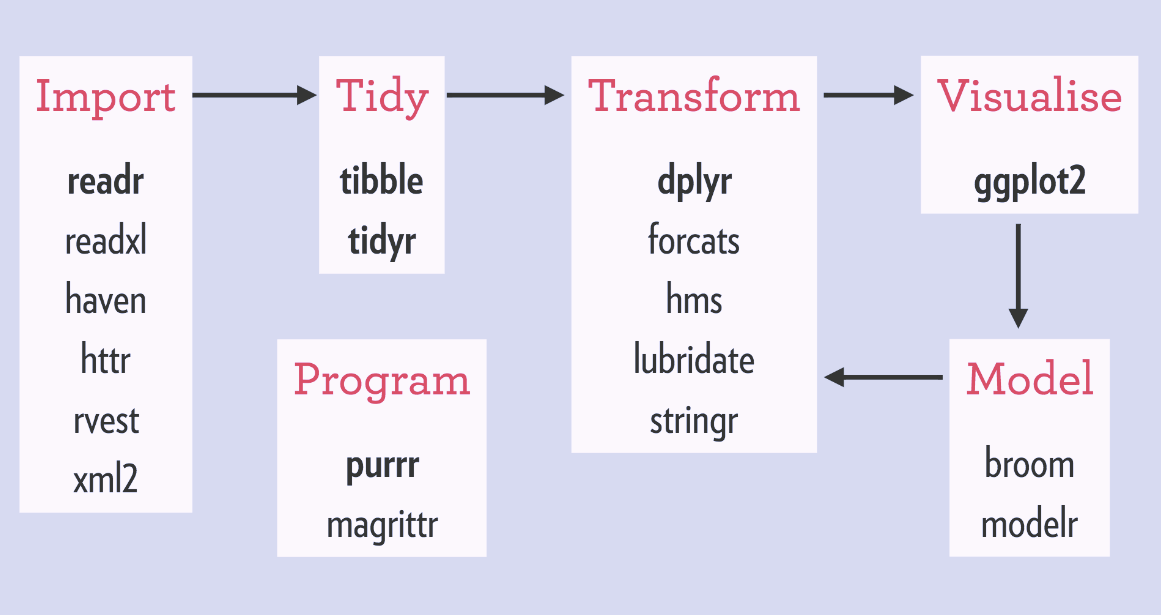
\includegraphics[width=16.12in]{imagenes/tidyverse}

\hypertarget{manipulaciuxf3n-y-agrupaciuxf3n-de-datos}{%
\chapter{Manipulación y agrupación de datos}\label{manipulaciuxf3n-y-agrupaciuxf3n-de-datos}}

\textbf{El material de la clase se puede descargar de \href{https://www.dropbox.com/s/gtxjn5xb39g2n09/02-manipulacion.zip?dl=0}{aquí}.}

En esta sección continuamos con la introducción a R para análisis de datos,
en particular mostraremos herramientas de manipulación y transformación de
datos. Trataremos los siguientes puntos:

\begin{itemize}
\item
  Estrategia separa-aplica-combina.
\item
  Reestructura de datos y el principio de los datos limpios.
\end{itemize}

Es sabido que limpieza y preparación de datos ocupan gran parte del tiempo del
análisis de datos (\href{http://onlinelibrary.wiley.com/book/10.1002/0471448354}{Dasu y Johnson, 2003}
y \href{https://www.nytimes.com/2014/08/18/technology/for-big-data-scientists-hurdle-to-insights-is-janitor-work.html?mcubz=0}{NYT's `Janitor Work' Is Key Hurdle to Insights}),
es por ello que vale la pena dedicar un tiempo a aprender técnicas que faciliten
estas tareas, y entender que estructura en los datos es más conveniente para
trabajar.

\hypertarget{transformaciuxf3n-de-datos}{%
\section{Transformación de datos}\label{transformaciuxf3n-de-datos}}

\hypertarget{datos-tidy}{%
\subsection*{Datos Tidy}\label{datos-tidy}}
\addcontentsline{toc}{subsection}{Datos Tidy}

Una base de datos tidy es una base de datos en la cuál:

\begin{itemize}
\tightlist
\item
  \textbf{Cada vararible que se medida debe estar en una columna.}
\item
  \textbf{Cada observación distinta de esa variable debe estar en una fila diferente.}
\item
  \textbf{Cada valor debe de estar en su propia celda}
\end{itemize}

En general, la forma en que representaríamos una base de datos tidy en R es usando un data frame.

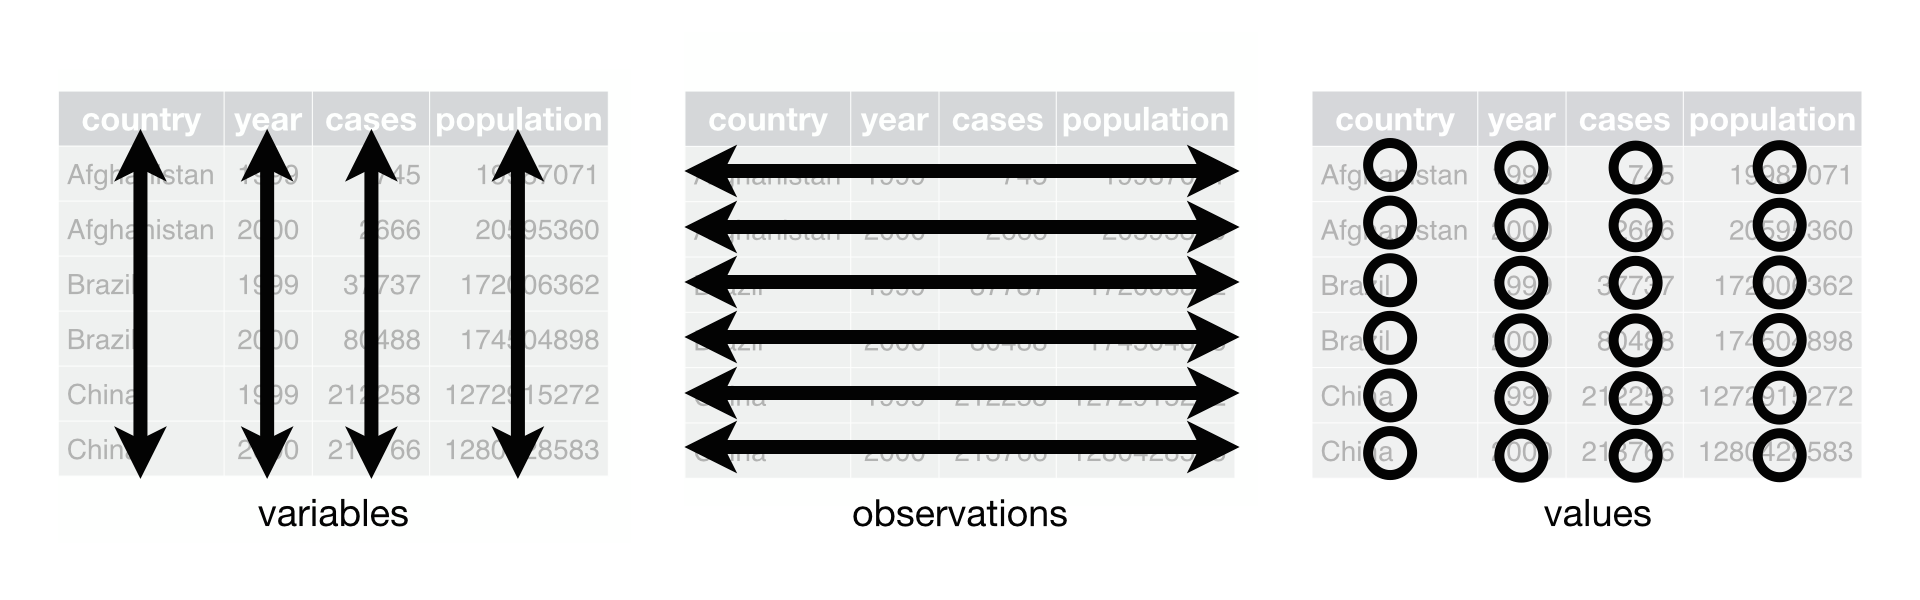
\includegraphics{imagenes/tidy.png}

Por ejemplo, los datos del Secretariado ejecutivo:

\begin{itemize}
\tightlist
\item
  Datos con la misma variable en diferentes columnas
\end{itemize}

\begin{verbatim}
#> # A tibble: 6 x 19
#>     Año Clave_Ent Entidad    Bien ~1 Tipo ~2 Subti~3 Modal~4 Enero Febrero Marzo
#>   <dbl>     <dbl> <chr>      <chr>   <chr>   <chr>   <chr>   <dbl>   <dbl> <dbl>
#> 1  2021         1 Aguascali~ La vid~ Homici~ Homici~ Con ar~     2       1     4
#> 2  2021         1 Aguascali~ La vid~ Homici~ Homici~ Con ar~     1       1     1
#> 3  2021         1 Aguascali~ La vid~ Homici~ Homici~ Con ot~     0       3     1
#> 4  2021         1 Aguascali~ La vid~ Homici~ Homici~ No esp~     0       0     0
#> 5  2021         1 Aguascali~ La vid~ Homici~ Homici~ Con ar~     0       0     0
#> 6  2021         1 Aguascali~ La vid~ Homici~ Homici~ Con ar~     0       0     0
#> # ... with 9 more variables: Abril <dbl>, Mayo <dbl>, Junio <dbl>, Julio <dbl>,
#> #   Agosto <dbl>, Septiembre <dbl>, Octubre <dbl>, Noviembre <dbl>,
#> #   Diciembre <dbl>, and abbreviated variable names
#> #   1: `Bien jurídico afectado`, 2: `Tipo de delito`, 3: `Subtipo de delito`,
#> #   4: Modalidad
\end{verbatim}

\begin{verbatim}
#> # A tibble: 20 x 9
#>      Año Clave_Ent Entidad        Bien j~1 Tipo ~2 Subti~3 Modal~4 mes   total~5
#>    <dbl>     <dbl> <chr>          <chr>    <chr>   <chr>   <chr>   <chr>   <dbl>
#>  1  2021         1 Aguascalientes La vida~ Homici~ Homici~ Con ar~ Enero       2
#>  2  2021         1 Aguascalientes La vida~ Homici~ Homici~ Con ar~ Enero       1
#>  3  2021         1 Aguascalientes La vida~ Homici~ Homici~ Con ot~ Enero       0
#>  4  2021         1 Aguascalientes La vida~ Homici~ Homici~ No esp~ Enero       0
#>  5  2021         1 Aguascalientes La vida~ Homici~ Homici~ Con ar~ Enero       0
#>  6  2021         1 Aguascalientes La vida~ Homici~ Homici~ Con ar~ Enero       0
#>  7  2021         1 Aguascalientes La vida~ Homici~ Homici~ En acc~ Enero       8
#>  8  2021         1 Aguascalientes La vida~ Homici~ Homici~ Con ot~ Enero       0
#>  9  2021         1 Aguascalientes La vida~ Homici~ Homici~ No esp~ Enero       0
#> 10  2021         1 Aguascalientes La vida~ Lesion~ Lesion~ Con ar~ Enero       5
#> 11  2021         1 Aguascalientes La vida~ Lesion~ Lesion~ Con ar~ Enero       7
#> 12  2021         1 Aguascalientes La vida~ Lesion~ Lesion~ Con ot~ Enero     160
#> 13  2021         1 Aguascalientes La vida~ Lesion~ Lesion~ No esp~ Enero      56
#> 14  2021         1 Aguascalientes La vida~ Lesion~ Lesion~ Con ar~ Enero       0
#> 15  2021         1 Aguascalientes La vida~ Lesion~ Lesion~ Con ar~ Enero       0
#> 16  2021         1 Aguascalientes La vida~ Lesion~ Lesion~ En acc~ Enero      59
#> 17  2021         1 Aguascalientes La vida~ Lesion~ Lesion~ Con ot~ Enero       0
#> 18  2021         1 Aguascalientes La vida~ Lesion~ Lesion~ No esp~ Enero      18
#> 19  2021         1 Aguascalientes La vida~ Femini~ Femini~ Con ar~ Enero       0
#> 20  2021         1 Aguascalientes La vida~ Femini~ Femini~ Con ar~ Enero       1
#> # ... with abbreviated variable names 1: `Bien jurídico afectado`,
#> #   2: `Tipo de delito`, 3: `Subtipo de delito`, 4: Modalidad, 5: total_delitos
\end{verbatim}

\begin{verbatim}
#> # A tibble: 40 x 33
#> # Groups:   Tipo de delito [40]
#>    Tipo de del~1 Aguas~2 Baja ~3 Baja ~4 Campe~5 Chiapas Chihu~6 Ciuda~7 Coahu~8
#>    <chr>           <dbl>   <dbl>   <dbl>   <dbl>   <dbl>   <dbl>   <dbl>   <dbl>
#>  1 Aborto              0       1       1       0       3       1       8       0
#>  2 Abuso de con~      50      29      12       0       4      60     302      52
#>  3 Abuso sexual        0      70      20       3      17     103     206      46
#>  4 Acoso sexual        0       0       8       0       7       0      86      15
#>  5 Allanamiento~      35     185       9       6       8      70      47      39
#>  6 Amenazas          227     324     102       5      26     248    1110     359
#>  7 Contra el me~       2       0       0       0       1      18      45       0
#>  8 Corrupción d~       5      50       3       0       3       5      21       3
#>  9 Daño a la pr~     317     576      85      12      67     656     697     459
#> 10 Delitos come~      47      69      18       0      10     134     307      13
#> # ... with 30 more rows, 24 more variables: Colima <dbl>, Durango <dbl>,
#> #   Guanajuato <dbl>, Guerrero <dbl>, Hidalgo <dbl>, Jalisco <dbl>,
#> #   México <dbl>, `Michoacán de Ocampo` <dbl>, Morelos <dbl>, Nayarit <dbl>,
#> #   `Nuevo León` <dbl>, Oaxaca <dbl>, Puebla <dbl>, Querétaro <dbl>,
#> #   `Quintana Roo` <dbl>, `San Luis Potosí` <dbl>, Sinaloa <dbl>, Sonora <dbl>,
#> #   Tabasco <dbl>, Tamaulipas <dbl>, Tlaxcala <dbl>,
#> #   `Veracruz de Ignacio de la Llave` <dbl>, Yucatán <dbl>, ...
\end{verbatim}

\begin{verbatim}
#>             estado municipio     mes total_delitos
#> 1 Estado de México      <NA>   Enero           143
#> 2 Estado de México      <NA> Febrero           234
#> 3 Estado de México      <NA>   Marzo           532
#> 4             <NA>    Toluca   Enero            12
#> 5             <NA>    Toluca Febrero             4
#> 6             <NA>    Toluca   Marzo            55
\end{verbatim}

\hypertarget{separa-aplica-combina-split-apply-combine}{%
\subsection*{\texorpdfstring{Separa-aplica-combina (\emph{split-apply-combine})}{Separa-aplica-combina (split-apply-combine)}}\label{separa-aplica-combina-split-apply-combine}}
\addcontentsline{toc}{subsection}{Separa-aplica-combina (\emph{split-apply-combine})}

Muchos problemas de análisis de datos involucran la aplicación de la estrategia
separa-aplica-combina \citep{plyr},
esta consiste en romper un problema en pedazos (de
acuerdo a una variable de interés), operar sobre cada subconjunto de manera
independiente (ej. calcular la media de cada grupo, ordenar observaciones por
grupo, estandarizar por grupo) y después unir los pedazos nuevamente. El
siguiente diagrama ejemplifiaca el paradigma de divide-aplica-combina:

\begin{itemize}
\tightlist
\item
  \textbf{Separa} la base de datos original.\\
\item
  \textbf{Aplica} funciones a cada subconjunto.\\
\item
  \textbf{Combina} los resultados en una nueva base de datos.
\end{itemize}

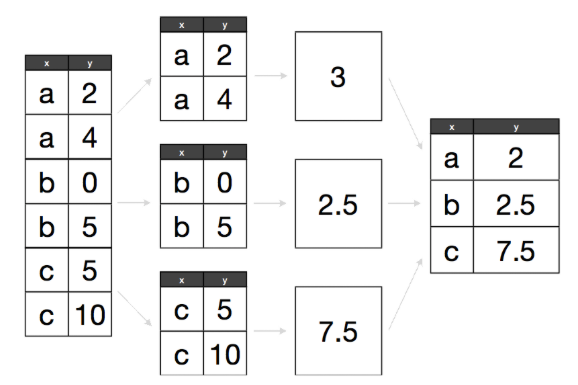
\includegraphics{imagenes/split-apply-combine.png}

Ahora, cuando pensamos como implementar la estrategia divide-aplica-combina es
natural pensar en iteraciones, por ejemplo utilizar un ciclo \texttt{for} para recorrer
cada grupo de interés y aplicar las funciones, sin embargo la aplicación de
ciclos \texttt{for} desemboca en código difícil de entender por lo que preferimos
trabajar con funciones creadas para estas tareas, usaremos el paquete
\texttt{dplyr} que además de ser más claro suele ser más veloz.

Estudiaremos las siguientes funciones:

\begin{itemize}
\tightlist
\item
  \textbf{filter}: obten un subconjunto de las filas de acuerdo a un criterio.
\item
  \textbf{select}: selecciona columnas de acuerdo al nombre
\item
  \textbf{arrange}: reordena las filas
\item
  \textbf{mutate}: agrega nuevas variables
\item
  \textbf{summarise}: reduce variables a valores (crear nuevas bases de datos con
  resúmenes de variables de la base original)
\end{itemize}

Estas funciones trabajan de manera similar, el primer argumento que reciben
es un \emph{data frame}, los argumentos que siguen
indican que operación se va a efectuar y el resultado es un nuevo \emph{data frame}.

Adicionalmente, se pueden usar con \textbf{group\_by} que cambia el dominio de cada
función, pasando de operar en el conjunto de datos completos a operar en
grupos, esto lo veremos más adelante.

\hypertarget{ejemplos-y-lectura-de-datos}{%
\subsection*{Ejemplos y lectura de datos}\label{ejemplos-y-lectura-de-datos}}
\addcontentsline{toc}{subsection}{Ejemplos y lectura de datos}

En esta sección trabajaremos con bases de datos de vuelos del aeropuerto de
Houston. Comenzamos importando los datos a R.

Para leer los datos usamos funciones del paquete \texttt{readr} que forma parte del
\texttt{tidyverse}, notemos que si estamos usando RStudio podemos generar los comandos
de lectura de datos usando la opción \emph{Import Dataset} en la ventana de
\emph{Environment}.

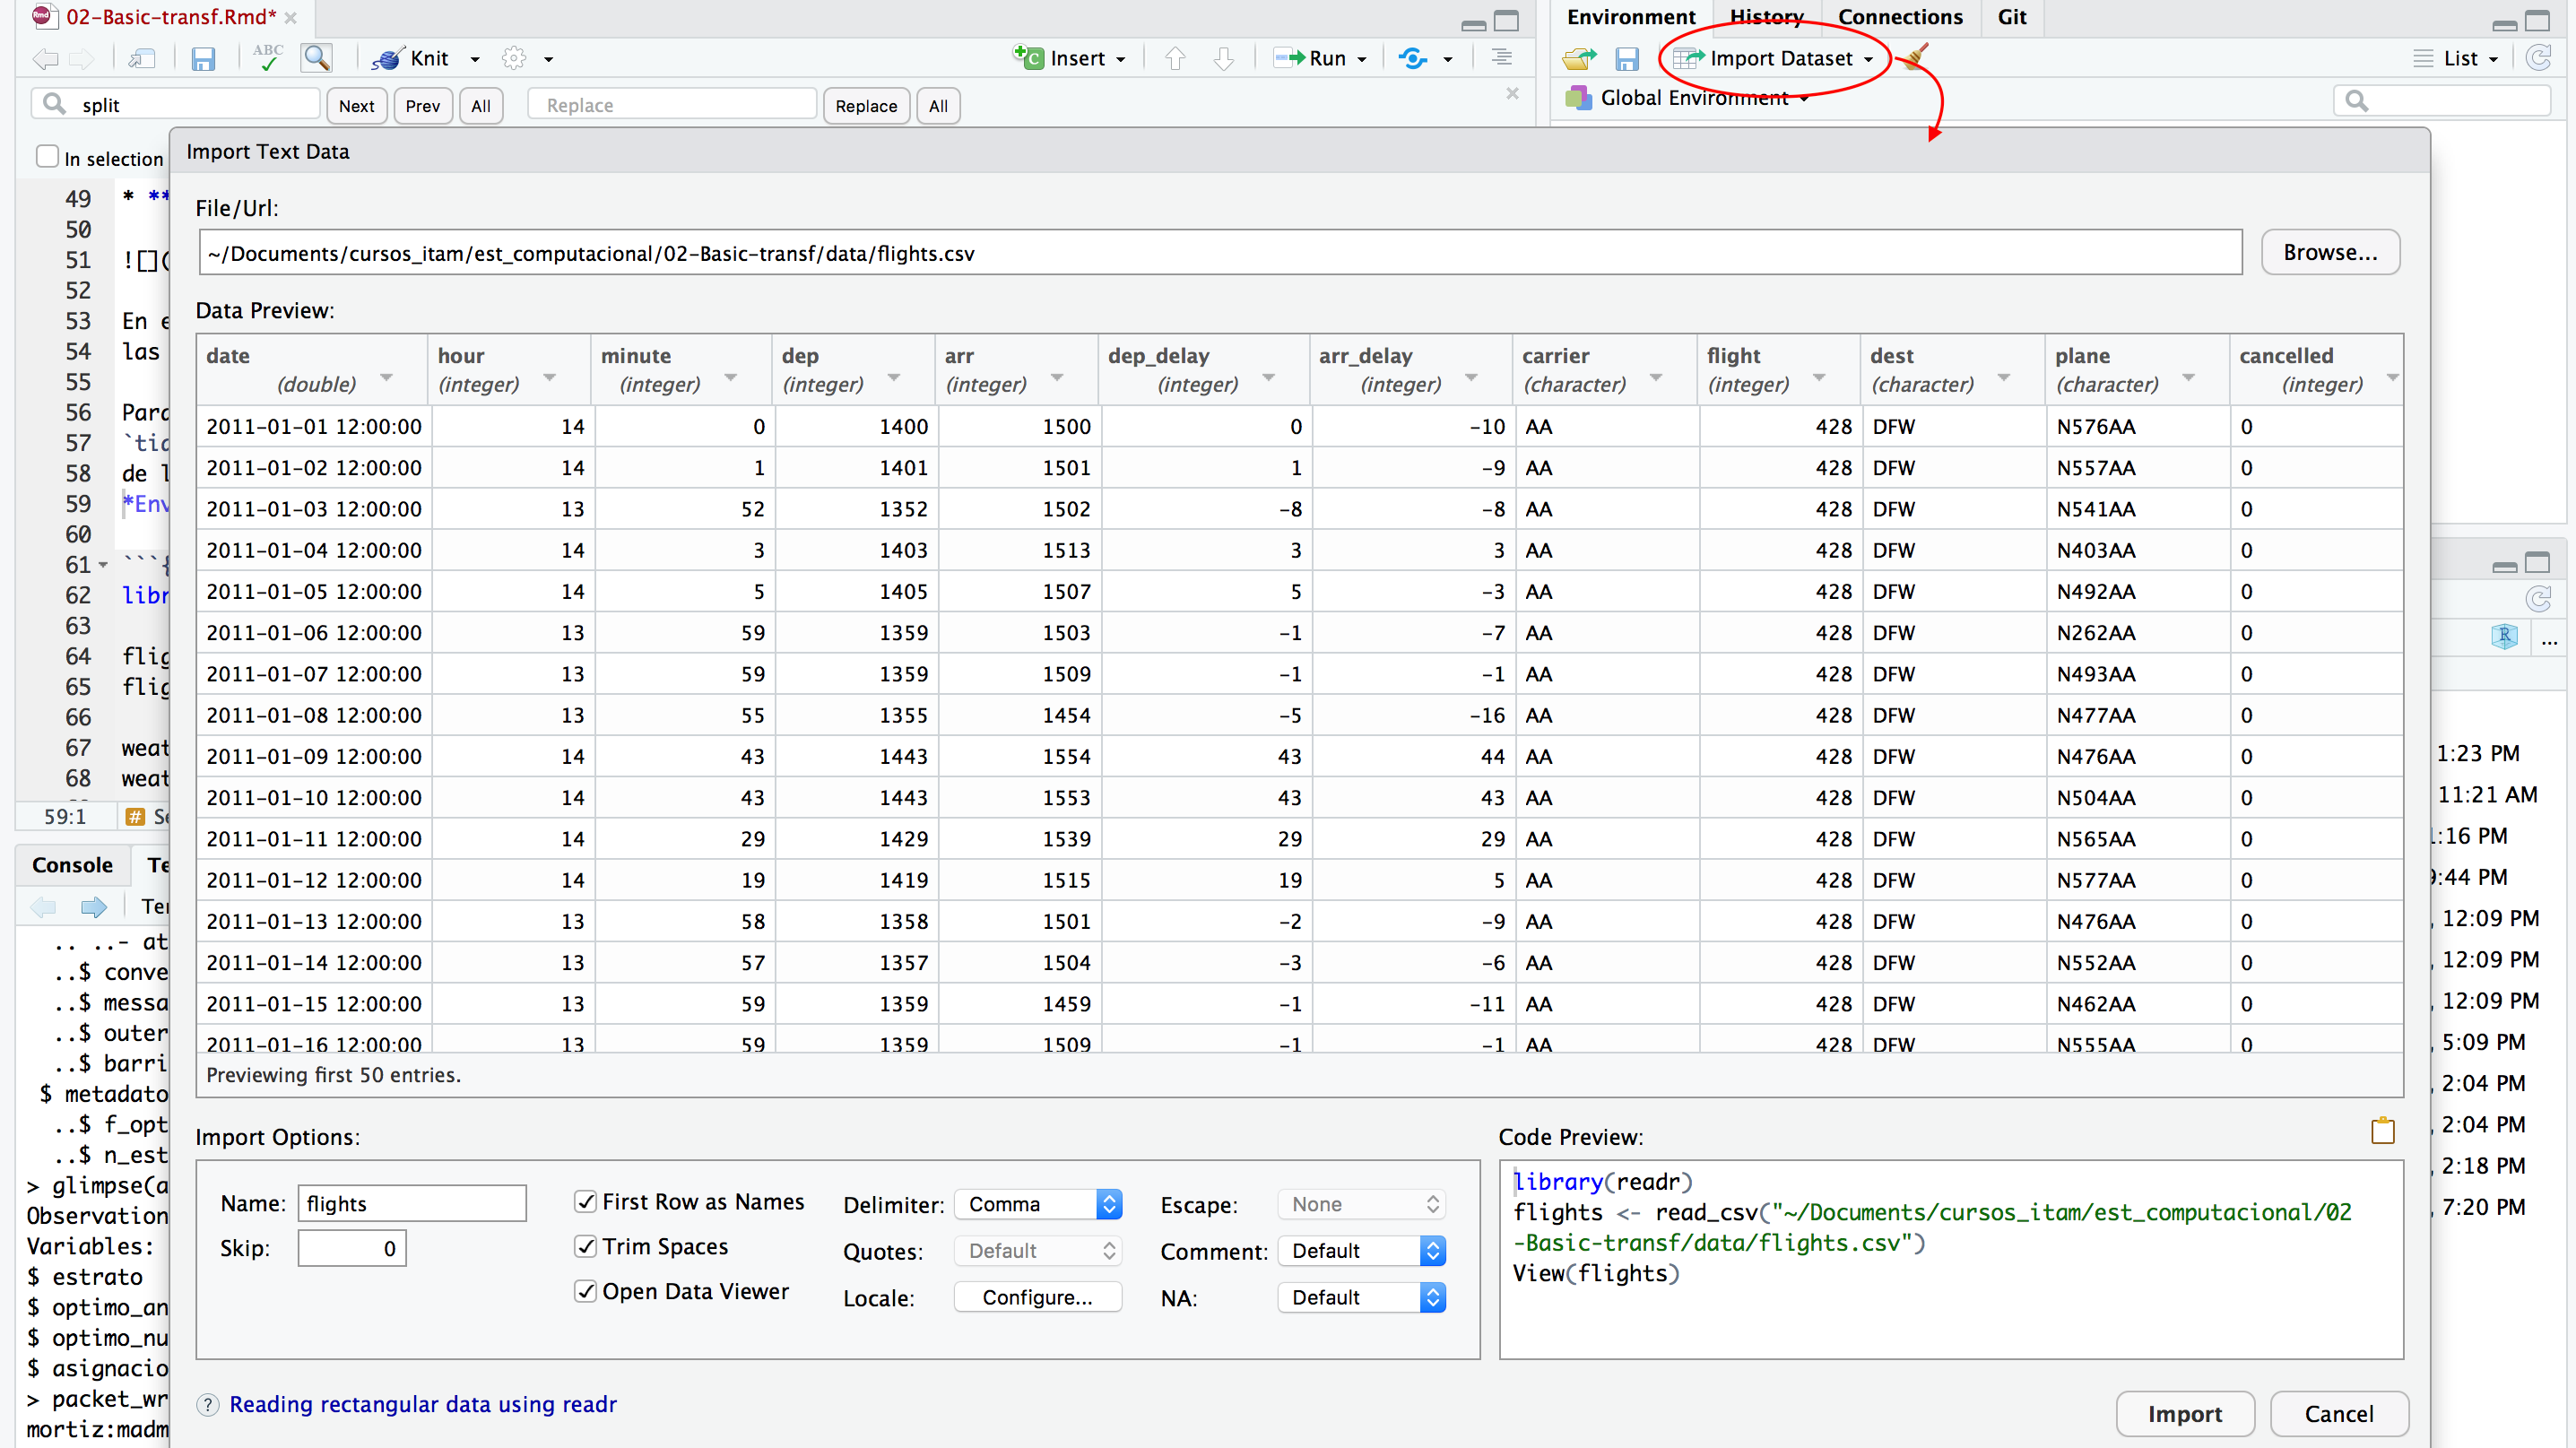
\includegraphics{imagenes/importar_RStudio.png}

Si usamos la opción de importar datos usando la funcionalidad \emph{point-and-click}
de RStudio, es importante copiar los comandos al script de R para no perder
reproducibilidad.

\begin{Shaded}
\begin{Highlighting}[]
\FunctionTok{library}\NormalTok{(tidyverse)}
\NormalTok{flights }\OtherTok{\textless{}{-}} \FunctionTok{read\_csv}\NormalTok{(}\StringTok{"data/flights.csv"}\NormalTok{)}
\CommentTok{\#\textgreater{} Rows: 227496 Columns: 14}
\CommentTok{\#\textgreater{} {-}{-} Column specification {-}{-}{-}{-}{-}{-}{-}{-}{-}{-}{-}{-}{-}{-}{-}{-}{-}{-}{-}{-}{-}{-}{-}{-}{-}{-}{-}{-}{-}{-}{-}{-}{-}{-}{-}{-}{-}{-}{-}{-}{-}{-}{-}{-}{-}{-}{-}{-}{-}{-}{-}{-}{-}{-}{-}{-}}
\CommentTok{\#\textgreater{} Delimiter: ","}
\CommentTok{\#\textgreater{} chr   (3): carrier, dest, plane}
\CommentTok{\#\textgreater{} dbl  (10): hour, minute, dep, arr, dep\_delay, arr\_delay, flight, cancelled, ...}
\CommentTok{\#\textgreater{} dttm  (1): date}
\CommentTok{\#\textgreater{} }
\CommentTok{\#\textgreater{} i Use \textasciigrave{}spec()\textasciigrave{} to retrieve the full column specification for this data.}
\CommentTok{\#\textgreater{} i Specify the column types or set \textasciigrave{}show\_col\_types = FALSE\textasciigrave{} to quiet this message.}
\NormalTok{flights}
\CommentTok{\#\textgreater{} \# A tibble: 227,496 x 14}
\CommentTok{\#\textgreater{}    date                 hour minute   dep   arr dep\_delay arr\_d\textasciitilde{}1 carrier flight}
\CommentTok{\#\textgreater{}    \textless{}dttm\textgreater{}              \textless{}dbl\textgreater{}  \textless{}dbl\textgreater{} \textless{}dbl\textgreater{} \textless{}dbl\textgreater{}     \textless{}dbl\textgreater{}   \textless{}dbl\textgreater{} \textless{}chr\textgreater{}    \textless{}dbl\textgreater{}}
\CommentTok{\#\textgreater{}  1 2011{-}01{-}01 12:00:00    14      0  1400  1500         0     {-}10 AA         428}
\CommentTok{\#\textgreater{}  2 2011{-}01{-}02 12:00:00    14      1  1401  1501         1      {-}9 AA         428}
\CommentTok{\#\textgreater{}  3 2011{-}01{-}03 12:00:00    13     52  1352  1502        {-}8      {-}8 AA         428}
\CommentTok{\#\textgreater{}  4 2011{-}01{-}04 12:00:00    14      3  1403  1513         3       3 AA         428}
\CommentTok{\#\textgreater{}  5 2011{-}01{-}05 12:00:00    14      5  1405  1507         5      {-}3 AA         428}
\CommentTok{\#\textgreater{}  6 2011{-}01{-}06 12:00:00    13     59  1359  1503        {-}1      {-}7 AA         428}
\CommentTok{\#\textgreater{}  7 2011{-}01{-}07 12:00:00    13     59  1359  1509        {-}1      {-}1 AA         428}
\CommentTok{\#\textgreater{}  8 2011{-}01{-}08 12:00:00    13     55  1355  1454        {-}5     {-}16 AA         428}
\CommentTok{\#\textgreater{}  9 2011{-}01{-}09 12:00:00    14     43  1443  1554        43      44 AA         428}
\CommentTok{\#\textgreater{} 10 2011{-}01{-}10 12:00:00    14     43  1443  1553        43      43 AA         428}
\CommentTok{\#\textgreater{} \# ... with 227,486 more rows, 5 more variables: dest \textless{}chr\textgreater{}, plane \textless{}chr\textgreater{},}
\CommentTok{\#\textgreater{} \#   cancelled \textless{}dbl\textgreater{}, time \textless{}dbl\textgreater{}, dist \textless{}dbl\textgreater{}, and abbreviated variable name}
\CommentTok{\#\textgreater{} \#   1: arr\_delay}
\NormalTok{weather }\OtherTok{\textless{}{-}} \FunctionTok{read\_csv}\NormalTok{(}\StringTok{"data/weather.csv"}\NormalTok{)}
\CommentTok{\#\textgreater{} Rows: 8723 Columns: 14}
\CommentTok{\#\textgreater{} {-}{-} Column specification {-}{-}{-}{-}{-}{-}{-}{-}{-}{-}{-}{-}{-}{-}{-}{-}{-}{-}{-}{-}{-}{-}{-}{-}{-}{-}{-}{-}{-}{-}{-}{-}{-}{-}{-}{-}{-}{-}{-}{-}{-}{-}{-}{-}{-}{-}{-}{-}{-}{-}{-}{-}{-}{-}{-}{-}}
\CommentTok{\#\textgreater{} Delimiter: ","}
\CommentTok{\#\textgreater{} chr   (3): wind\_dir, conditions, events}
\CommentTok{\#\textgreater{} dbl  (10): hour, temp, dew\_point, humidity, pressure, visibility, wind\_dir2,...}
\CommentTok{\#\textgreater{} date  (1): date}
\CommentTok{\#\textgreater{} }
\CommentTok{\#\textgreater{} i Use \textasciigrave{}spec()\textasciigrave{} to retrieve the full column specification for this data.}
\CommentTok{\#\textgreater{} i Specify the column types or set \textasciigrave{}show\_col\_types = FALSE\textasciigrave{} to quiet this message.}
\NormalTok{weather }
\CommentTok{\#\textgreater{} \# A tibble: 8,723 x 14}
\CommentTok{\#\textgreater{}    date        hour  temp dew\_point humidity pressure visibility wind\_\textasciitilde{}1 wind\_\textasciitilde{}2}
\CommentTok{\#\textgreater{}    \textless{}date\textgreater{}     \textless{}dbl\textgreater{} \textless{}dbl\textgreater{}     \textless{}dbl\textgreater{}    \textless{}dbl\textgreater{}    \textless{}dbl\textgreater{}      \textless{}dbl\textgreater{} \textless{}chr\textgreater{}     \textless{}dbl\textgreater{}}
\CommentTok{\#\textgreater{}  1 2011{-}01{-}01     0  59        28.9       32     29.9         10 NNE          20}
\CommentTok{\#\textgreater{}  2 2011{-}01{-}01     1  57.2      28.4       33     29.9         10 NNE          20}
\CommentTok{\#\textgreater{}  3 2011{-}01{-}01     2  55.4      28.4       36     29.9         10 NNW         340}
\CommentTok{\#\textgreater{}  4 2011{-}01{-}01     3  53.6      28.4       38     29.9         10 North       350}
\CommentTok{\#\textgreater{}  5 2011{-}01{-}01     4  NA        NA         NA     30.0         10 NNW         340}
\CommentTok{\#\textgreater{}  6 2011{-}01{-}01     5  NA        NA         NA     30.0         10 North       350}
\CommentTok{\#\textgreater{}  7 2011{-}01{-}01     6  53.1      17.1       24     30.0         10 North       360}
\CommentTok{\#\textgreater{}  8 2011{-}01{-}01     7  53.1      16         23     30.1         10 North        10}
\CommentTok{\#\textgreater{}  9 2011{-}01{-}01     8  54        18         24     30.1         10 North        10}
\CommentTok{\#\textgreater{} 10 2011{-}01{-}01     9  55.4      17.6       23     30.1         10 NNE          20}
\CommentTok{\#\textgreater{} \# ... with 8,713 more rows, 5 more variables: wind\_speed \textless{}dbl\textgreater{},}
\CommentTok{\#\textgreater{} \#   gust\_speed \textless{}dbl\textgreater{}, precip \textless{}dbl\textgreater{}, conditions \textless{}chr\textgreater{}, events \textless{}chr\textgreater{}, and}
\CommentTok{\#\textgreater{} \#   abbreviated variable names 1: wind\_dir, 2: wind\_dir2}
\NormalTok{planes }\OtherTok{\textless{}{-}} \FunctionTok{read\_csv}\NormalTok{(}\StringTok{"data/planes.csv"}\NormalTok{)}
\CommentTok{\#\textgreater{} Rows: 2853 Columns: 9}
\CommentTok{\#\textgreater{} {-}{-} Column specification {-}{-}{-}{-}{-}{-}{-}{-}{-}{-}{-}{-}{-}{-}{-}{-}{-}{-}{-}{-}{-}{-}{-}{-}{-}{-}{-}{-}{-}{-}{-}{-}{-}{-}{-}{-}{-}{-}{-}{-}{-}{-}{-}{-}{-}{-}{-}{-}{-}{-}{-}{-}{-}{-}{-}{-}}
\CommentTok{\#\textgreater{} Delimiter: ","}
\CommentTok{\#\textgreater{} chr (5): plane, mfr, model, engine, type}
\CommentTok{\#\textgreater{} dbl (4): year, no.eng, no.seats, speed}
\CommentTok{\#\textgreater{} }
\CommentTok{\#\textgreater{} i Use \textasciigrave{}spec()\textasciigrave{} to retrieve the full column specification for this data.}
\CommentTok{\#\textgreater{} i Specify the column types or set \textasciigrave{}show\_col\_types = FALSE\textasciigrave{} to quiet this message.}
\NormalTok{planes}
\CommentTok{\#\textgreater{} \# A tibble: 2,853 x 9}
\CommentTok{\#\textgreater{}    plane   year mfr               model        no.eng no.se\textasciitilde{}1 speed engine type }
\CommentTok{\#\textgreater{}    \textless{}chr\textgreater{}  \textless{}dbl\textgreater{} \textless{}chr\textgreater{}             \textless{}chr\textgreater{}         \textless{}dbl\textgreater{}   \textless{}dbl\textgreater{} \textless{}dbl\textgreater{} \textless{}chr\textgreater{}  \textless{}chr\textgreater{}}
\CommentTok{\#\textgreater{}  1 N576AA  1991 MCDONNELL DOUGLAS DC{-}9{-}82(MD{-}\textasciitilde{}      2     172    NA Turbo\textasciitilde{} Fixe\textasciitilde{}}
\CommentTok{\#\textgreater{}  2 N557AA  1993 MARZ BARRY        KITFOX IV         1       2    NA Recip\textasciitilde{} Fixe\textasciitilde{}}
\CommentTok{\#\textgreater{}  3 N403AA  1974 RAVEN             S55A             NA       1    60 None   Ball\textasciitilde{}}
\CommentTok{\#\textgreater{}  4 N492AA  1989 MCDONNELL DOUGLAS DC{-}9{-}82(MD{-}\textasciitilde{}      2     172    NA Turbo\textasciitilde{} Fixe\textasciitilde{}}
\CommentTok{\#\textgreater{}  5 N262AA  1985 MCDONNELL DOUGLAS DC{-}9{-}82(MD{-}\textasciitilde{}      2     172    NA Turbo\textasciitilde{} Fixe\textasciitilde{}}
\CommentTok{\#\textgreater{}  6 N493AA  1989 MCDONNELL DOUGLAS DC{-}9{-}82(MD{-}\textasciitilde{}      2     172    NA Turbo\textasciitilde{} Fixe\textasciitilde{}}
\CommentTok{\#\textgreater{}  7 N477AA  1988 MCDONNELL DOUGLAS DC{-}9{-}82(MD{-}\textasciitilde{}      2     172    NA Turbo\textasciitilde{} Fixe\textasciitilde{}}
\CommentTok{\#\textgreater{}  8 N476AA  1988 MCDONNELL DOUGLAS DC{-}9{-}82(MD{-}\textasciitilde{}      2     172    NA Turbo\textasciitilde{} Fixe\textasciitilde{}}
\CommentTok{\#\textgreater{}  9 N504AA    NA AUTHIER ANTHONY P TIERRA II         1       2    NA Recip\textasciitilde{} Fixe\textasciitilde{}}
\CommentTok{\#\textgreater{} 10 N565AA  1987 MCDONNELL DOUGLAS DC{-}9{-}83(MD{-}\textasciitilde{}      2     172    NA Turbo\textasciitilde{} Fixe\textasciitilde{}}
\CommentTok{\#\textgreater{} \# ... with 2,843 more rows, and abbreviated variable name 1: no.seats}
\NormalTok{airports }\OtherTok{\textless{}{-}} \FunctionTok{read\_csv}\NormalTok{(}\StringTok{"data/airports.csv"}\NormalTok{)}
\CommentTok{\#\textgreater{} Rows: 3376 Columns: 7}
\CommentTok{\#\textgreater{} {-}{-} Column specification {-}{-}{-}{-}{-}{-}{-}{-}{-}{-}{-}{-}{-}{-}{-}{-}{-}{-}{-}{-}{-}{-}{-}{-}{-}{-}{-}{-}{-}{-}{-}{-}{-}{-}{-}{-}{-}{-}{-}{-}{-}{-}{-}{-}{-}{-}{-}{-}{-}{-}{-}{-}{-}{-}{-}{-}}
\CommentTok{\#\textgreater{} Delimiter: ","}
\CommentTok{\#\textgreater{} chr (5): iata, airport, city, state, country}
\CommentTok{\#\textgreater{} dbl (2): lat, long}
\CommentTok{\#\textgreater{} }
\CommentTok{\#\textgreater{} i Use \textasciigrave{}spec()\textasciigrave{} to retrieve the full column specification for this data.}
\CommentTok{\#\textgreater{} i Specify the column types or set \textasciigrave{}show\_col\_types = FALSE\textasciigrave{} to quiet this message.}
\NormalTok{airports}
\CommentTok{\#\textgreater{} \# A tibble: 3,376 x 7}
\CommentTok{\#\textgreater{}    iata  airport              city             state country   lat   long}
\CommentTok{\#\textgreater{}    \textless{}chr\textgreater{} \textless{}chr\textgreater{}                \textless{}chr\textgreater{}            \textless{}chr\textgreater{} \textless{}chr\textgreater{}   \textless{}dbl\textgreater{}  \textless{}dbl\textgreater{}}
\CommentTok{\#\textgreater{}  1 00M   Thigpen              Bay Springs      MS    USA      32.0  {-}89.2}
\CommentTok{\#\textgreater{}  2 00R   Livingston Municipal Livingston       TX    USA      30.7  {-}95.0}
\CommentTok{\#\textgreater{}  3 00V   Meadow Lake          Colorado Springs CO    USA      38.9 {-}105. }
\CommentTok{\#\textgreater{}  4 01G   Perry{-}Warsaw         Perry            NY    USA      42.7  {-}78.1}
\CommentTok{\#\textgreater{}  5 01J   Hilliard Airpark     Hilliard         FL    USA      30.7  {-}81.9}
\CommentTok{\#\textgreater{}  6 01M   Tishomingo County    Belmont          MS    USA      34.5  {-}88.2}
\CommentTok{\#\textgreater{}  7 02A   Gragg{-}Wade           Clanton          AL    USA      32.9  {-}86.6}
\CommentTok{\#\textgreater{}  8 02C   Capitol              Brookfield       WI    USA      43.1  {-}88.2}
\CommentTok{\#\textgreater{}  9 02G   Columbiana County    East Liverpool   OH    USA      40.7  {-}80.6}
\CommentTok{\#\textgreater{} 10 03D   Memphis Memorial     Memphis          MO    USA      40.4  {-}92.2}
\CommentTok{\#\textgreater{} \# ... with 3,366 more rows}
\end{Highlighting}
\end{Shaded}

\hypertarget{filtrar}{%
\subsection*{Filtrar}\label{filtrar}}
\addcontentsline{toc}{subsection}{Filtrar}

Creamos una base de datos de juguete para mostrar el funcionamiento de cada
instrucción:

\begin{Shaded}
\begin{Highlighting}[]
\NormalTok{df\_ej }\OtherTok{\textless{}{-}} \FunctionTok{tibble}\NormalTok{(}\AttributeTok{genero =} \FunctionTok{c}\NormalTok{(}\StringTok{"mujer"}\NormalTok{, }\StringTok{"hombre"}\NormalTok{, }\StringTok{"mujer"}\NormalTok{, }\StringTok{"mujer"}\NormalTok{, }\StringTok{"hombre"}\NormalTok{), }
  \AttributeTok{estatura =} \FunctionTok{c}\NormalTok{(}\FloatTok{1.65}\NormalTok{, }\FloatTok{1.80}\NormalTok{, }\FloatTok{1.70}\NormalTok{, }\FloatTok{1.60}\NormalTok{, }\FloatTok{1.67}\NormalTok{))}
\NormalTok{df\_ej}
\CommentTok{\#\textgreater{} \# A tibble: 5 x 2}
\CommentTok{\#\textgreater{}   genero estatura}
\CommentTok{\#\textgreater{}   \textless{}chr\textgreater{}     \textless{}dbl\textgreater{}}
\CommentTok{\#\textgreater{} 1 mujer      1.65}
\CommentTok{\#\textgreater{} 2 hombre     1.8 }
\CommentTok{\#\textgreater{} 3 mujer      1.7 }
\CommentTok{\#\textgreater{} 4 mujer      1.6 }
\CommentTok{\#\textgreater{} 5 hombre     1.67}
\end{Highlighting}
\end{Shaded}

El primer argumento de \texttt{filter()} es el nombre del \emph{data frame}, los subsecuentes
son las expresiones que indican que filas filtrar.

\begin{Shaded}
\begin{Highlighting}[]
\FunctionTok{filter}\NormalTok{(df\_ej, genero }\SpecialCharTok{==} \StringTok{"mujer"}\NormalTok{)}
\CommentTok{\#\textgreater{} \# A tibble: 3 x 2}
\CommentTok{\#\textgreater{}   genero estatura}
\CommentTok{\#\textgreater{}   \textless{}chr\textgreater{}     \textless{}dbl\textgreater{}}
\CommentTok{\#\textgreater{} 1 mujer      1.65}
\CommentTok{\#\textgreater{} 2 mujer      1.7 }
\CommentTok{\#\textgreater{} 3 mujer      1.6}
\FunctionTok{filter}\NormalTok{(df\_ej, estatura }\SpecialCharTok{\textgreater{}} \FloatTok{1.65} \SpecialCharTok{\&}\NormalTok{ estatura }\SpecialCharTok{\textless{}} \FloatTok{1.75}\NormalTok{)}
\CommentTok{\#\textgreater{} \# A tibble: 2 x 2}
\CommentTok{\#\textgreater{}   genero estatura}
\CommentTok{\#\textgreater{}   \textless{}chr\textgreater{}     \textless{}dbl\textgreater{}}
\CommentTok{\#\textgreater{} 1 mujer      1.7 }
\CommentTok{\#\textgreater{} 2 hombre     1.67}
\end{Highlighting}
\end{Shaded}

Algunos operadores importantes para filtrar son:

\begin{Shaded}
\begin{Highlighting}[]
\NormalTok{x }\SpecialCharTok{\textgreater{}} \DecValTok{1}
\NormalTok{x }\SpecialCharTok{\textgreater{}=} \DecValTok{1}
\NormalTok{x }\SpecialCharTok{\textless{}} \DecValTok{1}
\NormalTok{x }\SpecialCharTok{\textless{}=} \DecValTok{1}
\NormalTok{x }\SpecialCharTok{!=} \DecValTok{1}
\NormalTok{x }\SpecialCharTok{==} \DecValTok{1}
\NormalTok{x }\SpecialCharTok{\%in\%} \FunctionTok{c}\NormalTok{(}\StringTok{"a"}\NormalTok{, }\StringTok{"b"}\NormalTok{)}
\end{Highlighting}
\end{Shaded}

Debemos tener cuidado al usar \texttt{==}

\begin{Shaded}
\begin{Highlighting}[]
\FunctionTok{sqrt}\NormalTok{(}\DecValTok{2}\NormalTok{) }\SpecialCharTok{\^{}} \DecValTok{2} \SpecialCharTok{==} \DecValTok{2}
\CommentTok{\#\textgreater{} [1] FALSE}
\DecValTok{1}\SpecialCharTok{/}\DecValTok{49} \SpecialCharTok{*} \DecValTok{49} \SpecialCharTok{==} \DecValTok{1}
\CommentTok{\#\textgreater{} [1] FALSE}
\end{Highlighting}
\end{Shaded}

Los resultados de arriba se deben a que las computadoras
usan aritmética de precisión finita:

\begin{Shaded}
\begin{Highlighting}[]
\FunctionTok{print}\NormalTok{(}\DecValTok{1}\SpecialCharTok{/}\DecValTok{49} \SpecialCharTok{*} \DecValTok{49}\NormalTok{, }\AttributeTok{digits =} \DecValTok{20}\NormalTok{)}
\CommentTok{\#\textgreater{} [1] 0.99999999999999988898}
\end{Highlighting}
\end{Shaded}

Para estos casos es útil usar la función \texttt{near()}

\begin{Shaded}
\begin{Highlighting}[]
\FunctionTok{near}\NormalTok{(}\FunctionTok{sqrt}\NormalTok{(}\DecValTok{2}\NormalTok{) }\SpecialCharTok{\^{}} \DecValTok{2}\NormalTok{,  }\DecValTok{2}\NormalTok{)}
\CommentTok{\#\textgreater{} [1] TRUE}
\FunctionTok{near}\NormalTok{(}\DecValTok{1} \SpecialCharTok{/} \DecValTok{49} \SpecialCharTok{*} \DecValTok{49}\NormalTok{, }\DecValTok{1}\NormalTok{)}
\CommentTok{\#\textgreater{} [1] TRUE}
\end{Highlighting}
\end{Shaded}

Los operadores booleanos también son convenientes para
filtrar:

\begin{Shaded}
\begin{Highlighting}[]
\CommentTok{\# Conjuntos}
\NormalTok{a }\SpecialCharTok{|}\NormalTok{ b}
\NormalTok{a }\SpecialCharTok{\&}\NormalTok{ b}
\NormalTok{a }\SpecialCharTok{\&} \SpecialCharTok{!}\NormalTok{b}
\FunctionTok{xor}\NormalTok{(a, b)}
\end{Highlighting}
\end{Shaded}

El siguiente esquema nos ayuda a entender que hace cada operación:

\begin{Shaded}
\begin{Highlighting}[]
\NormalTok{knitr}\SpecialCharTok{::}\FunctionTok{include\_graphics}\NormalTok{(}\StringTok{"imagenes/transform{-}logical.png"}\NormalTok{)}
\end{Highlighting}
\end{Shaded}

\begin{center}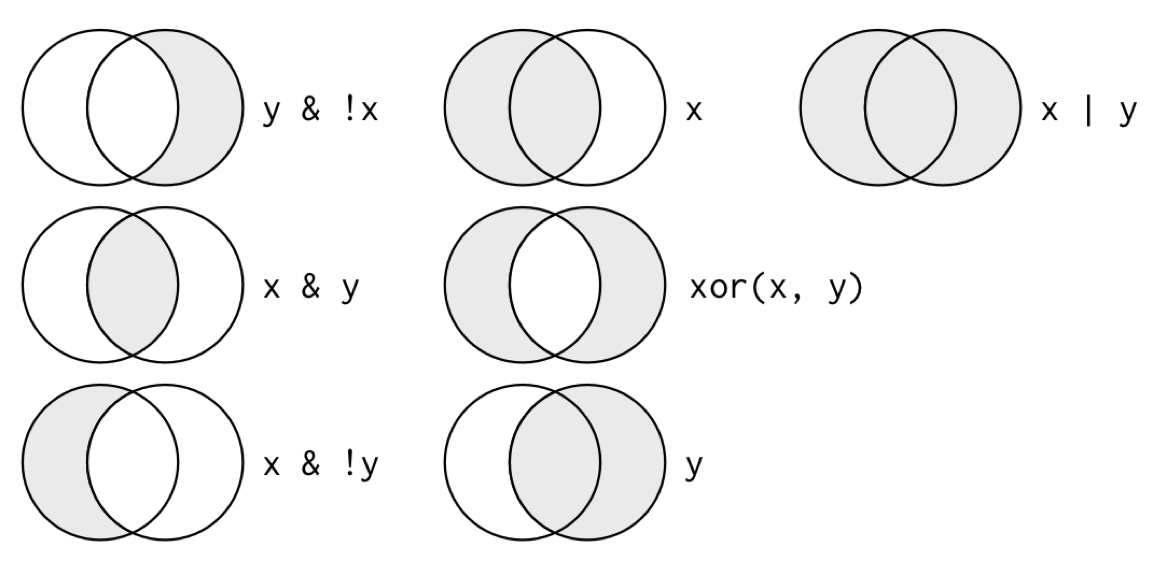
\includegraphics[width=16.08in]{imagenes/transform-logical} \end{center}


\includegraphics{imagenes/manicule2.jpg} Encuentra todos los vuelos hacia SFO ó OAK.

~~~~~~~~~~~ Los vuelos
con un retraso mayor a una hora.

~~~~~~~~~~~ En los que
el retraso de llegada es más del doble que el retraso de salida.

Un caso común es cuando se desea eliminar los datos con faltantes en una o más
columnas de las tablas de datos, en R los datos faltantes se expresan como \texttt{NA},
para eliminar los faltantes en la variable \texttt{dep\_delay} resulta natural escribir:

\begin{Shaded}
\begin{Highlighting}[]
\FunctionTok{filter}\NormalTok{(flights, dep\_delay }\SpecialCharTok{!=} \ConstantTok{NA}\NormalTok{)}
\CommentTok{\#\textgreater{} \# A tibble: 0 x 14}
\CommentTok{\#\textgreater{} \# ... with 14 variables: date \textless{}dttm\textgreater{}, hour \textless{}dbl\textgreater{}, minute \textless{}dbl\textgreater{}, dep \textless{}dbl\textgreater{},}
\CommentTok{\#\textgreater{} \#   arr \textless{}dbl\textgreater{}, dep\_delay \textless{}dbl\textgreater{}, arr\_delay \textless{}dbl\textgreater{}, carrier \textless{}chr\textgreater{}, flight \textless{}dbl\textgreater{},}
\CommentTok{\#\textgreater{} \#   dest \textless{}chr\textgreater{}, plane \textless{}chr\textgreater{}, cancelled \textless{}dbl\textgreater{}, time \textless{}dbl\textgreater{}, dist \textless{}dbl\textgreater{}}
\end{Highlighting}
\end{Shaded}

que nos devuelve una tabla vacía, sin embargo, si hay faltantes en esta
variable. El problema resulta de usar el operador \texttt{!=}, pensemos ¿qué regresan
las siguientes expresiones?

\begin{Shaded}
\begin{Highlighting}[]
\DecValTok{5} \SpecialCharTok{+} \ConstantTok{NA}
\ConstantTok{NA} \SpecialCharTok{/} \DecValTok{2}
\FunctionTok{sum}\NormalTok{(}\FunctionTok{c}\NormalTok{(}\DecValTok{5}\NormalTok{, }\DecValTok{4}\NormalTok{, }\ConstantTok{NA}\NormalTok{))}
\FunctionTok{mean}\NormalTok{(}\FunctionTok{c}\NormalTok{(}\DecValTok{5}\NormalTok{, }\DecValTok{4}\NormalTok{,  }\ConstantTok{NA}\NormalTok{))}
\ConstantTok{NA} \SpecialCharTok{\textless{}} \DecValTok{3}
\ConstantTok{NA} \SpecialCharTok{==} \DecValTok{3}
\ConstantTok{NA} \SpecialCharTok{==} \ConstantTok{NA}
\end{Highlighting}
\end{Shaded}

Las expresiones anteriores regresan \texttt{NA}, el hecho que la media de un vector
que incluye NAs o su suma regrese \texttt{NA}s se debe a que el default en R es
propagar los valores faltantes, esto es, si deconozco el valor de una de las
componentes de un vector, también desconozco la suma del mismo; sin embargo,
muchas funciones tienen un argumento \emph{na.rm} para removerlos,

\begin{Shaded}
\begin{Highlighting}[]
\FunctionTok{sum}\NormalTok{(}\FunctionTok{c}\NormalTok{(}\DecValTok{5}\NormalTok{, }\DecValTok{4}\NormalTok{, }\ConstantTok{NA}\NormalTok{), }\AttributeTok{na.rm =} \ConstantTok{TRUE}\NormalTok{)}
\CommentTok{\#\textgreater{} [1] 9}
\FunctionTok{mean}\NormalTok{(}\FunctionTok{c}\NormalTok{(}\DecValTok{5}\NormalTok{, }\DecValTok{4}\NormalTok{, }\ConstantTok{NA}\NormalTok{), }\AttributeTok{na.rm =} \ConstantTok{TRUE}\NormalTok{)}
\CommentTok{\#\textgreater{} [1] 4.5}
\end{Highlighting}
\end{Shaded}

Aún queda pendiente, como filtrarlos en una tabla, para esto veamos que el
manejo de datos faltantes en R utiliza una lógica ternaria (como SQL):

\begin{Shaded}
\begin{Highlighting}[]
\ConstantTok{NA} \SpecialCharTok{==} \ConstantTok{NA}
\CommentTok{\#\textgreater{} [1] NA}
\end{Highlighting}
\end{Shaded}

La expresión anterior puede resultar confusa, una manera de pensar en esto es
considerar los NA como \emph{no sé}, por ejemplo si no se la edad de Juan y no se la
edad de Esteban, la respuesta a ¿Juan tiene la misma edad que Esteban? es
\emph{no sé} (NA).

\begin{Shaded}
\begin{Highlighting}[]
\NormalTok{edad\_Juan }\OtherTok{\textless{}{-}} \ConstantTok{NA}
\NormalTok{edad\_Esteban }\OtherTok{\textless{}{-}} \ConstantTok{NA}
\NormalTok{edad\_Juan }\SpecialCharTok{==}\NormalTok{ edad\_Esteban}
\CommentTok{\#\textgreater{} [1] NA}
\NormalTok{edad\_Jose }\OtherTok{\textless{}{-}} \DecValTok{32}
\CommentTok{\# Juan es menor que José?}
\NormalTok{edad\_Juan }\SpecialCharTok{\textless{}}\NormalTok{ edad\_Jose}
\CommentTok{\#\textgreater{} [1] NA}
\end{Highlighting}
\end{Shaded}

Por tanto para determinar si un valor es faltante usamos la instrucción
\texttt{is.na()}.

\begin{Shaded}
\begin{Highlighting}[]
\FunctionTok{is.na}\NormalTok{(}\ConstantTok{NA}\NormalTok{)}
\CommentTok{\#\textgreater{} [1] TRUE}
\end{Highlighting}
\end{Shaded}

Y finalmente podemos filtrar con

\begin{Shaded}
\begin{Highlighting}[]
\FunctionTok{filter}\NormalTok{(flights, }\FunctionTok{is.na}\NormalTok{(dep\_delay))}
\end{Highlighting}
\end{Shaded}

\hypertarget{seleccionar}{%
\subsection*{Seleccionar}\label{seleccionar}}
\addcontentsline{toc}{subsection}{Seleccionar}

Elegir columnas de un conjunto de datos.

\begin{Shaded}
\begin{Highlighting}[]
\NormalTok{df\_ej}
\CommentTok{\#\textgreater{} \# A tibble: 5 x 2}
\CommentTok{\#\textgreater{}   genero estatura}
\CommentTok{\#\textgreater{}   \textless{}chr\textgreater{}     \textless{}dbl\textgreater{}}
\CommentTok{\#\textgreater{} 1 mujer      1.65}
\CommentTok{\#\textgreater{} 2 hombre     1.8 }
\CommentTok{\#\textgreater{} 3 mujer      1.7 }
\CommentTok{\#\textgreater{} 4 mujer      1.6 }
\CommentTok{\#\textgreater{} 5 hombre     1.67}
\FunctionTok{select}\NormalTok{(df\_ej, genero)}
\CommentTok{\#\textgreater{} \# A tibble: 5 x 1}
\CommentTok{\#\textgreater{}   genero}
\CommentTok{\#\textgreater{}   \textless{}chr\textgreater{} }
\CommentTok{\#\textgreater{} 1 mujer }
\CommentTok{\#\textgreater{} 2 hombre}
\CommentTok{\#\textgreater{} 3 mujer }
\CommentTok{\#\textgreater{} 4 mujer }
\CommentTok{\#\textgreater{} 5 hombre}
\FunctionTok{select}\NormalTok{(df\_ej, }\SpecialCharTok{{-}}\NormalTok{genero)}
\CommentTok{\#\textgreater{} \# A tibble: 5 x 1}
\CommentTok{\#\textgreater{}   estatura}
\CommentTok{\#\textgreater{}      \textless{}dbl\textgreater{}}
\CommentTok{\#\textgreater{} 1     1.65}
\CommentTok{\#\textgreater{} 2     1.8 }
\CommentTok{\#\textgreater{} 3     1.7 }
\CommentTok{\#\textgreater{} 4     1.6 }
\CommentTok{\#\textgreater{} 5     1.67}
\end{Highlighting}
\end{Shaded}

\begin{Shaded}
\begin{Highlighting}[]
\FunctionTok{select}\NormalTok{(df\_ej, }\FunctionTok{starts\_with}\NormalTok{(}\StringTok{"g"}\NormalTok{))}
\FunctionTok{select}\NormalTok{(df\_ej, }\FunctionTok{contains}\NormalTok{(}\StringTok{"g"}\NormalTok{))}
\end{Highlighting}
\end{Shaded}


\includegraphics{imagenes/manicule2.jpg} Ve la ayuda de select (\texttt{?select}) y escribe tres
maneras de seleccionar las variables de retraso (delay).

\hypertarget{ordenar}{%
\subsection*{Ordenar}\label{ordenar}}
\addcontentsline{toc}{subsection}{Ordenar}

Ordenar de acuerdo al valor de una o más variables:

\begin{Shaded}
\begin{Highlighting}[]
\FunctionTok{arrange}\NormalTok{(df\_ej, genero)}
\CommentTok{\#\textgreater{} \# A tibble: 5 x 2}
\CommentTok{\#\textgreater{}   genero estatura}
\CommentTok{\#\textgreater{}   \textless{}chr\textgreater{}     \textless{}dbl\textgreater{}}
\CommentTok{\#\textgreater{} 1 hombre     1.8 }
\CommentTok{\#\textgreater{} 2 hombre     1.67}
\CommentTok{\#\textgreater{} 3 mujer      1.65}
\CommentTok{\#\textgreater{} 4 mujer      1.7 }
\CommentTok{\#\textgreater{} 5 mujer      1.6}
\FunctionTok{arrange}\NormalTok{(df\_ej, }\FunctionTok{desc}\NormalTok{(estatura))}
\CommentTok{\#\textgreater{} \# A tibble: 5 x 2}
\CommentTok{\#\textgreater{}   genero estatura}
\CommentTok{\#\textgreater{}   \textless{}chr\textgreater{}     \textless{}dbl\textgreater{}}
\CommentTok{\#\textgreater{} 1 hombre     1.8 }
\CommentTok{\#\textgreater{} 2 mujer      1.7 }
\CommentTok{\#\textgreater{} 3 hombre     1.67}
\CommentTok{\#\textgreater{} 4 mujer      1.65}
\CommentTok{\#\textgreater{} 5 mujer      1.6}
\end{Highlighting}
\end{Shaded}


\includegraphics{imagenes/manicule2.jpg} Ordena los vuelos por fecha de salida y hora.

~~~~~~~~~~~ ¿Cuáles
son los vuelos con mayor retraso?

~~~~~~~~~~~ ¿Qué vuelos
\emph{ganaron} más tiempo en el aire?

\hypertarget{mutar}{%
\subsection*{Mutar}\label{mutar}}
\addcontentsline{toc}{subsection}{Mutar}

Mutar consiste en crear nuevas variables aplicando una función a columnas
existentes:

\begin{Shaded}
\begin{Highlighting}[]
\FunctionTok{mutate}\NormalTok{(df\_ej, }\AttributeTok{estatura\_cm =}\NormalTok{ estatura }\SpecialCharTok{*} \DecValTok{100}\NormalTok{) }
\CommentTok{\#\textgreater{} \# A tibble: 5 x 3}
\CommentTok{\#\textgreater{}   genero estatura estatura\_cm}
\CommentTok{\#\textgreater{}   \textless{}chr\textgreater{}     \textless{}dbl\textgreater{}       \textless{}dbl\textgreater{}}
\CommentTok{\#\textgreater{} 1 mujer      1.65         165}
\CommentTok{\#\textgreater{} 2 hombre     1.8          180}
\CommentTok{\#\textgreater{} 3 mujer      1.7          170}
\CommentTok{\#\textgreater{} 4 mujer      1.6          160}
\CommentTok{\#\textgreater{} 5 hombre     1.67         167}
\FunctionTok{mutate}\NormalTok{(df\_ej, }\AttributeTok{estatura\_cm =}\NormalTok{ estatura }\SpecialCharTok{*} \DecValTok{100}\NormalTok{, }\AttributeTok{estatura\_in =}\NormalTok{ estatura\_cm }\SpecialCharTok{*} \FloatTok{0.3937}\NormalTok{) }
\CommentTok{\#\textgreater{} \# A tibble: 5 x 4}
\CommentTok{\#\textgreater{}   genero estatura estatura\_cm estatura\_in}
\CommentTok{\#\textgreater{}   \textless{}chr\textgreater{}     \textless{}dbl\textgreater{}       \textless{}dbl\textgreater{}       \textless{}dbl\textgreater{}}
\CommentTok{\#\textgreater{} 1 mujer      1.65         165        65.0}
\CommentTok{\#\textgreater{} 2 hombre     1.8          180        70.9}
\CommentTok{\#\textgreater{} 3 mujer      1.7          170        66.9}
\CommentTok{\#\textgreater{} 4 mujer      1.6          160        63.0}
\CommentTok{\#\textgreater{} 5 hombre     1.67         167        65.7}
\end{Highlighting}
\end{Shaded}


\includegraphics{imagenes/manicule2.jpg} Calcula la velocidad en millas por hora a partir de
la variable tiempo y la distancia (en millas). ¿Quá vuelo fue el más rápido?

~~~~~~~~~~~ Crea una nueva
variable que muestre cuánto tiempo se ganó o perdió durante el vuelo.

Hay muchas funciones que podemos usar para crear nuevas variables con \texttt{mutate()}, éstas deben cumplir ser funciones vectorizadas, es decir, reciben un vector de valores y devuelven un vector de la misma dimensión.

\hypertarget{summarise-y-resuxfamenes-por-grupo}{%
\subsection*{Summarise y resúmenes por grupo}\label{summarise-y-resuxfamenes-por-grupo}}
\addcontentsline{toc}{subsection}{Summarise y resúmenes por grupo}

Summarise sirve para crear nuevas bases de datos con resúmenes o agregaciones de
los datos originales.

\begin{Shaded}
\begin{Highlighting}[]
\FunctionTok{summarise}\NormalTok{(df\_ej, }\AttributeTok{promedio =} \FunctionTok{mean}\NormalTok{(estatura))}
\CommentTok{\#\textgreater{} \# A tibble: 1 x 1}
\CommentTok{\#\textgreater{}   promedio}
\CommentTok{\#\textgreater{}      \textless{}dbl\textgreater{}}
\CommentTok{\#\textgreater{} 1     1.68}
\end{Highlighting}
\end{Shaded}

Podemos hacer resúmenes por grupo, primero creamos una base de datos agrupada:

\begin{Shaded}
\begin{Highlighting}[]
\NormalTok{by\_genero }\OtherTok{\textless{}{-}} \FunctionTok{group\_by}\NormalTok{(df\_ej, genero)}
\NormalTok{by\_genero}
\CommentTok{\#\textgreater{} \# A tibble: 5 x 2}
\CommentTok{\#\textgreater{} \# Groups:   genero [2]}
\CommentTok{\#\textgreater{}   genero estatura}
\CommentTok{\#\textgreater{}   \textless{}chr\textgreater{}     \textless{}dbl\textgreater{}}
\CommentTok{\#\textgreater{} 1 mujer      1.65}
\CommentTok{\#\textgreater{} 2 hombre     1.8 }
\CommentTok{\#\textgreater{} 3 mujer      1.7 }
\CommentTok{\#\textgreater{} 4 mujer      1.6 }
\CommentTok{\#\textgreater{} 5 hombre     1.67}
\end{Highlighting}
\end{Shaded}

y después operamos sobre cada grupo, creando un resumen a nivel grupo y uniendo
los subconjuntos en una base nueva:

\begin{Shaded}
\begin{Highlighting}[]
\FunctionTok{summarise}\NormalTok{(by\_genero, }\AttributeTok{promedio =} \FunctionTok{mean}\NormalTok{(estatura))}
\CommentTok{\#\textgreater{} \# A tibble: 2 x 2}
\CommentTok{\#\textgreater{}   genero promedio}
\CommentTok{\#\textgreater{}   \textless{}chr\textgreater{}     \textless{}dbl\textgreater{}}
\CommentTok{\#\textgreater{} 1 hombre     1.74}
\CommentTok{\#\textgreater{} 2 mujer      1.65}
\end{Highlighting}
\end{Shaded}


\includegraphics{imagenes/manicule2.jpg} Calcula el retraso promedio por fecha.

~~~~~~~~~~~ ¿Qué otros
resúmenes puedes hacer para explorar el retraso por fecha?

\begin{itemize}
\tightlist
\item
  Algunas funciones útiles con \emph{summarise} son min(x), median(x), max(x),
  quantile(x, p), n(), sum(x), sum(x \textgreater{} 1), mean(x \textgreater{} 1), sd(x).
\end{itemize}

\begin{Shaded}
\begin{Highlighting}[]
\NormalTok{flights}\SpecialCharTok{$}\NormalTok{date\_only }\OtherTok{\textless{}{-}} \FunctionTok{as.Date}\NormalTok{(flights}\SpecialCharTok{$}\NormalTok{date)}
\NormalTok{by\_date }\OtherTok{\textless{}{-}} \FunctionTok{group\_by}\NormalTok{(flights, date\_only)}
\NormalTok{no\_miss }\OtherTok{\textless{}{-}} \FunctionTok{filter}\NormalTok{(by\_date, }\SpecialCharTok{!}\FunctionTok{is.na}\NormalTok{(dep))}
\NormalTok{delays }\OtherTok{\textless{}{-}} \FunctionTok{summarise}\NormalTok{(no\_miss, }\AttributeTok{mean\_delay =} \FunctionTok{mean}\NormalTok{(dep\_delay), }\AttributeTok{n =} \FunctionTok{n}\NormalTok{())}
\end{Highlighting}
\end{Shaded}

\hypertarget{operador-pipeline}{%
\subsection*{Operador pipeline}\label{operador-pipeline}}
\addcontentsline{toc}{subsection}{Operador pipeline}

En R cuando uno hace varias operaciones es difícil leer y entender el código:

\begin{Shaded}
\begin{Highlighting}[]
\NormalTok{hourly\_delay }\OtherTok{\textless{}{-}} \FunctionTok{filter}\NormalTok{(}\FunctionTok{summarise}\NormalTok{(}\FunctionTok{group\_by}\NormalTok{(}\FunctionTok{filter}\NormalTok{(flights, }\SpecialCharTok{!}\FunctionTok{is.na}\NormalTok{(dep\_delay)), }
\NormalTok{  date\_only, hour), }\AttributeTok{delay =} \FunctionTok{mean}\NormalTok{(dep\_delay), }\AttributeTok{n =} \FunctionTok{n}\NormalTok{()), n }\SpecialCharTok{\textgreater{}} \DecValTok{10}\NormalTok{)}
\CommentTok{\#\textgreater{} \textasciigrave{}summarise()\textasciigrave{} has grouped output by \textquotesingle{}date\_only\textquotesingle{}. You can override using the}
\CommentTok{\#\textgreater{} \textasciigrave{}.groups\textasciigrave{} argument.}
\end{Highlighting}
\end{Shaded}

La dificultad radica en que usualmente los parámetros se asignan después del
nombre de la función usando (). El operador \emph{Forward Pipe} (\texttt{\%\textgreater{}\%)\ cambia\ este\ \ orden,\ de\ manera\ que\ un\ parámetro\ que\ precede\ a\ la\ función\ es\ enviado\ ("piped")\ \ a\ la\ función:}x \%\textgreater\% f(y)\texttt{se\ vuelve}f(x,y)\texttt{,}x \%\textgreater\% f(y) \%\textgreater\% g(z)\texttt{se\ vuelve}g(f(x, y), z)`. Es así que podemos reescribir el código para poder leer las
operaciones que vamos aplicando de izquierda a derecha
y de arriba hacia abajo.
Veamos como cambia el código anterior:

\begin{Shaded}
\begin{Highlighting}[]
\NormalTok{hourly\_delay }\OtherTok{\textless{}{-}}\NormalTok{ flights }\SpecialCharTok{\%\textgreater{}\%}
  \FunctionTok{filter}\NormalTok{(}\SpecialCharTok{!}\FunctionTok{is.na}\NormalTok{(dep\_delay)) }\SpecialCharTok{\%\textgreater{}\%}
  \FunctionTok{group\_by}\NormalTok{(date\_only, hour) }\SpecialCharTok{\%\textgreater{}\%}
  \FunctionTok{summarise}\NormalTok{(}\AttributeTok{delay =} \FunctionTok{mean}\NormalTok{(dep\_delay), }\AttributeTok{n =} \FunctionTok{n}\NormalTok{()) }\SpecialCharTok{\%\textgreater{}\%}
  \FunctionTok{filter}\NormalTok{(n }\SpecialCharTok{\textgreater{}} \DecValTok{10}\NormalTok{)}
\CommentTok{\#\textgreater{} \textasciigrave{}summarise()\textasciigrave{} has grouped output by \textquotesingle{}date\_only\textquotesingle{}. You can override using the}
\CommentTok{\#\textgreater{} \textasciigrave{}.groups\textasciigrave{} argument.}
\end{Highlighting}
\end{Shaded}

podemos leer \%\textgreater\% como ``\emph{después}''.


\includegraphics{imagenes/manicule2.jpg} ¿Qué destinos tienen el promedio de retrasos más
alto?

~~~~~~~~~~~ ¿Qué vuelos
(compañía + vuelo) ocurren diario?

~~~~~~~~~~~ En promedio,
¿Cómo varían a lo largo del día los retrasos de vuelos no cancelados? (pista: hour +
minute / 60)

\hypertarget{variables-por-grupo}{%
\subsection*{Variables por grupo}\label{variables-por-grupo}}
\addcontentsline{toc}{subsection}{Variables por grupo}

En ocasiones es conveniente crear variables por grupo, por ejemplo estandarizar
dentro de cada grupo z = (x - mean(x)) / sd(x).

Veamos un ejemplo:

\begin{Shaded}
\begin{Highlighting}[]
\NormalTok{planes }\OtherTok{\textless{}{-}}\NormalTok{ flights }\SpecialCharTok{\%\textgreater{}\%}
  \FunctionTok{filter}\NormalTok{(}\SpecialCharTok{!}\FunctionTok{is.na}\NormalTok{(arr\_delay)) }\SpecialCharTok{\%\textgreater{}\%}
  \FunctionTok{group\_by}\NormalTok{(plane) }\SpecialCharTok{\%\textgreater{}\%}
  \FunctionTok{filter}\NormalTok{(}\FunctionTok{n}\NormalTok{() }\SpecialCharTok{\textgreater{}} \DecValTok{30}\NormalTok{)}
\NormalTok{planes }\SpecialCharTok{\%\textgreater{}\%}
  \FunctionTok{mutate}\NormalTok{(}\AttributeTok{z\_delay =}
\NormalTok{    (arr\_delay }\SpecialCharTok{{-}} \FunctionTok{mean}\NormalTok{(arr\_delay)) }\SpecialCharTok{/} \FunctionTok{sd}\NormalTok{(arr\_delay)) }\SpecialCharTok{\%\textgreater{}\%}
  \FunctionTok{filter}\NormalTok{(z\_delay }\SpecialCharTok{\textgreater{}} \DecValTok{5}\NormalTok{)}
\CommentTok{\#\textgreater{} \# A tibble: 1,403 x 16}
\CommentTok{\#\textgreater{} \# Groups:   plane [856]}
\CommentTok{\#\textgreater{}    date                 hour minute   dep   arr dep\_delay arr\_d\textasciitilde{}1 carrier flight}
\CommentTok{\#\textgreater{}    \textless{}dttm\textgreater{}              \textless{}dbl\textgreater{}  \textless{}dbl\textgreater{} \textless{}dbl\textgreater{} \textless{}dbl\textgreater{}     \textless{}dbl\textgreater{}   \textless{}dbl\textgreater{} \textless{}chr\textgreater{}    \textless{}dbl\textgreater{}}
\CommentTok{\#\textgreater{}  1 2011{-}01{-}28 12:00:00    15     16  1516  1916       351     326 CO           1}
\CommentTok{\#\textgreater{}  2 2011{-}01{-}27 12:00:00    18     22  1822  1945       234     210 CO         137}
\CommentTok{\#\textgreater{}  3 2011{-}01{-}27 12:00:00    21     37  2137  2254       242     219 CO         150}
\CommentTok{\#\textgreater{}  4 2011{-}01{-}27 12:00:00     0     11    11   216       168     137 CO         209}
\CommentTok{\#\textgreater{}  5 2011{-}01{-}27 12:00:00    22     37  2237   153       227     208 CO         250}
\CommentTok{\#\textgreater{}  6 2011{-}01{-}27 12:00:00    21     28  2128   136       231     216 CO        1632}
\CommentTok{\#\textgreater{}  7 2011{-}01{-}26 12:00:00    11     46  1146  1633       171     193 CO         510}
\CommentTok{\#\textgreater{}  8 2011{-}01{-}26 12:00:00     9     49   949  1436       144     180 CO         776}
\CommentTok{\#\textgreater{}  9 2011{-}01{-}21 12:00:00    19     11  1911  2352        94     112 CO        1632}
\CommentTok{\#\textgreater{} 10 2011{-}01{-}20 12:00:00     6     35   635   807       780     775 CO          59}
\CommentTok{\#\textgreater{} \# ... with 1,393 more rows, 7 more variables: dest \textless{}chr\textgreater{}, plane \textless{}chr\textgreater{},}
\CommentTok{\#\textgreater{} \#   cancelled \textless{}dbl\textgreater{}, time \textless{}dbl\textgreater{}, dist \textless{}dbl\textgreater{}, date\_only \textless{}date\textgreater{}, z\_delay \textless{}dbl\textgreater{},}
\CommentTok{\#\textgreater{} \#   and abbreviated variable name 1: arr\_delay}
\end{Highlighting}
\end{Shaded}

\hypertarget{verbos-de-dos-tablas}{%
\subsection*{Verbos de dos tablas}\label{verbos-de-dos-tablas}}
\addcontentsline{toc}{subsection}{Verbos de dos tablas}

¿Cómo mostramos los retrasos de los vuelos en un mapa?

Para responder esta pregunta necesitamos unir la base de datos de vuelos
con la de aeropuertos.

\begin{Shaded}
\begin{Highlighting}[]
\NormalTok{location }\OtherTok{\textless{}{-}}\NormalTok{ airports }\SpecialCharTok{\%\textgreater{}\%}
  \FunctionTok{select}\NormalTok{(}\AttributeTok{dest =}\NormalTok{ iata, }\AttributeTok{name =}\NormalTok{ airport, lat, long)}
\NormalTok{flights }\SpecialCharTok{\%\textgreater{}\%}
    \FunctionTok{group\_by}\NormalTok{(dest) }\SpecialCharTok{\%\textgreater{}\%}
    \FunctionTok{filter}\NormalTok{(}\SpecialCharTok{!}\FunctionTok{is.na}\NormalTok{(arr\_delay)) }\SpecialCharTok{\%\textgreater{}\%}
    \FunctionTok{summarise}\NormalTok{(}
        \AttributeTok{arr\_delay =} \FunctionTok{mean}\NormalTok{(arr\_delay),}
        \AttributeTok{n =} \FunctionTok{n}\NormalTok{() ) }\SpecialCharTok{\%\textgreater{}\%}
        \FunctionTok{arrange}\NormalTok{(}\FunctionTok{desc}\NormalTok{(arr\_delay)) }\SpecialCharTok{\%\textgreater{}\%}
        \FunctionTok{left\_join}\NormalTok{(location)}
\CommentTok{\#\textgreater{} Joining, by = "dest"}
\CommentTok{\#\textgreater{} \# A tibble: 116 x 6}
\CommentTok{\#\textgreater{}    dest  arr\_delay     n name                                  lat   long}
\CommentTok{\#\textgreater{}    \textless{}chr\textgreater{}     \textless{}dbl\textgreater{} \textless{}int\textgreater{} \textless{}chr\textgreater{}                               \textless{}dbl\textgreater{}  \textless{}dbl\textgreater{}}
\CommentTok{\#\textgreater{}  1 ANC        26.1   124 Ted Stevens Anchorage International  61.2 {-}150. }
\CommentTok{\#\textgreater{}  2 CID        17.8   406 Eastern Iowa                         41.9  {-}91.7}
\CommentTok{\#\textgreater{}  3 DSM        16.0   634 Des Moines International             41.5  {-}93.7}
\CommentTok{\#\textgreater{}  4 SFO        14.9  2800 San Francisco International          37.6 {-}122. }
\CommentTok{\#\textgreater{}  5 BPT        14.3     3 Southeast Texas Regional             30.0  {-}94.0}
\CommentTok{\#\textgreater{}  6 GRR        13.7   665 Kent County International            42.9  {-}85.5}
\CommentTok{\#\textgreater{}  7 DAY        13.7   444 James M Cox Dayton Intl              39.9  {-}84.2}
\CommentTok{\#\textgreater{}  8 VPS        12.5   864 Eglin Air Force Base                 30.5  {-}86.5}
\CommentTok{\#\textgreater{}  9 ECP        12.4   720 \textless{}NA\textgreater{}                                 NA     NA  }
\CommentTok{\#\textgreater{} 10 SAV        12.3   851 Savannah International               32.1  {-}81.2}
\CommentTok{\#\textgreater{} \# ... with 106 more rows}
\end{Highlighting}
\end{Shaded}

Hay varias maneras de unir dos bases de datos y debemos pensar en el
obejtivo:

\begin{Shaded}
\begin{Highlighting}[]
\NormalTok{x }\OtherTok{\textless{}{-}} \FunctionTok{tibble}\NormalTok{(}\AttributeTok{name =} \FunctionTok{c}\NormalTok{(}\StringTok{"John"}\NormalTok{, }\StringTok{"Paul"}\NormalTok{, }\StringTok{"George"}\NormalTok{, }\StringTok{"Ringo"}\NormalTok{, }\StringTok{"Stuart"}\NormalTok{, }\StringTok{"Pete"}\NormalTok{),}
  \AttributeTok{instrument =} \FunctionTok{c}\NormalTok{(}\StringTok{"guitar"}\NormalTok{, }\StringTok{"bass"}\NormalTok{, }\StringTok{"guitar"}\NormalTok{, }\StringTok{"drums"}\NormalTok{, }\StringTok{"bass"}\NormalTok{,}
     \StringTok{"drums"}\NormalTok{))}
\NormalTok{y }\OtherTok{\textless{}{-}} \FunctionTok{tibble}\NormalTok{(}\AttributeTok{name =} \FunctionTok{c}\NormalTok{(}\StringTok{"John"}\NormalTok{, }\StringTok{"Paul"}\NormalTok{, }\StringTok{"George"}\NormalTok{, }\StringTok{"Ringo"}\NormalTok{, }\StringTok{"Brian"}\NormalTok{),}
  \AttributeTok{band =} \FunctionTok{c}\NormalTok{(}\StringTok{"TRUE"}\NormalTok{, }\StringTok{"TRUE"}\NormalTok{, }\StringTok{"TRUE"}\NormalTok{,  }\StringTok{"TRUE"}\NormalTok{, }\StringTok{"FALSE"}\NormalTok{))}
\NormalTok{x}
\CommentTok{\#\textgreater{} \# A tibble: 6 x 2}
\CommentTok{\#\textgreater{}   name   instrument}
\CommentTok{\#\textgreater{}   \textless{}chr\textgreater{}  \textless{}chr\textgreater{}     }
\CommentTok{\#\textgreater{} 1 John   guitar    }
\CommentTok{\#\textgreater{} 2 Paul   bass      }
\CommentTok{\#\textgreater{} 3 George guitar    }
\CommentTok{\#\textgreater{} 4 Ringo  drums     }
\CommentTok{\#\textgreater{} 5 Stuart bass      }
\CommentTok{\#\textgreater{} 6 Pete   drums}
\NormalTok{y}
\CommentTok{\#\textgreater{} \# A tibble: 5 x 2}
\CommentTok{\#\textgreater{}   name   band }
\CommentTok{\#\textgreater{}   \textless{}chr\textgreater{}  \textless{}chr\textgreater{}}
\CommentTok{\#\textgreater{} 1 John   TRUE }
\CommentTok{\#\textgreater{} 2 Paul   TRUE }
\CommentTok{\#\textgreater{} 3 George TRUE }
\CommentTok{\#\textgreater{} 4 Ringo  TRUE }
\CommentTok{\#\textgreater{} 5 Brian  FALSE}
\FunctionTok{inner\_join}\NormalTok{(x, y)}
\CommentTok{\#\textgreater{} Joining, by = "name"}
\CommentTok{\#\textgreater{} \# A tibble: 4 x 3}
\CommentTok{\#\textgreater{}   name   instrument band }
\CommentTok{\#\textgreater{}   \textless{}chr\textgreater{}  \textless{}chr\textgreater{}      \textless{}chr\textgreater{}}
\CommentTok{\#\textgreater{} 1 John   guitar     TRUE }
\CommentTok{\#\textgreater{} 2 Paul   bass       TRUE }
\CommentTok{\#\textgreater{} 3 George guitar     TRUE }
\CommentTok{\#\textgreater{} 4 Ringo  drums      TRUE}
\FunctionTok{left\_join}\NormalTok{(x, y)}
\CommentTok{\#\textgreater{} Joining, by = "name"}
\CommentTok{\#\textgreater{} \# A tibble: 6 x 3}
\CommentTok{\#\textgreater{}   name   instrument band }
\CommentTok{\#\textgreater{}   \textless{}chr\textgreater{}  \textless{}chr\textgreater{}      \textless{}chr\textgreater{}}
\CommentTok{\#\textgreater{} 1 John   guitar     TRUE }
\CommentTok{\#\textgreater{} 2 Paul   bass       TRUE }
\CommentTok{\#\textgreater{} 3 George guitar     TRUE }
\CommentTok{\#\textgreater{} 4 Ringo  drums      TRUE }
\CommentTok{\#\textgreater{} 5 Stuart bass       \textless{}NA\textgreater{} }
\CommentTok{\#\textgreater{} 6 Pete   drums      \textless{}NA\textgreater{}}
\FunctionTok{semi\_join}\NormalTok{(x, y)}
\CommentTok{\#\textgreater{} Joining, by = "name"}
\CommentTok{\#\textgreater{} \# A tibble: 4 x 2}
\CommentTok{\#\textgreater{}   name   instrument}
\CommentTok{\#\textgreater{}   \textless{}chr\textgreater{}  \textless{}chr\textgreater{}     }
\CommentTok{\#\textgreater{} 1 John   guitar    }
\CommentTok{\#\textgreater{} 2 Paul   bass      }
\CommentTok{\#\textgreater{} 3 George guitar    }
\CommentTok{\#\textgreater{} 4 Ringo  drums}
\FunctionTok{anti\_join}\NormalTok{(x, y)}
\CommentTok{\#\textgreater{} Joining, by = "name"}
\CommentTok{\#\textgreater{} \# A tibble: 2 x 2}
\CommentTok{\#\textgreater{}   name   instrument}
\CommentTok{\#\textgreater{}   \textless{}chr\textgreater{}  \textless{}chr\textgreater{}     }
\CommentTok{\#\textgreater{} 1 Stuart bass      }
\CommentTok{\#\textgreater{} 2 Pete   drums}
\end{Highlighting}
\end{Shaded}

Resumamos lo que observamos arriba:

\begin{longtable}[]{@{}ll@{}}
\toprule()
Tipo & Acción \\
\midrule()
\endhead
inner & Incluye únicamente las filas que aparecen tanto en x como en y \\
left & Incluye todas las filas en x y las filas de y que coincidan \\
semi & Incluye las filas de x que coincidan con y \\
anti & Incluye las filas de x que no coinciden con y \\
\bottomrule()
\end{longtable}

Ahora combinamos datos a nivel hora con condiciones climáticas, ¿cuál es el tipo
de unión adecuado?

\begin{Shaded}
\begin{Highlighting}[]
\NormalTok{hourly\_delay }\OtherTok{\textless{}{-}}\NormalTok{ flights }\SpecialCharTok{\%\textgreater{}\%}
  \FunctionTok{group\_by}\NormalTok{(date\_only, hour) }\SpecialCharTok{\%\textgreater{}\%}
  \FunctionTok{filter}\NormalTok{(}\SpecialCharTok{!}\FunctionTok{is.na}\NormalTok{(dep\_delay)) }\SpecialCharTok{\%\textgreater{}\%}
  \FunctionTok{summarise}\NormalTok{(}
    \AttributeTok{delay =} \FunctionTok{mean}\NormalTok{(dep\_delay),}
    \AttributeTok{n =} \FunctionTok{n}\NormalTok{() ) }\SpecialCharTok{\%\textgreater{}\%}
  \FunctionTok{filter}\NormalTok{(n }\SpecialCharTok{\textgreater{}} \DecValTok{10}\NormalTok{)}
\CommentTok{\#\textgreater{} \textasciigrave{}summarise()\textasciigrave{} has grouped output by \textquotesingle{}date\_only\textquotesingle{}. You can override using the}
\CommentTok{\#\textgreater{} \textasciigrave{}.groups\textasciigrave{} argument.}
\NormalTok{delay\_weather }\OtherTok{\textless{}{-}}\NormalTok{ hourly\_delay }\SpecialCharTok{\%\textgreater{}\%} \FunctionTok{left\_join}\NormalTok{(weather)}
\CommentTok{\#\textgreater{} Joining, by = "hour"}
\FunctionTok{arrange}\NormalTok{(delay\_weather, }\SpecialCharTok{{-}}\NormalTok{delay)}
\CommentTok{\#\textgreater{} \# A tibble: 2,091,842 x 17}
\CommentTok{\#\textgreater{} \# Groups:   date\_only [365]}
\CommentTok{\#\textgreater{}    date\_only   hour delay     n date        temp dew\_p\textasciitilde{}1 humid\textasciitilde{}2 press\textasciitilde{}3 visib\textasciitilde{}4}
\CommentTok{\#\textgreater{}    \textless{}date\textgreater{}     \textless{}dbl\textgreater{} \textless{}dbl\textgreater{} \textless{}int\textgreater{} \textless{}date\textgreater{}     \textless{}dbl\textgreater{}   \textless{}dbl\textgreater{}   \textless{}dbl\textgreater{}   \textless{}dbl\textgreater{}   \textless{}dbl\textgreater{}}
\CommentTok{\#\textgreater{}  1 2011{-}05{-}12    23  184.    33 2011{-}01{-}02  43      28.9      58    30.3      10}
\CommentTok{\#\textgreater{}  2 2011{-}05{-}12    23  184.    33 2011{-}01{-}03  39      27        62    30.3      10}
\CommentTok{\#\textgreater{}  3 2011{-}05{-}12    23  184.    33 2011{-}01{-}04  50      45        83    30.1      10}
\CommentTok{\#\textgreater{}  4 2011{-}05{-}12    23  184.    33 2011{-}01{-}05  62.6    60.8      94    30.0       5}
\CommentTok{\#\textgreater{}  5 2011{-}05{-}12    23  184.    33 2011{-}01{-}06  53.1    36        52    30.0      10}
\CommentTok{\#\textgreater{}  6 2011{-}05{-}12    23  184.    33 2011{-}01{-}07  46.9    36        66    30.0      10}
\CommentTok{\#\textgreater{}  7 2011{-}05{-}12    23  184.    33 2011{-}01{-}08  50      43        77    29.9      10}
\CommentTok{\#\textgreater{}  8 2011{-}05{-}12    23  184.    33 2011{-}01{-}09  53.1    30        41    29.9      10}
\CommentTok{\#\textgreater{}  9 2011{-}05{-}12    23  184.    33 2011{-}01{-}10  41      37        86    30.0      10}
\CommentTok{\#\textgreater{} 10 2011{-}05{-}12    23  184.    33 2011{-}01{-}11  39.9    32        73    30.3      10}
\CommentTok{\#\textgreater{} \# ... with 2,091,832 more rows, 7 more variables: wind\_dir \textless{}chr\textgreater{},}
\CommentTok{\#\textgreater{} \#   wind\_dir2 \textless{}dbl\textgreater{}, wind\_speed \textless{}dbl\textgreater{}, gust\_speed \textless{}dbl\textgreater{}, precip \textless{}dbl\textgreater{},}
\CommentTok{\#\textgreater{} \#   conditions \textless{}chr\textgreater{}, events \textless{}chr\textgreater{}, and abbreviated variable names}
\CommentTok{\#\textgreater{} \#   1: dew\_point, 2: humidity, 3: pressure, 4: visibility}
\end{Highlighting}
\end{Shaded}


\includegraphics{imagenes/manicule2.jpg} ¿Qué condiciones climáticas están asociadas
con retrasos en las salidas de Houston?

~~~~~~~~~~~ Explora
si los aviones más viejos están asociados a mayores retrasos, responde
con una gráfica.

\hypertarget{datos-limpios}{%
\section{Datos limpios}\label{datos-limpios}}

Una vez que importamos datos a R es conveniente limpiarlos, esto implica
almacenarlos de una manera consisistente que nos permita
enfocarnos en responder preguntas de los datos en lugar de estar luchando
con los datos. Entonces, \textbf{datos limpios} son datos que facilitan las tareas
del análisis de datos:

\begin{itemize}
\item
  \textbf{Visualización}: Resúmenes de datos usando gráficas, análisis exploratorio,
  o presentación de resultados.
\item
  \textbf{Manipulación}: Manipulación de variables como agregar, filtrar, reordenar,
  transformar.
\item
  \textbf{Modelación}: Ajustar modelos es sencillo si los datos están en la forma
  correcta.
\end{itemize}

Los principios de \emph{datos limpios} \citep{tidy}
proveen una manera estándar de organizar la información:

\begin{enumerate}
\def\labelenumi{\arabic{enumi}.}
\tightlist
\item
  Cada variable forma una columna.
\item
  Cada observación forma un renglón.
\item
  Cada tipo de unidad observacional forma una tabla.
\end{enumerate}

Vale la pena notar que los principios de los datos limpios se pueden ver como
teoría de algebra relacional para estadísticos, estós principios equivalen a
la tercera forma normal de Codd con enfoque en una sola tabla de datos en
lugar de muchas conectadas en bases de datos relacionales.

Veamos un ejemplo:

La mayor parte de las bases de datos en estadística tienen forma rectangular,
¿cuántas variables tiene la siguiente tabla?

\begin{longtable}[]{@{}lll@{}}
\toprule()
& tratamientoA & tratamientoB \\
\midrule()
\endhead
Juan Aguirre & - & 2 \\
Ana Bernal & 16 & 11 \\
José López & 3 & 1 \\
\bottomrule()
\end{longtable}

La tabla anterior también se puede estructurar de la siguiente manera:

\begin{longtable}[]{@{}llll@{}}
\toprule()
& Juan Aguirre & Ana Bernal & José López \\
\midrule()
\endhead
tratamientoA & - & 16 & 3 \\
tratamientoB & 2 & 11 & 1 \\
\bottomrule()
\end{longtable}

Si vemos los principios (cada variable forma una columna, cada observación
forma un renglón, cada tipo de unidad observacional forma una tabla), ¿las
tablas anteriores cumplen los principios?

Para responder la pregunta identifiquemos primero cuáles son las variables y
cuáles las observaciones de esta pequeña base. Las variables son:
persona/nombre, tratamiento y resultado. Entonces, siguiendo los principios de
\emph{datos limpios} obtenemos la siguiente estructura:

\begin{longtable}[]{@{}lll@{}}
\toprule()
nombre & tratamiento & resultado \\
\midrule()
\endhead
Juan Aguirre & a & - \\
Ana Bernal & a & 16 \\
José López & a & 3 \\
Juan Aguirre & b & 2 \\
Ana Bernal & b & 11 \\
José López & b & 1 \\
\bottomrule()
\end{longtable}

\hypertarget{limpieza-bases-de-datos}{%
\subsection*{Limpieza bases de datos}\label{limpieza-bases-de-datos}}
\addcontentsline{toc}{subsection}{Limpieza bases de datos}

Los principios de los datos limpios parecen obvios pero la mayor parte de los
datos no los cumplen debido a:

\begin{enumerate}
\def\labelenumi{\arabic{enumi}.}
\tightlist
\item
  La mayor parte de la gente no está familiarizada con los principios y es
  difícil derivarlos por uno mismo.\\
\item
  Los datos suelen estar organizados para facilitar otros aspectos que no son
  análisis, por ejemplo, la captura.
\end{enumerate}

Algunos de los problemas más comunes en las bases de datos que no están
\emph{limpias} son:

\begin{itemize}
\tightlist
\item
  Los encabezados de las columnas son valores y no nombres de variables.
\item
  Más de una variable por columna.
\item
  Las variables están organizadas tanto en filas como en columnas.
\item
  Más de un tipo de observación en una tabla.
\item
  Una misma unidad observacional está almacenada en múltiples tablas.
\end{itemize}

La mayor parte de estos problemas se pueden arreglar con pocas herramientas,
a continuación veremos como \emph{limpiar} datos usando 2 funciones del paquete
\texttt{tidyr}:

\begin{itemize}
\tightlist
\item
  \textbf{gather}: recibe múltiples columnas y las junta en pares de valores y
  nombres, convierte los datos anchos en largos.\\
\item
  \textbf{spread}: recibe 2 columnas y las separa, haciendo los datos más anchos.
\end{itemize}

Repasaremos los problemas más comunes que se encuentran en conjuntos de datos
sucios y mostraremos como se puede manipular la tabla de datos (usando las
funciones \emph{gather} y \emph{spread}) con el fin de estructurarla para que cumpla los
principios de datos limpios.

\hypertarget{los-encabezados-de-las-columanas-son-valores}{%
\subsection*{Los encabezados de las columanas son valores}\label{los-encabezados-de-las-columanas-son-valores}}
\addcontentsline{toc}{subsection}{Los encabezados de las columanas son valores}

Usaremos ejemplos para entender los conceptos más facilmente.
La primer base de datos está basada en una encuesta de \href{http://www.pewforum.org/2009/01/30/income-distribution-within-us-religious-groups/}{Pew Research} que
investiga la relación entre ingreso y afiliación religiosa.

¿Cuáles son las variables en estos datos?

\begin{Shaded}
\begin{Highlighting}[]
\FunctionTok{library}\NormalTok{(tidyverse)}
\NormalTok{pew }\OtherTok{\textless{}{-}} \FunctionTok{read\_delim}\NormalTok{(}\StringTok{"http://stat405.had.co.nz/data/pew.txt"}\NormalTok{, }\StringTok{"}\SpecialCharTok{\textbackslash{}t}\StringTok{"}\NormalTok{, }
  \AttributeTok{escape\_double =} \ConstantTok{FALSE}\NormalTok{, }\AttributeTok{trim\_ws =} \ConstantTok{TRUE}\NormalTok{)}
\CommentTok{\#\textgreater{} Rows: 18 Columns: 11}
\CommentTok{\#\textgreater{} {-}{-} Column specification {-}{-}{-}{-}{-}{-}{-}{-}{-}{-}{-}{-}{-}{-}{-}{-}{-}{-}{-}{-}{-}{-}{-}{-}{-}{-}{-}{-}{-}{-}{-}{-}{-}{-}{-}{-}{-}{-}{-}{-}{-}{-}{-}{-}{-}{-}{-}{-}{-}{-}{-}{-}{-}{-}{-}{-}}
\CommentTok{\#\textgreater{} Delimiter: "\textbackslash{}t"}
\CommentTok{\#\textgreater{} chr  (1): religion}
\CommentTok{\#\textgreater{} dbl (10): \textless{}$10k, $10{-}20k, $20{-}30k, $30{-}40k, $40{-}50k, $50{-}75k, $75{-}100k, $100...}
\CommentTok{\#\textgreater{} }
\CommentTok{\#\textgreater{} i Use \textasciigrave{}spec()\textasciigrave{} to retrieve the full column specification for this data.}
\CommentTok{\#\textgreater{} i Specify the column types or set \textasciigrave{}show\_col\_types = FALSE\textasciigrave{} to quiet this message.}
\NormalTok{pew}
\CommentTok{\#\textgreater{} \# A tibble: 18 x 11}
\CommentTok{\#\textgreater{}    religion      \textasciigrave{}\textless{}$10k\textasciigrave{} $10{-}2\textasciitilde{}1 $20{-}3\textasciitilde{}2 $30{-}4\textasciitilde{}3 $40{-}5\textasciitilde{}4 $50{-}7\textasciitilde{}5 $75{-}1\textasciitilde{}6 $100{-}\textasciitilde{}7}
\CommentTok{\#\textgreater{}    \textless{}chr\textgreater{}           \textless{}dbl\textgreater{}   \textless{}dbl\textgreater{}   \textless{}dbl\textgreater{}   \textless{}dbl\textgreater{}   \textless{}dbl\textgreater{}   \textless{}dbl\textgreater{}   \textless{}dbl\textgreater{}   \textless{}dbl\textgreater{}}
\CommentTok{\#\textgreater{}  1 Agnostic           27      34      60      81      76     137     122     109}
\CommentTok{\#\textgreater{}  2 Atheist            12      27      37      52      35      70      73      59}
\CommentTok{\#\textgreater{}  3 Buddhist           27      21      30      34      33      58      62      39}
\CommentTok{\#\textgreater{}  4 Catholic          418     617     732     670     638    1116     949     792}
\CommentTok{\#\textgreater{}  5 Don’t know/r\textasciitilde{}      15      14      15      11      10      35      21      17}
\CommentTok{\#\textgreater{}  6 Evangelical \textasciitilde{}     575     869    1064     982     881    1486     949     723}
\CommentTok{\#\textgreater{}  7 Hindu               1       9       7       9      11      34      47      48}
\CommentTok{\#\textgreater{}  8 Historically\textasciitilde{}     228     244     236     238     197     223     131      81}
\CommentTok{\#\textgreater{}  9 Jehovah\textquotesingle{}s Wi\textasciitilde{}      20      27      24      24      21      30      15      11}
\CommentTok{\#\textgreater{} 10 Jewish             19      19      25      25      30      95      69      87}
\CommentTok{\#\textgreater{} 11 Mainline Prot     289     495     619     655     651    1107     939     753}
\CommentTok{\#\textgreater{} 12 Mormon             29      40      48      51      56     112      85      49}
\CommentTok{\#\textgreater{} 13 Muslim              6       7       9      10       9      23      16       8}
\CommentTok{\#\textgreater{} 14 Orthodox           13      17      23      32      32      47      38      42}
\CommentTok{\#\textgreater{} 15 Other Christ\textasciitilde{}       9       7      11      13      13      14      18      14}
\CommentTok{\#\textgreater{} 16 Other Faiths       20      33      40      46      49      63      46      40}
\CommentTok{\#\textgreater{} 17 Other World \textasciitilde{}       5       2       3       4       2       7       3       4}
\CommentTok{\#\textgreater{} 18 Unaffiliated      217     299     374     365     341     528     407     321}
\CommentTok{\#\textgreater{} \# ... with 2 more variables: \textasciigrave{}\textgreater{}150k\textasciigrave{} \textless{}dbl\textgreater{}, \textasciigrave{}Don\textquotesingle{}t know/refused\textasciigrave{} \textless{}dbl\textgreater{}, and}
\CommentTok{\#\textgreater{} \#   abbreviated variable names 1: \textasciigrave{}$10{-}20k\textasciigrave{}, 2: \textasciigrave{}$20{-}30k\textasciigrave{}, 3: \textasciigrave{}$30{-}40k\textasciigrave{},}
\CommentTok{\#\textgreater{} \#   4: \textasciigrave{}$40{-}50k\textasciigrave{}, 5: \textasciigrave{}$50{-}75k\textasciigrave{}, 6: \textasciigrave{}$75{-}100k\textasciigrave{}, 7: \textasciigrave{}$100{-}150k\textasciigrave{}}
\end{Highlighting}
\end{Shaded}

Esta base de datos tiene 3 variables: religión, ingreso y frecuencia. Para
\emph{limpiarla} es necesario apilar las columnas (alargar los datos). Notemos
que al alargar los datos desapareceran las columnas que se agrupan y dan lugar a
dos nuevas columnas: la correspondiente a clave y la correspondiente a valor.
Entonces, para alargar una base de datos usamos la función \texttt{gather} que recibe
los argumentos:

\begin{itemize}
\tightlist
\item
  data: base de datos que vamos a reestructurar.\\
\item
  key: nombre de la nueva variable que contiene lo que fueron los nombres
  de columnas que apilamos.\\
\item
  value: nombre de la variable que almacenará los valores que corresponden a
  cada \emph{key}.\\
\item
  \ldots: lo último que especificamos son las columnas que vamos a apilar, la notación para seleccionarlas es la misma que usamos con \texttt{select()}.
\end{itemize}

\begin{Shaded}
\begin{Highlighting}[]
\NormalTok{pew\_tidy }\OtherTok{\textless{}{-}} \FunctionTok{gather}\NormalTok{(}\AttributeTok{data =}\NormalTok{ pew, income, frequency, }\SpecialCharTok{{-}}\NormalTok{religion)}
\NormalTok{pew\_tidy}
\CommentTok{\#\textgreater{} \# A tibble: 180 x 3}
\CommentTok{\#\textgreater{}    religion                income frequency}
\CommentTok{\#\textgreater{}    \textless{}chr\textgreater{}                   \textless{}chr\textgreater{}      \textless{}dbl\textgreater{}}
\CommentTok{\#\textgreater{}  1 Agnostic                \textless{}$10k         27}
\CommentTok{\#\textgreater{}  2 Atheist                 \textless{}$10k         12}
\CommentTok{\#\textgreater{}  3 Buddhist                \textless{}$10k         27}
\CommentTok{\#\textgreater{}  4 Catholic                \textless{}$10k        418}
\CommentTok{\#\textgreater{}  5 Don’t know/refused      \textless{}$10k         15}
\CommentTok{\#\textgreater{}  6 Evangelical Prot        \textless{}$10k        575}
\CommentTok{\#\textgreater{}  7 Hindu                   \textless{}$10k          1}
\CommentTok{\#\textgreater{}  8 Historically Black Prot \textless{}$10k        228}
\CommentTok{\#\textgreater{}  9 Jehovah\textquotesingle{}s Witness       \textless{}$10k         20}
\CommentTok{\#\textgreater{} 10 Jewish                  \textless{}$10k         19}
\CommentTok{\#\textgreater{} \# ... with 170 more rows}
\end{Highlighting}
\end{Shaded}

Observemos que en la tabla ancha teníamos bajo la columna \emph{\textless\$10k}, en el renglón
correspondiente a \emph{Agnostic} un valor de 27, y podemos ver que este valor en
la tabla larga se almacena bajo la columna frecuencia y corresponde a religión
\emph{Agnostic}, income \emph{\textless\$10k}. También es importante ver que en este ejemplo
especificamos las columnas a apilar identificando la que \textbf{no} vamos a alargar
con un signo negativo: es decir apila todas las columnas menos religión.

La nueva estructura de la base de datos nos permite, por ejemplo, hacer
fácilmente una gráfica donde podemos comparar las diferencias en las
frecuencias.

Nota: En esta sección no explicaremos las funciones de graficación pues estas
se cubren en las notas introductorias a R. En esta parte nos queremos concentrar
en como limpiar datos y ejemplificar lo sencillo que es trabajar con datos
limpios, esto es, una vez que los datos fueron reestructurados es fácil
construir gráficas y resúmenes.

\begin{Shaded}
\begin{Highlighting}[]
\FunctionTok{ggplot}\NormalTok{(pew\_tidy, }\FunctionTok{aes}\NormalTok{(}\AttributeTok{x =}\NormalTok{ income, }\AttributeTok{y =}\NormalTok{ frequency, }\AttributeTok{color =}\NormalTok{ religion, }\AttributeTok{group =}\NormalTok{ religion)) }\SpecialCharTok{+}
  \FunctionTok{geom\_line}\NormalTok{() }\SpecialCharTok{+} 
  \FunctionTok{theme}\NormalTok{(}\AttributeTok{axis.text.x =} \FunctionTok{element\_text}\NormalTok{(}\AttributeTok{angle =} \DecValTok{90}\NormalTok{, }\AttributeTok{hjust =} \DecValTok{1}\NormalTok{))}
\end{Highlighting}
\end{Shaded}

\begin{center}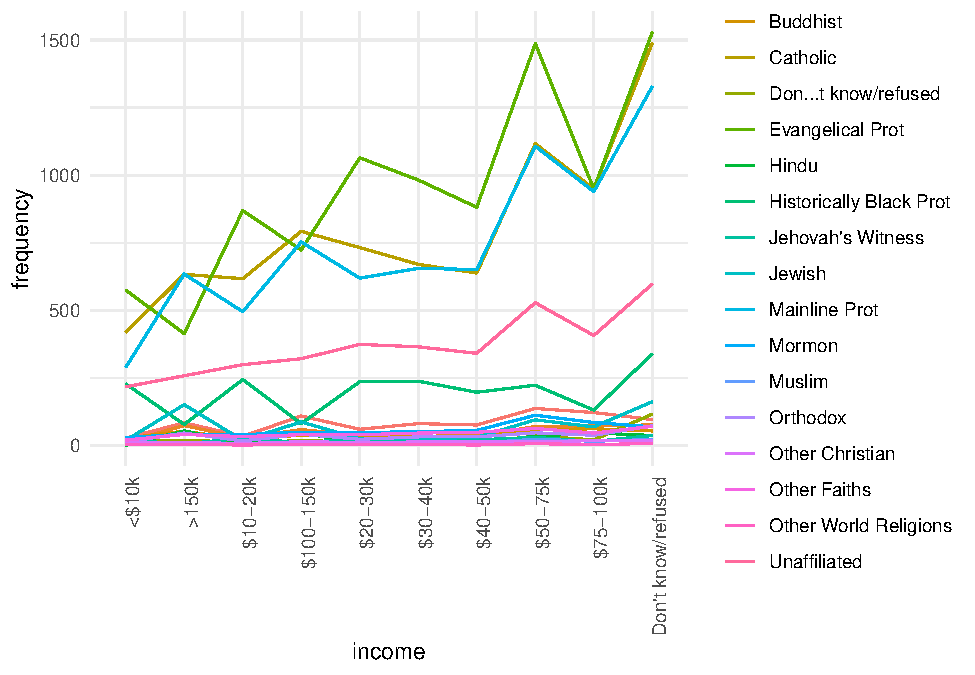
\includegraphics{_main_files/figure-latex/unnamed-chunk-122-1} \end{center}

Podemos hacer gráficas más interesantes si creamos nuevas variables:

\begin{Shaded}
\begin{Highlighting}[]
\NormalTok{by\_religion }\OtherTok{\textless{}{-}} \FunctionTok{group\_by}\NormalTok{(pew\_tidy, religion)}
\NormalTok{pew\_tidy\_2 }\OtherTok{\textless{}{-}}\NormalTok{ pew\_tidy }\SpecialCharTok{\%\textgreater{}\%}
  \FunctionTok{filter}\NormalTok{(income }\SpecialCharTok{!=} \StringTok{"Don\textquotesingle{}t know/refused"}\NormalTok{) }\SpecialCharTok{\%\textgreater{}\%}
  \FunctionTok{group\_by}\NormalTok{(religion) }\SpecialCharTok{\%\textgreater{}\%}
  \FunctionTok{mutate}\NormalTok{(}\AttributeTok{percent =}\NormalTok{ frequency }\SpecialCharTok{/} \FunctionTok{sum}\NormalTok{(frequency)) }\SpecialCharTok{\%\textgreater{}\%} 
  \FunctionTok{filter}\NormalTok{(}\FunctionTok{sum}\NormalTok{(frequency) }\SpecialCharTok{\textgreater{}} \DecValTok{1000}\NormalTok{)}
\FunctionTok{head}\NormalTok{(pew\_tidy\_2)}
\CommentTok{\#\textgreater{} \# A tibble: 6 x 4}
\CommentTok{\#\textgreater{} \# Groups:   religion [5]}
\CommentTok{\#\textgreater{}   religion                income  frequency percent}
\CommentTok{\#\textgreater{}   \textless{}chr\textgreater{}                   \textless{}chr\textgreater{}       \textless{}dbl\textgreater{}   \textless{}dbl\textgreater{}}
\CommentTok{\#\textgreater{} 1 Catholic                \textless{}$10k         418  0.0637}
\CommentTok{\#\textgreater{} 2 Evangelical Prot        \textless{}$10k         575  0.0724}
\CommentTok{\#\textgreater{} 3 Historically Black Prot \textless{}$10k         228  0.138 }
\CommentTok{\#\textgreater{} 4 Mainline Prot           \textless{}$10k         289  0.0471}
\CommentTok{\#\textgreater{} 5 Unaffiliated            \textless{}$10k         217  0.0698}
\CommentTok{\#\textgreater{} 6 Catholic                $10{-}20k       617  0.0940}
\NormalTok{income\_levels }\OtherTok{\textless{}{-}} \FunctionTok{unique}\NormalTok{(pew\_tidy}\SpecialCharTok{$}\NormalTok{income)[}\DecValTok{1}\SpecialCharTok{:}\DecValTok{9}\NormalTok{]}
\FunctionTok{ggplot}\NormalTok{(pew\_tidy\_2, }\FunctionTok{aes}\NormalTok{(}\AttributeTok{x =}\NormalTok{ income, }\AttributeTok{y =}\NormalTok{ percent, }\AttributeTok{group =}\NormalTok{ religion)) }\SpecialCharTok{+}
  \FunctionTok{facet\_wrap}\NormalTok{(}\SpecialCharTok{\textasciitilde{}}\NormalTok{ religion, }\AttributeTok{nrow =} \DecValTok{1}\NormalTok{) }\SpecialCharTok{+}
  \FunctionTok{geom\_bar}\NormalTok{(}\AttributeTok{stat =} \StringTok{"identity"}\NormalTok{, }\AttributeTok{fill =} \StringTok{"darkgray"}\NormalTok{) }\SpecialCharTok{+} 
  \FunctionTok{theme}\NormalTok{(}\AttributeTok{axis.text.x =} \FunctionTok{element\_text}\NormalTok{(}\AttributeTok{angle =} \DecValTok{90}\NormalTok{, }\AttributeTok{hjust =} \DecValTok{1}\NormalTok{)) }\SpecialCharTok{+}
    \FunctionTok{scale\_x\_discrete}\NormalTok{(}\AttributeTok{limits =}\NormalTok{ income\_levels)}
\end{Highlighting}
\end{Shaded}

\begin{center}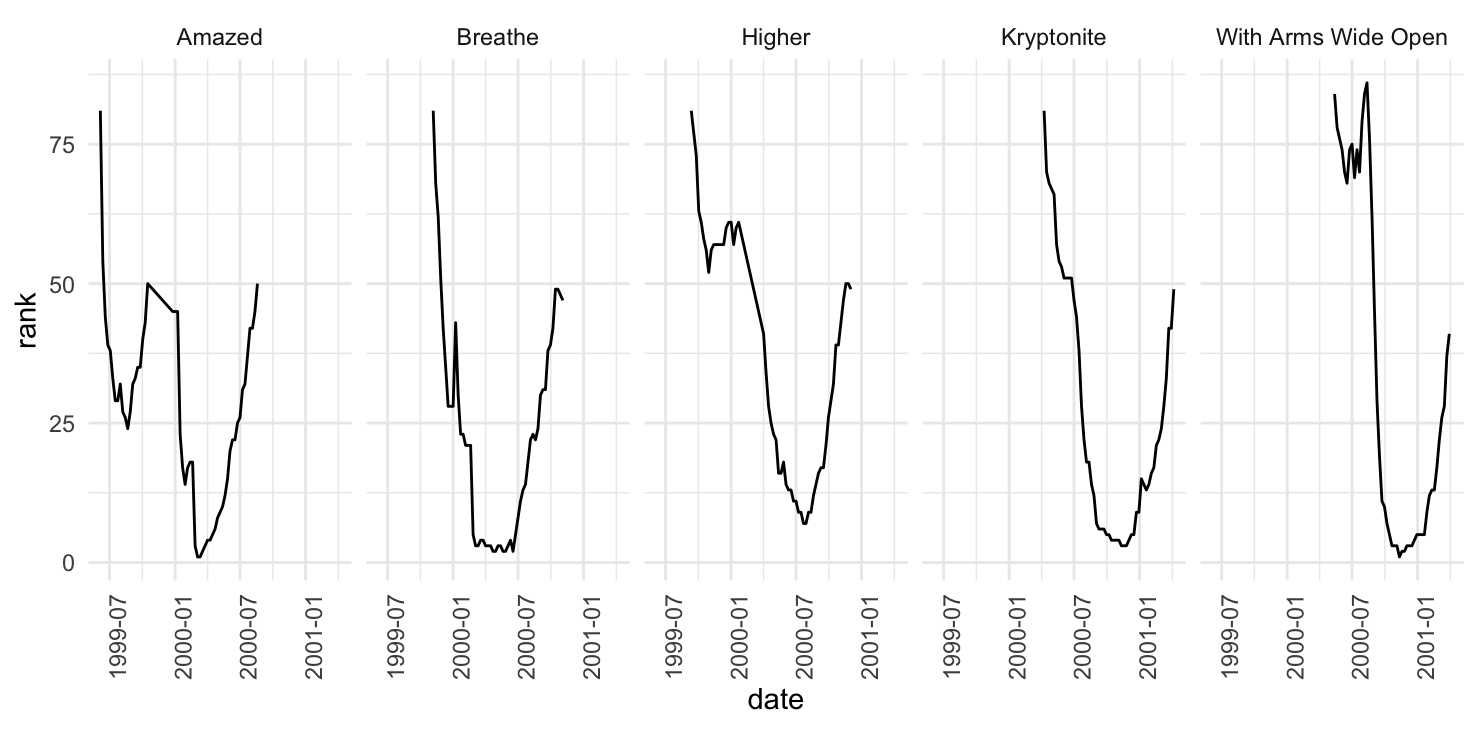
\includegraphics{_main_files/figure-latex/unnamed-chunk-123-1} \end{center}

En el código de arriba utilizamos las funciones \texttt{group\_by}, \texttt{filter} y \texttt{mutate}
que estudiaremos más adelante. Por ahora concentremonos en \texttt{gather} y \texttt{spread}.

Otro ejemplo, veamos los datos de \emph{Billboard}, aquí se registra la fecha en la
que una canción entra por primera vez al top 100 de Billboard.

\begin{Shaded}
\begin{Highlighting}[]
\NormalTok{billboard }\OtherTok{\textless{}{-}} \FunctionTok{read\_csv}\NormalTok{(}\StringTok{"data/billboard.csv"}\NormalTok{)}
\CommentTok{\#\textgreater{} Rows: 317 Columns: 81}
\CommentTok{\#\textgreater{} {-}{-} Column specification {-}{-}{-}{-}{-}{-}{-}{-}{-}{-}{-}{-}{-}{-}{-}{-}{-}{-}{-}{-}{-}{-}{-}{-}{-}{-}{-}{-}{-}{-}{-}{-}{-}{-}{-}{-}{-}{-}{-}{-}{-}{-}{-}{-}{-}{-}{-}{-}{-}{-}{-}{-}{-}{-}{-}{-}}
\CommentTok{\#\textgreater{} Delimiter: ","}
\CommentTok{\#\textgreater{} chr   (2): artist, track}
\CommentTok{\#\textgreater{} dbl  (66): year, wk1, wk2, wk3, wk4, wk5, wk6, wk7, wk8, wk9, wk10, wk11, wk...}
\CommentTok{\#\textgreater{} lgl  (11): wk66, wk67, wk68, wk69, wk70, wk71, wk72, wk73, wk74, wk75, wk76}
\CommentTok{\#\textgreater{} date  (1): date.entered}
\CommentTok{\#\textgreater{} time  (1): time}
\CommentTok{\#\textgreater{} }
\CommentTok{\#\textgreater{} i Use \textasciigrave{}spec()\textasciigrave{} to retrieve the full column specification for this data.}
\CommentTok{\#\textgreater{} i Specify the column types or set \textasciigrave{}show\_col\_types = FALSE\textasciigrave{} to quiet this message.}
\NormalTok{billboard}
\CommentTok{\#\textgreater{} \# A tibble: 317 x 81}
\CommentTok{\#\textgreater{}     year artist track time  date.ent\textasciitilde{}1   wk1   wk2   wk3   wk4   wk5   wk6   wk7}
\CommentTok{\#\textgreater{}    \textless{}dbl\textgreater{} \textless{}chr\textgreater{}  \textless{}chr\textgreater{} \textless{}tim\textgreater{} \textless{}date\textgreater{}     \textless{}dbl\textgreater{} \textless{}dbl\textgreater{} \textless{}dbl\textgreater{} \textless{}dbl\textgreater{} \textless{}dbl\textgreater{} \textless{}dbl\textgreater{} \textless{}dbl\textgreater{}}
\CommentTok{\#\textgreater{}  1  2000 2 Pac  Baby\textasciitilde{} 04:22 2000{-}02{-}26    87    82    72    77    87    94    99}
\CommentTok{\#\textgreater{}  2  2000 2Ge+h\textasciitilde{} The \textasciitilde{} 03:15 2000{-}09{-}02    91    87    92    NA    NA    NA    NA}
\CommentTok{\#\textgreater{}  3  2000 3 Doo\textasciitilde{} Kryp\textasciitilde{} 03:53 2000{-}04{-}08    81    70    68    67    66    57    54}
\CommentTok{\#\textgreater{}  4  2000 3 Doo\textasciitilde{} Loser 04:24 2000{-}10{-}21    76    76    72    69    67    65    55}
\CommentTok{\#\textgreater{}  5  2000 504 B\textasciitilde{} Wobb\textasciitilde{} 03:35 2000{-}04{-}15    57    34    25    17    17    31    36}
\CommentTok{\#\textgreater{}  6  2000 98\^{}0   Give\textasciitilde{} 03:24 2000{-}08{-}19    51    39    34    26    26    19     2}
\CommentTok{\#\textgreater{}  7  2000 A*Tee\textasciitilde{} Danc\textasciitilde{} 03:44 2000{-}07{-}08    97    97    96    95   100    NA    NA}
\CommentTok{\#\textgreater{}  8  2000 Aaliy\textasciitilde{} I Do\textasciitilde{} 04:15 2000{-}01{-}29    84    62    51    41    38    35    35}
\CommentTok{\#\textgreater{}  9  2000 Aaliy\textasciitilde{} Try \textasciitilde{} 04:03 2000{-}03{-}18    59    53    38    28    21    18    16}
\CommentTok{\#\textgreater{} 10  2000 Adams\textasciitilde{} Open\textasciitilde{} 05:30 2000{-}08{-}26    76    76    74    69    68    67    61}
\CommentTok{\#\textgreater{} \# ... with 307 more rows, 69 more variables: wk8 \textless{}dbl\textgreater{}, wk9 \textless{}dbl\textgreater{}, wk10 \textless{}dbl\textgreater{},}
\CommentTok{\#\textgreater{} \#   wk11 \textless{}dbl\textgreater{}, wk12 \textless{}dbl\textgreater{}, wk13 \textless{}dbl\textgreater{}, wk14 \textless{}dbl\textgreater{}, wk15 \textless{}dbl\textgreater{}, wk16 \textless{}dbl\textgreater{},}
\CommentTok{\#\textgreater{} \#   wk17 \textless{}dbl\textgreater{}, wk18 \textless{}dbl\textgreater{}, wk19 \textless{}dbl\textgreater{}, wk20 \textless{}dbl\textgreater{}, wk21 \textless{}dbl\textgreater{}, wk22 \textless{}dbl\textgreater{},}
\CommentTok{\#\textgreater{} \#   wk23 \textless{}dbl\textgreater{}, wk24 \textless{}dbl\textgreater{}, wk25 \textless{}dbl\textgreater{}, wk26 \textless{}dbl\textgreater{}, wk27 \textless{}dbl\textgreater{}, wk28 \textless{}dbl\textgreater{},}
\CommentTok{\#\textgreater{} \#   wk29 \textless{}dbl\textgreater{}, wk30 \textless{}dbl\textgreater{}, wk31 \textless{}dbl\textgreater{}, wk32 \textless{}dbl\textgreater{}, wk33 \textless{}dbl\textgreater{}, wk34 \textless{}dbl\textgreater{},}
\CommentTok{\#\textgreater{} \#   wk35 \textless{}dbl\textgreater{}, wk36 \textless{}dbl\textgreater{}, wk37 \textless{}dbl\textgreater{}, wk38 \textless{}dbl\textgreater{}, wk39 \textless{}dbl\textgreater{}, wk40 \textless{}dbl\textgreater{},}
\CommentTok{\#\textgreater{} \#   wk41 \textless{}dbl\textgreater{}, wk42 \textless{}dbl\textgreater{}, wk43 \textless{}dbl\textgreater{}, wk44 \textless{}dbl\textgreater{}, wk45 \textless{}dbl\textgreater{}, wk46 \textless{}dbl\textgreater{}, ...}
\end{Highlighting}
\end{Shaded}

Notemos que el rank en cada semana (una vez que entró a la lista) está guardado
en 75 columnas \texttt{wk1} a \texttt{wk75}, este tipo de almacenamiento no es \emph{limpio} pero
puede ser útil al momento de ingresar la información.

Para tener datos \emph{limpios} apilamos las semanas de manera que sea una sola
columna (nuevamente alargamos los datos):

\begin{Shaded}
\begin{Highlighting}[]
\NormalTok{billboard\_long }\OtherTok{\textless{}{-}} \FunctionTok{gather}\NormalTok{(billboard, week, rank, wk1}\SpecialCharTok{:}\NormalTok{wk76, }\AttributeTok{na.rm =} \ConstantTok{TRUE}\NormalTok{)}
\NormalTok{billboard\_long}
\CommentTok{\#\textgreater{} \# A tibble: 5,307 x 7}
\CommentTok{\#\textgreater{}     year artist         track                   time   date.entered week   rank}
\CommentTok{\#\textgreater{}    \textless{}dbl\textgreater{} \textless{}chr\textgreater{}          \textless{}chr\textgreater{}                   \textless{}time\textgreater{} \textless{}date\textgreater{}       \textless{}chr\textgreater{} \textless{}dbl\textgreater{}}
\CommentTok{\#\textgreater{}  1  2000 2 Pac          Baby Don\textquotesingle{}t Cry (Keep... 04:22  2000{-}02{-}26   wk1      87}
\CommentTok{\#\textgreater{}  2  2000 2Ge+her        The Hardest Part Of ... 03:15  2000{-}09{-}02   wk1      91}
\CommentTok{\#\textgreater{}  3  2000 3 Doors Down   Kryptonite              03:53  2000{-}04{-}08   wk1      81}
\CommentTok{\#\textgreater{}  4  2000 3 Doors Down   Loser                   04:24  2000{-}10{-}21   wk1      76}
\CommentTok{\#\textgreater{}  5  2000 504 Boyz       Wobble Wobble           03:35  2000{-}04{-}15   wk1      57}
\CommentTok{\#\textgreater{}  6  2000 98\^{}0           Give Me Just One Nig... 03:24  2000{-}08{-}19   wk1      51}
\CommentTok{\#\textgreater{}  7  2000 A*Teens        Dancing Queen           03:44  2000{-}07{-}08   wk1      97}
\CommentTok{\#\textgreater{}  8  2000 Aaliyah        I Don\textquotesingle{}t Wanna           04:15  2000{-}01{-}29   wk1      84}
\CommentTok{\#\textgreater{}  9  2000 Aaliyah        Try Again               04:03  2000{-}03{-}18   wk1      59}
\CommentTok{\#\textgreater{} 10  2000 Adams, Yolanda Open My Heart           05:30  2000{-}08{-}26   wk1      76}
\CommentTok{\#\textgreater{} \# ... with 5,297 more rows}
\end{Highlighting}
\end{Shaded}

Notemos que en esta ocasión especificamos las columnas que vamos a apilar
indicando el nombre de la primera de ellas seguido de \texttt{:} y por último el
nombre de la última variable a apilar. Por otra parte, la instrucción
\texttt{na.rm\ =\ TRUE} se utiliza para eliminar los renglones con valores faltantes en
la columna de value (rank), esto es, eliminamos aquellas observaciones que
tenían NA en la columnas wk\emph{num} de la tabla ancha. Ahora realizamos una
limpieza adicional creando mejores variables de fecha.

\begin{Shaded}
\begin{Highlighting}[]
\NormalTok{billboard\_tidy }\OtherTok{\textless{}{-}}\NormalTok{ billboard\_long }\SpecialCharTok{\%\textgreater{}\%}
  \FunctionTok{mutate}\NormalTok{(}
    \AttributeTok{week =} \FunctionTok{parse\_number}\NormalTok{(week),}
    \AttributeTok{date =}\NormalTok{ date.entered }\SpecialCharTok{+} \DecValTok{7} \SpecialCharTok{*}\NormalTok{ (week }\SpecialCharTok{{-}} \DecValTok{1}\NormalTok{), }
    \AttributeTok{rank =} \FunctionTok{as.numeric}\NormalTok{(rank)}
\NormalTok{    ) }\SpecialCharTok{\%\textgreater{}\%}
    \FunctionTok{select}\NormalTok{(}\SpecialCharTok{{-}}\NormalTok{date.entered)}
\NormalTok{billboard\_tidy}
\CommentTok{\#\textgreater{} \# A tibble: 5,307 x 7}
\CommentTok{\#\textgreater{}     year artist         track                   time    week  rank date      }
\CommentTok{\#\textgreater{}    \textless{}dbl\textgreater{} \textless{}chr\textgreater{}          \textless{}chr\textgreater{}                   \textless{}time\textgreater{} \textless{}dbl\textgreater{} \textless{}dbl\textgreater{} \textless{}date\textgreater{}    }
\CommentTok{\#\textgreater{}  1  2000 2 Pac          Baby Don\textquotesingle{}t Cry (Keep... 04:22      1    87 2000{-}02{-}26}
\CommentTok{\#\textgreater{}  2  2000 2Ge+her        The Hardest Part Of ... 03:15      1    91 2000{-}09{-}02}
\CommentTok{\#\textgreater{}  3  2000 3 Doors Down   Kryptonite              03:53      1    81 2000{-}04{-}08}
\CommentTok{\#\textgreater{}  4  2000 3 Doors Down   Loser                   04:24      1    76 2000{-}10{-}21}
\CommentTok{\#\textgreater{}  5  2000 504 Boyz       Wobble Wobble           03:35      1    57 2000{-}04{-}15}
\CommentTok{\#\textgreater{}  6  2000 98\^{}0           Give Me Just One Nig... 03:24      1    51 2000{-}08{-}19}
\CommentTok{\#\textgreater{}  7  2000 A*Teens        Dancing Queen           03:44      1    97 2000{-}07{-}08}
\CommentTok{\#\textgreater{}  8  2000 Aaliyah        I Don\textquotesingle{}t Wanna           04:15      1    84 2000{-}01{-}29}
\CommentTok{\#\textgreater{}  9  2000 Aaliyah        Try Again               04:03      1    59 2000{-}03{-}18}
\CommentTok{\#\textgreater{} 10  2000 Adams, Yolanda Open My Heart           05:30      1    76 2000{-}08{-}26}
\CommentTok{\#\textgreater{} \# ... with 5,297 more rows}
\end{Highlighting}
\end{Shaded}

Nuevamente, podemos hacer gráficas facilmente.

\begin{Shaded}
\begin{Highlighting}[]
\NormalTok{tracks }\OtherTok{\textless{}{-}} \FunctionTok{filter}\NormalTok{(billboard\_tidy, track }\SpecialCharTok{\%in\%} 
    \FunctionTok{c}\NormalTok{(}\StringTok{"Higher"}\NormalTok{, }\StringTok{"Amazed"}\NormalTok{, }\StringTok{"Kryptonite"}\NormalTok{, }\StringTok{"Breathe"}\NormalTok{, }\StringTok{"With Arms Wide Open"}\NormalTok{))}
\FunctionTok{ggplot}\NormalTok{(tracks, }\FunctionTok{aes}\NormalTok{(}\AttributeTok{x =}\NormalTok{ date, }\AttributeTok{y =}\NormalTok{ rank)) }\SpecialCharTok{+}
  \FunctionTok{geom\_line}\NormalTok{() }\SpecialCharTok{+} 
  \FunctionTok{facet\_wrap}\NormalTok{(}\SpecialCharTok{\textasciitilde{}}\NormalTok{track, }\AttributeTok{nrow =} \DecValTok{1}\NormalTok{) }\SpecialCharTok{+} 
  \FunctionTok{theme}\NormalTok{(}\AttributeTok{axis.text.x =} \FunctionTok{element\_text}\NormalTok{(}\AttributeTok{angle =} \DecValTok{90}\NormalTok{, }\AttributeTok{hjust =} \DecValTok{1}\NormalTok{))}
\end{Highlighting}
\end{Shaded}

\begin{center}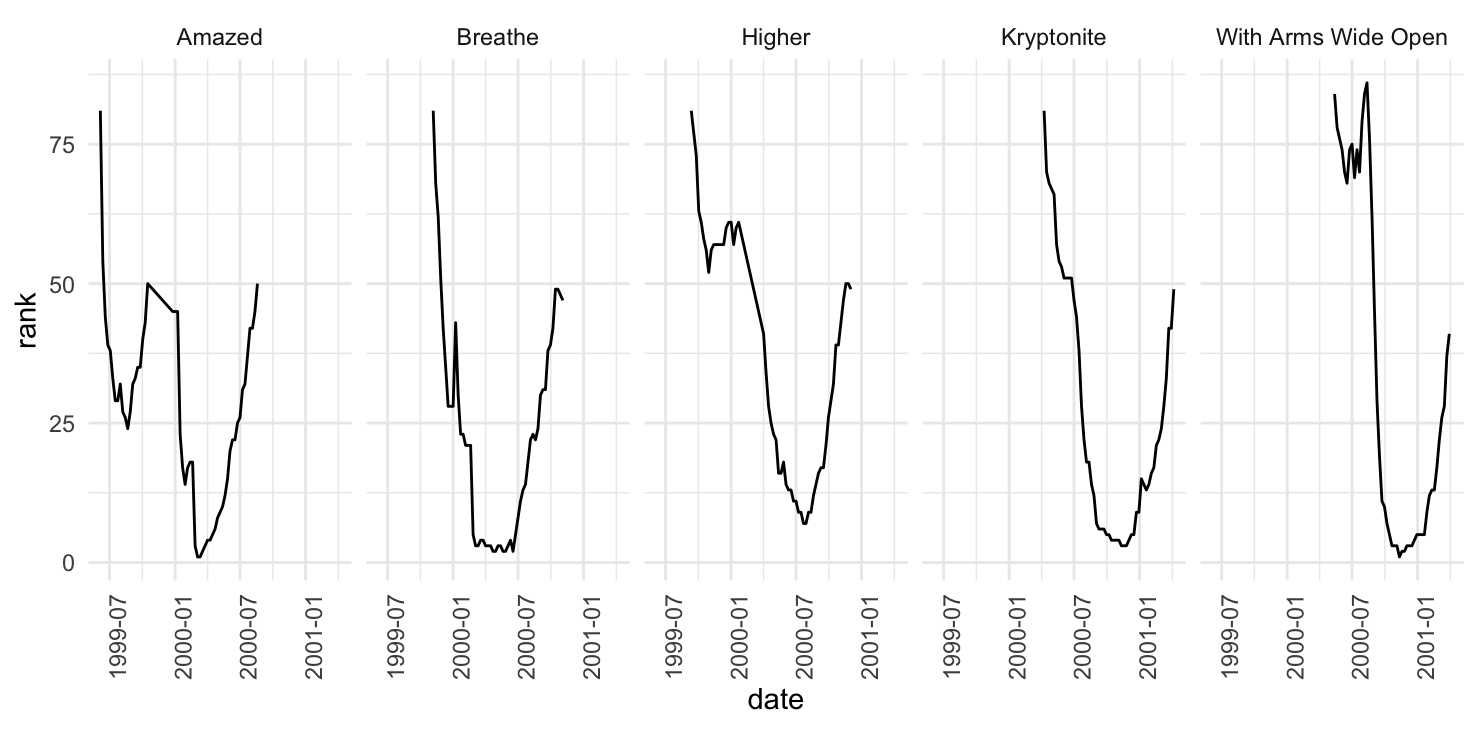
\includegraphics{_main_files/figure-latex/unnamed-chunk-127-1} \end{center}

\hypertarget{una-columna-asociada-a-muxe1s-de-una-variable}{%
\subsection*{Una columna asociada a más de una variable}\label{una-columna-asociada-a-muxe1s-de-una-variable}}
\addcontentsline{toc}{subsection}{Una columna asociada a más de una variable}

La siguiente base de datos proviene de la Organización Mundial de la Salud y
contiene el número de casos confirmados de tuberculosis por país y año, la
información esta por grupo demográfico de acuerdo a sexo (m, f), y edad (0-4,
5-14, etc). Los datos están disponibles en \url{http://www.who.int/tb/country/data/download/en/}.

\begin{Shaded}
\begin{Highlighting}[]
\NormalTok{tb }\OtherTok{\textless{}{-}} \FunctionTok{read.csv}\NormalTok{(}\StringTok{"data/tb.csv"}\NormalTok{) }\SpecialCharTok{\%\textgreater{}\%} \FunctionTok{tbl\_df}\NormalTok{()}
\CommentTok{\#\textgreater{} Warning: \textasciigrave{}tbl\_df()\textasciigrave{} was deprecated in dplyr 1.0.0.}
\CommentTok{\#\textgreater{} i Please use \textasciigrave{}tibble::as\_tibble()\textasciigrave{} instead.}
\NormalTok{tb}
\CommentTok{\#\textgreater{} \# A tibble: 5,769 x 22}
\CommentTok{\#\textgreater{}    iso2   year new\_sp\_\textasciitilde{}1 new\_s\textasciitilde{}2 new\_s\textasciitilde{}3 new\_s\textasciitilde{}4 new\_s\textasciitilde{}5 new\_s\textasciitilde{}6 new\_s\textasciitilde{}7 new\_s\textasciitilde{}8}
\CommentTok{\#\textgreater{}    \textless{}fct\textgreater{} \textless{}int\textgreater{}     \textless{}int\textgreater{}   \textless{}int\textgreater{}   \textless{}int\textgreater{}   \textless{}int\textgreater{}   \textless{}int\textgreater{}   \textless{}int\textgreater{}   \textless{}int\textgreater{}   \textless{}int\textgreater{}}
\CommentTok{\#\textgreater{}  1 AD     1989        NA      NA      NA      NA      NA      NA      NA      NA}
\CommentTok{\#\textgreater{}  2 AD     1990        NA      NA      NA      NA      NA      NA      NA      NA}
\CommentTok{\#\textgreater{}  3 AD     1991        NA      NA      NA      NA      NA      NA      NA      NA}
\CommentTok{\#\textgreater{}  4 AD     1992        NA      NA      NA      NA      NA      NA      NA      NA}
\CommentTok{\#\textgreater{}  5 AD     1993        NA      NA      NA      NA      NA      NA      NA      NA}
\CommentTok{\#\textgreater{}  6 AD     1994        NA      NA      NA      NA      NA      NA      NA      NA}
\CommentTok{\#\textgreater{}  7 AD     1996        NA      NA       0       0       0       4       1       0}
\CommentTok{\#\textgreater{}  8 AD     1997        NA      NA       0       0       1       2       2       1}
\CommentTok{\#\textgreater{}  9 AD     1998        NA      NA       0       0       0       1       0       0}
\CommentTok{\#\textgreater{} 10 AD     1999        NA      NA       0       0       0       1       1       0}
\CommentTok{\#\textgreater{} \# ... with 5,759 more rows, 12 more variables: new\_sp\_m65 \textless{}int\textgreater{},}
\CommentTok{\#\textgreater{} \#   new\_sp\_mu \textless{}int\textgreater{}, new\_sp\_f04 \textless{}int\textgreater{}, new\_sp\_f514 \textless{}int\textgreater{}, new\_sp\_f014 \textless{}int\textgreater{},}
\CommentTok{\#\textgreater{} \#   new\_sp\_f1524 \textless{}int\textgreater{}, new\_sp\_f2534 \textless{}int\textgreater{}, new\_sp\_f3544 \textless{}int\textgreater{},}
\CommentTok{\#\textgreater{} \#   new\_sp\_f4554 \textless{}int\textgreater{}, new\_sp\_f5564 \textless{}int\textgreater{}, new\_sp\_f65 \textless{}int\textgreater{}, new\_sp\_fu \textless{}int\textgreater{},}
\CommentTok{\#\textgreater{} \#   and abbreviated variable names 1: new\_sp\_m04, 2: new\_sp\_m514,}
\CommentTok{\#\textgreater{} \#   3: new\_sp\_m014, 4: new\_sp\_m1524, 5: new\_sp\_m2534, 6: new\_sp\_m3544,}
\CommentTok{\#\textgreater{} \#   7: new\_sp\_m4554, 8: new\_sp\_m5564}
\end{Highlighting}
\end{Shaded}


\includegraphics{imagenes/manicule2.jpg} De manera similar a los ejemplos anteriores,
utiliza la función \texttt{gather} para apilar las columnas correspondientes a
sexo-edad.

~~~~~~~~~~~ Piensa en
como podemos separar la ``variable'' sexo-edad en dos columnas.

Ahora separaremos las variables sexo y edad de la columna demo, para ello
debemos pasar a la función \texttt{separate()}, esta recibe como parámetros:

\begin{itemize}
\item
  el nombre de la base de datos,
\item
  el nombre de la variable que deseamos separar en más de una,
\item
  la posición de donde deseamos ``cortar'' (hay más opciones para especificar
  como separar, ver \texttt{?separate}). El default es separar valores en todos los
  lugares que encuentre un caracter que no es alfanumérico (espacio, guión,\ldots).
\end{itemize}

\begin{Shaded}
\begin{Highlighting}[]
\NormalTok{tb\_tidy }\OtherTok{\textless{}{-}} \FunctionTok{separate}\NormalTok{(tb\_long, demo, }\FunctionTok{c}\NormalTok{(}\StringTok{"sex"}\NormalTok{, }\StringTok{"age"}\NormalTok{), }\DecValTok{8}\NormalTok{)}
\NormalTok{tb\_tidy}
\CommentTok{\#\textgreater{} \# A tibble: 35,750 x 5}
\CommentTok{\#\textgreater{}    iso2   year sex      age       n}
\CommentTok{\#\textgreater{}    \textless{}fct\textgreater{} \textless{}int\textgreater{} \textless{}chr\textgreater{}    \textless{}chr\textgreater{} \textless{}int\textgreater{}}
\CommentTok{\#\textgreater{}  1 AD     2005 new\_sp\_m 04        0}
\CommentTok{\#\textgreater{}  2 AD     2006 new\_sp\_m 04        0}
\CommentTok{\#\textgreater{}  3 AD     2008 new\_sp\_m 04        0}
\CommentTok{\#\textgreater{}  4 AE     2006 new\_sp\_m 04        0}
\CommentTok{\#\textgreater{}  5 AE     2007 new\_sp\_m 04        0}
\CommentTok{\#\textgreater{}  6 AE     2008 new\_sp\_m 04        0}
\CommentTok{\#\textgreater{}  7 AG     2007 new\_sp\_m 04        0}
\CommentTok{\#\textgreater{}  8 AL     2005 new\_sp\_m 04        0}
\CommentTok{\#\textgreater{}  9 AL     2006 new\_sp\_m 04        1}
\CommentTok{\#\textgreater{} 10 AL     2007 new\_sp\_m 04        0}
\CommentTok{\#\textgreater{} \# ... with 35,740 more rows}
\FunctionTok{table}\NormalTok{(tb\_tidy}\SpecialCharTok{$}\NormalTok{sex)}
\CommentTok{\#\textgreater{} }
\CommentTok{\#\textgreater{} new\_sp\_f new\_sp\_m }
\CommentTok{\#\textgreater{}    17830    17920}
\CommentTok{\# creamos un mejor código de genero}
\NormalTok{tb\_tidy }\OtherTok{\textless{}{-}} \FunctionTok{mutate}\NormalTok{(tb\_tidy, }\AttributeTok{sex =} \FunctionTok{substr}\NormalTok{(sex, }\DecValTok{8}\NormalTok{, }\DecValTok{8}\NormalTok{))}
\FunctionTok{table}\NormalTok{(tb\_tidy}\SpecialCharTok{$}\NormalTok{sex)}
\CommentTok{\#\textgreater{} }
\CommentTok{\#\textgreater{}     f     m }
\CommentTok{\#\textgreater{} 17830 17920}
\end{Highlighting}
\end{Shaded}

\hypertarget{variables-almacenadas-en-filas-y-columnas}{%
\subsection*{Variables almacenadas en filas y columnas}\label{variables-almacenadas-en-filas-y-columnas}}
\addcontentsline{toc}{subsection}{Variables almacenadas en filas y columnas}

El problema más difícil es cuando las variables están tanto en filas como en
columnas, veamos una base de datos de clima en Cuernavaca. ¿Cuáles son las
variables en estos datos?

\begin{Shaded}
\begin{Highlighting}[]
\NormalTok{clima }\OtherTok{\textless{}{-}} \FunctionTok{read\_delim}\NormalTok{(}\StringTok{"data/clima.txt"}\NormalTok{, }\StringTok{"}\SpecialCharTok{\textbackslash{}t}\StringTok{"}\NormalTok{, }\AttributeTok{escape\_double =} \ConstantTok{FALSE}\NormalTok{, }
    \AttributeTok{trim\_ws =} \ConstantTok{TRUE}\NormalTok{)}
\CommentTok{\#\textgreater{} Rows: 22 Columns: 35}
\CommentTok{\#\textgreater{} {-}{-} Column specification {-}{-}{-}{-}{-}{-}{-}{-}{-}{-}{-}{-}{-}{-}{-}{-}{-}{-}{-}{-}{-}{-}{-}{-}{-}{-}{-}{-}{-}{-}{-}{-}{-}{-}{-}{-}{-}{-}{-}{-}{-}{-}{-}{-}{-}{-}{-}{-}{-}{-}{-}{-}{-}{-}{-}{-}}
\CommentTok{\#\textgreater{} Delimiter: "\textbackslash{}t"}
\CommentTok{\#\textgreater{} chr  (2): id, element}
\CommentTok{\#\textgreater{} dbl (25): year, month, d1, d2, d3, d4, d5, d6, d7, d8, d10, d11, d13, d14, d...}
\CommentTok{\#\textgreater{} lgl  (8): d9, d12, d18, d19, d20, d21, d22, d24}
\CommentTok{\#\textgreater{} }
\CommentTok{\#\textgreater{} i Use \textasciigrave{}spec()\textasciigrave{} to retrieve the full column specification for this data.}
\CommentTok{\#\textgreater{} i Specify the column types or set \textasciigrave{}show\_col\_types = FALSE\textasciigrave{} to quiet this message.}
\end{Highlighting}
\end{Shaded}

Estos datos tienen variables en columnas individuales (id, año, mes), en
múltiples columnas (día, d1-d31) y en filas (tmin, tmax). Comencemos por apilar
las columnas.

\begin{Shaded}
\begin{Highlighting}[]
\NormalTok{clima\_long }\OtherTok{\textless{}{-}} \FunctionTok{gather}\NormalTok{(clima, day, value, d1}\SpecialCharTok{:}\NormalTok{d31, }\AttributeTok{na.rm =} \ConstantTok{TRUE}\NormalTok{)}
\NormalTok{clima\_long}
\CommentTok{\#\textgreater{} \# A tibble: 66 x 6}
\CommentTok{\#\textgreater{}    id           year month element day   value}
\CommentTok{\#\textgreater{}    \textless{}chr\textgreater{}       \textless{}dbl\textgreater{} \textless{}dbl\textgreater{} \textless{}chr\textgreater{}   \textless{}chr\textgreater{} \textless{}dbl\textgreater{}}
\CommentTok{\#\textgreater{}  1 MX000017004  2010    12 TMAX    d1      299}
\CommentTok{\#\textgreater{}  2 MX000017004  2010    12 TMIN    d1      138}
\CommentTok{\#\textgreater{}  3 MX000017004  2010     2 TMAX    d2      273}
\CommentTok{\#\textgreater{}  4 MX000017004  2010     2 TMIN    d2      144}
\CommentTok{\#\textgreater{}  5 MX000017004  2010    11 TMAX    d2      313}
\CommentTok{\#\textgreater{}  6 MX000017004  2010    11 TMIN    d2      163}
\CommentTok{\#\textgreater{}  7 MX000017004  2010     2 TMAX    d3      241}
\CommentTok{\#\textgreater{}  8 MX000017004  2010     2 TMIN    d3      144}
\CommentTok{\#\textgreater{}  9 MX000017004  2010     7 TMAX    d3      286}
\CommentTok{\#\textgreater{} 10 MX000017004  2010     7 TMIN    d3      175}
\CommentTok{\#\textgreater{} \# ... with 56 more rows}
\end{Highlighting}
\end{Shaded}

Podemos crear algunas variables adicionales.

\begin{Shaded}
\begin{Highlighting}[]
\NormalTok{clima\_vars }\OtherTok{\textless{}{-}}\NormalTok{ clima\_long }\SpecialCharTok{\%\textgreater{}\%} 
  \FunctionTok{mutate}\NormalTok{(}\AttributeTok{day =} \FunctionTok{parse\_number}\NormalTok{(day), }
    \AttributeTok{value =} \FunctionTok{as.numeric}\NormalTok{(value) }\SpecialCharTok{/} \DecValTok{10}\NormalTok{) }\SpecialCharTok{\%\textgreater{}\%}
  \FunctionTok{select}\NormalTok{(id, year, month, day, element, value) }\SpecialCharTok{\%\textgreater{}\%}
  \FunctionTok{arrange}\NormalTok{(id, year, month, day)}
\NormalTok{clima\_vars}
\CommentTok{\#\textgreater{} \# A tibble: 66 x 6}
\CommentTok{\#\textgreater{}    id           year month   day element value}
\CommentTok{\#\textgreater{}    \textless{}chr\textgreater{}       \textless{}dbl\textgreater{} \textless{}dbl\textgreater{} \textless{}dbl\textgreater{} \textless{}chr\textgreater{}   \textless{}dbl\textgreater{}}
\CommentTok{\#\textgreater{}  1 MX000017004  2010     1    30 TMAX     27.8}
\CommentTok{\#\textgreater{}  2 MX000017004  2010     1    30 TMIN     14.5}
\CommentTok{\#\textgreater{}  3 MX000017004  2010     2     2 TMAX     27.3}
\CommentTok{\#\textgreater{}  4 MX000017004  2010     2     2 TMIN     14.4}
\CommentTok{\#\textgreater{}  5 MX000017004  2010     2     3 TMAX     24.1}
\CommentTok{\#\textgreater{}  6 MX000017004  2010     2     3 TMIN     14.4}
\CommentTok{\#\textgreater{}  7 MX000017004  2010     2    11 TMAX     29.7}
\CommentTok{\#\textgreater{}  8 MX000017004  2010     2    11 TMIN     13.4}
\CommentTok{\#\textgreater{}  9 MX000017004  2010     2    23 TMAX     29.9}
\CommentTok{\#\textgreater{} 10 MX000017004  2010     2    23 TMIN     10.7}
\CommentTok{\#\textgreater{} \# ... with 56 more rows}
\end{Highlighting}
\end{Shaded}

Finalmente, la columna \emph{element} no es una variable, sino que almacena el nombre
de dos variables, la operación que debemos aplicar (spread) es el inverso de
apilar (\texttt{gather}):

\begin{Shaded}
\begin{Highlighting}[]
\NormalTok{clima\_tidy }\OtherTok{\textless{}{-}} \FunctionTok{spread}\NormalTok{(clima\_vars, element, value)}
\NormalTok{clima\_tidy}
\CommentTok{\#\textgreater{} \# A tibble: 33 x 6}
\CommentTok{\#\textgreater{}    id           year month   day  TMAX  TMIN}
\CommentTok{\#\textgreater{}    \textless{}chr\textgreater{}       \textless{}dbl\textgreater{} \textless{}dbl\textgreater{} \textless{}dbl\textgreater{} \textless{}dbl\textgreater{} \textless{}dbl\textgreater{}}
\CommentTok{\#\textgreater{}  1 MX000017004  2010     1    30  27.8  14.5}
\CommentTok{\#\textgreater{}  2 MX000017004  2010     2     2  27.3  14.4}
\CommentTok{\#\textgreater{}  3 MX000017004  2010     2     3  24.1  14.4}
\CommentTok{\#\textgreater{}  4 MX000017004  2010     2    11  29.7  13.4}
\CommentTok{\#\textgreater{}  5 MX000017004  2010     2    23  29.9  10.7}
\CommentTok{\#\textgreater{}  6 MX000017004  2010     3     5  32.1  14.2}
\CommentTok{\#\textgreater{}  7 MX000017004  2010     3    10  34.5  16.8}
\CommentTok{\#\textgreater{}  8 MX000017004  2010     3    16  31.1  17.6}
\CommentTok{\#\textgreater{}  9 MX000017004  2010     4    27  36.3  16.7}
\CommentTok{\#\textgreater{} 10 MX000017004  2010     5    27  33.2  18.2}
\CommentTok{\#\textgreater{} \# ... with 23 more rows}
\end{Highlighting}
\end{Shaded}

Ahora es inmediato no solo hacer gráficas sino también ajustar un modelo.

\begin{Shaded}
\begin{Highlighting}[]
\CommentTok{\# ajustamos un modelo lineal donde la variable respuesta es temperatura }
\CommentTok{\# máxima, y la variable explicativa es el mes}
\NormalTok{clima\_lm }\OtherTok{\textless{}{-}} \FunctionTok{lm}\NormalTok{(TMAX }\SpecialCharTok{\textasciitilde{}} \FunctionTok{factor}\NormalTok{(month), }\AttributeTok{data =}\NormalTok{ clima\_tidy)}
\FunctionTok{summary}\NormalTok{(clima\_lm)}
\CommentTok{\#\textgreater{} }
\CommentTok{\#\textgreater{} Call:}
\CommentTok{\#\textgreater{} lm(formula = TMAX \textasciitilde{} factor(month), data = clima\_tidy)}
\CommentTok{\#\textgreater{} }
\CommentTok{\#\textgreater{} Residuals:}
\CommentTok{\#\textgreater{}    Min     1Q Median     3Q    Max }
\CommentTok{\#\textgreater{}  {-}3.65  {-}0.92  {-}0.02   1.05   3.18 }
\CommentTok{\#\textgreater{} }
\CommentTok{\#\textgreater{} Coefficients:}
\CommentTok{\#\textgreater{}                 Estimate Std. Error t value Pr(\textgreater{}|t|)    }
\CommentTok{\#\textgreater{} (Intercept)      27.8000     1.8610  14.938 5.34e{-}13 ***}
\CommentTok{\#\textgreater{} factor(month)2   {-}0.0500     2.0807  {-}0.024  0.98104    }
\CommentTok{\#\textgreater{} factor(month)3    4.7667     2.1489   2.218  0.03717 *  }
\CommentTok{\#\textgreater{} factor(month)4    8.5000     2.6319   3.230  0.00385 ** }
\CommentTok{\#\textgreater{} factor(month)5    5.4000     2.6319   2.052  0.05228 .  }
\CommentTok{\#\textgreater{} factor(month)6    1.2500     2.2793   0.548  0.58892    }
\CommentTok{\#\textgreater{} factor(month)7    1.4500     2.2793   0.636  0.53123    }
\CommentTok{\#\textgreater{} factor(month)8    0.4714     1.9895   0.237  0.81488    }
\CommentTok{\#\textgreater{} factor(month)10   1.1000     2.0386   0.540  0.59491    }
\CommentTok{\#\textgreater{} factor(month)11   0.3200     2.0386   0.157  0.87670    }
\CommentTok{\#\textgreater{} factor(month)12   1.0500     2.2793   0.461  0.64955    }
\CommentTok{\#\textgreater{} {-}{-}{-}}
\CommentTok{\#\textgreater{} Signif. codes:  0 \textquotesingle{}***\textquotesingle{} 0.001 \textquotesingle{}**\textquotesingle{} 0.01 \textquotesingle{}*\textquotesingle{} 0.05 \textquotesingle{}.\textquotesingle{} 0.1 \textquotesingle{} \textquotesingle{} 1}
\CommentTok{\#\textgreater{} }
\CommentTok{\#\textgreater{} Residual standard error: 1.861 on 22 degrees of freedom}
\CommentTok{\#\textgreater{} Multiple R{-}squared:  0.6182, Adjusted R{-}squared:  0.4447 }
\CommentTok{\#\textgreater{} F{-}statistic: 3.563 on 10 and 22 DF,  p{-}value: 0.006196}
\end{Highlighting}
\end{Shaded}

\hypertarget{mas-de-un-tipo-de-observaciuxf3n-en-una-misma-tabla}{%
\subsection*{Mas de un tipo de observación en una misma tabla}\label{mas-de-un-tipo-de-observaciuxf3n-en-una-misma-tabla}}
\addcontentsline{toc}{subsection}{Mas de un tipo de observación en una misma tabla}

En ocasiones las bases de datos involucran valores en diferentes niveles, en
diferentes tipos de unidad observacional. En la limpieza de datos, cada unidad
observacional debe estar almacenada en su propia tabla (esto esta ligado a
normalización de una base de datos), es importante para evitar inconsistencias
en los datos.

¿Cuáles son las unidades observacionales de los datos de billboard?

\begin{Shaded}
\begin{Highlighting}[]
\NormalTok{billboard\_tidy}
\CommentTok{\#\textgreater{} \# A tibble: 5,307 x 7}
\CommentTok{\#\textgreater{}     year artist         track                   time    week  rank date      }
\CommentTok{\#\textgreater{}    \textless{}dbl\textgreater{} \textless{}chr\textgreater{}          \textless{}chr\textgreater{}                   \textless{}time\textgreater{} \textless{}dbl\textgreater{} \textless{}dbl\textgreater{} \textless{}date\textgreater{}    }
\CommentTok{\#\textgreater{}  1  2000 2 Pac          Baby Don\textquotesingle{}t Cry (Keep... 04:22      1    87 2000{-}02{-}26}
\CommentTok{\#\textgreater{}  2  2000 2Ge+her        The Hardest Part Of ... 03:15      1    91 2000{-}09{-}02}
\CommentTok{\#\textgreater{}  3  2000 3 Doors Down   Kryptonite              03:53      1    81 2000{-}04{-}08}
\CommentTok{\#\textgreater{}  4  2000 3 Doors Down   Loser                   04:24      1    76 2000{-}10{-}21}
\CommentTok{\#\textgreater{}  5  2000 504 Boyz       Wobble Wobble           03:35      1    57 2000{-}04{-}15}
\CommentTok{\#\textgreater{}  6  2000 98\^{}0           Give Me Just One Nig... 03:24      1    51 2000{-}08{-}19}
\CommentTok{\#\textgreater{}  7  2000 A*Teens        Dancing Queen           03:44      1    97 2000{-}07{-}08}
\CommentTok{\#\textgreater{}  8  2000 Aaliyah        I Don\textquotesingle{}t Wanna           04:15      1    84 2000{-}01{-}29}
\CommentTok{\#\textgreater{}  9  2000 Aaliyah        Try Again               04:03      1    59 2000{-}03{-}18}
\CommentTok{\#\textgreater{} 10  2000 Adams, Yolanda Open My Heart           05:30      1    76 2000{-}08{-}26}
\CommentTok{\#\textgreater{} \# ... with 5,297 more rows}
\end{Highlighting}
\end{Shaded}

Separemos esta base de datos en dos: la tabla canción que almacena artista,
nombre de la canción y duración; la tabla rank que almacena el ranking de la
canción en cada semana.

\begin{Shaded}
\begin{Highlighting}[]
\NormalTok{song }\OtherTok{\textless{}{-}}\NormalTok{ billboard\_tidy }\SpecialCharTok{\%\textgreater{}\%} 
  \FunctionTok{select}\NormalTok{(artist, track, year, time) }\SpecialCharTok{\%\textgreater{}\%}
  \FunctionTok{unique}\NormalTok{() }\SpecialCharTok{\%\textgreater{}\%}
  \FunctionTok{arrange}\NormalTok{(artist) }\SpecialCharTok{\%\textgreater{}\%}
  \FunctionTok{mutate}\NormalTok{(}\AttributeTok{song\_id =} \FunctionTok{row\_number}\NormalTok{(artist))}
\NormalTok{song}
\CommentTok{\#\textgreater{} \# A tibble: 317 x 5}
\CommentTok{\#\textgreater{}    artist         track                    year time   song\_id}
\CommentTok{\#\textgreater{}    \textless{}chr\textgreater{}          \textless{}chr\textgreater{}                   \textless{}dbl\textgreater{} \textless{}time\textgreater{}   \textless{}int\textgreater{}}
\CommentTok{\#\textgreater{}  1 2 Pac          Baby Don\textquotesingle{}t Cry (Keep...  2000 04:22        1}
\CommentTok{\#\textgreater{}  2 2Ge+her        The Hardest Part Of ...  2000 03:15        2}
\CommentTok{\#\textgreater{}  3 3 Doors Down   Kryptonite               2000 03:53        3}
\CommentTok{\#\textgreater{}  4 3 Doors Down   Loser                    2000 04:24        4}
\CommentTok{\#\textgreater{}  5 504 Boyz       Wobble Wobble            2000 03:35        5}
\CommentTok{\#\textgreater{}  6 98\^{}0           Give Me Just One Nig...  2000 03:24        6}
\CommentTok{\#\textgreater{}  7 A*Teens        Dancing Queen            2000 03:44        7}
\CommentTok{\#\textgreater{}  8 Aaliyah        I Don\textquotesingle{}t Wanna            2000 04:15        8}
\CommentTok{\#\textgreater{}  9 Aaliyah        Try Again                2000 04:03        9}
\CommentTok{\#\textgreater{} 10 Adams, Yolanda Open My Heart            2000 05:30       10}
\CommentTok{\#\textgreater{} \# ... with 307 more rows}
\NormalTok{rank }\OtherTok{\textless{}{-}}\NormalTok{ billboard\_tidy }\SpecialCharTok{\%\textgreater{}\%}
  \FunctionTok{left\_join}\NormalTok{(song, }\FunctionTok{c}\NormalTok{(}\StringTok{"artist"}\NormalTok{, }\StringTok{"track"}\NormalTok{, }\StringTok{"year"}\NormalTok{, }\StringTok{"time"}\NormalTok{)) }\SpecialCharTok{\%\textgreater{}\%}
  \FunctionTok{select}\NormalTok{(song\_id, date, week, rank) }\SpecialCharTok{\%\textgreater{}\%}
  \FunctionTok{arrange}\NormalTok{(song\_id, date) }\SpecialCharTok{\%\textgreater{}\%}
\NormalTok{  tbl\_df}
\NormalTok{rank}
\CommentTok{\#\textgreater{} \# A tibble: 5,307 x 4}
\CommentTok{\#\textgreater{}    song\_id date        week  rank}
\CommentTok{\#\textgreater{}      \textless{}int\textgreater{} \textless{}date\textgreater{}     \textless{}dbl\textgreater{} \textless{}dbl\textgreater{}}
\CommentTok{\#\textgreater{}  1       1 2000{-}02{-}26     1    87}
\CommentTok{\#\textgreater{}  2       1 2000{-}03{-}04     2    82}
\CommentTok{\#\textgreater{}  3       1 2000{-}03{-}11     3    72}
\CommentTok{\#\textgreater{}  4       1 2000{-}03{-}18     4    77}
\CommentTok{\#\textgreater{}  5       1 2000{-}03{-}25     5    87}
\CommentTok{\#\textgreater{}  6       1 2000{-}04{-}01     6    94}
\CommentTok{\#\textgreater{}  7       1 2000{-}04{-}08     7    99}
\CommentTok{\#\textgreater{}  8       2 2000{-}09{-}02     1    91}
\CommentTok{\#\textgreater{}  9       2 2000{-}09{-}09     2    87}
\CommentTok{\#\textgreater{} 10       2 2000{-}09{-}16     3    92}
\CommentTok{\#\textgreater{} \# ... with 5,297 more rows}
\end{Highlighting}
\end{Shaded}

\hypertarget{una-misma-unidad-observacional-estuxe1-almacenada-en-muxfaltiples-tablas}{%
\subsection*{Una misma unidad observacional está almacenada en múltiples tablas}\label{una-misma-unidad-observacional-estuxe1-almacenada-en-muxfaltiples-tablas}}
\addcontentsline{toc}{subsection}{Una misma unidad observacional está almacenada en múltiples tablas}

También es común que los valores sobre una misma unidad observacional estén
separados en muchas tablas o archivos, es común que estas tablas esten divididas
de acuerdo a una variable, de tal manera que cada archivo representa a una
persona, año o ubicación. Para juntar los archivos hacemos lo siguiente:

\begin{enumerate}
\def\labelenumi{\arabic{enumi}.}
\tightlist
\item
  Leemos los archivos en una lista de tablas.
\item
  Para cada tabla agregamos una columna que registra el nombre del archivo
  original.
\item
  Combinamos las tablas en un solo data frame.
\end{enumerate}

Veamos un ejemplo, descarga la carpeta
\href{https://www.dropbox.com/sh/c0mgho95gwjc1mv/AACVLPr33O6ENW68xmL7hyUna?dl=0}{specdata},
ésta contiene 332 archivos csv que almacenan información de monitoreo de
contaminación en 332 ubicaciones de EUA. Cada archivo contiene información de
una unidad de monitoreo y el número de identificación del monitor es el nombre
del archivo.

Los pasos en R (usando el paquete \texttt{purrr}), primero creamos un vector con los
nombres de los archivos en un directorio, eligiendo aquellos que contengan las
letras ``.csv''.

\begin{Shaded}
\begin{Highlighting}[]
\NormalTok{paths }\OtherTok{\textless{}{-}} \FunctionTok{dir}\NormalTok{(}\StringTok{"data/specdata"}\NormalTok{, }\AttributeTok{pattern =} \StringTok{"}\SpecialCharTok{\textbackslash{}\textbackslash{}}\StringTok{.csv$"}\NormalTok{, }\AttributeTok{full.names =} \ConstantTok{TRUE}\NormalTok{) }
\end{Highlighting}
\end{Shaded}

Después le asignamos el nombre del csv al nombre de cada elemento del vector.
Este paso se realiza para preservar los nombres de los archivos ya que estos
los asignaremos a una variable mas adelante.

\begin{Shaded}
\begin{Highlighting}[]
\NormalTok{paths }\OtherTok{\textless{}{-}} \FunctionTok{set\_names}\NormalTok{(paths, }\FunctionTok{basename}\NormalTok{(paths))}
\end{Highlighting}
\end{Shaded}

La función \texttt{map\_df} itera sobre cada dirección, lee el csv en dicha dirección y
los combina en un data frame.

\begin{Shaded}
\begin{Highlighting}[]
\NormalTok{specdata\_us }\OtherTok{\textless{}{-}} \FunctionTok{map\_df}\NormalTok{(paths, }\SpecialCharTok{\textasciitilde{}}\FunctionTok{read\_csv}\NormalTok{(., }\AttributeTok{col\_types =} \StringTok{"Tddi"}\NormalTok{), }\AttributeTok{.id =} \StringTok{"filename"}\NormalTok{)}
\CommentTok{\# eliminamos la basura del id}
\NormalTok{specdata }\OtherTok{\textless{}{-}}\NormalTok{ specdata\_us }\SpecialCharTok{\%\textgreater{}\%}
  \FunctionTok{mutate}\NormalTok{(}\AttributeTok{monitor =} \FunctionTok{parse\_number}\NormalTok{(filename)) }\SpecialCharTok{\%\textgreater{}\%}
  \FunctionTok{select}\NormalTok{(}\AttributeTok{id =}\NormalTok{ ID, monitor, }\AttributeTok{date =}\NormalTok{ Date, sulfate, nitrate)}
\CommentTok{\#\textgreater{} Error in \textasciigrave{}mutate()\textasciigrave{}:}
\CommentTok{\#\textgreater{} ! Problem while computing \textasciigrave{}monitor = parse\_number(filename)\textasciigrave{}.}
\CommentTok{\#\textgreater{} Caused by error in \textasciigrave{}stopifnot()\textasciigrave{}:}
\CommentTok{\#\textgreater{} ! object \textquotesingle{}filename\textquotesingle{} not found}
\NormalTok{specdata}
\CommentTok{\#\textgreater{} Error in eval(expr, envir, enclos): object \textquotesingle{}specdata\textquotesingle{} not found}
\end{Highlighting}
\end{Shaded}

\hypertarget{otras-consideraciones}{%
\subsection*{Otras consideraciones}\label{otras-consideraciones}}
\addcontentsline{toc}{subsection}{Otras consideraciones}

En las buenas prácticas es importante tomar en cuenta los siguientes puntos:

\begin{itemize}
\item
  Incluir un encabezado con el nombre de las variables.
\item
  Los nombres de las variables deben ser entendibles (e.g.~AgeAtDiagnosis es
  mejor que AgeDx).
\item
  En general los datos se deben guardar en un archivo por tabla.
\item
  Escribir un script con las modificaciones que se hicieron a los \emph{datos crudos}
  (reproducibilidad).
\item
  Otros aspectos importantes en la \emph{limpieza} de datos son: selección del tipo
  de variables (por ejemplo fechas), datos faltantes, \emph{typos} y detección de
  valores atípicos.
\end{itemize}

\hypertarget{recursos-adicionales}{%
\subsection*{Recursos adicionales}\label{recursos-adicionales}}
\addcontentsline{toc}{subsection}{Recursos adicionales}

\begin{itemize}
\item
  \href{https://github.com/rstudio/cheatsheets/raw/master/data-import.pdf}{Data Import Cheat Sheet},
  RStudio.
\item
  \href{https://github.com/rstudio/cheatsheets/raw/master/data-transformation.pdf}{Data Transformation Cheat Sheet},
  RStudio.
\end{itemize}

\hypertarget{tarea}{%
\chapter{Tarea}\label{tarea}}

\hypertarget{tarea-1-estructuras-de-datos}{%
\section{Tarea 1: Estructuras de Datos}\label{tarea-1-estructuras-de-datos}}

\begin{itemize}
\tightlist
\item
  Crea un Script nuevo y llámalo ``Tarea\_tunombre.R''.
\item
  Descarga el archivo ``crimen\_mexico.csv'' dándo clic en esta \href{https://www.dropbox.com/s/nq3sg9gnvis3ezy/crimen_mexico.csv?dl=1}{liga} .\\
\item
  Carga la librería \textbf{readr}.
\item
  Utiliza la función \textbf{read\_csv} para cargar el archivo ``crimen\_mexico.csv''. Ojo: recuerda asignarlo a una variable \textbf{datos \textless- read\_csv(``path al archivo'')}.
\item
  Utiliza la función \textbf{summary()} para ver qué variables tienen NA.
\item
  Usa lo visto en clase para quitar las filas con variables faltantes.
\item
  Contesta las siguientes preguntas:
\item
  ¿De qué años hay información?
\item
  ¿Cuál fue el total de crimenes en 2022 y 2021?
\item
  Haz un subset de datos considerando solamente los datos de 2022.
\item
  ¿Cuál fue el total de delitos por estado?
\item
  ¿Cuál fue el promedio de delitos por mes?
\item
  ¿Cuál fue el tipo de delitos con mayor y menor incidencia?
\end{itemize}

\hypertarget{respuesta-tarea-1-estructuras-de-datos}{%
\section{Respuesta Tarea 1: Estructuras de Datos}\label{respuesta-tarea-1-estructuras-de-datos}}

Carga la librería \textbf{readr}

\begin{Shaded}
\begin{Highlighting}[]
\FunctionTok{library}\NormalTok{(readr)}
\end{Highlighting}
\end{Shaded}

\begin{itemize}
\tightlist
\item
  Utiliza la función \textbf{read\_csv} para cargar el archivo ``crimen\_mexico.csv''. Ojo: recuerda asignarlo a una variable \textbf{datos \textless- read\_csv(``path al archivo'')}.
\end{itemize}

\begin{Shaded}
\begin{Highlighting}[]
\NormalTok{datos }\OtherTok{\textless{}{-}} \FunctionTok{read\_csv}\NormalTok{(}\StringTok{"data/crimen\_mexico.csv"}\NormalTok{)}
\CommentTok{\#\textgreater{} Rows: 75264 Columns: 6}
\CommentTok{\#\textgreater{} {-}{-} Column specification {-}{-}{-}{-}{-}{-}{-}{-}{-}{-}{-}{-}{-}{-}{-}{-}{-}{-}{-}{-}{-}{-}{-}{-}{-}{-}{-}{-}{-}{-}{-}{-}{-}{-}{-}{-}{-}{-}{-}{-}{-}{-}{-}{-}{-}{-}{-}{-}{-}{-}{-}{-}{-}{-}{-}{-}}
\CommentTok{\#\textgreater{} Delimiter: ","}
\CommentTok{\#\textgreater{} chr  (3): entidad, tipo\_delito, mes}
\CommentTok{\#\textgreater{} dbl  (2): año, total\_Delitos}
\CommentTok{\#\textgreater{} date (1): fecha}
\CommentTok{\#\textgreater{} }
\CommentTok{\#\textgreater{} i Use \textasciigrave{}spec()\textasciigrave{} to retrieve the full column specification for this data.}
\CommentTok{\#\textgreater{} i Specify the column types or set \textasciigrave{}show\_col\_types = FALSE\textasciigrave{} to quiet this message.}
\FunctionTok{head}\NormalTok{(datos)}
\CommentTok{\#\textgreater{} \# A tibble: 6 x 6}
\CommentTok{\#\textgreater{}     año entidad        tipo\_delito mes     fecha      total\_Delitos}
\CommentTok{\#\textgreater{}   \textless{}dbl\textgreater{} \textless{}chr\textgreater{}          \textless{}chr\textgreater{}       \textless{}chr\textgreater{}   \textless{}date\textgreater{}             \textless{}dbl\textgreater{}}
\CommentTok{\#\textgreater{} 1  2021 Aguascalientes Homicidio   Enero   2021{-}01{-}01             2}
\CommentTok{\#\textgreater{} 2  2021 Aguascalientes Homicidio   Febrero 2021{-}02{-}01             1}
\CommentTok{\#\textgreater{} 3  2021 Aguascalientes Homicidio   Marzo   2021{-}03{-}01             4}
\CommentTok{\#\textgreater{} 4  2021 Aguascalientes Homicidio   Abril   2021{-}04{-}01             3}
\CommentTok{\#\textgreater{} 5  2021 Aguascalientes Homicidio   Mayo    2021{-}05{-}01             4}
\CommentTok{\#\textgreater{} 6  2021 Aguascalientes Homicidio   Junio   2021{-}06{-}01             2}
\end{Highlighting}
\end{Shaded}

\begin{itemize}
\tightlist
\item
  Utiliza la función \textbf{summary()} para ver qué variables tienen NA.
\end{itemize}

\begin{Shaded}
\begin{Highlighting}[]
\FunctionTok{summary}\NormalTok{(datos)}
\CommentTok{\#\textgreater{}       año         entidad          tipo\_delito            mes           }
\CommentTok{\#\textgreater{}  Min.   :2021   Length:75264       Length:75264       Length:75264      }
\CommentTok{\#\textgreater{}  1st Qu.:2021   Class :character   Class :character   Class :character  }
\CommentTok{\#\textgreater{}  Median :2022   Mode  :character   Mode  :character   Mode  :character  }
\CommentTok{\#\textgreater{}  Mean   :2022                                                           }
\CommentTok{\#\textgreater{}  3rd Qu.:2022                                                           }
\CommentTok{\#\textgreater{}  Max.   :2022                                                           }
\CommentTok{\#\textgreater{}                                                                         }
\CommentTok{\#\textgreater{}      fecha            total\_Delitos    }
\CommentTok{\#\textgreater{}  Min.   :2021{-}01{-}01   Min.   :   0.00  }
\CommentTok{\#\textgreater{}  1st Qu.:2021{-}06{-}23   1st Qu.:   0.00  }
\CommentTok{\#\textgreater{}  Median :2021{-}12{-}16   Median :   2.00  }
\CommentTok{\#\textgreater{}  Mean   :2021{-}12{-}16   Mean   :  55.53  }
\CommentTok{\#\textgreater{}  3rd Qu.:2022{-}06{-}08   3rd Qu.:  30.00  }
\CommentTok{\#\textgreater{}  Max.   :2022{-}12{-}01   Max.   :8421.00  }
\CommentTok{\#\textgreater{}                       NA\textquotesingle{}s   :1233}
\end{Highlighting}
\end{Shaded}

Usa lo visto en clase para quitar las filas con variables faltantes.

\begin{Shaded}
\begin{Highlighting}[]
\DocumentationTok{\#\# Usando complete\_cases}

\NormalTok{completos }\OtherTok{\textless{}{-}} \FunctionTok{complete.cases}\NormalTok{(datos)}

\NormalTok{datos }\OtherTok{\textless{}{-}}\NormalTok{ datos[completos,] }
\FunctionTok{summary}\NormalTok{(datos)}
\CommentTok{\#\textgreater{}       año         entidad          tipo\_delito            mes           }
\CommentTok{\#\textgreater{}  Min.   :2021   Length:74031       Length:74031       Length:74031      }
\CommentTok{\#\textgreater{}  1st Qu.:2021   Class :character   Class :character   Class :character  }
\CommentTok{\#\textgreater{}  Median :2021   Mode  :character   Mode  :character   Mode  :character  }
\CommentTok{\#\textgreater{}  Mean   :2021                                                           }
\CommentTok{\#\textgreater{}  3rd Qu.:2022                                                           }
\CommentTok{\#\textgreater{}  Max.   :2022                                                           }
\CommentTok{\#\textgreater{}      fecha            total\_Delitos    }
\CommentTok{\#\textgreater{}  Min.   :2021{-}01{-}01   Min.   :   0.00  }
\CommentTok{\#\textgreater{}  1st Qu.:2021{-}06{-}01   1st Qu.:   0.00  }
\CommentTok{\#\textgreater{}  Median :2021{-}12{-}01   Median :   2.00  }
\CommentTok{\#\textgreater{}  Mean   :2021{-}12{-}15   Mean   :  55.53  }
\CommentTok{\#\textgreater{}  3rd Qu.:2022{-}06{-}01   3rd Qu.:  30.00  }
\CommentTok{\#\textgreater{}  Max.   :2022{-}12{-}01   Max.   :8421.00}
\end{Highlighting}
\end{Shaded}

¿De qué años hay información?

\begin{Shaded}
\begin{Highlighting}[]

\NormalTok{datos2021 }\OtherTok{\textless{}{-}}\NormalTok{ dplyr}\SpecialCharTok{::}\FunctionTok{filter}\NormalTok{(datos, año}\SpecialCharTok{==}\DecValTok{2021}\NormalTok{)}
\NormalTok{datos2022 }\OtherTok{\textless{}{-}}\NormalTok{ dplyr}\SpecialCharTok{::}\FunctionTok{filter}\NormalTok{(datos, año}\SpecialCharTok{==}\DecValTok{2022}\NormalTok{)}
\end{Highlighting}
\end{Shaded}

\begin{Shaded}
\begin{Highlighting}[]
\FunctionTok{dim}\NormalTok{(datos2021)}
\CommentTok{\#\textgreater{} [1] 37039     6}
\end{Highlighting}
\end{Shaded}

\begin{Shaded}
\begin{Highlighting}[]
\FunctionTok{dim}\NormalTok{(datos2022)}
\CommentTok{\#\textgreater{} [1] 36992     6}
\end{Highlighting}
\end{Shaded}

¿Cuál fue el total de crimenes en 2022 y 2021?

\begin{Shaded}
\begin{Highlighting}[]
\FunctionTok{sum}\NormalTok{(datos2021}\SpecialCharTok{$}\NormalTok{total\_Delitos)}
\CommentTok{\#\textgreater{} [1] 2012957}
\end{Highlighting}
\end{Shaded}

\begin{Shaded}
\begin{Highlighting}[]
\FunctionTok{sum}\NormalTok{(datos2022}\SpecialCharTok{$}\NormalTok{total\_Delitos)}
\CommentTok{\#\textgreater{} [1] 2098318}
\end{Highlighting}
\end{Shaded}

Haz un subset de datos considerando solamente los datos de 2022.

\begin{Shaded}
\begin{Highlighting}[]
\NormalTok{datos2022 }\OtherTok{\textless{}{-}}\NormalTok{ dplyr}\SpecialCharTok{::}\FunctionTok{filter}\NormalTok{(datos, año}\SpecialCharTok{==}\DecValTok{2022}\NormalTok{)}
\end{Highlighting}
\end{Shaded}

¿Cuál fue el total de delitos por estado?

\begin{Shaded}
\begin{Highlighting}[]
\NormalTok{Aguascalientes }\OtherTok{\textless{}{-}}\NormalTok{ dplyr}\SpecialCharTok{::}\FunctionTok{filter}\NormalTok{(datos2022, entidad}\SpecialCharTok{==}\StringTok{"Aguascalientes"}\NormalTok{)}
\FunctionTok{sum}\NormalTok{(Aguascalientes}\SpecialCharTok{$}\NormalTok{total\_Delitos)}
\CommentTok{\#\textgreater{} [1] 38854}
\end{Highlighting}
\end{Shaded}

\begin{Shaded}
\begin{Highlighting}[]
\NormalTok{Baja\_California }\OtherTok{\textless{}{-}}\NormalTok{ dplyr}\SpecialCharTok{::}\FunctionTok{filter}\NormalTok{(datos2022, entidad}\SpecialCharTok{==}\StringTok{"Baja California"}\NormalTok{)}
\FunctionTok{sum}\NormalTok{(Baja\_California}\SpecialCharTok{$}\NormalTok{total\_Delitos)}
\CommentTok{\#\textgreater{} [1] 106005}
\end{Highlighting}
\end{Shaded}

¿Cuál fue el promedio de delitos por mes?

\begin{Shaded}
\begin{Highlighting}[]
\NormalTok{enero }\OtherTok{\textless{}{-}}\NormalTok{ dplyr}\SpecialCharTok{::}\FunctionTok{filter}\NormalTok{(datos2022, mes}\SpecialCharTok{==}\StringTok{"Enero"}\NormalTok{)}
\FunctionTok{sum}\NormalTok{(enero}\SpecialCharTok{$}\NormalTok{total\_Delitos)}
\CommentTok{\#\textgreater{} [1] 156081}
\end{Highlighting}
\end{Shaded}

\begin{Shaded}
\begin{Highlighting}[]
\NormalTok{febrero }\OtherTok{\textless{}{-}}\NormalTok{ dplyr}\SpecialCharTok{::}\FunctionTok{filter}\NormalTok{(datos, mes}\SpecialCharTok{==}\StringTok{"Febrero"}\NormalTok{)}
\FunctionTok{sum}\NormalTok{(febrero}\SpecialCharTok{$}\NormalTok{total\_Delitos)}
\CommentTok{\#\textgreater{} [1] 303313}
\end{Highlighting}
\end{Shaded}

¿Cuál fue el tipo de delitos con mayor y menor incidencia?

\begin{Shaded}
\begin{Highlighting}[]
\FunctionTok{library}\NormalTok{(tidyverse)}

\NormalTok{datos2022 }\SpecialCharTok{\%\textgreater{}\%} 
  \FunctionTok{group\_by}\NormalTok{(tipo\_delito) }\SpecialCharTok{\%\textgreater{}\%} 
  \FunctionTok{summarise}\NormalTok{(}\AttributeTok{total\_Delitos=}\FunctionTok{sum}\NormalTok{(total\_Delitos))}
\CommentTok{\#\textgreater{} \# A tibble: 40 x 2}
\CommentTok{\#\textgreater{}    tipo\_delito                               total\_Delitos}
\CommentTok{\#\textgreater{}    \textless{}chr\textgreater{}                                             \textless{}dbl\textgreater{}}
\CommentTok{\#\textgreater{}  1 Aborto                                              808}
\CommentTok{\#\textgreater{}  2 Abuso de confianza                                30632}
\CommentTok{\#\textgreater{}  3 Abuso sexual                                      32831}
\CommentTok{\#\textgreater{}  4 Acoso sexual                                      10908}
\CommentTok{\#\textgreater{}  5 Allanamiento de morada                            13786}
\CommentTok{\#\textgreater{}  6 Amenazas                                         132652}
\CommentTok{\#\textgreater{}  7 Contra el medio ambiente                           2298}
\CommentTok{\#\textgreater{}  8 Corrupción de menores                              2911}
\CommentTok{\#\textgreater{}  9 Daño a la propiedad                              144829}
\CommentTok{\#\textgreater{} 10 Delitos cometidos por servidores públicos         20145}
\CommentTok{\#\textgreater{} \# ... with 30 more rows}
\end{Highlighting}
\end{Shaded}


  \bibliography{book.bib,packages.bib}

\end{document}
